%; whizzy paragraph
%; whizzy-paragraph "^\\\\dancersection"
% -initex iniptex -latex platex -format platex -bibtex jbibtex -fmt fmt
% $B0J>e(B whizzytex $B$r;HMQ$9$k>l9g$N@_Dj!#(B

%     Tokyo Debian Meeting resources
%     Kansai Debian Meeting resources
%     Copyright (C) 2008 Junichi Uekawa
%     Copyright (C) 2008 Nobuhiro Iwamatsu

%     This program is free software; you can redistribute it and/or modify
%     it under the terms of the GNU General Public License as published by
%     the Free Software Foundation; either version 2 of the License, or
%     (at your option) any later version.

%     This program is distributed in the hope that it will be useful,
%     but WITHOUT ANY WARRANTY; without even the implied warranty of
%     MERCHANTABILITY or FITNESS FOR A PARTICULAR PURPOSE.  See the
%     GNU General Public License for more details.

%     You should have received a copy of the GNU General Public License
%     along with this program; if not, write to the Free Software
%     Foundation, Inc., 51 Franklin St, Fifth Floor, Boston, MA  02110-1301 USA

%   Pdf$B:n@.<j=g(B
% dvipdfmx debianmeetingresume200606.dvi
%  preview (shell-command (concat "evince " (replace-regexp-in-string "tex$" "pdf"(buffer-file-name)) "&"))
% $B2hA|%U%!%$%k$r=hM}$9$k$?$a$K$O(Bebb$B$rMxMQ$7$F(Bboundingbox$B$r:n@.!#(B
%(shell-command "cd image2007-fuyu; ebb *.png")


% progress memo: 
% 2009/12-2010/5$B$,%^!<%8BP>]!"4X@>$O(B2009/12-2010/5
% $B%$%Y%s%HEy$G$J$$>l9g$OM}M3$r=q$/$3$H!#(B
% $BI,MW$JJQ99E@$O(B FIXME $B$G5-O?$7$F$$$^$9!#(B

%%$B$3$3$+$i%X%C%@3+;O!#(B
\documentclass[mingoth,a4paper]{jsarticle}
\usepackage{monthlyreport}
\usepackage[dvips]{xy} % for advi workaround. Bug #452044
%for 201003.tex start
\usepackage{wrapfig}
\usepackage{amsmath}
%for 201003.tex end
%for 2010 natsu start
\usepackage{subfigure}
%for 2010 natsu end

% section $B$NBe$o$j$N4D6-(B -- $B2~D{$9$k!#(B
\renewcommand{\dancersection}[2]{%
\newpage
$B$"$s$I$-$e$a$s$F$C$I(B $B$G$S$"$s(B 2010$BG/2F9f(B
%
% top line
\vspace{0.1mm}\\
{\color{dancerlightblue}\rule{\hsize}{2mm}}

%
% middle text
%
\begin{minipage}[t]{0.6\hsize}
\color{dancerdarkblue}
\vspace{1cm}
\section{#1}
\hfill{}#2\\
\end{minipage}
\begin{minipage}[t]{0.4\hsize}
\vspace{-2cm}
\hfill{}
\includegraphics[height=8cm]{image200502/openlogo-nd.eps}\\
\vspace{-5cm}
\end{minipage}
%
%
{\color{dancerdarkblue}\rule{0.74\hsize}{2mm}}
%
\vspace{2cm}
}


\begin{document}
\begin{titlepage}
\includegraphics[height=252mm]{image2010-natsu/2010-summer.eps}
%\thispagestyle{empty}
\end{titlepage}

\newpage
\thispagestyle{empty}\mbox{}
\newpage

\begin{titlepage}
\thispagestyle{empty}

\vspace*{-2cm}
$B$"$s$I$-$e$a$s$F$C$I(B $B$G$S$"$s(B 2010$BG/2F9f(B\\
\hspace*{-2cm}
\includegraphics[width=210mm]{image2010-natsu/debsen.eps}\\
\hfill 2010$BG/(B8$B7n(B14$BF|(B $B=iHGH/9T(B

\rotatebox{10}{\fontsize{32}{32} {\gt $BEl5~%(%j%"(B Debian $BJY6/2q(B}}

\rotatebox{10}{\fontsize{32}{32} {\gt $B4X@>(B Debian $BJY6/2q(B} }

\vspace*{-2cm}
\hfill{}
\includegraphics[height=6cm]{image200502/openlogo-nd.eps}
\end{titlepage}

\newpage
\begin{minipage}[]{0.2\hsize}
 \definecolor{titleback}{gray}{0.9}
 \colorbox{dancerlightblue}{\rotatebox{90}{\fontsize{80}{80} 
{\gt \color{dancerdarkblue}$B%G%S%"%sJY6/2q(B} }}
\end{minipage}
\begin{minipage}[]{0.8\hsize}
\hrule
\vspace{1mm}
\hrule
\setcounter{tocdepth}{1}
{\small
 \tableofcontents}
\vspace{1mm}
\hrule
\vspace{3cm}

\end{minipage}

% FIXME: $BK\J8$rDI2C$9$k$3$H!#(B
% from debianmeetingresume200912.tex
% from debianmeetingresume200912-kansai.tex
\dancersection{Introduction}{$BEl5~%(%j%"(B Debian $BJY6/2q(B/$B4X@>(B Debian $BJY6/2q(B}

\begin{multicols}{2}
 
 
 Debian$BJY6/2q$X$h$&$3$=!#$3$l$+$i(BDebian$B$N@$3&$KB-$rF'$_F~$l$k$H(B
 $B$$$&J}$b!"$9$G$K$I$C$W$j$H$D$+$C$F$$$k$H$$$&J}$b!"7n$K0l2s(BDebian$B$K$D$$(B
 $B$F8l$j$^$;$s$+!)(B

 Debian$BJY6/2q$NL\E*$O2<5-$G$9!#(B

 \begin{itemize}
 \item \underline{Debian Developer} ($B3+H/<T(B)$B$N0i@.!#(B
 \item $BF|K\8l$G$N!V(B\underline{$B3+H/$K4X$9$k>pJs(B}$B!W$r@0M}$7$F$^$H$a!"%"%C%W%G!<%H$9$k!#(B
 \item \underline{$B>l(B}$B$NDs6!!#(B
 \begin{itemize}
  \item $BIaCJ$P$i$P$i$J>l=j$K$$$k?M!9$,(B face-to-face $B$G=P2q$($k>l$rDs6!(B
	$B$9$k!#(B
  \item Debian $B$N$?$a$K$J$k$3$H$r8l$k>l$rDs6!$9$k!#(B
  \item Debian$B$K$D$$$F8l$k>l$rDs6!$9$k!#(B
 \end{itemize}
 \end{itemize}		

 Debian$B$NJY6/2q$H$$$&$3$H$G5f6KE*$K$O;22C<TA40w$,(BDebian Package$B$r$,$j$,$j(B
 $B$H:n$k%9!<%Q!<%O%C%+!<$K$J$C$?;Q$rLQA[$7$F$$$^$9!#>pJs$N6&M-!&3hMQ$rDL$7(B
 $B$F(B Debian$B$N:#8e$NG=F0E*$JE83+$X$NEZBf$H$7$F!"!V>l!W$H$7$F$N6u4V$rDs6!$9(B
 $B$k$N$,L\E*$G$9!#(B

\end{multicols}

 Debian $BJY6/2q$O(BDebian GNU/Linux $B$N$5$^$6(B
 $B$^$J%H%T%C%/(B($B?7$7$$%Q%C%1!<%8!"(BDebian $BFCM-$N5!G=$N;EAH!"(BDebian $B3&7($G5/(B
 $B$3$C$?=PMh;v!"$J$I$J$I!K$K$D$$$FOC$79g$&2q$G$9!#(B

 $BL\E*$H$7$F<!$N;0$D$r9M$($F$$$^$9!#(B
 \begin{itemize}
  \item ML$B$d7G<(HD$G$O$J$/!"D>@\4i$r9g$o$;$k;v$G$N>pJs8r49$NB%?J(B
  \item $BDj4|E*$K=8$^$l$k>l=j(B
  \item $B;qNA$N:n@.(B
 \end{itemize}

 $B$=$l$G$O!"3Z$7$$0l;~$r$*3Z$7$_2<$5$$!#(B
 
% from debianmeetingresume201002.tex
\dancersection{Debian $B$N>R2p(B}{$B$d$^$M$R$G$-(B}
\index{why debian}
% =======================================================================

\subsection{Debian $B$H$O2?$+(B}
$B!V(BDebian $B$H$O0lBN2?$G$9$+(B? \footnote{\url{http://www.debian.org/intro/about}}$B!W(B
$B$K$O0J2<$N$h$&$K=q$+$l$F$$$^$9!#(B

\begin{description}
\item \small Debian Project $B$O!"%U%j!<$J%*%Z%l!<%F%#%s%0%7%9%F%`$r:n@.$9$k$?$a$KO"7H$7$?(B
$B8D?M$N=8CD$G$9!#(B $B2f!9$,:n@.$7$?$3$N%*%Z%l!<%F%#%s%0%7%9%F%`$O(B Debian GNU/Linux 
$B$b$7$/$O$b$C$HC;$+$/4JC1$K(B Debian $B$H8F$P$l$F$$$^$9!#(B
\end{description}

\subsection{Debian $B$NFCD'(B}
$B:#$@$H(B Windows/MacOSX $B0J30$N!V$$$o$f$k%U%j!<$J(BOS$B!W$O$$$/$D$+$"$j$^$9!#(B
$B$G$O!"B>$N(B OS / $B%G%#%9%H%j%S%e!<%7%g%s$H(B Debian $B$N0c$$!"$=$NFCD'$r8l$k(B
$B%-!<%o!<%I$H$O2?$G$7$g$&$+!);d$O!V(BUniversal OS$B!W!V%U%j!<!W!V%\%i%s%F%#%"!W(B
$B$N;0$D$r5s$2$^$9!#=g$rDI$C$F@bL@$7$^$9!#(B

\subsubsection{Universal OS}
$B$3$l$,(B Debian $B$,L\;X$9$b$N$G$9!#$=$N0UL#$9$k$H$3$m$O(B
$B!V$"$i$f$k%^%7%s$GF0$/%U%j!<$J%=%U%H%&%'%"$K$h$kC/$b$,;H$($k(BOS$B!W$G$9!#(B
$BC1$K(B PC $B$GF0$/$@$1$G$O$J$/!":G6a$OGQ$l$F$-$^$7$?$,(B UNIX $B%o!<%/%9%F!<%7%g%s$d(B
$BHFMQ5!!"AH$_9~$_MQ5!4o!"%b%P%$%kC<Kv!"%2!<%`5!!D$"$i$f$k%^%7%s$GF0:n$9$k$3$H(B
$B$rL\;X$7$F$$$^$9!#$=$N$?$aB??t$N(B CPU $B%"!<%-%F%/%A%c$r%5%]!<%H$7$F$$$k$N$,(B
$BFCD'$G$9!#%5%]!<%H$9$k!?$7$?!?$7$h$&$H$7$F$$$k%"!<%-%F%/%A%c$O0J2<$,$"$j$^$9!#(B

\vspace{1em}
\begin{minipage}[t]{0.58\hsize}
    \begin{itemize}
          \item i386	($BDL>o$N(B PC)
          \item amd64	($B:G6a$N(B 64bit CPU)
          \item ia64	($BN.9T$i$J$$(B Intel $B$N(B 64bit CPU. Itanium $B$J$I(B)
          \item mips/mipsel ($B%W%l%$%9%F!<%7%g%s#2$J$I(B)
          \item arm/armel($B%7%c!<%W$N(B Netwalker $B$d%b%P%$%kC<Kv$,$3$l(B)
          \item alpha    (DEC)
    \end{itemize}
\end{minipage}
\begin{minipage}[t]{0.415\hsize}
    \begin{itemize}
          \item hppa	(HP $B$N%o!<%/%9%F!<%7%g%s(B)
          \item sparc	(Sun)
          \item powerpc  (old mac $B$J$I(B)
          \item m68k	($B@N$N(B Macintosh $B$d(B Amiga $B$J$I(B)
          \item s390 	($BHFMQ5!$G$9(B)
          \item sh	($B%;%,%5%?!<%s$d%I%j!<%`%-%c%9%H$KEk:\$5$l$?(B)
          \item avr32   (Atmel$B<R$,%G%6%$%s$7$?AH9~8~$1(BCPU)
    \end{itemize}
\end{minipage}

\vspace{1em}
$B$^$?!"$=$NF0:n$N3K$H$J$k%+!<%M%k$b(B Linux $B$@$1$G$O$J$/B>$N%+!<%M%k$K<h$jBX$($F$b(B
$BF0:n$9$k$3$H$rL\;X$7$F$$$^$9!#$3$N0\?"HG$H$7$F$O(B
%
\begin{itemize}
 \item Hurd	$B!J1J1s$N3+H/HG!)!K(B
 \item kfreeBSD (i386, amd64)\footnote{NetBSD, OpenBSD $B$OESCf$G:n6H$9$k?M$N5$NO$,?T$-$F$$$k$h$&$G$9!#(B}
\end{itemize}

$B$,$"$j$^$9!#(B\footnote{$B;DG0$J$,$i(B Plan9 $B$O$"$j$^$;$s$,!"$=$N>e$GF0$/%D!<%kN`$O0\?"$5$l$F$$$^$9!#(B}

$BC1$KF0:n$9$k5!4o!?%+!<%M%k$,B?$$$@$1$G$O$J$/!"$=$N>e$N%f!<%6%i%s%I$N%=%U%H$bK-IY$G!"(B
$B%Q%C%1!<%82=$5$l$F$*$jF3F~$,MF0W$K$J$C$F$$$^$9!#8=:_%j%j!<%9$5$l$F$$$k(B Debian 5.0 
$B%3!<%I%M!<%`!V(BLenny$B!W$G$O$=$N?t$O(B25,000$B%Q%C%1!<%8$r1[$(!"$=$N?t$O$5$i$KA}$($D$E$1$F$$$^$9!#(B
Linux $B$G;H$($k%=%U%H%&%'%"$rC5$9>l9g!"BgDq$O4{$K(B Debian $B$N%Q%C%1!<%8$H$7$FDs6!$5$l$F$$$k$N$G(B
$B5$7Z$K;n$9$3$H$,$G$-$k$G$7$g$&!#(B

$B$=$l$+$i(B Debian $B$GMxMQ2DG=$J8@8l$OB?<o$KEO$j$^$9!#$=$l$O<+A38@8l!J1Q8l!"F|K\8l$J$I!K(B
$B$G$b$"$j!"7W;;5!8@8l$H$$$&0UL#$G$b$"$j$^$9(B\footnote{$B7W;;5!8@8l$NOC$O8e$GJL$NJ}$,(B
$B^m!9$H$7$F$/$l$k$G$7$g$&(B :-)}$B!#9+$G$O%^%$%J!<$H8F$P$l$k$h$&$J8@8l$G$"$C$F$b(B
$B!V(BUniversal OS$B!W$rL\;X$9(B Debian $B$O@Q6KE*$K<h$j9~$s$G$$$^$9!#Nc$($P!"%V!<%?%s8xMQ8l(B
$B!V%>%s%+8l!W$r%5%]!<%H$9$k(B DzongkhaLinux $B$O(B Debian $B$r%Y!<%9$K3+H/$5$l!"$=$N@.2L$O(B 
Debian $B$K<h$j9~$^$l$F$$$^$9(B\footnote{$B$3$l$O>&MQ(BOS$B$G$O!V:N;;$K$"$o$J$$!W$N$G(B
$B%5%]!<%H$,CY$l$,$A$K$J$k>/?t8@8l!?L1B2$K$H$C$F$N4uK>$N8=$l$H8@$($k$G$7$g$&(B}$B!#(B


\subsubsection{$B%U%j!<(B}
Debian $B$N9M$($k!V%U%j!<!W$OC1$KL5NA$K;_$^$i$:!"(BDebian $B%U%j!<%=%U%H%&%'%"%,%$%I%i%$%s(B
 (DFSG) $B$H$$$&7A$G$^$H$^$C$F$*$j!"$3$l$,85$K$J$C$F!V%*!<%W%s%=!<%9!W$,@8$^$l$^$7$?!#(B
$B$3$NE@$,C4J]$5$l$k!"$3$N9M$($r3'$,6&M-$9$k$3$H$G$5$i$KK-$+$J%=%U%H%&%'%"!?%3%s%F%s%D!?<R2q$,(B
$B@8$^$l$F$$$^$9!#$3$N%U%j!<$H$$$&$N$O9M$($F$_$k$HCf!91|?<$$$b$N$,$"$j$^$9$N$G!"$<$R(B DFSG 
$B$K$O0lEYL\$rDL$7$?>e$G(B Debian $B$N9M$($k%U%j!<$H$$$&0UL#$K$D$$$F(B Debian Developer $B$NJ}$J$I$H(B
$BOC$r$7$F$_$F$/$@$5$$!#(B

\subsubsection{$B%\%i%s%F%#%"(B}
$B:G8e$N%-!<%o!<%I$G$9!#(BDebian $B$O$=$N3+H/$d:b@/4pHW$r2q<R$d:bCD$K;}$?$J$$6K$a$F5)M-$J(B
$B3+H/=8CD$G$9!#BgDq$NM-L>%G%#%9%H%j%S%e!<%7%g%s$,4k6H$r%P%C%/$K3+H/$r$7$F$$$?$j:bCD$r(B
$B;}$C$F$=$N$$$?$j$9$k(B\footnote{Fedora $B"+(B Red Hat, openSUSE $B"+(B Novell, Ubuntu $B"+(B Canonical, 
OpenOffice.org $B"+(B Oracle (Sun), Firefox $B"+(B Mozilla Foundation/Corporation $B$J$I(B}$B$N$G$9$,!"(B
Debian $B<+BN$O:bCD$d4k6H$r;}$A$^$;$s(B\footnote{$B4sIU$J$I$N$?$a$K(B Software Public Interest 
$B$H$$$&JLK!?M$,$$$^$9$,!"$3$l$O(B Debian $B$@$1$G$O$J$/(B PostreSQL $B$J$I$b;Y1g$7$F$$$^$9(B}$B!#(B
$B%\%i%s%F%#%"$,@$3&Cf$G%$%s%?!<%M%C%H$r2p$7$F3+H/$9$k$H$$$&>uBV$,(B10$BG/0J>e$bB3$1$i$l$F$*$j!"(B
$B$=$N5,LO$O(B1000$B?M$rM%$K1[$($F$$$^$9!#(B

\subsection{$BC/$,(B Debian $B$r;H$C$F$$$k$N(B?}
$B$G$O!"<B:]$KC/$,(B Debian $B$r;H$C$F$$$k$N$G$7$g$&$+(B? $B!V;E;v$G;H$&$J$i(B Red Hat 
Enterprise Linux $B$+$=$N%/%m!<%s$N(B CentOS $B$,IaDL$@$h$M!A!W$J$I$H8@$$@Z$C$F$$$k?M$O(B
$B$$$^$;$s$+(B? $B<B$O!"@$$NCf$K(B Debian $B$G<B:]$N%S%8%M%9$r2s$7$F$$$k4k6H$O;3$N$h$&$K$"$j$^$9!#(B
$B$=$NCf$K$O$"$J$?$,CN$C$F$$$k4k6H$b$"$k$O$:$G$9!#$^$?!"3+H/$K0&MQ$7$F$$$k$H$$$&J}$b(B
$B>/$J$/$"$j$^$;$s!#$"$J$?$,;H$C$F$$$k%=%U%H!?%5!<%S%9$O<B$O(B Debian $B$,F0$$$F$$$k!?%Y!<%9$K(B
$B$J$C$F$$$k!D$+$bCN$l$^$;$s$h!#(B

\subsection{$B:G8e$K(B}
$B4JC1$G$O$"$j$^$9$,!"(BDebian $B$N>R2p$r$5$;$FD:$-$^$7$?!#(B
$B$3$l$b2?$+$N1o$@$7(B Debian $B$r;H$C$F$_$F$b$$$$$+$J!"$HB?>/$G$b;W$C$F$$$?$@$1$l$P9,$$$G$9!#(B

\subsection{Debian $B%U%j!<%=%U%H%&%'%"%,%$%I%i%$%s(B}
Debian $B%U%j!<%=%U%H%&%'%"%,%$%I%i%$%sA4J8(B\footnote{\url{http://www.debian.org/social\_contract\#guidelines}}$B$r7G:\$7$^$9!#(B
\index{Debian Free Software Guideline}

%\begin{figure}[h]
 {\small
\begin{enumerate}
 \item $B!V<+M3$J:FG[I[!W!D(BDebian $B%7%9%F%`$r9=@.$9$k%=%U%H%&%'%"$N%i%$%;%s(B
       $B%9$O!"$=$N%=%U%H%&%'%"$r!"J#?t$N0[$J$kDs6!85$+$iG[I[$5$l$F$$$k%W(B
       $B%m%0%i%`$r=8$a$?%=%U%H%&%'%"(B $B%G%#%9%H%j%S%e!<%7%g%s$N0lIt$H$7$F!"(B
       $BC/$+$,HNGd$7$?$jL5NAG[I[$7$?$j$9$k$3$H$r(B $B@)8B$7$F$O$$$1$^$;$s!#$^(B
       $B$?!"%i%$%;%s%9$O$=$N$h$&$JHNGd$KBP$7$F(B $B;HMQNA$d$=$NB>$N<j?tNA$rMW(B
       $B5a$7$F$O$$$1$^$;$s!#(B
 \item $B!V%=!<%9%3!<%I!W!D%W%m%0%i%`$K$O%=!<%9%3!<%I$,4^$^$l$F$$$J$1$l$P(B
       $B$J$i$:!"(B $B$+$D<B9T7A<0$G$NG[I[$K2C$($F%=!<%9%3!<%I$G$NG[I[$r$b(B $B5v(B
       $B2D$7$F$$$J$1$l$P$J$j$^$;$s!#(B
 \item $B!VGI@8%=%U%H%&%'%"!W!D%i%$%;%s%9$O!"%=%U%H%&%'%"$N=$@5$dGI@8%=%U(B
       $B%H%&%'%"$N:n@.!"JB$S$K$=$l$i(B $B$r%*%j%8%J%k%=%U%H%&%'%"$N%i%$%;%s%9(B
       $B$HF1$8>r7o$N2<$GG[I[$9$k$3$H$rG'$a(B $B$F$$$J$1$P$$$1$^$;$s!#(B
 \item $B!V86:n<T$K$h$k%=!<%9%3!<%I$N@09g@-0];}!W!D%i%$%;%s%9$O!"%W%m%0%i(B
       $B%`$r9=C[;~$KJQ99$9$kL\E*$G%Q%C%A%U%!%$%k(B $B$r%=!<%9%3!<%I$H$H$b$KG[(B
       $BI[$9$k$3$H$rMFG'$7$F$$$k>l9g$K8B$j!"(B $B%=!<%9%3!<%I$r=$@5:Q$N7A<0$G(B
       $BG[I[$9$k$3$H$r@)8B$9$k$3$H$,$G$-$^$9!#(B $B$3$N>l9g!"$=$N%i%$%;%s%9$O(B
       $B=$@5:Q$N%=!<%9%3!<%I$+$i9=C[$5$l$?%=%U%H%&%'%"$N(B $BG[I[$rL@<(E*$K5v(B
       $B2D$7$F$$$J$1$l$P$J$j$^$;$s!#(B $B$^$?%i%$%;%s%9$OGI@8%=%U%H%&%'%"$K%*(B
       $B%j%8%J%k%=%U%H%&%'%"$H0[$J$kL>A0(B $B$rIU$1$k$3$H!"$"$k$$$O0[$J$k%P!<(B
       $B%8%g%sHV9f$rIU$1$k$3$H$rMW5a$G$-$^$9(B ($B$3$l$OBE6(0F$G$9!#(BDebian $B%0(B
       $B%k!<%W$OA4$F$N:n<T$K!"%U%!%$%k!"(B $B%=!<%9!"%P%$%J%j$K$D$$$F$NJQ99$r(B
       $B@)8B$7$J$$$h$&>)$a$F$$$^$9(B)$B!#(B
 \item $B!V$9$Y$F$N8D?M!"CDBN$NJ?Ey!W!D%i%$%;%s%9$O!"$9$Y$F$N8D?M$dCDBN$r(B
       $B:9JL$7$F$O$J$j$^$;$s!#(B
 \item $B!VL\I8J,Ln$NJ?Ey!W!D%i%$%;%s%9$O!"?M!9$,FCDj$NL\I8J,Ln$G%W%m%0%i(B
       $B%`$rMxMQ$9$k$3$H$r(B $B@)8B$7$F$O$$$1$^$;$s!#$?$H$($P!">&MQMxMQ$d!"0d(B
       $BEA3X$N8&5f$G$N(B $B%W%m%0%i%`$N;HMQ$r@)8B$7$F$$$F$O$$$1$^$;$s!#(B
 \item $B!V%i%$%;%s%9$NG[I[!W!D%W%m%0%i%`$KIU?o$9$k8"Mx$O!"%W%m%0%i%`$,:F(B
       $BG[I[$5$l$?(B $B$9$Y$F$N?M!9$KBP$7$F!"DI2C%i%$%;%s%9$NMz9T$rI,MW$H$9$k(B
       $B$3$H$J$/!"(B $BE,MQ$5$l$J$1$l$P$J$j$^$;$s!#(B
 \item $B!V%i%$%;%s%9$O(B Debian $B$K8BDj$5$l$J$$!W!D%W%m%0%i%`$KIU?o$9$k8"Mx(B
       $B$O!"%W%m%0%i%`$,(B Debian $B%7%9%F%`$N(B $B0lIt$G$"$k$+$I$&$+$K:81&$5$l$F(B
       $B$O$$$1$^$;$s!#(B $B%W%m%0%i%`$,(B Debian $B$+$i<h$j=P$5$l(B Debian $B$H$OJL$K(B
       $B;HMQ(B $B$^$?$OG[I[$5$l$k$H$7$F$b!"$=$NB>$NE@$G$=$N%W%m%0%i%`$N(B $B%i%$(B
       $B%;%s%9>r9`$rK~$?$7$F$$$k$J$i$P!"%W%m%0%i%`$,:FG[I[$5$l$?(B $B$9$Y$F$N(B
       $BEv;v<T$O(B Debian $B%7%9%F%`$K$*$$$FIUM?$5$l$?$N$H(B $BF1$88"Mx$rM?$($i$l(B
       $B$J$1$l$P$J$j$^$;$s!#(B
 \item $B!V%i%$%;%s%9$OB>$N%=%U%H%&%'%"$r?/32$7$J$$!W!D%i%$%;%s%9$O!"$=$N(B
       $B%=%U%H%&%'%"$H$H$b$KG[I[$5$l$kB>$N%=%U%H%&%'%"(B $B$K@)Ls$r2C$($F$O$J(B
       $B$j$^$;$s!#$?$H$($P!"F1$8G^BN$GG[I[$5$l$k(B $BB>$N%=%U%H%&%'%"$,$9$Y$F(B
       $B%U%j!<%=%U%H%&%'%"$G$J$1$l$P$J$i$J$$$H(B $BMW5a$7$F$O$$$1$^$;$s!#(B
 \item $B!V%U%j!<$J%i%$%;%s%9$NNc!W!D(BGPL$B!"(BBSD$B!"$*$h$S(B Artistic $B%i%$%;%s%9(B
       $B$O;d$?$A$,%U%j!<$HH=CG$7$F$$$k%i%$%;%s%9$NNc$G$9!#(B
\end{enumerate}
}
%\caption{The Debian Free Software Guidelines (DFSG)}
%\label{fig:dfsg}
%\end{figure}

\dancersection{$B$_$s$J$N(BDebian$B%G%9%/%H%C%W4D6-$r8+$F$_$h$&(B}{$B:4!9LZMNJ?!"$N$,$?$8$e$s(B}
\index{desktop}
\index{$B$H$&$4$&$G$9$/$H$C$W$+$s$-$g$&(B@$BE}9g%G%9%/%H%C%W4D6-(B}

\subsection{Debian$B%j%U%!%l%s%9$rFI$b$&(B}
Debian$B$r;H$$;O$a$kA0$K!"@DLZ(B $B=$$5$s$,F|K\8l$KK]Lu$5$l$?!V(BDebian$B%j%U%!%l%s(B
$B%9!W(B(\url{http://www.debian.org/doc/manuals/reference/})$B$rFI$s$G$_$^$7$g$&!#(B
$B%G%9%/%H%C%W4D6-$K$D$$$F$O!"(B
$BBh(B7$B>O$N!V(BX Window$B%7%9%F%`!W$KB?$/$N%R%s%H$,$"$k$H;W$&$N$G!"(B
$B$-$C$HLr$KN)$D$H;W$$$^$9!#(B

\subsection{Debian$B%G%9%/%H%C%W4D6-%$%s%9%H!<%k(BTips}

Debian$B$NI8=`%G%9%/%H%C%W4D6-$O(BGNOME$B$H;W$o$l$F$$$^$9$,!"(BDebian
Installer(d-i)$B$K(B
%
\begin{commandline}
 desktop=gnome|kde|xfce|lxde
\end{commandline}
%
\noindent
$B$H!"%*%W%7%g%s$r$D$1$F(Btasksel$B$K!V%G%9%/%H%C%W4D6-!W$r;XDj$9$k$H!"$=$l$>$l(B
$B$N%G%9%/%H%C%W4D6-$,%$%s%9%H!<%k$5$l$^$9!#(B

\subsection{$BE}9g%G%9%/%H%C%W4D6-$H%&%#%s%I%&%^%M!<%8%c$N0c$$(B}

Debian($B$r4^$a$?(B unix $B4D6-(B)$B$K=i$a$F?($l$kJ}$K$H$C$F!VE}9g%G%9%/%H%C%W4D6-$H%&%#%s%I%&%^%M!<%8%c$N0c$$!W$H8@$o$l$F$b!V$J$K(B?$B!W$H;W$o$l$kJ}$b$$$i$C$7$c$k$G$7$g$&!#(B

$BE}9g%G%9%/%H%C%W4D6-$H$O!"(BGNOME$B$d(BKDE$B$J$I$N$h$&$K%"%$%3%s$d%?%9%/%P!<$,$"$j!"%U%!%$%k%^%M!<%8%c$J$I$r;H$C$F%0%i%U%#%+%k$K%U%!%$%kA`:n$J$I$,$G$-$k4D6-$r$$$$$^$9!#(B

$B$b$&0l$D$N%&%#%s%I%&%^%M!<%8%c$K$D$$$F$G$9$,!"$3$A$i$OE}9g%G%9%/%H%C%W4D6-$+$i%0%C$HHO0O$,69$/$J$j!"(BX.org$B$J$I$N%&%#%s%I%&%7%9%F%`$G!"%&%#%s%I%&$NG[CV$d304Q!"$=$N%&%#%s%I%&$X$NF~NO(B($B%U%)!<%+%9(B)$B$r4IM}$9$k%=%U%H$G$9!#MpK=$G$9$,!V%&%#%s%I%&$NOH!W$H8@$($P$o$+$j$d$9$$$+$b$7$l$^$;$s!#(B

$B%&%#%s%I%&%^%M!<%8%c$K$O!"%&%#%s%I%&$r=E$M9g$o$;$FI=<($9$k%9%?%C%/$J7A$N%&%#%s%I%&%^%M!<%8%c$N$[$+$K!"2hLLA4BN$r;H$$%&%#%s%I%&$r%?%$%k$N$h$&$KI_$-5M$a$FMxMQ$9$k!"%?%$%k7?%&%#%s%I%&%^%M!<%8%c$b$"$j$^$9!#(B\footnote{%
$BF|K\%?%$%k7?%&%#%s%I%&%^%M!<%8%c?d?J0Q0w2q(B Wiki -SourceForge.JP:\\
\url{http://sourceforge.jp/projects/tilingwm/wiki/FrontPage}}

\subsection{$BE}9g%G%9%/%H%C%W4D6-$"$l$3$l(B}

\subsubsection{Gnome - GNU Network Object Model Environment}
\begin{wrapfigure}{l}{5.5cm}
    \begin{center}
        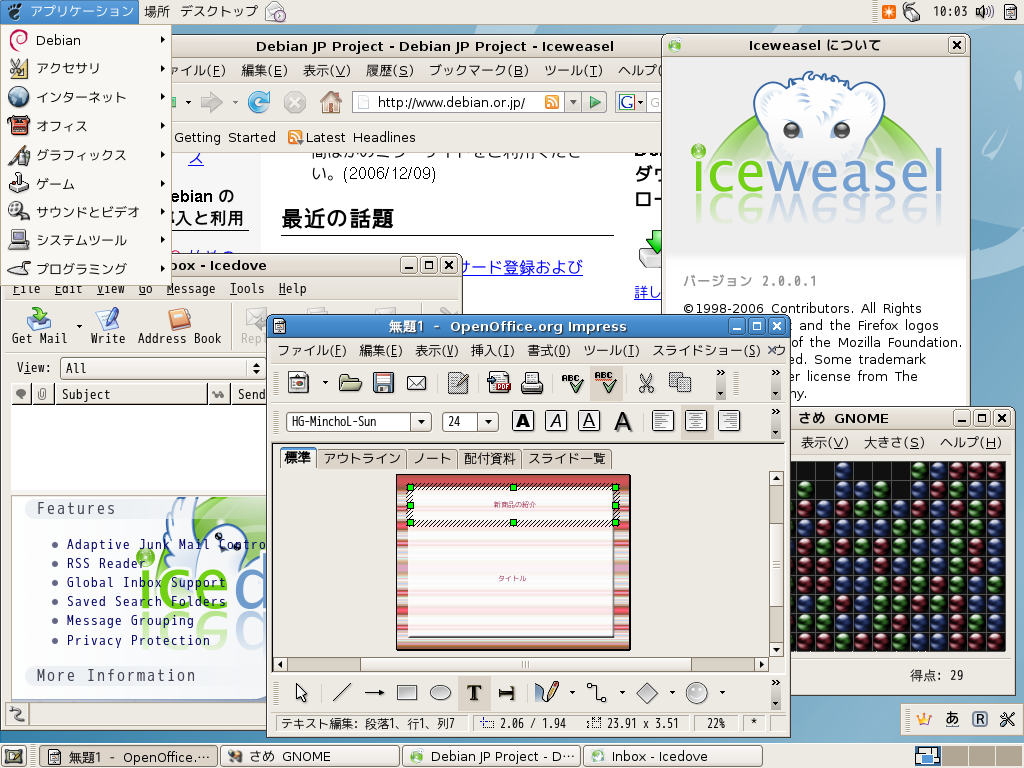
\includegraphics[width=5cm]{image201004/gnome.png}
        \caption{lenny $B$G$N(B Gnome $B$N2hLL(B}
    \end{center}
\end{wrapfigure}
\index{gnome}
GNOME $B$O(B GUI $B%D!<%k%-%C%H$K(B GTK+ $B$r;HMQ$7$?E}9g%G%9%/%H%C%W4D6-$G$9!#(B
Lenny $B$K<}O?$5$l$F$$$k$N$O(B 2.22$B!"(B
$B8=:_(B squeeze $B$K<}O?$5$l$F$$$k$N$O(B 2.30 $B$G$9!#(B(2010$BG/(B7$B7n8=:_(B)

Linux $B$K$*$$$F!VE}9g%G%9%/%H%C%W4D6-!W$H$$$&C18l$,L\N)$A;O$a$?;~$+$i(B KDE($B8e=R(B)$B$HAP`z$r$J$7$FH/E8$7$F$-$^$7$?!#(B
$B8=:_$G$O!VE}9g%G%9%/%H%C%W4D6-!W$H8@$($P!"$3$N(B GNOME $B$+(B KDE($B8e=R(B)$B$H8@$C$FNI$$$/$i$$N.9T$C$F$$$^$9!#(B
Debian $B$G$O%$%s%9%H!<%i$G(B GUI $B%$%s%9%H!<%k$rA*Br$9$k$H(B GNOME $B$N%G%9%/%H%C%W4D6-$,F3F~$5$l$^$9!#(B
$B$^$?!"(BUbuntu $B$G$bI8=`$G:NMQ$5$l$F$$$k$?$aFk@w$N$"$k?M$bB?$$$+$b$7$l$^$;$s!#(B

GNOME $B$r%$%s%9%H!<%k$9$k$K$O!"%?%9%/$+$i!V(BGnome $B%G%9%/%H%C%W4D6-!W$rA*$V$+!"F3F~$7$?$$%Q%C%1!<%8$NNL$K9g$o$;$F(B
\begin{description}
      \item[gnome] 
    GNOME $B4D6-A4$F(B(GNOME $B%W%m%8%'%/%H$,G[I[$7$F$$$J$$J*$b4^$a$k(B)
      \item[gnome-desktop-enviornment]
    GNOME $B%W%m%8%'%/%H$N8x<0G[I[J*$H$7$F$N(BGNOME $B4XO"$N%Q%C%1!<%8A4$F(B
      \item[gnome-accessibility]
    $BI,MW:G>.8B$N%Q%C%1!<%8$K%9%/%j!<%s%j!<%@$J$I$N>.J*$r2C$($?4D6-(B
      \item[gnome-core]
    $BI,MW:G>.8B$N4D6-!#%"%W%j%1!<%7%g%s$OJLESF3F~$9$kI,MW$,$"$k(B
\end{description}
$BEy$N%a%?%Q%C%1!<%8$r%$%s%9%H!<%k$7$^$9!#(B

$B$=$NB>!"(BDebian$B$G$N(BGNOME$B$K$D$$$F$O!"(BDebian GNOME Packaging $B$K>pJs$,=8$^$C$F$$$k$N$G;29M$K$9$k$H$h$$$G$7$g$&!#(B

\begin{itemize}
 \item Debian GNOME Packaging

       \url{http://pkg-gnome.alioth.debian.org/}

\end{itemize}


\subsubsection{KDE -- the K Desktop Environment}
\begin{wrapfigure}{r}{5.5cm}
 \begin{center}
  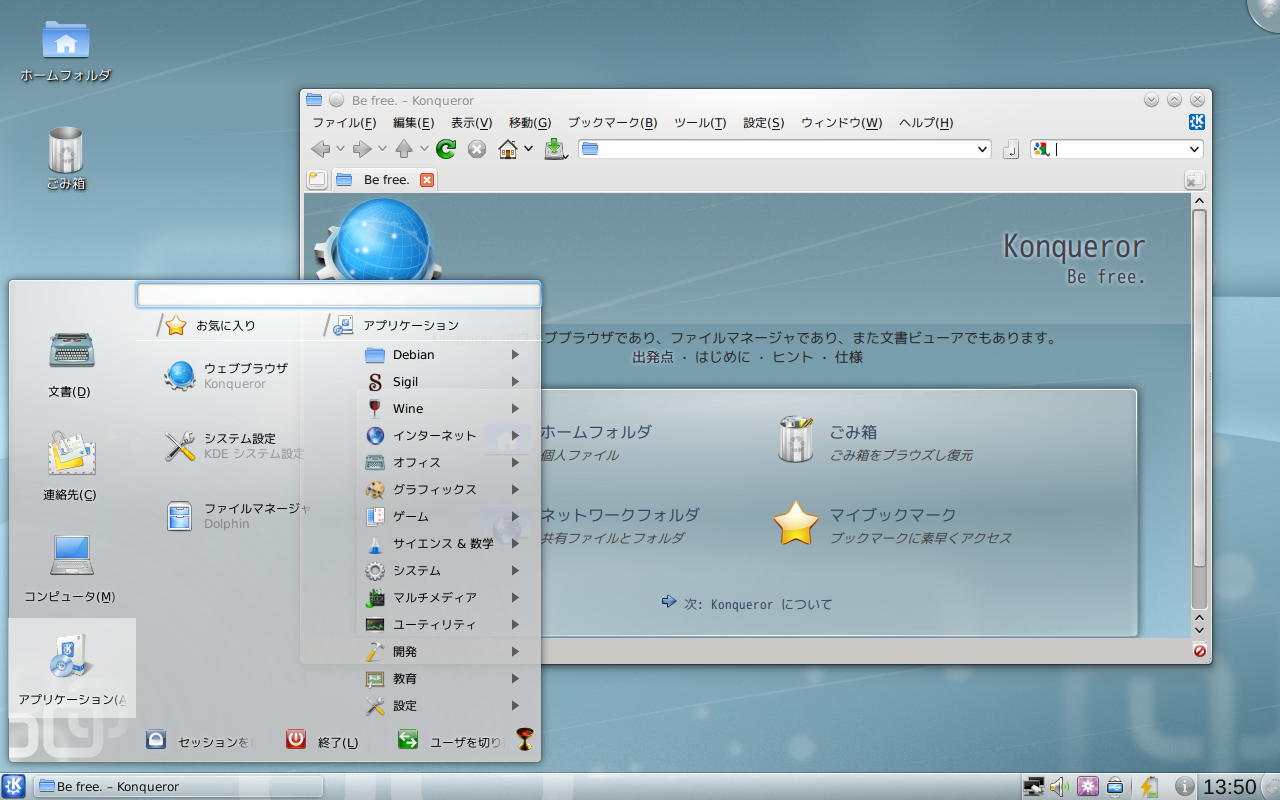
\includegraphics[width=5cm]{image201004/kde44.png}
  \caption{KDE 4.4$B$N2hLL(B}
 \end{center}
\end{wrapfigure}
\index{kde}

KDE$B$O!"(BGUI$B%D!<%k%-%C%H$K(BQt($B%-%e!<%H(B)$B$rMxMQ$7$?E}9g%G%9%/%H%C%W4D6-$G!"(B
Lenny$B$G$O%j%j!<%9$N%?%$%_%s%0$+$i(BKDE 3.5$B!"(Bsqueeze/sid$B$G$O(BKDE 4.4$B$,<}O?$5$l$F$$$^$9!#(B(2010$BG/(B7$B7n8=:_(B)

KDE 3$B7O$H(BKDE 4$B7O$O!"%D!<%k%-%C%H$,(BQt3$B$H(BQt4$B$,0c$&$[$+!"5!G=$d%G%9%/%H%C%W(B
$B<+BN$N9M$(J}$^$GJQ$o$C$F$$$k$N$G(BKDE 3$B7O$,9%$-$@$C$??M$O$H$^$I$&$+$b$7$l$^(B
$B$;$s!#(B

KDE$B$r%$%s%9%H!<%k$9$k$K$O!"%?%9%/$+$i!V(BKDE $B%G%9%/%H%C%W4D6-!W$rA*$V$+!"(B
$BF3F~$7$?$$%Q%C%1!<%8$NNL$K9g$o$;$F(B
\begin{description}
      \item[kde]
    KDE $B4D6-A4$F(B(KDE $B%W%m%8%'%/%H$,G[I[$7$F$$$J$$J*$b4^$a$k(B)
      \item[kde-core]
    $BI,MW:G>.8B$N4D6-!#%"%W%j%1!<%7%g%s$OJLESF3F~$9$kI,MW$,$"$k(B
\end{description}
$BEy$N%a%?%Q%C%1!<%8$r%$%s%9%H!<%k$7$^$9!#(B

$B$=$NB>!"(BDebian$B$G$N(BKDE$B$K$D$$$F$O!"(BDebian KDE Maintainers$B$N%5%$%H$K>pJs$,=8(B
$B$^$C$F$$$k$N$G;29M$K$9$k$H$h$$$G$7$g$&!#(B

\begin{itemize}
 \item The Debian KDE maintainers website:

       \url{http://pkg-kde.alioth.debian.org/}

\end{itemize}

\subsubsection{Xfce4}
\begin{wrapfigure}{r}{5.5cm}
 \begin{center}
  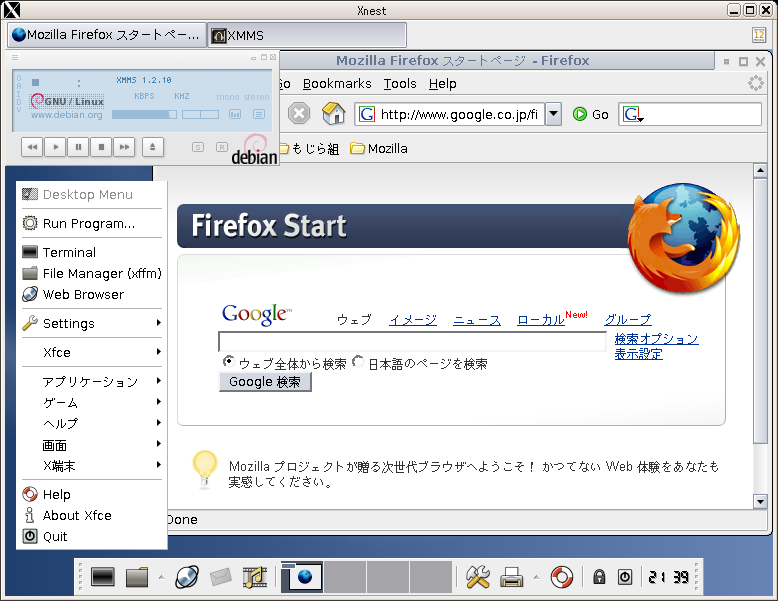
\includegraphics[width=5cm]{image201004/xfce4.png}
  \caption{Xfce4 $B$N2hLL(B}
 \end{center}
\end{wrapfigure}
\index{xfce4}

GNOME $B$d(B KDE $B$O$=$l$J$j$K%a%b%j$r6t$$$^$9$7!"$=$l$J$j$K=E$$$G$9!#(B
$B$=$3$G(B X $B$GMxMQ$G$-$k7ZNL$J%G%9%/%H%C%W4D6-$N9=C[$rL\I8$H$7$F:n@.$5$l$?$N$,(B
Xfce $B$G$9!#L>A0$NM3Mh$O(B {\it XForms Common Environment} $B$G$9!#(B
$B%P!<%8%g%s(B3 $B$^$G$O(B GUI $B%D!<%k%-%C%H$H$7$F(B XForms $B$r;HMQ$7!">&MQ(B UNIX $B$N(B CDE(Common Desktop Environment)$B$rLO$7$F$$$^$7$?$,!"(B
$B%P!<%8%g%s(B4 $B0J9_$O(BGUI $B%D!<%k%-%C%H$H$7$F(B GTK+2 $B$r;HMQ$7!"(B
$B$=$l$^$G$HJ70O5$$,$,$i$j$HJQ$o$j$^$7$?(B($B$=$s$JLu$G(B $B%P!<%8%g%s(B4 $B0J9_$r6/D4$9$k$?$a$K(B Xfce{\bf{4}} $B$H8F$V;v$bB?$$$G$9(B) $B!#(B

$BF1$8(B GTK+ $B$r;HMQ$7$F$$$k(B GNOME $B$HHf3S$7$F(B($B8+$?L\$be:No$J3d$K(B)$BHs>o$K7ZNL$KF0:n$9$k$N$,FCD'$G$9!#$^$?!"%W%m%8%'%/%H$N8x<0G[I[J*$G$O$J$$$b$N$N!"(BXfce Goodies $B$H8F$P$l$k%W%i%0%$%s$,B3!9$H3+H/$5$l$F$*$j!"Hs>o$K;H$$0W$$4D6-$H$J$C$F$$$^$9!#(B


Xfce4 $B$r%$%s%9%H!<%k$9$k$K$O!"%?%9%/$+$i!V(BXfce $B%G%9%/%H%C%W4D6-!W$rA*$V$+!"(B
{\tt xfce4} $B%Q%C%1!<%8$*$h$S(B {\tt xfce4-goodies}$B%Q%C%1!<%8$r%$%s%9%H!<%k$7$^$9!#(B


$B$=$NB>!"(BDebian$B$K$*$1$k(B Xfce $B$K4X$9$k>pJs$O(B Debian Xfce Group $B$N%5%$%H$K>pJs$,=8(B
$B$^$C$F$$$k$N$G;29M$K$9$k$H$h$$$G$7$g$&!#(B

\begin{itemize}
 \item Debian Xfce Group:

       \url{http://pkg-xfce.alioth.debian.org/}

\end{itemize}



\subsubsection{LXDE}
\begin{wrapfigure}{l}{5.5cm}
 \begin{center}
  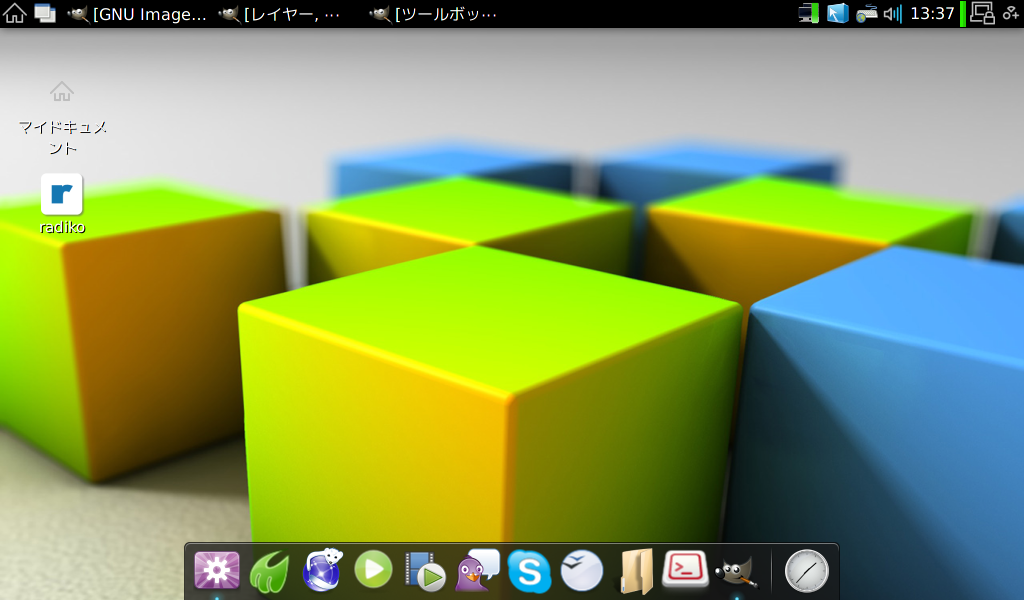
\includegraphics[width=5cm]{image201004/lxde-eeepc.png}
  \caption{LXDE$B$r(BeeePC$B$GMxMQ$7$F$$$k2hLL(B($B%i%s%A%c!<$O(BGNOME Do)}
 \end{center}
\end{wrapfigure}
\index{lxde}

LXDE$B$O=i4|5/F0;~$N%a%b%j;HMQNL$,(B100MB$B$[$I$N7ZNL$J%G%9%/%H%C%W4D6-$G$9!#(B

LXDE$B$O(BGNOME$B$d(BKDE$B!"(BXfce4$B$J$I$NB>$N%G%9%/%H%C%W4D6-$HHf3S$9$k$H!"E}9g%G%9%/(B
$B%H%C%W4D6-$H$7$F$N6&DL%i%$%V%i%j$J$I$,$J$/!"%&%#%s%I%&%^%M!<%8%c$K(B
OpenBox$B!"%U%!%$%k%^%M!<%8%c$K(BPCManFM$B!"%Q%M%k$K(Blxpanel$B$J$I7ZNL$N%"%W%j%1!<(B
$B%7%g%s$rAH$_9g$o$;!"$f$k$d$+$J7A$H$7$FE}9g%G%9%/%H%C%W4D6-$r<B8=$7$F$$$^(B
$B$9!#(B

Debian$B$G$N(BLXDE$B%Q%C%1!<%8$O(BAndrew Lee$B$5$s$,4IM}$7$F$$$^$9!#(B

$B%$%s%9%H!<%k$K$D$$$F$O(BKDE$B$HF1MM!"(Blxde$B$H$$$&%a%?%Q%C%1!<%8$,MQ0U$5$l$F$$$k(B
$B$N$G!"(Baptitude$B$GMF0W$K%$%s%9%H!<%k$G$-$^$9!#(B
\\
\begin{commandline}
$ sudo aptitude install lxde
\end{commandline}

LXDE$B$O:G?7HG$,(Bsqueeze$B$K<h$j9~$^$l$kM=Dj$G$9!#(B

% from debianmeetingresume201005-kansai.tex
\dancersection{$B<!4|%j%j!<%9$N(B squeeze $B$r8+$F$_$h$&(B}{$B$N$,$?$8$e$s(B}
\index{squeeze}

\subsection{$B$O$8$a$K(B}
Debian$B$J?M$J$iCN$C$F$k$3$H$b2~$a$F2r@b$7$J$,$i!"<!4|%j%j!<%9M=(B
$BDj$N(Bsqueeze$B$K$D$$$F2r@b$7$^$9!#(B

\subsection{squeeze$B$C$F2?(B?}
squeeze$B$H$O<!4|%j%j!<%9M=Dj$N(BDebian$B0BDjHG$N3+H/%3!<%I%M!<%`$G$9!#%P!<%8%g(B
$B%sHV9f$O(B6.0$B$G$9!#(BDebian$B$N3+H/%3!<%I%M!<%`$O!"1G2h(BToy Story$B$N%-%c%i%/%?!<(B
$BL>$+$i<h$i$l$F$F!"(Bsqueeze$B$O(B3$B$DL\$N%(%$%j%"%s$G$9!#(B

\subsection{$B$$$D%j%j!<%9$J$N(B?}
\label{sec:when-release-squeeze}

2009$BG/(B7$B7n$K3+:E$5$l$?(BDebConf 9$B$G%j%j!<%9$r%?%$%`%Y!<%9(B($B;~4V$G6h@Z$C$F(B)$B$N%j(B
$B%j!<%9$K0\9T$9$k$3$H$,H/I=$5$l$^$7$?!#(B\footnote{Debian decides to adopt
time-based release freezes:
\url{http://lists.debian.org/debian-announce/2009/msg00009.html}}$B$=$l$K$h(B
$B$k$H(B12$B7n%U%j!<%:(B($B?75,5!G=$J$I$NDI2CDd;_(B)$B!"MbG/(B3$B7n$K%j%j!<%9$NM=Dj$G$7$?!#(B

$B$7$+$7!"8=0BDjHG$N(BLenny$B$O(B2009$BG/(B2$B7n$K%j%j!<%9$5$l!"$^$@0lG/$b7P$C$F$$$J$$(B
$B>u67$G$OAa$9$.$k$H$NH=CG$+$i!"2~$a$F(B2010$BG/(B3$B7n$K%U%j!<%:$KF~$kM=Dj$G$7$?!#(B
\footnote{Bits from the release team: Planning, request for help:
\url{http://lists.debian.org/debian-devel-announce/2009/10/msg00002.html}}

$B$,!"$^$?0lE>!#(B3$B7n$K%M%C%H%o!<%/>c32$,5/$3$C$?$?$a!"$^$?;E@Z$jD>$7$K$J$j%U(B
$B%j!<%:$O(B5$B7nKv$+$i(B6$B7n>e=\$K1d4|$5$l(B\footnote{Bits from the Release Team:
Scheduling, transitions, how to help:
\url{http://lists.debian.org/debian-devel-announce/2010/04/msg00001.html}}
$B%j%j!<%9$OL$Dj$K$J$C$F$$$^$9!#(B

\subsection{squeeze$B$N%j%j!<%9%4!<%k(B}
squeeze$B$N%j%j!<%9L\I8$G$9$,!"8=:_$N$H$3$m(B2009$BG/$KH/I=$5$l$?%j%j!<%9%4!<%k(B
$B$+$iJQ$o$C$F$$$^$;$s!#0J2<!"(BDebian$B%K%e!<%9$N!V(BDebian GNU/Linux 6.0
"squeeze" $B%j%j!<%9$NL\I8!W$+$i$N0zMQ$G$9!#(B\footnote{Debian -- $B%K%e!<%9(B
-- Debian GNU/Linux 6.0 "squeeze" $B%j%j!<%9$NL\I8(B:
http://www.debian.org/News/2009/20090730}

\begin{itemize}
 \item $BB??t$N%"!<%-%F%/%A%c%5%]!<%H$K$h$k!"(B64 $B%S%C%H%^%7%s$X$N(B 32 $B%S%C%H(B
       $B%Q%C%1!<%8$N%$%s%9%H!<%k;v>p$N2~A1(B
 \item kFreeBSD $B%5%]!<%H!"(BDebian $B=i$N(B non-linux $B%"!<%-%F%/%A%c$NF3F~(B
 \item dash $B$r?7$7$$%G%U%)%k%H%7%'%k$H$7$F%V!<%H@-G=$r2~A1$7!"(B $B0MB8%Y!<%9(B
       $B$N%V!<%H%7%9%F%`$K$h$k%V!<%H%W%m%;%9$N%/%j!<%s%"%C%W$H(B $BJB9T=hM}$K(B
       $B$h$k@-G=8~>e$r?^$k(B
 \item $BIJ<AJ]>Z(B (QA) $B%W%m%;%9$r$5$i$K3HD%$7$F%Q%C%1!<%8$NIJ<A8~>e$K$D$J$2(B
       $B$k!#$=$NFbMF(B:
        \begin{itemize}
         \item $BA4%Q%C%1!<%8$K$D$$$F%/%j!<%s%$%s%9%H!<%k!"%"%C%W%0%l!<%I5Z(B
               $B$S:o=|(B
         \item $B4pACE*$JIJ<A%A%'%C%/$KDL$i$J$+$C$?%Q%C%1!<%8$N<+F05qH](B
         \item $B%@%V%k%3%s%Q%$%k$N%5%]!<%H(B
        \end{itemize}
 \item $B?7$7$$%Q%C%1!<%87A<0$r:vDj$7$F!"(B $B>-Mh$N3+H/$NG=N(2=$H05=L%"%k%4%j(B
       $B%:%`$N2~A1$r?^$k(B
 \item $B5l<0$N%i%$%V%i%j$r:o=|$7$F%;%-%e%j%F%#$r2~A1(B
 \item ipv6 $B$N40A4%5%]!<%H(B
 \item $B%i!<%8%U%!%$%k$N%5%]!<%H(B
 \item $B%"!<%+%$%VA4BN$N(B debug $B%Q%C%1!<%8$N<+F0@8@.!#(BGoogle Summer of
       Code $B%W%m%8%'%/%H$N%$%s%U%i$X$NE}9g$rJ]N1$7$F$$$^$9!#(B
 \item $B%Q%C%1!<%8$ND9$$@bL@$r(B\"$BK]Lu:Q$_%Q%C%1!<%8%j%9%H(B\"$B$KJ,N%$7$FK]Lu$r(B
       $BB%?J$7!"(B $B$^$?!"AH$_9~$_%7%9%F%`8~$1$K>.$5$/$7$?%U%C%H%W%j%s%H$rDs(B
       $B6!$7$^$9!#(B $B>.$5$/$J$C$?(B Packages $B%U%!%$%k$K46<U$7$^$9!#(B
 \item $B%Q%C%1!<%8$KJ#?t$NB0@-$r%?%0IU$1$9$k%7%9%F%`!"(Bdebtags $B$NE}9g$N2~A1(B
       $B$K$h$C$F%Q%C%1!<%8A*Br$r$b$C$H4JC1$K(B
 \item $B%a%s%F%J$K$h$j%"%C%W%m!<%I$5$l$?%P%$%J%j%Q%C%1!<%8$rGK4~!":F%S%k%I(B
       $B$7!"(B $B@)8f2<$N4D6-$G%S%k%I$5$l$?%Q%C%1!<%8$@$1$r;D$9(B
\end{itemize}

\subsection{$B:#!"$d$k$3$H$O(B?}

$B$^$@(B(2010$BG/(B5$B7n8=:_(B)$B%U%j!<%:$K$J$C$F$^$;$s!#JQ99E@$,$"$C$F$b$^$@4V$K9g$$$^$9!#(B($B$H$$$C$F$b(B
$BBgI}$JJQ99$O!V(B5$B7n(B21$BF|$^$G$KO"Mm$r!W$H8@$C$F$$$?$N$GFq$7$$$+$b$7$l$^$;$s$,!"(B
$BAjCL$9$k$3$H$,=EMW$@$H;W$$$^$9!#(B)

$B$=$l$^$G$K(BRelease Critical Bug($B%j%j!<%9$K>c32$H$J$k%P%0(B)$B$rDY$9$3$H!"K]Lu(B
$B$r?J$a$k$J$I!"$$$m$$$m$"$j$^$9!#(B

\subsection{$BF|K\8l4XO"$GCm0U$7$J$1$l$P$$$1$J$$$3$H(B}

$B$^$:(BDefoma$B$r;H$o$J$/$J$C$?$3$H$K$h$k1F6A$,$"$2$i$l$^$9!#(B

Debian$B$K$O(BDefoma(Debian Font Manager)$B$H$$$&%U%)%s%H$rFH<+$G4IM}$9$k;EAH(B
$B$_$,$"$j$^$9$,!"8=:_%a%s%F%J%s%9$5$l$F$*$i$:30$5$l$k$3$H$,7hDj$7$^$7$?!#(B

$B%G%9%/%H%C%W4D6-$G$O(BFontconfig$B$K$h$k%U%)%s%H4IM}$,$"$k$N$G(BDefoma$B$,30$5(B
$B$l$F$b1F6A$O$"$j$^$;$s$,!"(BTeX$B4D6-!"FC$KF|K\8l(BTeX$B4D6-$K$D$$$F$O(BDefoma$B$K(B
$B5!G=$r0MB8$7$F$$$?$3$H$b$"$j1F6A$,=P$k$3$H$,3NG'$5$l$F$$$^$9!#(B

$BF|K\8l(BTeX$B4D6-$G$N1F6A$O!"(BGhostScript$B$GF|K\8l(BPostScript$B$,07$($J$$!"(B
dvipsk-ja$B$,%S%k%I$G$-$J$$(B/$B;H$($J$$$J$I$"$j$^$9!#(B

TeX$B0J30$G$OF|K\8l(Bman$B$G$O(Bman$B$N@07A$r$9$k(Broff(groff)$B$,F|K\8l$NJ8;z$KCfES(B
$BH>C<$JBP1~$N$?$a!"$-$A$s$H@07A$7$FI=<($5$l$J$$$J$I$NLdBj$,3NG'$5$l$F$$(B
$B$^$9!#(B

$B$3$l$i$NLdBj$K$D$$$F!"@hF|!"BP1~$9$k%F%9%H%Q%C%1!<%8$H(BDebian JP$B$N%"%J%&%s(B
$B%9$,=P$?$N$G!"$46(NO$$$?$@$1$kJ}$O%"%J%&%s%9$rFI$s$G!"(BDebian JP Devel ML
$B$GH?1~$7$F$/$@$5$$!#(B\footnote{[debian-announce:00067] $B!V(Bsqueeze$B!W%j%j!<%9(B
$B$K8~$1$F2r7h$,I,MW$J%Q%C%1!<%8$N3+H/!&8!>Z6(NO$N$*4j$$(B:
\url{http://lists.debian.or.jp/debian-announce/201005/msg00003.html}}

$B$^$?!"LdBj$G$O$"$j$^$;$s$,!"IpF#$5$s$h$j(Buim$B$+$i(BIBus$B$X$NJQ99$NDs0F$,(B
Debian JP Devel ML$B=P$5$l$F$$$F!"0U8+$r5a$a$F$$$k$N$G!"4X?4$N$"$kJ}$O$40U(B
$B8+$J$I$r$*4s$;$/$@$5$$!#(B\footnote{[debian-devel:17817] Re: $BF|K\8l%?%9%/(B
(squeeze):
\url{http://lists.debian.or.jp/debian-devel/201005/msg00006.html}}


% =======================================================================
% from debianmeetingresume201002.tex
\dancersection{$B%V!<%HJ}K!$,JQ$o$k$h(B}{$B$^$($@$3$&$X$$(B}
\index{upstart}
\index{sysvinit}
% =======================================================================

\subsection{squeeze $B$+$i%V!<%HJ}K!$,JQ$o$k(B}
Debian $B$N%V!<%H$N;EAH$_$K$O!"(BSystem-V $B7O(B Unix $B$G$OEAE}E*$J(B init
(sysvinit) $B$,;H$o$l$F$$$^$9!#(BDebian $B$N<!4|0BDjHG(B6.0 ($B%3!<%I%M!<%`(B
Squeeze) $B$+$i!"$3$l$,(B upstart $B$KJQ$o$kM=Dj$G$9!#:#G/$N(B 3 $B7n$K%U%j!<%:M=(B
$BDj!"(B8$B7n$K%j%j!<%9M=Dj$N(BSqueeze $B$G$NM==,$N0UL#$r9~$a$F(B\footnote{$B:#2s$bM=(B
$BDjDL$jCY$l$F$$$^$9!#CY$l$?M}M3$O(B\ref{sec:when-release-squeeze}$B!V<!4|%j%j!<(B
$B%9$N(BSqueeze$B$r8+$F$_$h$&!W$N!V$$$D%j%j!<%9$J$N!)!W$r;2>H!#(B}$B!":#2s$O$3$N(B
upstart $B$KJQ$o$k$3$H$K$J$C$?GX7J!"(Binit $B$H$NHf3S$r4^$a$?(B upstart $B$N;EAH$_!"(B
$B<B:]$K@Z$jBX$(J}K!$K$D$$$F@bL@$7$^$9!#(B

\subsubsection{$BGX7J(B}

upstart $B$O!"(BDebian $B$r%Y!<%9$H$7$?%G%#%9%H%j%S%e!<%7%g%s$G$"$k(BUbuntu $B$G!"FH(B
$B<+$K(B sysvinit $B$N8e7Q$N;EAH$_$H$7$F3+H/$5$l$^$7$?!#85!9(B sysvinit $B$OEAE}E*(B
$B$G0BDj$7$?;EAH$_$G$O$"$j$^$9$,!"8=:_;H$o$l$F$$$k%O!<%I%&%'%"$G;H$&$K$O5!(B
$BG=LL!"@-G=LL$+$iLdBj$,=P$F$-$F$$$^$9!#$=$3$G!"(Bsysvinit $B$N8e7Q$N;EAH$_$H(B
$B$7$F!"(Bupstart $B0J30$K$bJ#?t$N%V!<%H%W%m%;%9$N;EAH$_$,3+H/$5$l$F$$$^$9!#$7(B
$B$+$7!"(BUbuntu $B0J30$K$b(B Fedora $B!"$^$?(B Google $B$N(B Chrome OS, Chromium OS $B$G(B
$B$b(B upstart $B$,:NMQ$5$l$F$$$^$9!#(BDebian $B$G$b(B squeeze $B$+$i:NMQ$5$l$kM=Dj$H(B
$B$$$&$3$H$b$"$j!"(Bsysvinit $B$N8e7Q$O(B upstart $B$KMn$ACe$/2DG=@-$,9b$$$N$G$O$J(B
$B$$$G$7$g$&$+!#(B

\subsubsection{$B$=$b$=$b(B init $B$C$F2?$h!)(B}

upstart $B$NOC$r$9$kA0$K!"(Binit $B$C$F2?!)$H$$$&?M8~$1$K$^$:@bL@$7$^$7$g$&!#(B
init $B$O:#99@bL@$7$J$/$F$bCN$C$H$k$,$J!"$H$$$&FI<T$O!"@h$KFI$_?J$a$F$/$@(B
$B$5$$!#(B

init $B$O(B Unix/Linux $B%7%9%F%`$K$*$$$F!"%+!<%M%k$,%V!<%H$7$?8e!"%f!<%6%W%m(B
$B%0%i%`$,5/F0$9$k$?$a$N;EAH$_$G$9!#Nc$($P!"$"$J$?$N;H$C$F$$$k%N!<%H(B PC $B$d(B
$B%5!<%P$KF~$C$F$$$k(B Debian $B%7%9%F%`$G$b$3$N;EAH$_$,I,$:F~$C$F$$$^$9!#%^%7(B
$B%s$KEE8;$rF~$l$F$+$i!"%m%0%$%s2hLL$,I=<($5$l$k$^$G$NN.$l$OBg$^$+$K$O(B
\fgref{fig:upstart-sysvinit-bootimage}($B%V!<%H$NN.$l(B)$B$N$h$&$K$J$j$^$9!#(B

\begin{figure}[H]
\begin{center}
\includegraphics[height=0.5\hsize]{image201002/sysvinit.eps}
\caption{$B%V!<%H$NN.$l(B}
\label{fig:upstart-sysvinit-bootimage}
\end{center}
\end{figure}

init $B%W%m%;%9$,5/F0$9$k$H!"(Binit $B$O(B /etc/inittab $B$NFbMF$K=>$C$F!"%W%m%;%9(B
$B$N$r@8@.$dDd;_$r9T$$$^$9!#(Binittab $B$N=q<0$O<!$N$h$&$K$J$j$^$9!#(B

\begin{commandline}
id:runlevels:action:process
\end{commandline}

Debian $B%7%9%F%`$N%G%U%)%k%H%i%s%l%Y%k$O(B 2 $B$J$N$G!"%W%m%;%9$N@8@.$K4X$o$k(B
$B4pK\E*$J%(%s%H%j$O<!$N(B4$B9T$G$9!#(B

\begin{commandline}
id:2:initdefault:                     $B"+%G%U%)%k%H%i%s%l%Y%k$O(B2
si::sysinit:/etc/init.d/rcS           $B"+5/F0;~$OI,$:<B9T(B
l2:2:wait:/etc/init.d/rc 2            $B"+%i%s%l%Y%k(B 2$B$G<B9T!#(B
1:2345:respawn:/sbin/getty 38400 tty1 $B"+(B getty $B$r>oCs(B
\end{commandline}

$B0l9TL\(B(id$B$,(Bsi)$B$K%i%s%l%Y%k$N;XDj$,L5$$$N$O!"(Baction $B$K(B sysinit $B$,;XDj$5$l$F$$$k$?(B
$B$a$G$9!#$3$l$O%9%F%`%V!<%HCf$K<B9T$5$l!"B>$N%V!<%HMQ$N(B action $B$h$j$bM%@h(B
$B$7$F<B9T$5$l$^$9!#(B/etc/init.d/rcS $B$NCf$G$O(B

\begin{commandline}
exec /etc/init.d/rc S
\end{commandline}

$B$@$1$,<B9T$5$l$^$9!#$3$N%o%s%i%$%J!<$O(B /etc/init.d/rc $B$G$N%V!<%HMQ$NJQ?t$r@_Dj$7$^$9!#(B
$B$3$N8e!">e5-$N(B rc $B%9%/%j%W%H$KBP$7!"5/F0;~$K;XDj$9$k%i%s%l%Y%k$r0z?t$H(B
$B$7$F<B9T$5$l$^$9$,!"(BDebian $B$G$N%G%U%)%k%H%i%s%l%Y%k$O(B2$B$G$9!#(B

\begin{commandline}
id:2:initdefault:
\end{commandline}

$B$G$9$N$G!"<B:]$K$O2<5-$,<B9T$5$l$^$9!#(B

\begin{commandline}
l2:2:wait:/etc/init.d/rc 2
\end{commandline}

$B$H$@$1$,<B9T$5$l$^$9!#$3$l$O%i%s%l%Y%k(B S $B$N%7%s%0%k%f!<%6%b!<%I$N$H$-$N$b(B
$B$N$G$9!#>e5-(B3$B9TL\$G%i%s%l%Y%k(B 2$B$N$H$-$K<B9T$5$l$k%(%s%H%j$,$"$k$3$H$+$i(B
$B$bJ,$+$k$H$*$j!"(B
\begin{enumerate}
 \item $B%i%s%l%Y%k(B S$B$N%W%m%;%9$,<B9T(B
 \item $B%i%s%l%Y%k(B 2$B$N%W%m%;%9$,<B9T(B
\end{enumerate}
$B$N=g$G5/F0%W%m%;%9$,<B9T$5$l$^$9!#%i%s%l%Y%k(B S $BMQ$N5/F0=hM}$,=*$o$C$F$+(B
$B$i!"%i%s%l%Y%k(B 2 $BMQ$N5/F0=hM}$,<B9T$5$l$k$N$G$9$+$i!"(B/etc/rcS.d/ $B0J2<$H(B
/etc/rc2.d/ $B0J2<$rHf3S$7$F$bJ,$+$k$H$*$j!"$3$l$,C`<!<B9T$5$l$k$N$O$+$J$j(B
$B;~4V$,$+$+$k$G$7$g$&!#$?$@$7!"F1$8%l%Y%k$N%9%/%j%W%H$OJB9T$7$F<B9T$5$l$k(B
$B$h$&$K2~A1$O$5$l$F$$$^$9!#(B

\begin{commandline}
# Now run the START scripts for this runlevel.
# Run all scripts with the same level in parallel
CURLEVEL=""
for s in /etc/rc$runlevel.d/S*
do
        # Extract order value from symlink
        level=${s#/etc/rc$runlevel.d/S}
        level=${level%%[a-zA-Z]*}
        if [ "$level" = "$CURLEVEL" ]
        then
                continue
        fi
        CURLEVEL=$level
        SCRIPTS=""
        for i in /etc/rc$runlevel.d/S$level*
        do
                [ ! -f $i ] && continue

                suffix=${i#/etc/rc$runlevel.d/S[0-9][0-9]}
(snip)
                SCRIPTS="$SCRIPTS $i"
                if is_splash_stop_scripts "$suffix" ; then
                        $debug splash_stop || true
                fi
        done
        startup $ACTION $SCRIPTS
done
\end{commandline}

$B5/F0%9%/%j%W%H$N5/F00J30$K$O!"%i%s%l%Y%k(B 2 $B$+$i(B 5 $B$^$?$O!"(B2 $B$+(B 3 $B$N;~$K(B
$B$O%3%s%=!<%k$+$i(B getty $B$,<B9T$5$l$^$9!#(Baction $B$,(B \texttt{respawn} $B$H$J$C(B
$B$F$$$^$9$,!"$3$l$O(B getty $B%W%m%0%i%`$,=*N;$7$?$i!"(Binit $B$,:F5/F0$5$;$k$?$a(B
$B$N;X<($G$9!#$"$k%f!<%6$,%3%s%=!<%k$+$i%m%0%$%s$7$?%;%C%7%g%s$r!"%m%0%"%&(B
$B%H$9$k$H(B getty $B$O=*N;$7$^$9$,!"(Binit $B$K$h$j:F$S(B $B%m%0%$%s2hLL$GBT$A<u$1$k(B
$B$3$H$,$G$-$k!"$H$$$&$o$1$G$9!#(B

\begin{commandline}
1:2345:respawn:/sbin/getty 38400 tty1
2:23:respawn:/sbin/getty 38400 tty2
3:23:respawn:/sbin/getty 38400 tty3
4:23:respawn:/sbin/getty 38400 tty4
5:23:respawn:/sbin/getty 38400 tty5
6:23:respawn:/sbin/getty 38400 tty6
\end{commandline}

init $B$NB>$NLr3d$H$7$F$O!"%7%9%F%`Dd;_;~$N%W%m%;%9$NDd;_$K$b4X$o$C$F$$$^(B
$B$9!#(B

\subsection{upstart $B$H$O(B}

$B$=$l$G$O!"(Binit $B$K$D$$$F$NM=HwCN<1$rF@$?$H$3$m$G!"K\Bj$N(B upstart $B$KF~$j$^(B
$B$7$g$&!#(Bupstart $B$O!!(Bsysvinit $B$r%$%Y%s%H%Y!<%9$KCV$-49$($?$b$N$G!"(B
$B%5!<%S%9$N3+;O$HDd;_$O%$%Y%s%H$NDL?.$K$b$H$E$-$^$9!#(Bupstart $B$N<g$JFCD'$O(B
$B<!$N(B 6 $B$D$G$9!#(B

\begin{itemize}
 \item $B%$%Y%s%H%I%j%V%s$G%?%9%/$d%5!<%S%9$r5/F0!&Dd;_$9$k!#(B
 \item $B%?%9%/$d%5!<%S%9$,5/F0!&Dd;_$9$k$3$H$G%$%Y%s%H$,H/@8$9$k!#(B
 \item $B%$%Y%s%H$O%7%9%F%`>e$NB>$N%W%m%;%9$+$i<u$1<h$k$3$H$,$G$-$k!#(B
 \item $B%5!<%S%9$,M=4|$;$:FMA3=*N;$7$F$b:F5/F0$9$k$3$H$,$G$-$k!#(B
 \item $B%G!<%b%s$N4F;k$H:F5/F0$O?F%W%m%;%9$+$iJ,N%$G$-$k!#(B
 \item D-Bus $B$rDL$8$F(B init $B%G!<%b%s$HDL?.$G$-$k!#(B
\end{itemize}

upstart$B$O!"(Bsysvinit$B$HF1MM$J5!G=$rDs6!$7$^$9$,!"(B\textbf{$BHsF14|%$%Y%s%H$K(B
$B1~$8$F<+N'E*$KF0:n$9$kE@(B}$B$,$b$C$H$b0[$J$j$^$9!#$=$N$?$a!"(Bsysvinit $B$KBP$9(B
$B$k(B upstart $B$N%a%j%C%H$K$O!"(B
\begin{itemize}
 \item $BMxMQ2DG=$J%O!<%I%&%'%"$@$1$G%V!<%H$9$k$?$a!"(Brunlevel $B$,I,MW$J$$!#(B
       $B$3$l$OB8:_$7$J$$%O!<%I%&%'%"$rI,MW$H$9$k%8%g%V$r%H%j%,!<$H$7$J$$(B
       $B$?$a!#(B
 \item $B%[%C%H%W%i%0%G%P%$%9$KBP1~(B
\end{itemize}
$B$H$$$C$?$3$H$,5s$2$i$l$^$9!#(B

$BNc$($P!"%7%9%F%`$,%V!<%H8e!"(BNIC$B$rA^$9$H(B
\begin{enumerate}
 \item network-interface-add $B%$%Y%s%H@8@.(B
 \item DHCP$B%8%g%V$,%M%C%H%o!<%/%+!<%I$r9=@.(B
 \item network-interface-up$B%$%Y%s%H$,@8@.(B
 \item $B%G%U%)%k%H%k!<%H$,?7$7$$%$%s%?%U%'!<%9$K3d$jEv$F(B
 \item default-route-up$B%$%Y%s%H$,@8@.(B
 \item NIC$B$rI,MW$H$9$k%8%g%V(B($B3F<o%5!<%P(B)$B$,<+F0E*$K3+;O$5$l$k(B
\end{enumerate}
$B$H$$$&F0$-$r$7$^$9!#5U$K%M%C%H%o!<%/%+!<%I$,$J$/$J$C$?>l9g$O<+F0E*$KDd;_$5$l$^$9!#(B

$B$?$@$7!"8=:_!"(Bsqueeze/sid$B$G:NMQ$5$l$F$$$k(B upstart $B$O!"(Bsysvinit $B$N8_49%b!<(B
$B%I$N$b$N$G$9!#(Bupstart $B$N:G=*L\I8$O!"%$%Y%s%H%I%j%V%s$N%V!<%H%W%m%;%9$K40(B
$BA4$K0\9T$9$k$3$H$G$9$,!"8_49%b!<%I$G$O!"(Bsysvinit $B$NF0:n$rLOJo$7$F$$$^$9!#(B
\footnote{$B$J$*!"(BUbuntu 9.10 $B0J9_$G$O(B $B%M%$%F%#%V%b!<%I$K0\9T$7$F$$$k$h$&(B
$B$G$9!#(B}

upstart $B$N>uBVA+0\$O(B\fgref{fig:upstart-stats}$B$N$h$&$K$J$j$^$9!#(B\footnote{upstart $B$N%I%-%e%a(B
$B%s%H$KIUB0$N$b$N$r7G:\!#(B}

\begin{figure}[h]
\begin{center}
\includegraphics[height=0.7\hsize]{image201002/states.eps}
\caption{upstart $B>uBVA+0\(B}
\label{fig:upstart-stats}
\end{center}
\end{figure}

\subsubsection{sysvinit $B$HJQ$o$i$J$$E@(B}
\label{se:same-sysvinit}

Debian $B$N(B upstart $B$O!"A0=R$N$H$*$j!"(BDebian $B%7%9%F%`$N5/F0!&Dd;_$H$$$&=EMW$JItJ,$N(B
$BCV$-49$($r9T$&$?$a8_49%b!<%I$N$b$N$,:NMQ$5$l$F$$$^$9!"2<5-$O(B sysvinit $B$H(B
$B;EMM>e$NJQ99$,$J$$ItJ,$G$9!#(B\footnote{$B$J$*!"(B\ref{se:same-sysvinit}$B!V(Bsysvinit$B$HJQ$o$i$J$$E@!W$H(B\ref{se:difference-sysvinit}$B!V(Bsysvinit$B$H0c$&E@!W$O(B upstart $B%Q%C%1!<%8$N(B README.Debian.gz $B$K5-:\$5$l$F$$$k(B FAQ $B$r$^$H$aD>$7$?$b$N$G$9!#(B}

\begin{itemize}
 \item initscript $B$,%$%s%9%H!<%k$5$l$k>l=j!#%Q%9$O(B /etc/init.d/$B!#(B
 \item $B5/F0!&Dd;_MQ$N(B initscript $B!#(B/etc/init.d/$B0J2<$+$i(B /etc/rc?.d/
       $B0J2<$K(B symlink $B$,D%$i$l$k!#(B
 \item $B5/F0!&Dd;_MQ(B initscript $B$N=g=x!#(BSNNname, KNNname $B$H$7$F(B symlink
       $B$rD%$k!#(BNN $B$O(B00$B$+$i(B99$B!#(BK$B%9%/%j%W%H$,:G=i$K=x?t=g$K<B9T$5$l!"(BS$B%9%/(B
       $B%j%W%H$,$=$N$"$H<B9T$5$l$k!#(B
 \item $B8=:_$*$h$S0l$DA0$N%i%s%l%Y%k$r3NG'$9$kJ}K!!#(B\texttt{runlevel} $B%3(B
       $B%^%s%I$r;H$&!#(B
 \item $B%i%s%l%Y%k$NJQ99J}K!!#(B\texttt{telinit} $B%3%^%s%I$+(B \texttt{init}
       $B%3%^%s%I$r<B9T$9$k!#(B
 \item $B%G%U%)%k%H$N%i%s%l%Y%k$NJQ99J}K!!#(B/etc/inittab $B%U%!%$%k$N(B
       \texttt{id:N:initdefault:}$B$N(BN$B$r=q$-49$($k!#(B
 \item $B%7%c%C%H%@%&%s$NJ}K!!#(Bupstart $B%Q%C%1!<%8$GDs6!$5$l$k!"(B
       \texttt{shutdown}$B%3%^%s%I$d(B \texttt{reboot}, \texttt{halt},
       \texttt{poweroff}$B$H$$$C$?%7%g!<%H%+%C%H$r;H$&!#%3%s%=!<%k$G(B
       Control-Alt-Delete $B$r2!$7$F%j%V!<%H=PMh$kE@$bF1$8!#(B
\item $B%7%s%0%k%f!<%6%b!<%I$K$9$kJ}K!!#(BGRUB $B$+$i(B\textbf{(recoveryode)}$B%*(B
      $B%W%7%g%s$rA*Br$+!"%+!<%M%k$N%3%^%s%I%i%$%s$G!"(B\texttt{-s, S,
      single}$B$J$I$N0z?t$r;XDj$9$k!#2TF/Cf$N%^%7%s$G$O!"(B\texttt{telinit
      1} $B$+(B \texttt{shutdown now}$B%3%^%s%I$r<B9T$9$k!#(B
\end{itemize}

\subsubsection{sysvinit $B$H0c$&E@(B}
\label{se:difference-sysvinit}

$B8_49%b!<%I$G$bA4$F$,(B sysvinit $B$HF0:n$,F1$8$H$$$&$o$1$G$O$J$/!"(Bupstart $B$N(B
$B8GM-$NItJ,$b$"$j$^$9!#<g$K(B getty $B4XO"$N@_Dj$,JQ$o$kE@$,Bg$-$J0c$$$G$9!#(B

\begin{itemize}
 \item Control-Alt-Delete $B$K$h$k5sF0$NJQ99J}K!!#(B
       /etc/init/control-alt-delete.conf$B$N(B\textbf{exec}$B$G;O$^$k9T$rJQ99(B
       $B$9$k!#%-!<$r2!$7$F$b2?$b<B9T$5$l$J$$$h$&$K$9$k$K$O!"%U%!%$%k$r:o(B
       $B=|$9$k$@$1!#(B
\begin{commandline}
(snip)
start on control-alt-delete

task
exec shutdown -r now "Control-Alt-Delete pressed"
\end{commandline}
 \item getty $B$r>oCs$5$;$k?t$r8:$i$9J}K!!#(B/etc/init/ttyN.conf $B%U%!%$(B
       $B%k$rJQ99$9$k(B\footnote{\textbf{N}$B$O(B1$B$+$i(B6$B$N?t;z(B}$B!#I,MW$J$1$l$P%U%!(B
       $B%$%k<+BN$r:o=|$9$k!#(B
 \item getty $B$N@_DjJQ99$NH?1GJ}K!!#%U%!%$%k$rJQ99$7$?$j:o=|$7$F$b$9$0$K$O(B
       $BH?1G$5$l$J$$!#(B\\
       $BDd;_$O(B\texttt{stop ttyN}$B%3%^%s%I$r!"5/F0$O(B\texttt{start ttyN}$B%3%^%s%I$r<B9T$9$k!#(B
 \item getty $B$N%Q%i%a!<%?$NJQ99J}K!!#(B/etc/init/ttyN.conf $B$N(B
       \textbf{respawn}$B$G;O$^$k9T$rJQ99$9$k!#(B
\begin{commandline}
# tty1 - getty
#
# This service maintains a getty on tty1 from the point the system is
# started until it is shut down again.

description     "Start getty on tty1"
author          "Scott James Remnant <scott@netsplit.com>"

start on stopped rc RUNLEVEL=[2345]
stop on runlevel [!2345]

respawn
exec /sbin/getty 38400 tty1
\end{commandline}
 \item getty $B$r<B9T$9$k%i%s%l%Y%k$NJQ99J}K!!#(B/etc/init/ttyN.conf $B$N<!(B
       $B$N(B2$B9T$rJQ99$9$k!#(B\\
       stop $B$N(B\textbf{!} $B$OH]Dj$G!"(Bstart $B$H(B stop$B$N@_Dj$O!"(B\textbf{!}$B0J30(B
       $B$O4pK\F1$8$K$9$k!#(B
 \item getty $B$N?t$rA}$d$9J}K!!#(B/etc/init/ttyN.conf$B$r!"(BttyS0$B$J$I$NL>A0$G%3(B
       $B%T!<$9$k!#(B\textbf{respawn}$B$N9T$KI,MW$J@_Dj$r$r5-=R$9$k!#(B
 \item $B%7%j%"%k%3%s%=!<%k$rDI2C$9$k>l9g$O!">e5-$N(B''getty $B$N?t$rA}$d$9J}K!(B''$B$HF1$8!#(B
 \item upstart $B$,F0$+$J$$>l9g$N%G%P%C%0J}K!!#%+!<%M%k%3%^%s%I%i%$%s$K(B
       \texttt{--debug}$B%*%W%7%g%s$r$D$1!"(B\texttt{quiet} $B$H(B
       \texttt{splash} $B%*%W%7%g%s$,$"$k>l9g$O$=$l$i$r:o=|$9$k!#(Bupstart
       $B$,<B9T$5$l$k$H%G%P%C%0%a%C%;!<%8$,=PNO$5$l$k!#(B
       \footnote{initramfs-tools $B$G$O$J$/(B initramfs $B@8@.%D!<%k$r;H$C$F$$(B
       $B$k>l9g$K$O$3$N%*%W%7%g%s$r;H$&$H4{CN$N%P%0$b$"$k$N$G5$$r$D$1$^$7$g$&!#(B}$B!#(B
 \item upstart $B$,F0$+$J$$>l9g$N%7%9%F%`I|5l<j=g!#(B
 \begin{enumerate}
  \item $B%+!<%M%k%3%^%s%I%i%$%s$+$i!"(B\texttt{quite}$B$H(B\texttt{splash}$B$,$"$l$P:o=|$7!"(B
	\texttt{init=/bin/bash}$B$r0z?t$H$7$F5/F0$9$k$H!"(Broot shell$B$,5/F0(B
	$B$5$l$k!#(B
  \item /etc/init.d/rcS $B$r<B9T$7$F!"%O!<%I%&%'%"$d%M%C%H%o!<%/$N4pK\@_Dj(B
	$B$r9T$&!#(B
  \item upstart $B$,$A$c$s$H%$%s%9%H!<%k$5$l$F$$$k$+3NG'$9$k!#(B/etc/init$B%G%#(B
	$B%l%/%H%j$KA4$F$N%U%!%$%k$,%$%s%9%H!<%k$5$l$F$$$k$+%A%'%C%/$7!"@5(B
	$B>o$K%$%s%9%H!<%k$5$l$F$J$$>l9g$O(B upstart $B%Q%C%1!<%8$r:F%$%s%9%H!<(B
	$B%k$9$k!#(B
  \item /etc/init $B$K%U%!%$%k$,:#EY$O$A$c$s$H$"$k$+3NG'$9$k!#(B
  \item \texttt{sync}$B$H(B\texttt{reboot -f}$B%3%^%s%I$r<B9T$7!"%^%7%s$r:F5/F0(B
	$B$9$k!#(B
 \end{enumerate}
 \item upstart $B%8%g%V%j%9%H$r%/%(%j$9$kJ}K!!#(B\texttt{initctl list}$B%3%^(B
       $B%s%I$G%8%g%V$H%9%F!<%?%9$rI=<($9$k!#(B
\begin{commandline}
$ sudo initctl list
tty4 start/running, process 25474
rc stop/waiting
tty5 start/running, process 25478
control-alt-delete stop/waiting
rcS stop/waiting
rc-sysinit stop/waiting
dbus-reconnect stop/waiting
tty2 start/running, process 25473
tty3 start/running, process 25475
tty1 start/running, process 25477
tty6 start/running, process 25476
\end{commandline}
 \item $B%8%g%V$N5/F0!&Dd;_J}K!!#(B\texttt{start JOB}, \texttt{stop JOB}
       $B%3%^%s%I$r<B9T$9$k!#(B
 \item $B%8%g%V$N%9%F!<%?%9I=<(J}K!!#(B\texttt{status JOB}$B%3%^%s%I!#(B
\begin{commandline}
$ sudo status tty1
tty1 start/running, process 25477
\end{commandline}
 \item $B<jF0$G%$%Y%s%H$rH/9T$9$kJ}K!!#(B\texttt{initctl emit EVENT}$B%3%^%s%I(B
       $B$GL>A0IU$-%$%Y%s%H$rH/9T$7!"BT5!Cf$N%8%g%V$,>u67$K1~$8$F5/F0(B or
       $BDd;_$9$k!#(B
\end{itemize}

\subsection{upstart $B$X$N@Z$jBX$((B}

$B$=$l$G$O!"AaB.(B sysvinit $B$+$i(B upstart $B$X@Z$jBX$($F$_$^$7$g$&!#(B
squeeze/sid $B$H(B Lenny $B$H$N>l9g$r8+$F$_$^$9!#(B

\subsubsection{squeeze/sid $B$G$N>l9g(B}

squeeze/sid $B$G$N(B upstart $B$X$N@Z$jBX$($K$O!"(Bupstart $B%Q%C%1!<%8$r%$%s%9%H!<(B
$B%k$7$^$9!#DL>o$N%Q%C%1!<%8$N%$%s%9%H!<%k$H$O0[$J$j!"B39T$9$k>l9g$O!"(B
\textbf{Yes, do as I say}$B$HF~NO$7$J$5$$!"$H$$$&%a%C%;!<%8$,I=<($5$l$^$9!#(B
$B$3$l$OF~$lBX$($OHs>o$K%j%9%/$,9b$$$?$a$G$9!#(B

\begin{commandline}
$ sudo apt-get install upstart
$B%Q%C%1!<%8%j%9%H$rFI$_9~$s$G$$$^$9(B... $B40N;(B
$B0MB84X78%D%j!<$r:n@.$7$F$$$^$9(B                
$B>uBV>pJs$rFI$_<h$C$F$$$^$9(B... $B40N;(B
$B0J2<$NFCJL%Q%C%1!<%8$,%$%s%9%H!<%k$5$l$^$9(B:
  dbus libdbus-1-3 libexpat1
$BDs0F%Q%C%1!<%8(B:
  dbus-x11
$B0J2<$N%Q%C%1!<%8$O!V:o=|!W$5$l$^$9(B:
  sysvinit
$B0J2<$N%Q%C%1!<%8$,?7$?$K%$%s%9%H!<%k$5$l$^$9(B:
  dbus libdbus-1-3 libexpat1 upstart
$B7Y9p(B: $B0J2<$NIT2D7g%Q%C%1!<%8$,:o=|$5$l$^$9!#(B
$B2?$r$7$h$&$H$7$F$$$k$+K\Ev$K$o$+$C$F$$$J$$>l9g$O!"<B9T$7$F$O$$$1$^$;$s(B!
  sysvinit
$B%"%C%W%0%l!<%I(B: 0 $B8D!"?75,%$%s%9%H!<%k(B: 4 $B8D!":o=|(B: 1 $B8D!"J]N1(B: 9 $B8D!#(B
1,005kB $B$N%"!<%+%$%V$r<hF@$9$kI,MW$,$"$j$^$9!#(B
$B$3$NA`:n8e$KDI2C$G(B 2,105kB $B$N%G%#%9%/MFNL$,>CHq$5$l$^$9!#(B
$B=EBg$JLdBj$r0z$-5/$3$92DG=@-$N$"$k$3$H$r$7$h$&$H$7$F$$$^$9!#(B
$BB39T$9$k$K$O!"(B'Yes, do as I say!' $B$H$$$&%U%l!<%:$r%?%$%W$7$F$/$@$5$$!#(B
 ?] Yes, do as I say!
\end{commandline}

lxc $B$N4D6-$G;n$7$F$_$^$7$?$,!"(Bgetty $B$,$&$^$/F0$+$:!"5/F0$7$F$OFMA3(B
$B;`$7$F!":F5/F0$5$l$F!"$^$?FMA3;`!"$H$$$&$N$r7+$jJV$7$F$7$^$&$N$G!"%3%s%=!<(B
$B%k$+$i$N%m%0%$%s$O=PMh$J$$>uBV$G$7$?$,(B\footnote{2010$BG/(B2$B7n(B9$BF|8=:_(B}$B!"(B
\ref{ch:re-startup-upstart}$B!V(Bupstart$B:FF~Lg!W$G(BKVM$B$N4D6-2<$G;n$7$?:]$K$O@5>o(B
$B$K5/F0$9$k$3$H$r3NG':Q$_$G$9!#(B

\begin{commandline}
$ sudo lxc-start -n bootsid
cat: /proc/cmdline: No such file or directory
Setting the system clock.
Cannot access the Hardware Clock via any known method.
Use the --debug option to see the details of our search for an access method.
Unable to set System Clock to: Tue Feb 9 14:16:26 UTC 2010 ... (warning).
Activating swap...done.
mount: you must specify the filesystem type
Cannot check root file system because it is not mounted read-only. ... failed!
Setting the system clock.
Cannot access the Hardware Clock via any known method.
Use the --debug option to see the details of our search for an access method.
Unable to set System Clock to: Tue Feb 9 14:16:27 UTC 2010 ... (warning).
Cleaning up ifupdown....
Checking file systems...fsck from util-linux-ng 2.16.2
done.
Setting up networking....
Mounting local filesystems...done.
Activating swapfile swap...done.
Cleaning up temporary files....
Configuring network interfaces...done.
Setting kernel variables ...done.
Cleaning up temporary files....
Starting system message bus: dbus.
Starting OpenBSD Secure Shell server: sshd.
init: tty4 main process (239) terminated with status 1
init: tty4 main process ended, respawning
init: tty5 main process (241) terminated with status 1
init: tty5 main process ended, respawning
init: tty2 main process (242) terminated with status 1
init: tty2 main process ended, respawning
init: tty3 main process (244) terminated with status 1
init: tty3 main process ended, respawning
init: tty6 main process (245) terminated with status 1
init: tty6 main process ended, respawning
init: tty1 main process (306) terminated with status 1
init: tty1 main process ended, respawning
init: tty4 main process (307) terminated with status 1
init: tty4 main process ended, respawning
(snip)
\end{commandline}

$B$3$N;~$b!"(Bssh $B7PM3$N%?!<%_%J%k%m%0%$%s$OLdBj$J$/$G$-$^$7$?!#(B

\begin{commandline}
$ ssh bootsid
Enter passphrase for key '/home/user/.ssh/id_rsa': 
Linux bootsid 2.6.32 #1 SMP Mon Dec 7 05:27:50 UTC 2009 x86_64

The programs included with the Debian GNU/Linux system are free software;
the exact distribution terms for each program are described in the
individual files in /usr/share/doc/*/copyright.

Debian GNU/Linux comes with ABSOLUTELY NO WARRANTY, to the extent
permitted by applicable law.
Last login: Tue Feb  9 14:18:38 2010 from 192.168.189.114
user@bootsid:~$ 
\end{commandline}

\subsubsection{Lenny $B$G$N>l9g(B}

squeeze/sid $B$G$b$&$^$/9T$C$F$$$J$$>u67$G$9$N$G!"(Bsqueeze $B$,(B stable $B$H$7$F(B
$B%j%j!<%9$5$l$k$H$-$K!"8!F$$7$^$7$g$&(B\footnote{upstart $B$,M=Dj$I$*$j(B squeeze $B$K4^$^$l$F(B
$B$$$k$3$H$,A0Ds$G$9$,!#(B}$B!#$"$k$$$O!"(Bsid $B$K%"%C%W%0%l!<%I$9$k$3$H$r8!F$$7(B
$B$F$bNI$$$G$7$g$&!#(B

\subsubsection{$B$^$H$a(B}

$B8=;~E@$G$O!"<B:]$K@Z$jBX$o$C$?:]$K$O%*%Z%l!<%7%g%s>e$bB?>/JQ99$,$"$j$^$9!#(B
Ubuntu 9.10 $B$G:NMQ$5$l$F$$$k(B $B%M%$%F%#%V%b!<%I$G$O99$K%*%Z%l!<%7%g%s$bJQ(B
$B$o$k$h$&$G$9$N$G!":#2s$O$8$a$F(B upstart $B$rCN$C$?$H$$$&J}$O!"<!>O$b;29M$N(B
$B>e!"Aa$a$K;H$$J}$d;EAH$_$rM==,$7!"%P%0=P$7$K6(NO$5$l$k$H(BDebian$B$NIJ<A$b8~(B
$B>e$9$k$3$H$G$7$g$&!#(B


% from debianmeetingresume201004.tex
\dancersection{upstart $B:FF~Lg(B}{$B$^$($@$3$&$X$$(B}
\subsection{$B$O$8$a$K(B}
$B:#G/$N(B2$B7n$N(B Debian $BJY6/2q!J(BDebian $B29@t!K(B\footnote{$BK\=q$G$OA0>O$K$"$?$j(B
$B$^$9!#(B}$B$G0lEY07$C$?%F!<%^$G$9!#:#2s$O5/F0B.EY$N4QE@$+$iJQ2=$,$"$k$+$r(B
$B8+$F$_$^$7$g$&!#(B
\footnote{4$B7n;~E@$G$O!"=q$-2<$m$9$D$b$j$G$7$?$,!"8D?ME*$JET9g$GM>M5$,$J(B
$B$/!":#2s$N;vA0G[I[;qNA$O4pK\E*$K!"(B2010$BG/(B2$B7n$N(B Debian $BJY6/2q$N;qNA!V%V!<(B
$B%HJ}K!$,JQ$o$k$h!W$r:FJT$7$?$@$1$@$C$?$N$G!"5/F0B.EY$N8!>Z$K$D$$$FEvF|H/(B
$BI=$N$_9T$$$^$7$?!#(B}

\subsubsection{$B;vA0=`Hw(B}
$BA0>O$H$O0[$J$j!"8!>Z$N$?$a$N4D6-$O(BKVM$B$GMQ0U$7!"5/F0B.EY$NHf3S$K$O(B
bootchart$B$rMQ$$$^$7$?!#(B
$BMQ0U$9$k%$%s%9%H!<%k%$%a!<%8$H!"%Q%C%1!<%8$O2<5-$NDL$j$G$9!#(B

 \begin{itemize}
  \item debian-testing-amd64-businesscard.iso
  \item qemu-kvm $B%Q%C%1!<%8(B
  \item qcow2 $B%U%)!<%^%C%H$N%G%#%9%/%$%a!<%8(B
  \item bootchart $B%Q%C%1!<%8(B
 \end{itemize}

KVM/QEMU$B%2%9%H$K$O!"(Bsysvinit$B$H(Bupstart$B$N(B2$B<oN`$rMQ0U$7$^$7$?!#(B
\begin{itemize}
 \item Debian GNU/Linux sid $B$N:G>.9=@.$r%$%s%9%H!<%k(B
 \item $B%$%s%9%H!<%k8e!"%G%#%9%/%$%a!<%8$+$i%3%T!<:n@.(B
 \item $B%3%T!<8e!"(Bupstart $B%Q%C%1!<%8$r%$%s%9%H!<%k(B
\end{itemize}

\subsubsection{upstart$B$N%$%s%9%H!<%k(B}

$BA0>O$G$b?($l$?ItJ,$G$9$,!":F7G$7$^$9!#(B
$B@Z$jBX$($K$O(B upstart $B%Q%C%1!<%8$r%$%s%9%H!<%k$7$^$9!#DL>o$N%Q%C%1!<%8$N%$%s%9%H!<%k$H$O0[$J$j!"B39T$9$k>l9g$O!"(B\textbf{Yes, do as I say}$B$HF~NO$7$J$5$$!"$H$$$&%a%C%;!<%8$,I=<($5$l$^$9!#(B
$B$3$l$O$&$^$/$$$+$J$$>l9g$O(B Debian $B%7%9%F%`$,5/F0$G$-$J$/$J$k$J$I$N%j%9%/(B
$B$,$"$k$?$a$G$9!#(B

\begin{commandline}
$ sudo apt-get install upstart
$B%Q%C%1!<%8%j%9%H$rFI$_9~$s$G$$$^$9(B... $B40N;(B
$B0MB84X78%D%j!<$r:n@.$7$F$$$^$9(B                
$B>uBV>pJs$rFI$_<h$C$F$$$^$9(B... $B40N;(B
$B0J2<$NFCJL%Q%C%1!<%8$,%$%s%9%H!<%k$5$l$^$9(B:
  dbus libdbus-1-3 libexpat1
$BDs0F%Q%C%1!<%8(B:
  dbus-x11
$B0J2<$N%Q%C%1!<%8$O!V:o=|!W$5$l$^$9(B:
  sysvinit
$B0J2<$N%Q%C%1!<%8$,?7$?$K%$%s%9%H!<%k$5$l$^$9(B:
  dbus libdbus-1-3 libexpat1 upstart
$B7Y9p(B: $B0J2<$NIT2D7g%Q%C%1!<%8$,:o=|$5$l$^$9!#(B
$B2?$r$7$h$&$H$7$F$$$k$+K\Ev$K$o$+$C$F$$$J$$>l9g$O!"<B9T$7$F$O$$$1$^$;$s(B!
  sysvinit
$B%"%C%W%0%l!<%I(B: 0 $B8D!"?75,%$%s%9%H!<%k(B: 4 $B8D!":o=|(B: 1 $B8D!"J]N1(B: 9 $B8D!#(B
1,005kB $B$N%"!<%+%$%V$r<hF@$9$kI,MW$,$"$j$^$9!#(B
$B$3$NA`:n8e$KDI2C$G(B 2,105kB $B$N%G%#%9%/MFNL$,>CHq$5$l$^$9!#(B
$B=EBg$JLdBj$r0z$-5/$3$92DG=@-$N$"$k$3$H$r$7$h$&$H$7$F$$$^$9!#(B
$BB39T$9$k$K$O!"(B'Yes, do as I say!' $B$H$$$&%U%l!<%:$r%?%$%W$7$F$/$@$5$$!#(B
 ?] Yes, do as I say!
\end{commandline}

2$B7n$N(B Debian $BJY6/2q;~E@(B\footnote{$BK\=q$G$OA0>O(B}$B$G$O!"(Blxc $B$N4D6-$G;n$7$?:](B
\footnote{2010$BG/(B2$B7n(B9$BF|8=:_(B}$B$O!"(Bgetty $B$,$&$^$/F0$+$:!"5/F0$7$F$OFMA3;`$7(B
$B$F!":F5/F0$5$l$F!"$^$?FMA3;`!"$H$$$&$N$r7+$jJV$7$F$7$^$$!"%3%s%=!<%k$+$i(B
$B$N%m%0%$%s$O=PMh$J$$>uBV$G$7$?$,!":#2s$N;qNA:n@.;~E@(B\footnote{2010$BG/(B4$B7n(B
11$BF|$K!"(BSqueeze Official Snapshot amd64 BC Binary-1 20100322-03:30$B$N(B ISO $B%$%a!<%8$r;HMQ$7$?:G>.9=@.!#(B}$B$G$O!"(BKVM$B4D6-$GLdBj$J$/5/F0$7$^$9!#%P!<%8%g%s$,JQ$o$C$F$^$;$s$,!"4D6-$,0[$J$k(B
$B$N$G860x$O8e<T$K$"$j$=$&$G$O$"$j$^$9!#(B

\subsubsection{$B5/F0B.EY$rHf$Y$F$_$k(B}
$B%W%m%;%9$rJB9T=hM}$5$;$k$3$H$G=hM}B.EY$r8~>e$5$;$k$N$G!"%W%m%;%9$,B?$$$[(B
$B$I!"8z2L$O9b$$$O$:$G$O$J$$$+!"$H$+9M$($i$l$^$9!#(B

$BHf3S$N$?$a$KMQ0U$7$?4D6-$O0J2<$NDL$j$G$9!#(B

\begin{itemize}
\item $B%V!<%H$N<oN`(B
\begin{itemize}
\item sysvinit$B$H(Bupstart
\end{itemize}
\item $B9=@.(B
\begin{itemize}
\item $B:G>.9=@.(B base$B$K(Bbootchart$B$r%$%s%9%H!<%k(B
\item CouchDB $B:G>.9=@.$K(Bcouchdb $B$r%$%s%9%H!<%k(B
\item LAMP CouchDB $B$N9=@.$K(Bapache2,rails, mysql-server$B$r%$%s%9%H!<%k(B
\item GNOME $B:G>.9=@.$K(B xserver-xorg, gnome $B$r%$%s%9%H!<%k(B 
\end{itemize}
\end{itemize}

\newpage

\subsubsection{bootchart$B$N7k2L(B}
\begin{figure}[thbp]
\subfigure[sysvinit]{\makebox[.45\linewidth][c]{
  \includegraphics[height=0.5\hsize]{image201004/upstart/sysvinit-bootchart.eps}}}
\subfigure[upstart]{\makebox[.45\linewidth][c]{
  \includegraphics[height=0.5\hsize]{image201004/upstart/upstart-bootchart.eps}}}
\caption{$B:G>.9=@.(B}
\end{figure}

\begin{figure}[thbp]
\subfigure[sysvinit]{\makebox[.45\linewidth][c]{
\includegraphics[height=0.5\hsize]{image201004/upstart/sysvinit-couchdb-bootchart.eps}}}
\subfigure[upstart]{\makebox[.45\linewidth][c]{
\includegraphics[height=0.5\hsize]{image201004/upstart/upstart-couchdb-bootchart.eps}}}
\caption{CouchDB}
\end{figure}

\begin{figure}[thbp]
\subfigure[sysvinit]{\makebox[.45\linewidth][c]{
\includegraphics[height=0.5\hsize]{image201004/upstart/sysvinit-lamp-bootchart.eps}}}
\subfigure[upstart]{\makebox[.45\linewidth][c]{
\includegraphics[height=0.5\hsize]{image201004/upstart/upstart-lamp-bootchart.eps}}}
\caption{LAMP}
\end{figure}

\begin{figure}[thbp]
\subfigure[sysvinit]{\makebox[.45\linewidth][c]{
\includegraphics[height=0.5\hsize]{image201004/upstart/sysvinit-desktop-bootchart.eps}}}
\subfigure[upstart]{\makebox[.45\linewidth][c]{
\includegraphics[height=0.5\hsize]{image201004/upstart/upstart-desktop-bootchart.eps}}}
\caption{GNOME}
\end{figure}

\clearpage
\subsubsection{$B7k2L(B}
$B5/F0B.EYD4::7k2L$r(B\tbref{tb:bootchart-check}$B$K<($7$^$9!#(B

\begin{table}[H]
\begin{center}
\caption{$B5/F0B.EYD4::7k2L(B}
\label{tb:bootchart-check}
\begin{tabular}{|c|c|c|c|c|}\hline
init$B$N<oN`(B & $B:G>.9=@.(B&
 CouchDB & LAMP & GNOME \\
\hline\hline
sysvinit & 5 sec & 6 sec & 8 sec & 8 sec \\
\hline
upstart & 5 sec & 6 sec & 8 sec & 8 sec \\
\hline
\end{tabular}
\end{center}
\end{table}

$B5/F0;~4V$K$O$^$C$?$/0c$$$,$"$j$^$;$s$G$7$?!#$,!"K\=q$rFI$s$G$$$kFI<T$N3'(B
$B$5$s$O4{$K$*5$$E$-$N$O$:!#(BDebian$B$N(Bupstart$B$O8_49%b!<%I$J$N$G!"(Bsysvinit$B$N(B
$BF0:n$rLOJo$7$F$$$k$N$G$7$?!#$3$l$G$OHf3S$K$J$j$^$;$s$M!#(B

\subsection{Ubuntu 9.10$B$r;n$7$F$_$?!#(B}

$B$=$3$G!"(BDebian$B$H$O<c439=@.$,JQ$o$j$^$9$,!"%M%$%F%#%V%b!<%I$N(Bupstart$B$K$J$C$F$$$k(BUbuntu 9.10$B$G;n$7$F$_$k$3$H(B
$B$K$7$^$7$?(B(\fgref{fig:ubuntu-upstart-check})$B!#0c$$$H$7$F$O!"0J2<$N$h$&$K(B
$B$J$j$^$7$?!#(B

\begin{itemize}
 \item init $B$N=hM}=*N;;~$G(B bootchart $B$N%m%0<}=8$r;_$a$k$o$1$G$O(B
       $B$J$$$h$&$@$,!"<B<AE*$K$O(B25$BICDxEY$G5/F0$,40N;!#(B
 \item $B$G$b5/F0%W%m%;%9$,JB9T=hM}$5$l$F$$$k$3$H(B Debian $B$G$N7k2L$rHf$Y$F(B
       $B$bJ,$+$j$^$9!#(B
\end{itemize}

\begin{figure}[thbp]
\begin{center}
\includegraphics[height=0.6\hsize]{image201004/upstart/ubuntu-karmic-20100417-3.eps}
\caption{Ubuntu 9.10$B$N(Bupstart}
\label{fig:ubuntu-upstart-check}
\end{center}
\end{figure}

%\newpage

\subsection{$B$^$H$a(B}
$B%M%$%F%#%V%b!<%I$8$c$J$$$H(B upstart $B$OK\Mh$N%a%j%C%H$,3h$+$;$J$$46$8$H$$(B
$B$&$3$H$,J,$+$j$^$7$?!#$H$O$$$(!"$$$-$J$j%M%$%F%#%V%b!<%I$N(B upstart $B$K@Z(B
$B$jBX$($k$N$O%j%9%/$"$k$N$G!"0l;~E*$K8_49%b!<%I$r;H$&$N$O;_$`$rF@$J$$$N$+(B
$B$b$7$l$^$;$s!#$?$@!"(BSqueeze $B$G$:$C$H8_49%b!<%I$J$N$b$I$&$+$H;W$$$^$9!#(B
SqueezeAndAHalf$B%j%j!<%9;~(B($B%j%j!<%9$5$l$k$J$i!"$G$9$,(B)$B$K%M%$%F%#(B
$B%V%b!<%I$K@Z$jBX$($i$l$k$H$&$l$7$$$+$b$7$l$^$;$s!#(B

$B7kO@$H$7$F$O!"!V$_$s$J$G;n$7$F%P%0=P$7$7$^$7$g$&!W$H$$$&$H$3$m$G$9!#(B

\subsection{$B;29M;qNA(B}

\url{http://www.ibm.com/developerworks/jp/linux/library/l-boot-faster/index.html}
\clearpage

% from debianmeetingresume201001-kansai.tex
\dancersection{Xen$B$G:n$k<+Bp%5!<%P(B}{$B@n9>(B $B9@(B}
\index{xen}

\subsection{$B$O$8$a$K(B}
$B6aG/!"(BCPU$B$N@-G=$,%Q%o%U%k$K$J$k$K$D$l$F!"9b2A$J%O!<%I%&%'%"$rA0Ds$H$7$?(B
$B2>A[2=5;=Q$,%Q!<%=%J%k%Y!<%9$G$b;H$($k$h$&$K$J$C$F$-$^$7$?!#(B

$B$=$3$G!"5S8w$rMa$S$F$-$?2>A[2=5;=Q$NBeI=3J$G$"$k(BXen$B$r;H$C$F!"%$%s%?%M%C(B
$B%H4XO"$N%5!<%P72$r9=C[$7$^$7$?$N$G!"(BDebian$B%Y!<%9$G(BXen$B$N2>A[%5!<%P$r9=C[(B
$B$9$k;~$KCm0U$9$k$3$H$d!">e5-%5!<%P72$r9=C[$9$k:]$K;W$C$?$3$H$r%l%]!<%H(B
$B$7$^$9!#(B

$B$^$?!"0J2<$N;EMM$O%Q!<%=%J%k%Y!<%9$G$N1?MQ$rA0Ds$K9=C[$7$?$b$N$G$9!#;E(B
$BMM$r;n$=$&$H$9$k$H$-$O!"I,$:%G!<%?Ey$N%P%C%/%"%C%W$r$H$C$F<+8J@UG$$G9T$C(B
$B$F$/$@$5$$!#$h$j>\$7$/CN$j$?$$J}$O@lLg=q$r;2>H$7$F$/$@$5$$!#(B

\subsection{Xen$B$H$O(B}
Xen$B$O!"2>A[%^%7%s%=%U%H%&%'%"$N0l$D$G!"(BOS$B$h$j(B1$B$D$N2<$N3,AX$G%O%$%Q!<%P(B
$B%$%6$H$$$&%W%m%0%i%`$rF0$+$9$b$N$G$9!#$3$N%?%$%W$O%O%$%Q!<%P%$%67?$H8F(B
$B$P$l!"!V(BVMware Infrastrucure$B!W$J$I$,$"$j$^$9!#(B

$BB>J}!"2>A[%^%7%s%=%U%H%&%'%"$K$O%"%W%j%1!<%7%g%s%?%$%W$H8F$P$l$k$b$N$,(B
$B$"$j!"!V(BVMware Workstation$B!W!V(BVirtualBox$B!W!V(BQEMU$B!W$,M-L>$G$9!#(B

\subsection{Xen$B$NFCD'(B}
Xen$B$O2>A[2=$9$k$?$a$N%b%G%k$H$7$F!"=`2>A[2=$H40A42>A[2=$N(B2$B$D$rDs6!$7$F$$$^$9!#(B
\begin{itemize}
\item $B=`2>A[2=(B(ParaVirtualization)\\
Xen$B$G$N=`2>A[2=$O%O!<%I%&%'%"$r%(%_%e%l!<%H$9$kBe$o$j$K!"2>A[%^%7%sMQ$N%O!<%I%&%'%"$r;HMQ$7$^$9!#$3$N%O!<%I%&%'%"$OA`:n$r$9$k$?$a$K%O%$%Q!<%P%$%6%3!<%k$r8F$S=P$7$^$9!#%O%$%Q!<%P%$%6%3!<%k$O2>A[%^%7%s4D6-$KBP1~$7!"(BOS$B$O(BXen$B2>A[%O!<%I%&%'%"MQ$K=$@5$9$kI,MW$,$"$j$^$9!#(B

\item $B40A42>A[2=(B(FullVirtualization)\\
Xen$B$O40A42>A[2=5!G=$bDs6!$7$F$$$^$9!#$3$N5!G=$rMxMQ$9$k$H!"%G%U%)%k%H$N(BOS$B$r$=$N$^$^(BXen$B>e$GF0:n$5$;$k$3$H$,$G$-$^$9!#(B
\end{itemize}

\subsection{Xen$B$N7ABV(B}
Xen$B$O(BLinux$B$r%Y!<%9$K:n$i$l$F$$$^$9$N$G!"(BXen$BMQ$K%3%s%Q%$%k$5$l$?%+!<%M%k$rMxMQ$7$^$9!#$3$N%+!<%M%k$O5/F0;~$K%O%$%Q!<%P%$%6$r%m!<%I$7!"$=$N>e$K%+!<%M%k$r%m!<%I$7$^$9!#%$%a!<%8E*$K$O%O%$%Q!<%P%$%6>e$r4IM}(BOS$B$N(BDomainO$B$,F0$-!"$=$N(BOS$B$K4IM}$5$l$k7A$G%2%9%H(BOS$B$H8F$P$l$k(BDomainU$B$,F0$-$^$9!#(B

\begin{itemize}
\item Domain-O $B!J4IM}(BOS$B!K0J2<(BDomO \\
      Xen$B$r5/F0$7$?(BOS$B!#%O!<%I%&%'%"$r4IM}$7!"%O%$%Q!<%P%$%6>e$GF0:n$9$k%2%9%H(BOS$B$N4IM}$r9T$&!#(B
\item Domain-U $B!J(BDomU-$B=`2>A[2=!K0J2<(BDomU \\
      Domain-O$B$K$h$C$F5/F0!"4IM}$5$l$k%2%9%H(BOS$B!#FC$K!"=`2>A[2=$GF0:n$9$k!#(B
\item HVM Domain $B!J(BHVM-$B40A42>A[2=!K0J2<(BHVM \\
      Domain-O$B$K$h$C$F5/F0!"4IM}$5$l$k%2%9%H(BOS$B$G$"$k$,!"40A42>A[2=$G$"$k(BHVM(Hardware Virtual Machine)$B$GF0:n$9$k!#(B
\end{itemize}

%$B?^7A$NA^F~(B
\begin{figure*}[h!]
 \centering
 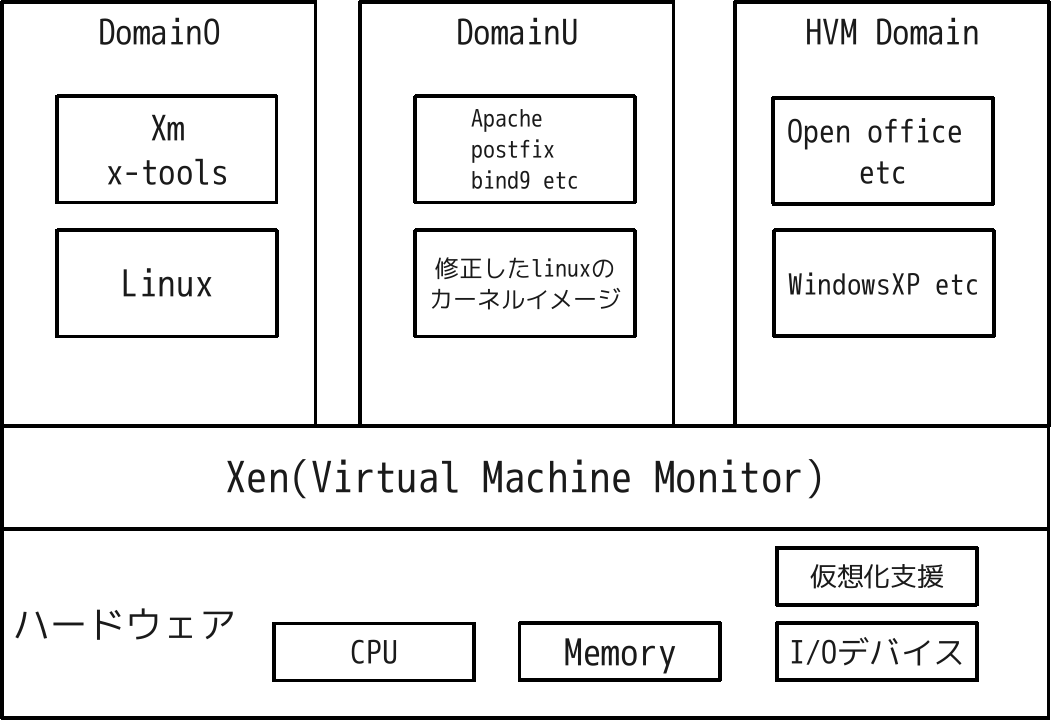
\includegraphics[scale=0.6]{image201001/xen-image.png}
 \caption{Xen $B$N%O%$%Q!<%P%$%6%b%G%k$N%$%a!<%8(B}
\end{figure*}
\clearpage

\subsection{Xen $B$NF3F~(B}
$B<!$K(B, Xen $B$r%$%s%9%H!<%k$7$^$9(B. $B%$%s%9%H!<%k$O3F%"!<%-%F%/%A%c$K$h$C$F0[$J$j$^$9(B. \footnote{$B>\$7$/$O(B, $B2>A[2=5;=Q(B Xen -$B35G0$HFbIt9=B$$J$I$r;2>H$7$F$/$@$5$$(B. $B40A42>A[2=$rL\E*$K$9$k$N$G$"$l$P(B Intel-VT $B$d(B AMV-V $B$,(B, CPU $B$G2>A[2=;Y1g5!G=$r;}$C$F$$$^$9(B. } $B$3$3$G$O(B, $B%$%s%F%k$r%Y!<%9$K(B Lenny $B$N(B Xen $B%+!<%M%k%$%a!<%8(B 2.6.26 $B$r0J2<$NMM$K%$%s%9%H!<%k$7$^$9(B.

\begin{commandline}
# aptitude install xen-linux-system-2.6.26-2-xen-686 
\end{commandline}
$B$^$?(B, Debian $B$K$O(B DomU $B$r:n$k%D!<%k$bMQ0U$7$F$"$j$^$9$N$G(B, $B$3$l$b%$%s%9%H!<%k$7$^$9(B.
\begin{commandline}
# aptitude install xen-tools
\end{commandline}
$B3F%$%s%9%H!<%k$,:Q$s$@$i(B, /xen/xen/xend-config.sxp $B%U%!%$%k$N0J2<$N2U=j$rJQ$($^$9(B.
\begin{commandline}
(network-script 'network-bridge netdev=eth1')
(network-script 'network-bridge netdev=eth0')
\end{commandline}
$B:F5/F0$7(B, DomO $B$N5/F0$r3NG'$7$^$9(B.
\begin{commandline}
# xm list
Name                 ID   Mem  VCPUs   State   Time (s)
Domain-0             0   1478     1   r-----    217.6
\end{commandline}

\subsection{DomU $B$N@_Dj(B}
Xen $B$N%D!<%k$r;H$C$F%2%9%H(B OS $B$r0J2<$N<j=g$GF~$l$^$9(B. (etch $B$d(B Ubuntu, CentOS $B$b2DG=(B).
\begin{enumerate}
\item $B@_Dj%U%!%$%k$NJT=8(B
\item xen-create-image $B$N<B9T(B
\item DomU $B$N5/F0(B
\end{enumerate}

\subsubsection{$B@_Dj%U%!%$%k$NJT=8(B}
$B@_Dj%U%!%$%k$O(B, /etc/xen-tools/xen-tools.conf $B$G$9(B. $B0J2<(B, DomU $B$K(B Lenny $B$r%$%s%9%H!<%k$b$N$H$7$FJT=8$7$^$9(B.

%$B2~%Z!<%8(B, $BCm0U(B
\begin{commandline}
##
#  /etc/xen-tools/xen-tools.conf
##             ($BCfN,(B)
#  Output directory for storing loopback images.
#
#  If you choose to use loopback images, which are simple to manage but
# slower than LVM partitions, then specify a directory here and uncomment
# the line.
#
#  New instances will be stored in subdirectories named after their
# hostnames.
# 
##
dir = /home/xen ($B%$%a!<%8%U%!%$%k$NJ]4I>l=j$G$9(B)
#              ($BCfN,(B)

##
#  Disk and Sizing options.
##
size   = 4Gb      # Disk image size.
#memory = 128Mb    # Memory size
memory = 384Mb    # Memory size
#swap   = 128Mb    # Swap size
swap   = 512Mb    # Swap size
# noswap = 1      # Don't use swap at all for the new system.
fs     = ext3     # use the EXT3 filesystem for the disk image.
#dist   = etch     # Default distribution to install.
dist   = lenny     # Default distribution to install.

#  Currently supported and tested distributions include:
#
# via Debootstrap:
#
#  Debian:
#   sid, sarge, etch, lenny.($BB>$N%G%#%9%H%j%S%e!<%7%g%s$NA*Br$b2DG=(B)
#
#  Ubuntu:
#   edgy, feisty, dapper.
#
# via Rinse:
#   centos-4, centos-5.
#   fedora-core-4, fedora-core-5, fedora-core-6, fedora-core-7

##
# Networking setup values.
##
#
## Uncomment and adjust these network settings if you wish to give your
# new instances static IP addresses.
#
# gateway   = 192.168.1.1
gateway   = 192.168.0.1
# netmask   = 255.255.255.0
netmask   = 255.255.255.0
# broadcast = 192.168.1.255
broadcast = 192.168.0.255
#($B%M%C%H%o!<%/$O$4<+M3$K(B)

#($B0J2<$O%G%U%)%k%H$K$7$^$7$?(B)
# Default kernel and ramdisk to use for the virtual servers
#
kernel      = /boot/vmlinuz-`uname -r`
initrd      = /boot/initrd.img-`uname -r`

#  The architecture to use when using debootstrap, rinse, or rpmstrap.
#
#  This is most useful on 64 bit host machines, for other systems it
# doesn't need to be used.
#
# arch=[i386|amd64]
#

# The default mirror for debootstrap to install Debian-derived distributions
#
mirror = http://ftp.jp.debian.org/debian/

#  If you're using the lenny or later version of the Xen guest kernel you will
# need to make sure that you use 'hvc0' for the guest serial device,
# and 'xvdX' instead of 'sdX' for serial devices.
#
#  You may specify the things to use here:
#
serial_device = hvc0 #default
# serial_device = tty1
#
disk_device = xvda #default
# disk_device = sda

#  Here we specify the output directory which the Xen configuration
# files will be written to, and the suffix to give them.
#
#  Historically xen-tools have created configuration files in /etc/xen,
# and given each file the name $hostname.cfg.  If you want to change
# that behaviour you may do so here.
#
# output    = /etc/xen
# extension = .cfg
#
\end{commandline}

\subsubsection{xen-create-image $B$N<B9T(B}
$B<!$K(B, DomU $B$N%$%a!<%8$r:n$j$^$9(B. $BF1;~$K(B DomU $B$K3d$jEv$F$k(B IP $B%"%I%l%9$r%*%W%7%g%s$G;XDj$7$^$9(B. $BNc$($P(B, $B%"%I%l%9$r(B 192.168.0.2, $B%[%9%H%M!<%`$r(B dns $B$H$9$k$J$i0J2<$N$h$&$K$7$^$9(B.
\begin{commandline}
# xen-create-image --ip 192.168.0.2 --hostname dns
\end{commandline}
DomU $B$N@):n$K$O(B, $B%$%a!<%8%G%#%9%/$NBg$-$5$d%M%C%H%o!<%/$N>u67$K$h$C$F0[$J$j$^$9$,(B, $B<+J,$N4D6-$G$O(B 10G $B$N%$%a!<%8$G(B 30 $BJ,$0$i$$$G$7$?(B.

\subsubsection{DomU $B$N5/F0(B}
$BL5;v$K(B, $B%$%s%9%H!<%k$,$G$-$?$i5/F0$7$F(B, $B2TF/>u67$r8+$F$_$^$7$g$&(B.
\footnote{Xen $B$K$O4IM}MQ%D!<%k$H$7$F!V(B xm $B!W$J$I$,$"$j$^$9(B. $B>\$7$/$O(B, Xen $BE0DlF~Lg$J$I$r;2>H$7$F$/$@$5$$(B. }
\begin{commandline}
# xen create -c dns.cfg
# xm list
 Name                                        ID   Mem VCPUs      State   Time (s)
 Domain-0                                     0  1478     4     r-----    429.8
 dns                                          5   384     1     -b----     10.5
 mail                                         2   384     1     -b----    123.6
 www                                          4  1792     1     -b----     23.1
\end{commandline}
$B5/F0$7$F$/$k2hLL$O(B, $BA4$/$N=i4|>uBV$G%m%0%$%s%W%m%s%W%H$7$+=P$^$;$s(B. root $B$G%m%0%$%s$7$F%Q%9%o!<%I$H%f!<%6$r:n@.$7$^$9(B.
\begin{commandline}
# passwd
# adduser ipv6waterstar
\end{commandline}
\subsubsection{$B%P%C%/%"%C%W(B, $BB>(B}
$B$^$?(B, DomU $B$r%G%U%)%k%H$G%$%s%9%H!<%k$7$?>l9g(B, DomO $B$N(B/home/xen/domain $B$K3F(B DomU $B$N%I%a%$%s$4$H$K%a!<%8%U%!%$%k$,CV$+$l$^$9(B. $B$^$?(B, $B@_Dj%U%!%$%k$O(B/etc/xen $B$K(B  ".cfg"$B%U%!%$%k$H$7$FJ]B8$5$l$^$9(B.

$B=>$C$F(B, $BNc$($P2?$i$+$N@_Dj%_%9$r$7$F(B DomU $B$,5/F0ITG=$K$J$C$F$b(B, $B>e5-$N%$%a!<%8$H@_Dj%U%!%$%k$N%P%C%/%"%C%W$,$"$l$P(B, $B3F%G%#%l%/%H%j$H@_Dj%U%!%$%k$r$=$N$^$^%3%T!<$7D>$9$@$1$G(B, $BF1$84D6-$N(B DomU $B$rI|85$G$-$^$9(B.

$B$^$?(B, $B4IM}MQ$N(B DomO $B$O%;%-%e%j%F%#$N4X78$+$i%W%m%;%9?t$,>/$J$$J}$,$$$$$N$G$9$,(B, $B8e=R$N$h$&$K@_Dj%U%!%$%k$rB??t(B, $B:n@.$9$k>l9g$N$3$H$b9M$($k$H(B, GUI $B$GA`:n$,$G$-$k$J$I$NMxE@$+$i(B, gnome $B$J$I$r%$%s%9%H!<%k$9$k$3$H$r4+$a$^$9(B.


\subsection{Xen $B$N%M%C%H%o!<%/$N35MW(B}
Xen $B$O2>A[%$%s%?!<%U%'%$%9$r%Y!<%9$K$7$?%M%C%H%o!<%/5!G=$r;}$C$F$$$^$9(B.

$B6qBNE*$K$O(B, DomU $B$N3F%[%9%H$rD>@\30It%M%C%H%o!<%/$K@\B3$9$k%V%j%C%87PM3$N@\B3(B. $B2>A[%$%s%?!<%U%'%$%9$rDL$7$F(B, DomO $B$N%k!<%F%#%s%0$7(B, $B%M%C%H%o!<%/%$%s%?!<%U%'%$%9$K=PNO$9$k%V%j%C%8$r7PM3$7$J$$@\B3(B (NAT $B@\B3(B) $B$NFs$D$N7ABV$,$"$j$^$9(B.

$B%V%j%C%87PM3$N@\B3$N%$%a!<%8$O%O!<%I%&%'%">e$K(B, DomO $B$HJ#?t$N(B DomU $B$N2>A[(B PC $B$,$"$C$F(B, $B$=$l$>$l$,BPEy$K%M%C%H%o!<%/%O%V$G7R$,$C$F$$$k$h$&$J>uBV$G$9(B.

$B:#2s$O(B, $B3F(B DomU $B%5!<%P$r%$%s%?!<%M%C%H%5!<%P$H$7$F1?MQ$7$?$$$N$G(B, $B2>A[%$%s%?!<%U%'%$%9$r;H$C$FD>@\(B, $B%;%0%a%s%H$,0[$J$k30It%M%C%H%o!<%/$K@\B3$G$-$k%V%j%C%87PM3$N@\B3$G%M%C%H%o!<%/$r9=@.$7$^$9(B.

DomU $B$O2>A[%^%7%s$r:n@.$9$k$H$-$K(B, IP $B%"%I%l%9$r3d$jEv$F$?$N$GFCJL$J@_Dj$OI,MW$"$j$^$;$s(B. $BF1;~$K(B, Mac $B%"%I%l%9$b3F2>A[%$%s%?!<%U%'%$%9$4$H$K<+F0E*$K3d$jEv$F$i$l$^$9(B.

$B$^$?(B, IP $B%"%I%l%9$r8e$+$iJQ99$7$?$$$H$-$J$I$O(B/etx/xen $B0J2<$N(B".cfg"$B%U%!%$%k$r=q$-49$($^$9(B.

$BNc(B  dns.cfg
%$B2~%Z!<%8(B  $BCm0U(B
\begin{commandline}
#
# Configuration file for the Xen instance www, created
# by xen-tools 3.9 on Tue Nov 17 10:35:03 2009.
#

#
#  Kernel + memory size
#
kernel      = '/boot/vmlinuz-2.6.26-2-xen-686'
ramdisk     = '/boot/initrd.img-2.6.26-2-xen-686'
memory      = '384'($B%a%b%j!<$NMFNL$NJQ99$b2DG=(B)

#
#  Disk device (s).
#
root        = '/dev/xvda2 ro'
disk        = [
                  'file:/home/xen/domains/www/swap.img,xvda1,w',
                  'file:/home/xen/domains/www/disk.img,xvda2,w',
              ]


#
#  Hostname
#
name        = 'dns'($B%[%9%HL>(B)

#
#  Networking
#
vif         = [ 'ip=192.168.0.2,mac=00:12:34:56:78:9A' ]
($B%"%I%l%9$NJQ99$b2DG=$G$9$,(B, DomU $B$N(B interfaces $B$r=q$-49$($F$$$k$H$-$O$=$A$i$b=q$-49$($F$/$@$5$$(B)

#
#  Behaviour
#
on_poweroff = 'destroy'
on_reboot   = 'restart'
on_crash    = 'restart'
\end{commandline}

\subsubsection{$B3F%$%s%?!<%M%C%H%5!<%P$N@_Dj$9$kA0$NCm0U;v9`(B}
$B<!$K(B, DNS, Mail $B%5!<%P(B, Web $B%5!<%P$N%Q%C%1!<%8$r(B, $B3F(B DomU $B$K%$%s%9%H!<%k$7$^$9(B.

$B%$%s%9%H!<%k$O(B, $B2>A[%^%7%s$G$b%N!<%^%k$N%$%s%9%H!<%k$HJQ$o$j$^$;$s(B. $B$?$@(B, Xen $B$N%M%C%H%o!<%/9=@.$OFHFC$N!VJJ!W$N$h$&$J$b$N$,$"$j$^$9(B. $B0J2<(B, $B$$$/$D$+Nc$r5s$2$^$9(B.
\begin{enumerate}
\item NTP $B$r;H$C$?;~4V$N@_Dj(B 
\item SSH $B$G$N%m%0%$%s(B
\item $B$=$NB>(B 
\end{enumerate}

\subsubsection{NTP $B$r;H$C$?;~4V$N@_Dj(B}
DomU $B$O(B Dom0 $B$+$i$N$_;~9o$r99?7$G$-$k$H$$$&(B Xen $B$N;EMM$J$N$G(B, Dom0 $B$G;~9o$r9g$o$;$F$$$l$P(B, DomU $B$b@53N$J;~9o$rF@$k$3$H$,$G$-$^$9(B. $B$?$@(B, DomU $B$G(B ntpd $B$d(B ntpdate $B$r<B9T$9$k$N$G$"$l$P(B, $B;~9oF14|$G$-$J$$$3$H$,$"$j$^$9(B.

$BIaDL$K(B DomU $B$G;~7W$r9g$o$;$k$N$G$"$l$P(B, Aisa/Tokyo $B$K9g$o$;$k$3$H$GF|K\;~4V$K$G$-$^$9(B ($B%G%U%)%k%H$G$O(B UTC).
\begin{commandline}
# dpkg-reconfigure tzdata
# date
  Tue Jan 24 15:00:00 JST 2010
\end{commandline}

$B$^$?(B, DomU $B$G(B NTP $BEy$r;H$&$N$G$"$l$P(B, DomU $B$N(B/etc/sysctl.conf $B$K(B{\tt xen.independent\_wallclock=1}$B$r2C$($F:F5/F0$7$F$/$@$5$$(B.

\subsubsection{SSH $B$G$N%m%0%$%s(B}
Xen $B$G(B SSH $B$r;H$C$F(B, $B%M%C%H%o!<%/1[$7$K%m%0%$%s$9$k>l9g$bDL>o$HF1$8$G$,(B, $B%$%s%9%H!<%k$7$?$P$+$j$N(B DomU $B$O2?$bF~$C$F$$$J$$$N$G(B, $B$=$N$^$^$G$O%(%i!<$K$J$j$^$9(B.

$B6qBNE*$K$O(B, $B$^$:(B DomU $B$K(B SSH $B$r%$%s%9%H!<%k$7$^$9(B ($B%]!<%HHV9f$NJQ99$J$I$O$*9%$_$G(B).
\begin{commandline}
# aptitude install ssh
\end{commandline}

$B<!$K%m!<%+%k$+$i(B SSH $B$r;H$C$F%m%0%$%s$7$h$&$H$7$F$b(B, $B0J2<$N%(%i!<$,$G$^$9(B.
\begin{commandline}
$ ssh mail.kinsen.gr.jp
  ipv6waterstar@dns.kinsen.gr.jp's password: 
  PTY allocation request failed on channel 0
\end{commandline}

$B860x$O(B, xen-tools $B$r;H$C$?(B DomU $B$N9=C[$G!V(B udev $B$r%$%s%9%H!<%k$7$J$$$?$a!W$K5/$3$j$^$9(B. $B=>$C$F(B, DomU $B$K(B udev $B$r%$%s%9%H!<%k$9$k$3$H$G2r7h$7$^$9(B.
\begin{commandline}
# aptitude install udev
\end{commandline}

\subsubsection{$B$=$NB>(B}
$B$=$NB>(B, Xen $B$G%5!<%P$r1?MQ$9$k$H$-$K$$$/$D$+5$$E$$$?$b$N$r5s$2$^$9(B.

$B$^$:(B, DomO $B$H(B DomU $B$,%V%j%C%87PM3$G@\B3$7$F$$$k>l9g(B, iptables $B$G(B FORWARD $B$r;H$&$H(B DomU $B$+$i%M%C%H%o!<%/$K7R$,$i$J$$8=>]$,5/$3$j$^$9(B ($BM}M3$OITL@(B).

$B$^$?(B, $B40A42>A[2=$G%2%9%H(B OS $B$rF0$+$=$&$H$9$k$N$G$"$l$P(B, CD $B$r%2%9%H(B OS $B$+$i%^%&%s%H$7(B, VNC $B$J$I$rN)$A>e$2$F%$%s%9%H!<%k$9$kI,MW$,$"$j$^$9(B ($B8!>Z$O$7$F$^$;$s$N$G(B, $B2DG=$+$I$&$+$OITL@(B).

$B>\$7$/$O(B, $B0J2<$N%I%-%e%a%s%HEy$r;2>H$7$F$/$@$5$$(B.
\begin{itemize}
\item \url{http://wiki.debian.org/Xen}
\end{itemize}

\subsection{$B3F%$%s%?!<%M%C%H%5!<%P$N@_Dj(B}
$B<!$K(B, $B3F%$%s%?!<%M%C%H%5!<%P$N@_Dj$N<j=g$r@bL@$7$^$9(B. $B$3$3$G$N4D6-$O(B, $B%0%m!<%P%k(B IP $B%"%I%l%9$,(B 1 $B$D$G(B, $B%$%s%?!<%M%C%H$K$OEEOC2q<R$+$iDs6!$5$l$F$$$k%k!<%?$G30It%M%C%H%o!<%/$K(B, $B7R$,$C$F$$$k$3$H$rA0Ds$H$7$^$9(B.

\subsubsection{DNS $B$N35MW(B}
DNS $B%5!<%P$O%[%9%HL>$H(B IP $B%"%I%l%9$rBP1~$5$;$?%>!<%s$H8F$P$l$k%U%!%$%k$r;}$A(B, $B%[%9%HL>$N8!:w$KBP$7$FBP1~$9$k(B IP $B%"%I%l%9$rJV$7$^$9(B. $B$^$?(B, $B%>!<%s%U%!%$%k$NFbMF$rB>$N%5!<%P$KE>Aw$7$^$9(B.

$B6qBNE*$K(B www.kinsen.gr.jp $B$H$$$&%[%9%HL>$KBP1~$9$k(B IP $B%"%I%l%9$r(B ($B:F5"(B) $B8!:w$9$k>l9g(B, $B$^$:(B, jp $B%I%a%$%s$N(B IP $B%"%I%l%9$rLd$$9g$o$;$kI,MW$,$"$j$^$9(B. $B$=$N$?$a$K(B, $B%k!<%H%5!<%P$G(B jp $B%I%a%$%s$N(B IP $B%"%I%l%9$r8!:w$7(B, jp $B%5!<%P$K@\B3$7$^$9(B. $BF1MM$K(B, jp $B$KB0$9$k(B gr $B%I%a%$%s$N(B IP $B%"%I%l%9$r8!:w$7(B, $B$5$i$K$O(B gr $B%I%a%$%s$KB0$9$k(B kinsen $B$=$7$F(B www $B$H=g<!(B, $B3F(B IP $B%"%I%l%9$r8!:w$7(B, $B3F%5!<%P$K@\B3$7$F$$$-$^$9(B. $B$=$7$F:G=*E*$K(B, www.kinsen.gr.jp $B$N(B IP $B%"%I%l%9$,(B 203.141.158.41 $B$G$"$k;v$,$o$+$j$^$9(B.

Debian $B$K$O(B DNS $B%5!<%P$H$7$F(B bind9 $B$N%Q%C%1!<%8$,MQ0U$5$l$F$$$^$9(B. $B0J2<(B, $B%$%s%9%H!<%k$H@_Dj$r9T$$$^$9(B.

\subsubsection{DNS $B$N@_Dj(B}
bind9, bind9utils $B%Q%C%1!<%8$r%$%s%9%H!<%k$7$^$9(B.
\begin{commandline}
# aptitude install bind9
# aptitude install bind9utils
\end{commandline}
$B:#2s$O%Q!<%=%J%k%f!<%9$J$N$G(B 1 $B8D$N%0%m!<%P%k(B IP $B%"%I%l%9$r;H$&$3$H$rA0Ds$H$7(B, $B%M!<%`%5!<%P$N@_Dj$K$O(B view $B$d(B match-client $B$r;H$$$^$9(B ($BNc$H$7$F(B, $BFbIt%>!<%s$G(B, 192.168.0.0/24 $B%M%C%H%o!<%/Fb$K3F%5!<%P$r(B, $B%0%m!<%P%k%"%I%l%9$H$7$F(B 203.141.158.41 $B$r;H$&$b$N$H$7$^$9(B).

view $B$O;XDj$N(B IP $B%"%I%l%9$d%M%C%H%o!<%/$4$H$K(B, $B8DJL$N%*%W%7%g%s$H%>!<%s%G!<%?$rDs6!$7$^$9(B.

$B6qBNE*$K$O(B, acl $B$G(B IP $B%"%I%l%9$H%M%C%H%o!<%/$r;XDj$7(B, match-clients $B$G(B acl $B$K%^%C%A$9$k%/%i%$%"%s%H$H(B, $B$=$NB>$N%/%i%$%"%s%H$4$H$KJL!9%>!<%s$rDs6!$7$^$9(B. $B$3$l$rMxMQ$7(B, 1 $BBf$N%5!<%P$GFbItMQ(B (acl $B$K%^%C%A$9$k(B) $B$H30ItMQ(B (acl $B$K%^%C%A$7$J$$(B) $B$N(B DNS $B$r9=C[$7$^$9(B.

$B$J$*(B, $B%0%m!<%P%k(B IP $B%"%I%l%9$,J#?t$N>l9g$O(B, $B3F(B DomU $B$K%0%m!<%P%k(B IP $B%"%I%l%9$r@_Dj$7$F$/$@$5$$(B. \footnote{$B>\$7$/$O(B, DNS BIND $BBh(B 5 $BHG$J$I$r;2>H$7$F$/$@$5$$(B. }

\subsubsection{view $B$N@_Dj(B}
$BDL>o(B, BIND $B$G(B view $B$r@_Dj$9$k>l9g(B, named.conf $B$K(B view $B$d(B acl, match-clients $B$N@_Dj$r=q$-2C$($^$9(B. $B$@$@(B, Debian $B$G$O(B, named.conf.options $B$d(B named.conf.local $B$J$I$N%U%!%$%k$,$"$j$^$9$N$G(B, $B$=$l$i$rMxMQ$7$^$9(B.

$B$^$:(B, named.conf $B$K0J2<$N$h$&$K=q$-49$((B, include $B$r;H$C$F@_Dj%U%!%$%k$rA^F~$9$k$h$&$K$7$^$9(B.
\begin{commandline}
// This is the primary configuration file for the BIND DNS server named.
//
// Please read /usr/share/doc/bind9/README.Debian.gz for information on the 
// structure of BIND configuration files in Debian, *BEFORE* you customize 
// this configuration file.
//
// If you are just adding zones, please do that in /etc/bind/named.conf.local
include "/etc/bind/named.conf.acl";  //view $B$r;H$&%"%I%l%9$NHO0O$r@_Dj$9$k(B
include "/etc/bind/named.conf.options";  //BIND $B$ND4@0$?$a$N%*%W%7%g%s(B
view "internal"{  // $BFbItMQ%>!<%s$N@_Dj(B
	match-clients { localnet; };  // $BFbIt%>!<%s$NE,MQHO0O$N@_Dj(B
	recursion yes;
include "/etc/bind/named.conf.conf";  // $BFbItMQ%>!<%s$N=i4|@_Dj(B
include "/etc/bind/named.conf.local";  // $BFbItMQ%>!<%s$N%m!<%+%k@_Dj(B
};
view "external" {  // $B30ItMQ%>!<%s$N@_Dj(B
	match-clients { any; };  // $B30It%>!<%s$NE,MQHO0O$N@_Dj(B
	recursion no;
include "/etc/bind/named.conf.view"; // $B30ItMQ%>!<%s$N%m!<%+%k@_Dj(B
};
\end{commandline}

\subsubsection{named.conf.acl $B$N@_Dj(B}
acl $B%9%F!<%H%a%s%H$G$O(B, $B%"%I%l%9%^%C%A%j%9%H$r@_Dj$7$^$9(B.

named.conf.acl $B$NFbMF$O0J2<$NDL$j(B
\begin{commandline}
acl localnet{ 
	192.168.0.0/24; 
	127.0.0.1; 
};
\end{commandline}

\subsubsection{named.conf.options $B$N@_Dj(B}
options $B%9%F!<%H%a%s%H$G$O(B, BIND $B$NF0:n$K4X$o$k$b$m$b$m$N%*%W%7%g%s$r@_Dj$7$^$9(B.

named.conf.options $B$NFbMF$O0J2<$NDL$j(B
\begin{commandline}
options {
	directory "/var/cache/bind";

	// If there is a firewall between you and nameservers you want
	// to talk to, you may need to fix the firewall to allow multiple
	// ports to talk.  See http://www.kb.cert.org/vuls/id/800113

	// If your ISP provided one or more IP addresses for stable 
	// nameservers, you probably want to use them as forwarders.  
	// Uncomment the following block, and insert the addresses replacing 
	// the all-0's placeholder.

	forwarders {
		123.456.789.001; 123.456.789.002;
            //ISP $B$G;XDj$5$l$?(B DNS $B$KBeM}Ld$$9g$o$;$rMW5a$9$k%"%I%l%9$r5-F~$7$^$9(B.
	 };

	allow-query { any; };  // $BLd$$9g$o$;2DG=$J%[%9%H$rL5@)8B$K(B
	allow-transfer { localnet; };  // $BE>Aw@h$r8BDj(B
	version "no version";  // $B%P!<%8%g%sI=<($rL58z$K(B
	auth-nxdomain no;    # conform to RFC1035
	listen-on-v6 { any; };

};
\end{commandline}

\subsubsection{named.conf.conf $B$N@_Dj(B}
$B$3$N%U%!%$%k$O$b$H$N(B named.conf ($B=i4|@_Dj(B) $B%U%!%$%k$G$9(B.

named.conf.conf $B$NFbMF$O0J2<$NDL$j(B.
\begin{commandline}
// prime the server with knowledge of the root servers
zone "." {
	type hint;
	file "/etc/bind/db.root";
};

// be authoritative for the localhost forward and reverse zones, and for
// broadcast zones as per RFC 1912

zone "localhost" {
	type master;
	file "/etc/bind/db.local";
};

zone "127.in-addr.arpa" {
	type master;
	file "/etc/bind/db.127";
};

zone "0.in-addr.arpa" {
	type master;
	file "/etc/bind/db.0";
};

zone "255.in-addr.arpa" {
	type master;
	file "/etc/bind/db.255";
};
\end{commandline}

\subsubsection{named.conf.local $B$N@_Dj(B}
$B%m!<%+%k%M%C%HMQ$N=i4|@_Dj%U%!%$%k(B.

named.conf.local $B$NFbMF$O0J2<$NDL$j(B
\begin{commandline}
//
// Do any local configuration here
//
zone "kinsen.gr.jp" {
	type master;
	file "/etc/bind/db.in-kinsen.gr.jp"; // $BFbIt=g0z$-%>!<%s%F!<%V%k(B
};
zone "0.168.192.in-addr.arpa" {
	type master;
	file "/etc/bind/db.192.168.0"; // $BFbIt5U0z$-%>!<%s%F!<%V%k(B
};
// Consider adding the 1918 zones here, if they are not used in your
// organization
//include "/etc/bind/zones.rfc1918";
\end{commandline}

$B0J2<$O3F%>!<%s%U%!%$%k$N@_DjNc$G$9(B.
\begin{enumerate}
\item $B=g0z$-%>!<%s%F!<%V%k(B
\begin{commandline}
;
; BIND data file for kinsen.gr.jp
;
$TTL	86400
@	IN	SOA	dns.kinsen.gr.jp. root.dns.kinsen.gr.jp. (
		              1		; Serial
			   1800		; Refresh
			    900		; Retry
			 604800		; Expire
			   1200 )	; Negative Cache TTL

                IN      NS      dns

; localhost
localhost       IN      A       127.0.0.1
localhost       IN      AAAA   ::1

; Mail exchange
                IN      MX   0  mail.kinsen.gr.jp.
;
; Host entry
;
noren           IN      A       192.168.0.1
;               IN      AAAA    2001:
dns             IN      A       192.168.0.2
;               IN      AAAA    2001:
mail            IN      A       192.168.0.3
;               IN      AAAA    2001:
www             IN      A       192.168.0.4
;               IN      AAAA    2001:
;
; Alias
;
;www            IN      CNAME   noren
;
; Domain
@               IN      A       192.168.0.2
                IN      MX 0    mail
\end{commandline}
\item $B5U0z$-%>!<%s%F!<%V%k(B
\begin{commandline}      
;
;BIND data file for 219.117.222 network
;
$TTL    86400
@       IN      SOA     dns.kinsen.gr.jp. root.dns.kinsen.gr.jp. (
                              1         ; Serial
                           1800         ; Refresh
                            900         ; Retry
                         604800         ; Expire
                           1200 )       ; Negative Cache TTL

                IN      NS      dns
;
; Host entry
;
1		IN      PTR     noren.kinsen.gr.jp.
2		IN      PTR     dns.kinsen.gr.jp.
3		IN      PTR     mail.kinsen.gr.jp.
4		IN      PTR     www.kinsen.gr.jp.
\end{commandline}
\end{enumerate}

\subsubsection{named.conf.view $B$N@_Dj(B}
$B%0%m!<%P%k%M%C%HMQ$N=i4|@_Dj%U%!%$%k$G$9(B.
named.conf.view $B$N@_Dj$O0J2<$NDL$j(B
\begin{commandline}   
zone "." {
	type hint;
	file "/etc/bind/db.root";
};
zone "kinsen.gr.jp"{
	type master;
	file "/etc/bind/db.out-kinsen.gr.jp"; // $B30It=g0z$-%>!<%s%F!<%V%k(B
	allow-transfer{ 
		localnet; 
		123.456.789.001; 
		123.456.789.002; 
	};
};
zone "158.141.203.in-addr.arpa"{
	type master;
	file "/etc/bind/db.203.141.158"; // $B30It5U0z$-%>!<%s%F!<%V%k(B
	allow-transfer{ 
		localnet;
		123.456.789.001;
		123.456.789.002; 
	};
};
\end{commandline}
$B0J2<$O3F%>!<%s%F!<%V%k$N@_DjNc$G$9(B.
\begin{enumerate}
\item $B=g0z$-%>!<%s%F!<%V%k(B
\begin{commandline}
;
; BIND data file for kinsen.gr.jp
;
$TTL	86400
@	IN	SOA	dns.kinsen.gr.jp. root.dns.kinsen.gr.jp. (
		              1		; Serial
			   1800		; Refresh
			    900		; Retry
			 604800		; Expire
			   1200 )	; Negative Cache TTL

		IN	NS	dns

; localhost
localhost       IN      A       127.0.0.1
localhost       IN      AAAA    ::1

; Mail exchange
        	IN      MX   0 mail.kinsen.gr.jp.
;
; Host entry
;
noren           IN      A      203.141.158.41
;               IN      AAAA   2001:
dns             IN      A      203.141.158.41
;               IN      AAAA   2001:
mail            IN      A      203.141.158.41
;               IN      AAAA   2001:
www             IN      A      203.141.158.41
;               IN      AAAA   2001:
;
; Domain
@               IN      A       203.141.158.41
                IN      MX 0    mail
\end{commandline}
\item $B5U0z$-%>!<%s%F!<%V%k(B
\begin{commandline}
;
;BIND data file for 203.141.158 network
;
$TTL    86400
@       IN      SOA     dns.kinsen.gr.jp. root.dns.kinsen.gr.jp. (
                              1         ; Serial
                           1800         ; Refresh
                            900         ; Retry
                         604800         ; Expire
                           1200 )       ; Negative Cache TTL

                IN      NS      dns
;
; Host entry
;
41		IN      PTR     noren.kinsen.gr.jp.
41		IN      PTR     dns.kinsen.gr.jp.
41		IN      PTR     mail.kinsen.gr.jp.
41		IN      PTR     www.kinsen.gr.jp.
\end{commandline}
\end{enumerate}
$B0J>e$N@_Dj$,=*$o$C$?$i(B, BIND $B$r:FFI$_9~$_(B, $B:F5/F0$7$^$9(B.
\begin{commandline}
# /etc/init.d/bind9 reload      $BCm!<I,$::FFI$_9~$_$+$i$7$F$/$@$5$$(B.
# /etc/init.d/bind9 restart  $B:FFI$_9~$_$G%(%i!<$,$G$?$iI,$:=$@5$7$F$/$@$5$$(B.
\end{commandline}
\clearpage

$B@5>o$KFI$_9~$_$,=*$o$C$?$i@_DjFbMF$r(B dig $B$d(B nslookup $B$r;H$C$F3N$+$a$^$9(B.
\begin{commandline}
$ dig @localhost dns.kinsen.gr.jp ($B%[%9%HL>$O$$$m$$$m;n$7$F$/$@$5$$(B)
; <<>> DiG 9.5.1-P3 <<>> @localhost dns.kinsen.gr.jp
; (2 servers found)
;; global options:  printcmd
;; Got answer:
;; ->>HEADER<<- opcode: QUERY, status: NOERROR, id: 55957
;; flags: qr aa rd ra; QUERY: 1, ANSWER: 1, AUTHORITY: 1, ADDITIONAL: 0

;; QUESTION SECTION:
;dns.kinsen.gr.jp.              IN      A

;; ANSWER SECTION:
dns.kinsen.gr.jp.     86400     IN      A       192.168.0.2

;; AUTHORITY SECTION:
kinsen.gr.jp.         86400     IN      NS      dns.kinsen.gr.jp.

;; Query time: 0 msec
;; SERVER: 127.0.0.1#53 (127.0.0.1)
;; WHEN: Thu Jan 21 07:26:57 2010
;; MSG SIZE  rcvd: 64

$ dig @localhost kinsen.gr.jp MX ($B%a!<%k$K$D$$$F$b3NG'$7$^$9(B)
; <<>> DiG 9.5.1-P3 <<>> @localhost kinsen.gr.jp MX
; (2 servers found)
;; global options:  printcmd
;; Got answer:
;; ->>HEADER<<- opcode: QUERY, status: NOERROR, id: 640
;; flags: qr aa rd ra; QUERY: 1, ANSWER: 1, AUTHORITY: 1, ADDITIONAL: 2

;; QUESTION SECTION:
;kinsen.gr.jp.                  IN      MX

;; ANSWER SECTION:
kinsen.gr.jp.           86400   IN      MX      0 mail.kinsen.gr.jp.

;; AUTHORITY SECTION:
kinsen.gr.jp.           86400   IN      NS      dns.kinsen.gr.jp.

;; ADDITIONAL SECTION:
mail.kinsen.gr.jp.      86400   IN      A       192.168.0.3
dns.kinsen.gr.jp.       86400   IN      A       192.168.0.2

;; Query time: 0 msec
;; SERVER: 127.0.0.1#53 (127.0.0.1)
;; WHEN: Thu Jan 21 07:25:15 2010
;; MSG SIZE  rcvd: 101

$ nslookup -type=mx kinsen.gr.jp ($B$3$N%3%^%s%I$G$b$$$$$G$9(B)
Server:         192.168.0.2
Address:	192.168.0.2#53

kinsen.gr.jp	mail exchanger = 0 mail.kinsen.gr.jp.
\end{commandline}



\subsection{Mail $B%5!<%P$N@_Dj(B}
Mail $B%5!<%P$O%a!<%k$NAw<u?.$r9T$$$^$9(B. $B6qBNE*$K$O(B 2 $B$D$N5!G=$KJ,JL$G$-$^$9(B.
\begin{itemize}
\item MTA (Mail Transfer Agent  $B%a!<%kE>Aw%(!<%8%'%s%H(B)\\
$B%f!<%6$,Aw?.$7$?%a!<%k$r<u$1<h$C$F(B, $BB>$N%5!<%P$H%P%1%D%j%l!<<0$KL\E*CO$^$GG[Aw$7$?$j(B, $BFO$$$?%a!<%k$rJ]4I$9$k5!G=(B
\item MDA (Mail Delivery Agent  $B%a!<%kG[Aw%(!<%8%'%s%H(B)\\
$B?6$jJ,$1$i$l$?%a!<%k$r%5!<%PFb$N%f!<%6$dJL$N%5!<%P$XG[Aw$9$k5!G=(B      
\end{itemize}

Debian $B$G$O(B Exim $B$,%G%U%)%k%H$N%a!<%k%5!<%P$K$J$C$F$$$^$9$,(B, $B%$%s%9%H!<%k$7$?$P$+$j$N(B DomU $B$K$O%$%s%9%H!<%k$5$l$F$$$^$;$s(B. $B$=$3$G(B, $B:#2s$O@_Dj$,MF0W$G(B, $B=@Fp@-$b9b$/(B, $B%I%-%e%a%s%H$bK-IY$J(B MTA $B$N(B postfix $B$r%$%s%9%H!<%k$7$^$9(B. \footnote{$B$h$j>\$7$/$O(B, Postfix $B>\2r(B  MTA $B$NM}2r$H%a!<%k%5!<%P$N9=C[(B, $B1?MQ$r;2>H$7$F$/$@$5$$(B. }

$B$^$?(B, Mail $B%5!<%P$+$i%a!<%k$r<h$j=P$9$?$a$K(B MDA $B$O(B postfix $B$HAj@-$N$h$$(B Dovecot $B$K$7(B, IMAP $B%W%m%H%3%k$r;HMQ$7$^$9(B.

\subsubsection{postfix $B$N@_Dj(B}
$B<!$K(B, postfix $B$r%$%s%9%H!<%k$7(B, $BBg$^$+$J@_Dj$r(B dpkg-reconfitgure postfix $B$G9T$$(B, $B>\:Y$J@_Dj$O8e=R$N(B/etc/postfix/ $B$N(B main.cf $B$GD>@\(B, $B=q$-49$($k$h$&$K$7$^$9(B.

\begin{commandline}
# aptitude install postfix
# dpkg-reconfitgure postfix 
\end{commandline}

$B0J2<(B, $B%3%s%=!<%k$K@_Dj2hLL$,I=<($5$l$^$9(B. $B:G=i$K%5%$%H$N%?%$%W(B, $B<!$K3F40A4=$>~%I%a%$%sL>(B, $B%k!<%H$d%]%9%H%^%9%?!<$H$7$F%a!<%k$r<u$1<h$k%f!<%6(B, $B%a!<%k$r<u$1<h$k$3$H$N$G$-$k$=$NB>$N%I%a%$%s(B, $B%a!<%k$NF14|(B, $BAw?.2DG=$J%M%C%H%o!<%/$NHO0O(B, $B%a!<%k%\%C%/%9$N%5%$%:(B, $B;HMQ$9$k%W%m%H%3%k$N<oN`$J$I$r4D6-$K9g$o$;$F@_Dj$7$^$9(B.
\begin{commandline}
1.General type of mail configuration: Internet Site

2.System mail name: mail.kinsen.ge.jp

3.Root and postmaster mail recipient: ipv6waterstar

4.Other destinations for mail: mail.kinsen.gr.jp, kinsen.gr.jp, localhost

5.Force synchronous updates on mail queue?: No

6.Local networks: 127.0.0.0/8

7.Mialbox size limit (bytes): 0

8.Local address extension character: +

9.Internet protocols to use: all
\end{commandline}

\subsubsection{Maildir $B$N@_Dj(B}
$B$^$?(B, $B<u?.$7$?%a!<%k$r(B Mail $B%G%#%l%/%H%j$G07$&$h$&$K@_Dj$7$^$9(B. Maildir $B$OJ]4I$9$k<u?.%a!<%k$N<h07$$$,MF0W$G(B, dovecot $B$G$bF1MM$K07$&$3$H$,$G$-$^$9(B.
\begin{commandline}
# postconf -e "home_mailbox = Maildir/"
# postconf -e "mailbox_command ="
\end{commandline}

\subsubsection{$B:F5/F0$H%F%9%H(B}
$BBg$^$+$J@_Dj$,=*$o$C$?$i(B, $B@_Dj$rFI$_9~$s$G%F%9%H$r$7$F$_$^$7$g$&(B.
\begin{commandline}
# /etc/init.d/postfix reload
# /etc/init.d/postfix restart
\end{commandline}
$B%F%9%H$O(B telnet $B$r;H$$$^$9(B. $B$?$@$7(B, DomU $B$K$O(B Telnet $B$O%$%s%9%H!<%k$5$l$F$$$^$;$s$N$G(B, $B%$%s%9%H!<%k$7$F$*$$$F$/$@$5$$(B.
\begin{commandline}
# telnet localhost 25
  Trying 127.0.0.1...
  Connected to localhost.
  Escape character is '^]'.
  220 mail.kinsen.gr.jp ESMTP Postfix (Debian/GNU)
\end{commandline}
$B0J>e$N$h$&$K$G$l$P@5>o$G$9(B. $B0z$-B3$-<+J,08$K%a!<%k$rAw$C$F$_$^$7$g$&(B.
\begin{commandline}
  mail from: ipv6waterstar@kinsen.gr.jp
  rcpt to: ipv6waterstar@gmail.com
  data
  To: ipv6waterstar@gmail.com
  From: ipv6waterstar@kinsen.gr.jp
  Subject: Test
  This is my frist email on debian. Is it successed to send your mail?
       ($BK\J8$,$G$-$?$i(B)
  .    ($B$rF~NO$7(B)
  quit ($B$G=*N;$7$^$7$g$&(B)
\end{commandline}

\subsubsection{main.cf $B$N@_Dj(B}
$B<!$K(B, $B%a!<%k%5!<%P$rN)$A>e$2$?>l9g(B, $B5$$K$J$k$N$O(B spam $B$J$I$NLBOG%a!<%kBP:v$G$9(B. postfix $B$O(B main.cf $B$G>\:Y$J@_Dj$,2DG=$G(B, spam $B$K$D$$$F$b%"%s%A(B spam $BMQ$N@_Dj$,$"$j$^$9(B.

$B0J2<(B, main.cf $B$N3:Ev2U=j$r=q$-49$($^$9(B.
\begin{commandline}
smtpd_recipient_restrictions = reject_invalid_hostname,
        reject_unknown_recipient_domain,
        reject_unauth_destination,
        reject_rbl_client sbl.spamhaus.org,
        permit

smtpd_helo_restrictions = reject_invalid_helo_hostname,
        reject_non_fqdn_helo_hostname,
        reject_unknown_helo_hostname ($B$3$N@_Dj$rF~$l$k$H(B, proxy $B7PM3$N%a!<%k$,<u$1<h$l$J$/$J$j$^$9(B)
\end{commandline}
$B$^$?(B, RBL (spam $B$N%V%i%C%/%j%9%H(B) $B$r;H$&$3$H$b$G$-$^$9(B.
\begin{commandline}
smtpd_client_restrictions = reject_rbl_client dnsbl.sorbs.net
\end{commandline}

\subsubsection{$B$=$NB>%*%W%7%g%s(B (SMPT-AUTH, Sasl, TLS, $B%5%V%_%C%7%g%s(B) $B$N@_Dj(B}
$B$^$?(B, Postfix $B$O%*%W%7%g%s$GMM!9$J%;%-%e%j%F%#$N@_Dj$,9T$($^$9$N$G(B, $BBeI=E*$J$b$N$r$$$/$D$+@_Dj$7$^$9(B.
\begin{itemize}
\item SMPT-AUTH ($B%a!<%kAw?.$K;H$&%W%m%H%3%k$G$"$k(B SMTP $B$K%f!<%6G'>Z5!G=$rDI2C$7$?;EMM(B)\\
      SMTP $B$,$b$H$b$HG'>Z$r;}$?$J$$;EMM$G$"$C$?$?$a(B, spam $B$dIT@5Cf7Q$J$I$,(B
      $B2#9T$7(B, $BBP:v$H$7$F(B, $B%a!<%kAw?.$N:]$K(B SMTP $B%5!<%P$H%f!<%6$H$N4V$GG'>Z(B
      $B$r9T$$(B, $BG'>Z$5$l$?>l9g$N$_%a!<%k$NAw?.$r5v2D$9$k$h$&$K$7$?$b(B. $BG'>Z(B
      $BJ}<0$H$7$F$O(B PLAIN, LOGIN, DIGEST-MD5, CRAM-MD5 $B$J$I$,$"$k(B.
\item Sasl (Simple Authentication and Security Layer) \\
      $B%W%m%H%3%k$+$iG'>Z5!9=$rJ,N%$7$F(B, SASL $B$G%5%]!<%H$9$kG$0U$NG'>Z5!9=(B
      $B$rG$0U$N%W%m%H%3%k$G;H$&$3$H$,$G$-$k(B.
\item TLS (Transport Layer Security  SSL $B$+$iL>>NJQ99(B) \\
      $B%$%s%?!<%M%C%H$G>pJs$r0E9f2=$7(B, $BAw<u?.$9$k%W%m%H%3%k(B. $BDL>o$O(B, TCP
      $B$r%i%C%T%s%0$9$k7A$GMxMQ$9$k(B. HTTP $B$G$NMxMQ$r0U<1$7$F@_7W(B ($B$?$@$7(B,
      $BFCDj$N%W%m%H%3%k$rA0Ds$H$O$7$J$$(B).
\item $B%5%V%_%C%7%g%s%]!<%H(B ($BG'>Z5!G=IU$-%]!<%H(B  587 $BHV(B) \\
      $BLBOG%a!<%kBP:v$H$7$F(B, ISP $B$,%]!<%HHV9f$N(B 25 $B$r<+?H$N%5!<%P$N%a!<%k$N(B
      $BAw?.$K$N$_3+J|$7;v$K$h$j(B, $B0lHL$N%f!<%6$,30It$N%5!<%P$+$i%a!<%k$NAw(B
      $B?.$9$k$3$H$,$G$-$J$/$J$C$?$?$a(B, $BG'>Z5!G=IU$-%]!<%H$r3+J|$9$k;v$G%a!<(B
      $B%k$NAw?.$r2DG=$K$7$?$b$N(B.
\end{itemize}

$B0J>e$N%*%W%7%g%s$r;HMQ$9$k$?$a$K(B, Sasl $B$NG'>Z5!9=$r;H$C$F%f!<%6$NG'>Z(B (SMPT-AUTH) $B$r9T$$(B, $B%f!<%6G'>Z$GMQ$$$k%Q%9%o!<%I(B ($BJ?J8(B) $B$r(B TLS $B$G0E9f2=$7$^$9(B. $B$=$7$F(B, $B%a!<%kAw?.$N$?$a$KG'>Z5!G=$N$D$$$?%5%V%_%C%7%g%s%]!<%H$r;HMQ$9$k$?$a$N@_Dj$r$7$^$9(B.

\subsubsection{Sasl, TLS, $B%5%V%_%C%7%g%s%]!<%H$N%$%s%9%H!<%k$H@_Dj(B}
sasl2-bin, libsasl2-modules, postfix-tls $B$r%$%s%9%H!<%k$7$^$9(B.
\begin{commandline}
# aptitude install sasl2-bin
# aptitude install libsasl2-bin
# aptitude install postfix-tls
\end{commandline}
/etc/postfix/sasl/smtpd.conf $B$r=q$-2C$($^$9(B.
\begin{commandline}
pwcheck_method: saslauthd
mech_list: PLAIN LOGIN
\end{commandline}
/etc/default/saslauthd $B$G(B sasl $B%G!<%b%s$r5v2D$7(B, /etc/init.d/saslauthd start $B$G5/F0$7$^$9(B.
\begin{commandline}
START=yes
\end{commandline}

/etc/postfix/main.cf $B$N0J2<$r=q$-49$((B, {\tt smtpd\_recipient\_restrictions}$B$X?7$?$J@_Dj$r2C$($^$9(B.
\begin{commandline}
smtpd_sasl_local_domain = $myhostname
smtpd_sasl_auth_enable = yes
broken_sasl_auth_clients = yes
\end{commandline}
\begin{commandline}
smtpd_recipient_restrictions = reject_invalid_hostname,
        reject_unknown_recipient_domain,
        reject_unauth_destination,
        reject_rbl_client sbl.spamhaus.org,
        
        permit_sasl_authenticated, //
        permit_mynetworks,         // $B0J>e$r2C$($^$9(B.
        reject_unauth_destination, //

        permit
\end{commandline}

Postfix $B%f!<%6$K(B sasl $B%0%k!<%W$r2C$($^$9(B.
\begin{commandline}
# adduser postfix sasl
\end{commandline}
bind $B$r;H$$(B, saslauthd $B$KL>A0$r$D$1$k(B.
\begin{commandline}
# /var/run/saslauthd /var/spool/postfix/var/run/saslauthd bind bind 0 0
\end{commandline}
fstab $B$K2C$($^$9(B.
\begin{commandline}
# cd /var/spool/postfix
# mkdir -p var/run/saslauthd
# mount /var/spool/postfix/var/run/saslauthd
\end{commandline}
$B@_Dj$,=*$o$C$?$i(B, sasl $B$H(B postfix $B$r:F5/F0$7$^$9(B.
\begin{commandline}
# /etc/init.d/saslauthd restart
# /etc/init.d/postfix reload  // $B%(%i!<$,$G$?$i(B, $BI,$:@_Dj$r3NG'$7$F2<$5$$(B.
# /etc/init.d/postfix restart
\end{commandline}
$B:F5/F0$,$G$-$?$i(B, $B%F%9%H$r$7$F$_$^$7$g$&(B
\begin{commandline}
# telnet localhost 25
  Trying 127.0.0.1...
  Connected to localhost.
  Escape character is '^]'.
  220 mail.kinsen.gr.jp ESMTP Postfix (Debian/GNU)
  
  ehlo local ($B%m!<%+%k$GD4$Y$^$9(B)
  250-mail.kinsen.gr.jp
  250-PIPELINING
  250-SIZE 10240000
  250-VRFY
  250-ETRN
  250-STARTTLS (TLS $B$N3NG'(B)
  250-AUTH PLAIN LOGIN (SMTP-AUTH $B$N3NG'(B)
  250-ENHANCEDSTATUSCODES
  250-8BITMIME
  250 DSN
  
  quit ($B$G=*N;$7$^$9(B)
  221 2.0.0 Bye
  Connection closed by foreign host.
\end{commandline}

$B<!$K(B, $B8=:_$N@_Dj$G$O%Q%9%o!<%I$,J?J8$G%M%C%H%o!<%/>e$rN.$l$k;v$K$J$j$^$9$N$G(B, $B%Q%9%o!<%I$r(B TLS $B$G0E9f2=$9$k$?$a$K(B, main.cf $B$r=q$-49$($^$9(B. $B$^$?(B, $B>ZL@=q$d80$K$D$$$F$O0J2<$r;2>H$7$F2<$5$$(B.
\begin{itemize}
\item \url{http://yocum.org/faqs/postfix-tls-sasl.html}
\end{itemize}
\begin{commandline}
smtp_use_tls = yes
smtpd_use_tls = yes 
smtp_tls_note_starttls_offer = yes 
smtpd_tls_key_file = /etc/ssl/certs/cacert.pem   //
smtpd_tls_cert_file = /etc/ssl/certs/cacert.pem  // $B$3$NItJ,$O8D!9$N80$N:n@.$NFbMF$4$H$KJQ$o$j$^$9(B.
smtpd_tls_["CAfile"] = /etc/ssl/certs/cacert.pem //
smtpd_tls_loglevel = 1
smtpd_tls_received_header = yes
\end{commandline}

$B%5%V%_%C%7%g%s%]!<%H$K$D$$$F$O0J2<$NDL$j@_Dj$7$^$9(B. /etc/postfix/master.cf $B%U%!%$%k$r0J2<$NMQ$K=q$-49$($^$9(B
\begin{commandline}
submission inet n      -       -       -       -       smtpd
        -o smtpd_etrn_restrictions=reject
        -o smtpd_enforce_tls=yes 
        -o smtpd_sasl_auth_enable=yes
\end{commandline}
$B@_Dj$,$G$-$?$i(B, Postfix $B$r:F5/F0$7(B, $B@_Dj$r3NG'$7$^$7$g$&(B.
\begin{commandline}
$ netstat -at
  Active Internet connections (servers and established)
  Proto Recv-Q Send-Q Local Address       Foreign Address         State      
  tcp        0      0 *:imaps             *:*                     LISTEN     
  tcp        0      0 *:submission        *:*                     LISTEN     
  tcp        0      0 *:imap2             *:*                     LISTEN     
  tcp        0      0 *:smtp              *:*                     LISTEN     
  tcp6       0      0 [::]:submission     [::]:*                  LISTEN     
  tcp6       0      0 [::]:smtp           [::]:*                  LISTEN     
\end{commandline}
$B0J>e$G(B, Postfix $B$N@_Dj$O0J>e$G$9$,$h$j>\$7$/CN$j$?$$J}$O(B
\begin{itemize}
\item \url{http://wiki.debian.org/Postfix}$B$r;2>H$7$F2<$5$$(B.
\end{itemize}

$B$J$*(B, $B:#2s$O?($l$^$;$s$G$7$?$,(B, $B>e5-0J30$N(B spam $BBP:v$H$7$F(B, spamassassin $B$d%&%#%k%9BP:v$H$7$F(B Clamav $B$J$I$,$"$j$^$9(B.

\subsubsection{dovecot $B$N@_Dj(B}
Dovecot $B$O(B Linux $B$N$h$&$J(B UNIX $B%i%$%/$J(B OS $B$GF0:n$9$k(B, POP3/IMAP $B$KBP1~$7$?(B MDA $B$G$9(B.

$B:#2s$O(B, IMAP $B%W%m%H%3%k$r;H$$$^$9(B. IMAP (InternetMessageAccessProtocol) $B$O(B, $B%a!<%k%5!<%P$N%a!<%k$K%"%/%;%9$7A`:n$9$k$?$a$N%W%m%H%3%k$G(B, $B%*%U%i%$%s$H%*%s%i%$%s$NAPJ}$GMxMQ$G$-$^$9(B. $B%*%U%i%$%s$G$O%m!<%+%k$G%a!<%k$r07$$(B, $B%*%s%i%$%s$G%a!<%k$NJ]4I$5$l$F%a!<%k%G%#%l%/%H%j$HF14|$7$F%a!<%k$r07$$$^$9(B. $B$3$l$K$h$j(B, $BJ#?t$N%/%i%$%"%s%H$G$b%G%#%l%/%H%j$K$h$C$F0l854IM}$,$G$-$^$9(B.

$B0x$_$K(B, Dovecot $B$r(B Debian $B$GF0$+$9$?$a$N@_Dj$r=q$$$?E,Ev$J%I%-%e%a%s%H$,$"$j$^$;$s(B. $B$=$3$G(B, $B2<5-$N(B Ubuntu $B$N@_Dj$r$=$N$^$^;H$$$^$9(B. $B$^$?(B, $B$h$j>\$7$$>pJs$O(B Dovecot $B$N(B wiki $B$J$I$r;2>H$7$F2<$5$$(B.
\begin{itemize}
\item \url{https://help.ubuntu.com/community/Dovecot}
\end{itemize}
\begin{itemize}
\item \url{http://wiki.dovecot.org/}
\end{itemize}

\subsection{Dovecot $B$N%$%s%9%H!<%k$H@_Dj(B}
$B:#2s$O(B, $B%W%m%H%3%k$r(B imap $B$K8BDj$7$?$N$G(B, Dovecot $B$N(B imap $B$N%Q%C%1!<%8$N$_$r%$%s%9%H!<%k$7$^$9(B.
\begin{commandline}
# aptitude install dovecot-imapd
\end{commandline}

$B<!$K(B, /etc/dovecot/dovecot.conf $B$N@_Dj$r0J2<$N$h$&$K=q$-49$($^$9(B.
\begin{commandline}
protocols = imap imaps            // $B%W%m%H%3%k$N@_Dj(B
    ($BCfN,(B)
listen = *                        //IP $B%"%I%l%9$N(B Ver
    ($BCfN,(B)
mail_location = maildir:~/Maildir // $B%a!<%k%G%#%l%/%H%j$N@_Dj(B
\end{commandline}

\subsection{Dovecot $B$G$N%f!<%6G'>Z$H(B SSL $B$N@_Dj(B}
$B$^$?(B, Dovecot $B$G$b%f!<%6$NG'>Z$H(B SSL $B$G%Q%9%o!<%I$N0E9f2=$r$7$^$9(B. $B0J2<$=$N@_Dj$G$9(B.
\begin{commandline}
disable_plaintext_auth = no // $BG'>Z$N5v2D(B
    ($BCfN,(B)
ssl_disable = no  //ssl $B$N5v2D$HG'>Z80$N@_Dj(B
ssl_cert_file = /etc/ssl/certs/ssl-cert-snakeoil.pem
ssl_key_file = /etc/ssl/private/ssl-cert-snakeoil.key
\end{commandline}

$B0J>e$G(B, Dovecot $B$N@_Dj$,$G$-$^$7$?$N$G(B, $B:F5/F0$7$F%F%9%H$7$F$_$^$7$g$&(B.
\begin{commandline}
# /etc/init.d/dovecot restart
# telnet localhost 143
  Trying localhost...
  Connected to localhost.
  Escape character is '^]'.
  +OK dovecot ready.
\end{commandline}
$B0J>e$N$h$&$K$G$?$i(B OK $B$G$9(B. netstat $B$J$I$G%]!<%H$b3N$+$a$F$*$$$F2<$5$$(B.


\subsection{$B$^$H$a(B}
$B:G8e$O(B, Web $B%5!<%P$N@_Dj$J$N$G$9$,(B, $B:#$N;~E@$G(B Web $B%5!<%P$N9=C[$,$G$-$F$$$J$$>u67$G$9(B. $B;EMM$H$7$F$O(B Red5\footnote{\url{http://osflash.org/red5}}$B$r%$%s%9%H!<%k$7(B, $BF02h%5%$%H$N1?1D$rL\I8$H$7$?$$;W$C$F$$$^$9(B. $B9=C[$G$-$^$7$?$i(B, $B$^$?H/I=$7$^$9(B.

$B0J>e$,(B, Xen $B$G%5!<%P$r:n$k$H$-$N4pK\E*$J@_Dj$G$9(B. Xen $B$r;H$&$H%=%U%H%Y!<%9$G$"$k$?$aHf3SE*3Z$K%5!<%P$N9=C[$,$G$-$^$9(B. $B$G$9$,(B, 1 $BBf$N(B PC $B$G(B, 1 $BG/(B, 24 $B;~4V(B, $B%5!<%P$rF0$+$9$3$H$r9M$($k$H(B, $B2~A1$9$kE@$bB??t$"$k$H9M$($F$$$^$9(B. $B$"$H(B, $B%5!<%P72$N(B PC $B$,(B 1 $BBf$K=8Cf$G$-$k$N$G(B, $B>J%9%Z!<%9$G>J%(%M%k%.!<(B ($BEE5$Be$O7n(B 700 $B1_$0$i$$(B) $B$G$9(B.

$B:#8e$O(B, $B3F%5!<%P$r(B IPv6 $B$KBP1~$5$;$k;v$d(B, $B2>A[2=$N!V<gN.!W$K$J$k$H$@$m$&!V(B KVM $B!W$HHf3S$7$F$$$-$?$$$H;W$$$^$9(B. $B@_DjJ}K!$b(B, $B$b$C$H$$$$J}K!$r8+$D$1$F$$$-$?$$$H;W$$$^$9(B. $B$^$?(B, $B2?$+$"$j$^$7$?$i(B, $B%a!<%k$rAw$C$F$$$?$@$1$k$H$"$j$,$?$$$G$9(B.

\begin{itemize}
\item ipv6waterstar@kinsen.gr.jp
\end{itemize}

%=================================================
% from debianmeetingresume200912.tex
\dancersection{lxc $B%3%s%F%J$r;H$C$F$_$k(B }{$B$^$($@$3$&$X$$(B}
\label{sec:lxc}
\index{$B$+$=$&$+(B@$B2>A[2=(B} 
\index{Linux Kernel Container}
\index{Containers}
\index{lxc}

Debian $BJY6/2q$K;22C$5$l$F$$$kLL!9$O!"$=$m$=$m(B Xen $B$d(B KVM $B0J30$K2?$+$J$$(B
$B$N$+!"?7$?$J%M%?$r5a$a$F$$$k8~$-$,B?$$$+$H;W$$$^$9!#$=$3$G!":G6a!"(BLinux
Kernel $B$K?7$?$K%^!<%8$5$l$?5!G=$r;H$C$F<B8=$7$F$$$k!"(Blxc $B$H$$$&2>A[2=5;(B
$B=Q$K$D$$$F>R2p$7$^$9!#(B

\subsection{$B$O$8$a$K(B}
\subsubsection{lxc $B$N35MW(B}
lxc\footnote{\url{http://lxc.sourceforge.net/}} $B$O!"@5<0L>>N$r(B Linux
Containers $B$H8@$$!"%3%s%F%J<+BN$,2TF/$9$k$?$a$N%+!<%M%k$N5!G=$H!"%3%s%F(B
$B%J$r4IM}$9$k$?$a$N$H%f!<%6%D!<%k$+$i9=@.$5$l$^$9!#(Blxc $B$G;HMQ$7$F$$$k(B
Kernel $B$N5!G=(B(Control Group, $B0J2<(B Cgroup$B!!$H>JN,(B)$B$O!"(B
kernel 2.6.29 $B$G40A4$K%^!<%8$5$l!"%+!<%M%k$K%Q%C%A$rEv(B
$B$F$F%S%k%I$9$kI,MW$,$J$/$J$C$F$J$C$F$$$^$9!#(Bkernel 2.6.29 $B$h$jA0$N%+!<%M(B
$B%k$G$O!"(Bkernel 2.6.27 $B0J9_$G$"$l$P%Q%C%A$rEv$F$l$P;H$&$3$H$,(B
$B$G$-$^$9!#(B

lxc $B$O(B GPL2 $B%i%$%;%s%9$G8x3+$5$l$F$$$F!"3+H/$*$h$S%a%s%F%J%s%9$O!"(BDaniel
Lezcano $B;a$,<B<A0l?M$G9T$C$F$$$^$9!#(B

Debian $B$G$O!"(Bsqueeze/sid $B$+$i%Q%C%1!<%82=$5$l$F$*$j!":G?7HG(B
\footnote{2010$BG/(B7$B7n(B16$BF|8=:_!"(B0.7.1$B!#(B2010$BG/(B6$B7n$K(BWeb$B%5%$%H(B\url{http://lxc.sourceforge.net/}$B$b%j%K%e!<%"%k$5$l$^$7$?!#(B}$B$,%Q%C%1!<%8$H$J$C$F$$$^$9!#(B
\footnote{$B85!9$NFbMF$O(B2009$BG/(B11$B7n(B27$BF|;~E@$G$N0l$DA0$N:G?7HG$@$C$?(B0.6.3$B$r(B
$B85$K5-=R$7$F$$$^$7$?$,!"K\=q$K7G:\$9$k$K$"$?$j:G?7HG$N(B0.7.1$B$GFbMF$r%"%C(B
$B%W%G!<%H$7$F$$$^$9!#(B}

\subsubsection{$BB>$N%3%s%F%J7?2>A[2=5;=Q$H$NHf3S(B}

$B%3%s%F%J7?$N2>A[2=5;=Q$H$$$&$HM-L>$J$N$O!"(BSolaris Containers $B$d(B FreeBSD
jail$B$,$"$j$^$9$,!"(BLinux $B$G$O(B Linux-VServer, OpenVZ\footnote{Parallels
Virtuozzo Containers$B$N(BOSS$BHG!#(B}$B$J$I$,$"$j$^$9!#$$$:$l$b4{$K;H$C$?$3$H$,$"(B
$B$kJ}$,B?$$$N$G$O$J$$$N$G$7$g$&$+!#(B

lxc $B$GDs6!$5$l$k%5!<%S%9$O!"Bg$-$/J,N`$7$F%7%9%F%`%3%s%F%J$H!"%"%W%j%1!<%7%g%s%3%s%F%J$N(B2
$B$D$,$"$j$^$9!#A0<T$O!"$$$o$f$k(BOS$B$^$k$4$H$N2>A[2=$G$9!#(Binit $B$+$i5/F0$7$F!"2>A[(BOS
$B$N6u4V$rDs6!$7$^$9!#8e<T$O!"(Bchroot $B$K$h$k%"%W%j%1!<%7%g%s$NJ,N%$K6a$$$G(B
$B$9!#C10l%"%W%j%1!<%7%g%s$rJ,N%$9$k$@$1$J$N$G!"$H$F$b7Z$/%7%s%W%k(B
$B$J$N$,FCD'$G$9!#(B

lxc $B$O8=>u!"0l?M$G3+H/!&%a%s%F%J%s%9$5$l$F$*$j!":#8e%W%m%8%'%/%H(B
$B$,$I$&$J$k$N$+@h9T$-8+$($J$$$H$3$m$G$O$"$j$^$9!#8=:_!"%a!<%j%s%0%j%9%H$r8+(B
$B$F$$$k8B$j$G$O3+H/$OB3$$$F$$$k$h$&$G$9!#(B

\subsection{$BF3F~$7$F$_$k(B}
\subsubsection{$B%=!<%9%3!<%I$r<hF@$9$k(B}
$B%f!<%6%9%Z!<%9$N%D!<%k$N%=!<%9%3!<%I$O!"(BSourceForge $B$K$"$j$^$9!#(B
$B%=!<%9%3!<%I$O(B git $B$G4IM}$5$l$F$*$j!":G?7HG$O(B git $B%j%]%8%H%j$+$i<hF@$G$-$^$9!#(B

\begin{commandline}
$ git clone git://lxc.git.sourceforge.net/gitroot/lxc/lxc
\end{commandline}

Debian $B$G$OA0=R$N$H$*$j!"(Bsqueeze/sid $B$G%Q%C%1!<%8$K$J$C$F$$$k(B
\footnote{\url{http://packages.debian.org/search?keywords=lxc&searchon=names&exact=1&suite=all&section=all}}
$B$?$a!":G?7HG$G$"$kI,MW$,$J$1$l$P!"%=!<%9%3!<%I$OFC$KI,MW$"$j$^$;$s!#(B

\subsubsection{$B%+!<%M%k%*%W%7%g%s$rM-8z$K$9$k(B}
lxc $B$N5!G=$r%U%k$K3hMQ$9$k$K$O0J2<$N%+!<%M%k%*%W%7%g%s$,M-8z$K$J$C$F$$$k(B
$BI,MW$,$"$j$^$9!#(B

\begin{commandline}
* General setup
  * Control Group support
    -> Namespace cgroup subsystem
    -> Freezer cgroup subsystem
    -> Cpuset support
    -> Simple CPU accounting cgroup subsystem
    -> Resource counters
      -> Memory resource controllers for Control Groups
  * Group CPU scheduler
    -> Basis for grouping tasks (Control Groups)
  * Namespaces support
    -> UTS namespace
    -> IPC namespace
    -> User namespace
    -> Pid namespace
    -> Network namespace
* Device Drivers
  * Character devices
    -> Support multiple instances of devpts
  * Network device support
    -> MAC-VLAN support
    -> Virtual ethernet pair device
* Networking
  * Networking options
    -> 802.1d Ethernet Bridging
* Security options
  -> File POSIX Capabilities
\end{commandline}

$B$3$l$i$,M-8z$K$J$C$F$$$k$+$r3NG'$9$k$K$O!"(Blxc$B$N%=!<%9%D%j!<$K4^$^$l$F$$$k!"(B
src/lxc/lxc-checkconfig.in $B$H$$$&%7%'%k%9%/%j%W%H$r<B9T$9$l$P!"8=:_5/F0(B
$BCf$N%+!<%M%k$G$I$N%+!<%M%k%*%W%7%g%s$,L58z$K$J$C$F$$$k$+$r%A%'%C%/$G$-$^(B
$B$9!#(B

$B$^$?!"(BDebian $B%Q%C%1!<%8$G$O!"(B/usr/bin/lxc-checkconfig $B$H$7$F%$%s%9%H!<%k(B
$B$5$l$F$$$^$9!#(Bsqueeze/sid $B$G(B Debian $B$N%+!<%M%k%Q%C%1!<%8(B\footnote{2010$BG/(B
7$B7n(B16$BF|8=:_!"(Blinux-image-2.6.32-3-amd64}$B$r;H$C$F$$$k4D6-$G3NG'$9$k$H0J(B
$B2<$N7k2L$K$J$j$^$9!#(BNamespaces$B$H(BCgroup memory controller$B$,L58z$K$J$C$F$$$k$h$&(B
$B$G$9!#(B

\begin{commandline}
$ lxc-checkconfig
--- Namespaces ---
Namespaces: required
Utsname namespace: enabled
Ipc namespace: enabled
Pid namespace: enabled
User namespace: enabled
Network namespace: enabled
Multiple /dev/pts instances: enabled

--- Control groups ---
Cgroup: enabled
Cgroup namespace: enabled
Cgroup device: enabled
Cgroup sched: enabled
Cgroup cpu account: enabled
Cgroup memory controller: missing

--- Misc ---
Veth pair device: enabled
Macvlan: enabled
Vlan: enabled
File capabilities: enabled

Note : Before booting a new kernel, you can check its configuration
usage : CONFIG=/path/to/config /usr/bin/lxc-checkconfig

\end{commandline}

\subsubsection{Debian $B$G$N%$%s%9%H!<%k(B}

$B$3$3$+$i@h$O!"(Bsqueeze/sid $B$G%Q%C%1!<%8$r;H$&$3$H$rA0Ds$H$7$FOC$r?J$a$^$9(B
$B$,!"$3$N$^$^$G$O!"(Bcgroup $B$G$N%a%b%j4IM}$OL58z$K$J$C$F$$$^$9$N$G!"%+!<%M(B
$B%k%*%W%7%g%s(B \verb!CONFIG_CGROUP_MEM_RES_CTLR! $B$rM-8z$K$7$F%j%S%k%I$7$F$/$@$5$$!#(B
$B$=$l0J30$G<B:]$K(B Debian $B$G(B lxc $B$r;H$&$?$a$KI,MW$J%Q%C%1!<%8$O2?$+$H$$$&$H(B
lxc $B$@$1$G$9!#(B

\begin{commandline}
$ sudo apt-get install lxc
\end{commandline}

\subsubsection{cgroup$B%U%!%$%k%7%9%F%`$N%^%&%s%H(B}

$B%$%s%9%H!<%k$,40N;$7$?$i!"(B/etc/fstab$B$K0J2<$rDI2C$7$^$9!#(B

\begin{commandline}
cgroup  /var/local/cgroup  cgroup  defaults  0  0
\end{commandline}

$B%^%&%s%H%]%$%s%H$N(B/var/local/cgroup$B$OG$0U$N>l=j$G9=$$$^$;$s!#:#2s$N%Q%9(B
$B$O$b$H$b$HB8:_$7$J$$$N$G%G%#%l%/%H%j$r:n@.$7$^$9!#:n@.$7$?$i!"%^%&%s%H$7(B
$B$^$9!#(B

\begin{commandline}
$ sudo mkdir /var/local/cgroup
$ sudo mount cgroup
\end{commandline}

\subsubsection{$BF0:n3NG'(B}

$B$3$l$G%"%W%j%1!<%7%g%s%3%s%F%J$r;n$9$3$H$,$G$-$^$9!#3+H/85$N%I%-%e%a%s%H(B
\footnote{\url{http://lxc.sourceforge.net/man/lxc.html}}$B$K$b:\$C$F$$$k<j(B
$B=g$G$9$,!"<!$N%3%^%s%I$r<B9T$9$k$H!"B(@J$N%3%s%F%J$r5/F0$G$-$^$9!#(B

\begin{commandline}
$ uname -a
Linux silicon 2.6.34 #1 SMP Mon May 17 22:08:26 JST 2010 x86_64 GNU/Linux
$ sudo lxc-execute -n foo -f /usr/share/doc/lxc/examples/lxc-macvlan.conf /bin/bash
root@alpha:~# id
uid=0(root) gid=0(root) $B=jB0%0%k!<%W(B=0(root)
\end{commandline}

$BB>$N%3%s%=!<%k$+$i%3%s%F%J$,5/F0$7$F$$$k$+3NG'$7$F$_$^$9!#(B

\begin{commandline}
$ sudo lxc-info -n foo
'foo' is RUNNING
$ sudo lxc-ps -n foo
CONTAINER    PID TTY          TIME CMD
           20751 pts/1    00:00:00 lxc-ps
           20752 pts/1    00:00:00 ps
\end{commandline}

$B$A$c$s$H3NG'$G$-$^$7$?$M!#:#2s$O!"$3$l$G0J>e$G$9!"$H8@$$$?$$$H$3$m$G$9$,!"(B
$B$3$N4D6-$O%3%s%F%J$r5/F0$5$;$?$@$1$G$7$+$J$/!"$O$C$-$j8@$C$FLr$KN)$A$^$;(B
$B$s!#(Bbash $B$r(B sudo $B$G5/F0$7$F$$$k$@$1$G!"%[%9%H(B OS $B$N%U%!%$%k%7%9%F%`$K$b(B
$B%"%/%;%9$G$-$F$7$^$$$^$9!#(B

$B%3%s%F%J$@$1$r5/F0$5$;$FK~B-!"$O$$!"=*N;$H$9$k$N$G$"$l$PNI$$$+$b$7$l$^$;(B
$B$s$,!"<B:]$K(B lxc $B$r3hMQ$7$h$&$H9M$($F$$$k$J$i<!$K5s$2$kB>$N%Q%C%1!<%8$r(B
$B%$%s%9%H!<%k$7!"$5$i$K%3%s%F%JMQ$N%/%m!<%:4D6-$r:n$kI,MW$,$"$j$^$9!#(B

\begin{itemize}
 \item iproute : $B%3%s%F%J$N%M%C%H%o!<%/@_Dj$r9T$&$?$a!#(B
 \item debootstrap : $B%3%s%F%J$N%$%a!<%8$r:n@.$9$k$?$a!#(B
\end{itemize}

$B:#2s$O!"%/%m!<%:$J(B Debian $B4D6-$r4JC1$K:n$k$?$a$NJ}K!$r>R2p$7$^$9!#(B
\footnote{$B87L)$K8@$&$H!"%3%s%F%J$+$i%[%9%H(B OS $B$G2TF/$7$F$$$k%W%m%;%9$d!"(B
$B%+!<%M%k%a%C%;!<%8$,8+$($F$7$^$&$N$G%/%m!<%:$K$O$^$@$J$C$F$$$k$H$O8@$($^(B
$B$;$s$,!"$^$@3+H/Cf$G$b$"$k$N$G$=$N$&$A2~A1$5$l$k$G$7$g$&!#(B}

\subsubsection{$B%M%C%H%o!<%/$N@_Dj(B}
\subsubsubsection{\textbf{$B%V%j%C%8$N@_Dj(B}}

$BI,MW$J%Q%C%1!<%8$r%$%s%9%H!<%k$7$?$i!"$^$:$O%V%j%C%8$N@_Dj$r9T$&I,MW$,$"$j$^$9!#(B
/etc/network/interfaces $B$GD>@\%V%j%C%8$N@_Dj$r$9$l$PNI$$$H;W$$$^$9$,!#%7%'(B
$B%k%9%/%j%W%H$rMQ0U$7$F!"$=$l$r(Bpost-up $B$G<B9T$5$;$l$PNI$$$G$7$g$&!#(B

\begin{commandline}
#!/bin/sh

brctl addbr br0                             <- $B%V%j%C%8%G%P%$%9$NDI2C(B
brctl setfd br0 0                           <- $B%V%j%C%8%G%P%$%9(B br0 $B$N@_Dj(B
ifconfig br0 192.168.0.1 promisc up
brctl addif br0 eth0
ifconfig eth0 0.0.0.0 up
route add -net default gw 192.168.0.254 br0 <- $B%[%9%H(B OS $B$N%2!<%H%&%'%$(B
\end{commandline}

interfaces $B$O0J2<$N$h$&$K@_Dj$7$^$9!#(B
\begin{commandline}
$ cat /etc/network/interfaces 
# This file describes the network interfaces available on your system
# and how to activate them. For more information, see interfaces(5).

# The loopback network interface
auto lo
iface lo inet loopback

# The primary network interface
auto eth0
allow-hotplug eth0
iface eth0 inet static
	address 192.168.0.101
	netmask 255.255.255.0
	broadcast 192.168.0.255
	pre-up  /etc/init.d/iptables start
	post-up /etc/network/if-up.d/brctl.sh
\end{commandline}

$B0J>e$N$"$H!"%V%j%C%8$N@_Dj$,$-$A$s$H$5$l$F$$$k$+3NG'$7$F$_$k$H!"0J2<$N$h(B
$B$&$K$J$j$^$9!#(B
\begin{commandline}
$ /usr/sbin/brctl show
bridge name	bridge id		STP enabled	interfaces
br0		8000.00wwwwyyyyxxno		eth0
							veth0_14820
							veth0_15932
							veth0_17164
\end{commandline}
$B$A$J$_$K(B``veth0\_''$B$N8e$m$N?t;z$O!"%3%s%F%J$G5/F0$7$?(B init $B%W%m%;%9$N%W%m%;%9(BID
$B$G$9!#(B


\subsubsubsection{\textbf{IP $B%U%)%o!<%I$H(B NAT $B$N@_Dj(B}}

$B%[%9%H(B OS $B$H%3%s%F%J!"%3%s%F%J$H%[%9%H(B OS $B$N30It$N%M%C%H%o!<%/!"%3%s%F%J(B
$B4V$G$NDL?.$O!">e5-$N@_Dj$@$1$G$J$/!"(BIP $B%U%)%o!<%I$d(B NAT $B$N@_Dj$r$9$kI,MW(B
$B$,$"$j$^$9!#Nc$($P!"%3%s%F%J5/F08e!"%[%9%H(B OS $B$+$i(B ssh $B$G%m%0%$%s$9$k$N(B
$B$K$b!"(BIP $B%U%)%o!<%I$,I,MW$H$J$j$^$9!#(B

\begin{commandline}
$ sudo bash -c ``echo 1 > /proc/sys/net/ipv4/ip_forward''
\end{commandline}

IP $B%U%)%o!<%I$r@_Dj$9$k$H$H$G!"%[%9%H(B OS $B$N30It$N%M%C%H%o!<%/$X$NDL?.$d!"(B
$B%3%s%F%JF1;N$NDL?.$b9T$($k$h$&$K$O$J$j$^$9!#(B\footnote{$BF1$8%V%m!<%I%-%c%9(B
$B%H%I%a%$%s$N>l9g!#(B}

$B0lJ}!"%[%9%H(B OS $B$N30It%M%C%H%o!<%/$+$i$O$3$N$^$^$G$O%"%/%;%9$G$-$^$;$s!#(B
$B%"%/%;%9$r5v2D$9$k$K$O!"%[%9%H(B OS $B$G%]!<%H%U%)%o!<%G%#%s%0$d!"08@h(B NAT$B$J(B
$B$I$r9T$&I,MW$,$"$j$^$9!#%]!<%H%U%)%o!<%G%#%s%0$r9T$&$N$G$"$l$P!"0J2<$N$h(B
$B$&$J%k!<%k$r@_Dj$7$^$9!#(B

\begin{commandline}
iptables -t nat -A PREROUTING -d 192.168.0.1 -p tcp --dport 80 -i br0 -j DNAT --to 192.168.0.101
iptables -t nat -A PREROUTING -d 192.168.0.1 -p tcp --dport 5984 -i br0 -j DNAT --to 192.168.0.102
\end{commandline}

$B$3$3$G$N@_Dj$O!"%G%U%)%k%H%]%j%7!<$,A4$F(B ACCEPT$B$G$"$k$3$H$rA0Ds$K$7$F$$(B
$B$^$9$,!"<B:]$K$OEvA3(B DROP $B$K$9$k$H;W$$$^$9$N$G!"(BFORWARD $B$N%k!<%k$J$I$bDj(B
$B5A$9$kI,MW$,$"$j$^$9!#(BNetfilter $B$N%k!<%k$H(BIP$B%U%)%o!<%G%#%s%0$N5v2D$O%9%/(B
$B%j%W%H$K$7$F!"(B/etc/network/interface $B$G(B pre-up $B$H$7$F@_Dj$7$F$*$/$HNI$$(B
$B$G$7$g$&!#(B

$B$J$*!"(BFORWARD $B%A%'%$%s$N%G%U%)%k%H%]%j%7!<$,(B ACCEPT $B$G$"$k>l9g$OLdBj$"$j(B
$B$^$;$s$,!"(BDROP $B$d(B REJECT $B$K@_Dj$7$F$"$k>l9g$O!"%3%s%F%JF1;N$G$NDL?.$O$G(B
$B$-$^$;$s!#(BFORWARD $B%A%'%$%s$G$N(B ACCEPT $B%k!<%k$,I,MW$K$J$j$^$9!#(B

\subsubsection{$B%7%9%F%`%3%s%F%J$N:n@.(B}
\label{sec:make_container}

$B$G$O!"%7%9%F%`%3%s%F%J$N%$%a!<%8$r:n@.$7$F$_$^$9!#(Blxc $B$N%Q%C%1!<%8$K4^$^$l$k!"(B
/usr/lib/lxc/lxc/templates/lxc-debian $B$r;H$C$F!"(BDebian $B$N%7%9%F%`%3(B
$B%s%F%J$r:n@.$7$^$9!#(B

$B$3$N%9%/%j%W%H$G$O(B debootstrap $B$r;H$C$F%$%a!<%8$,:n@.$5$l$^$9$,!"(B
$B%G%#%9%H%j%S%e!<%7%g%s$O(B lenny $B$K$J$C$F$$$^$9!#A0=R$7$?DL$jK\4D6-$O(B
squeeze/sid $B$G$9$N$G!"%3%s%F%J$b(B squeeze/sid $B$NJ}$,NI$1$l$P!"%3%s%F%J%$(B
$B%a!<%8$r:n@.$9$kA0$KM=$a%9%/%j%W%H$r=q$-49$($F$*$/I,MW$,$"$j$^$9!#(B

$B%Q%C%1!<%8$O!"%G%U%)%k%H$G$O0J2<$N$b$N$,%$%s%9%H!<%k$5$l$^$9!#(B
\begin{itemize}
 \item ifupdown
 \item locales
 \item libui-dialog-perl
 \item dialog
 \item dhcp-client
 \item netbase
 \item net-tools
 \item iproute
 \item openssh-server
 \item iputils-ping
\end{itemize}

sudo $B$d(B vi, dig $B%3%^%s%I$,L5$+$C$?$j$9$k$N$G!"$=$N$^$^%$%s%9%H!<%k$9$k$H(B
$BITJX$G$"$C$?$j$9$k$N$G!"M=$a%$%s%9%H!<%k$9$k%Q%C%1!<%8$N;XDj$rJQ99$7$F$*(B
$B$/I,MW$,$"$j$^$9!#(Blxc-debian $B%9%/%j%W%HFb$N(B download\_debian()$B4X?t$N(B
\verb/packages/$BJQ?t$G%Q%C%1!<%8$N;XDj$OJQ99$G$-$^$9!#(B

\begin{commandline}
$ diff -u /usr/lib/lxc/lxc/templates/lxc-debian lxc-debian 
--- /usr/lib/lxc/lxc/templates/lxc-debian       2010-06-28 00:18:36.000000000 -1000
+++ lxc-debian  2010-07-16 02:38:25.000000000 -1000
@@ -94,7 +94,10 @@
 netbase,\
 net-tools,\
 iproute,\
-openssh-server
+openssh-server,\
+vim-tiny,\
+sudo,\
+dnsutils
 
     cache=$1
     arch=$2
\end{commandline}

$B$=$l$G$O!"%3%s%F%J$r:n@.$7$^$9!#%3%s%F%J$r:n@.$9$k%G%#%l%/%H%j$OM=$a:n@.(B
$B$7$F$*$-!"(Blxc-debian$B%9%/%j%W%H$N(B-p$B$^$?$O(B--path$B%*%W%7%g%s$G$=$N%Q%9$r;XDj(B
$B$7$^$9!#;XDj$7$?%G%#%l%/%H%j$N2<$K!"(Blxc$B$N@_Dj%U%!%$%k(Bconfig$B$H!"(Brootfs$B%$(B
$B%a!<%8%G%#%l%/%H%j$,:n@.$5$l$^$9!#(B

\begin{commandline}
$ sudo mkdir /var/cache/lxc/hoge
$ sudo ./lxc-debian -p /var/cache/lxc/hoge
debootstrap is /usr/sbin/debootstrap
Checking cache download in /var/cache/lxc/debian/rootfs-amd64 ... 
Downloading debian minimal ...
I: Retrieving Release
I: Retrieving Packages
I: Validating Packages
I: Resolving dependencies of required packages...
I: Resolving dependencies of base packages...
(snip)
I: Base system installed successfully.
Download complete.
debootstrap is /usr/sbin/debootstrap
Checking cache download in /var/cache/lxc/debian/rootfs-amd64 ... 
Copying rootfs to /var/cache/lxc/hoge/rootfs...Generating locales (this might take a while)...
Generation complete.
 Removing any system startup links for /etc/init.d/umountfs ...
   /etc/rc0.d/S40umountfs
   /etc/rc6.d/S40umountfs
 Removing any system startup links for /etc/init.d/hwclock.sh ...
   /etc/rc0.d/K25hwclock.sh
   /etc/rc6.d/K25hwclock.sh
   /etc/rcS.d/S11hwclock.sh
 Removing any system startup links for /etc/init.d/hwclockfirst.sh ...
   /etc/rcS.d/S08hwclockfirst.sh
Root password is 'root', please change !
\end{commandline}

$B$3$l$G!"(B/var/cache/lxc/hoge/rootfs$B$H$$$&L>A0$G%3%s%F%J%$%a!<%8$N(B
$B%G%#%l%/%H%j$,:n@.$5$l!"$3$3$K!"(Bdebootstrap $B$K$h$k(B Debian $B%$%a!<%8$N%3%T!<(B
$B$,:n@.$5$l$^$9!#=i$a$F(B \texttt{lxc-debian}$B%9%/%j%W%H(B $B$r<B9T$9$k$H!"(B
debootstrap $B$G%@%&%s%m!<%I$5$l$k%-%c%C%7%e%$%a!<%8$,!"(B
/var/cache/lxc/debian/rootfs-arch$B$H$7$F:n@.$5$l$^$9!#(B\footnote{$B:#2s$O(B
amd64 $B$rA*Br$7$F$$$k$N$G!"(B/var/cache/lxc/debian/rootfs-amd64 $B$H$J$j$^$9!#(B}

$B%3%s%F%J<+BN$N%a%?>pJs$O!"%3%s%F%J$r5/F0$5$;$?8e$K!"(Bcgroup$B%U%!%$%k%7%9%F%`$N%^%&%s%H%]%$%s%H$N2<$K!"(B
/var/local/lxc/$B%3%s%F%JL>(B $B$K3JG<$5$l$^$9!#(B

\begin{commandline}
$ ls  /var/local/cgroup/hoge/
cgroup.event_control             debug.taskcount
cgroup.procs                     devices.allow
cpu.shares                       devices.deny
cpuacct.stat                     devices.list
cpuacct.usage                    freezer.state
cpuacct.usage_percpu             memory.failcnt
cpuset.cpu_exclusive             memory.force_empty
cpuset.cpus                      memory.limit_in_bytes
cpuset.mem_exclusive             memory.max_usage_in_bytes
cpuset.mem_hardwall              memory.memsw.failcnt
cpuset.memory_migrate            memory.memsw.limit_in_bytes
cpuset.memory_pressure           memory.memsw.max_usage_in_bytes
cpuset.memory_spread_page        memory.memsw.usage_in_bytes
cpuset.memory_spread_slab        memory.move_charge_at_immigrate
cpuset.mems                      memory.soft_limit_in_bytes
cpuset.sched_load_balance        memory.stat
cpuset.sched_relax_domain_level  memory.swappiness
debug.cgroup_css_links           memory.usage_in_bytes
debug.cgroup_refcount            memory.use_hierarchy
debug.current_css_set            net_cls.classid
debug.current_css_set_cg_links   notify_on_release
debug.current_css_set_refcount   tasks
debug.releasable
\end{commandline}

\subsubsection{$B%7%9%F%`%3%s%F%J$N@_Dj(B}

$B%7%9%F%`%3%s%F%J$N5/F0$NA08e$K$d$k$3$H$,$"$j$^$9!#@_Dj$7$J$$>l9g$N%G%a%j%C(B
$B%H$r5-:\$7$F$*$-$^$7$?!#(B
\begin{itemize}
 \item /etc/hostname$B$N@_Dj(B\
       $B@_Dj$7$J$$>l9g!"%[%9%H(BOS$B$HF1$8%[%9%HL>$K$J$k!#(B
 \item /etc/hosts$B$N@_Dj(B\
       $B@_Dj$7$J$$$H(Blocalhost$B$d%3%s%F%J<+?H$N%[%9%HL>$r2r7h$G$-$J$$!#(B
 \item /etc/networik/interface$B$N@_Dj(B\
       $BDL>o!"(Beth0$B$,%G%U%)%k%H$N(BNIC$B$J$N$G!"%[%9%H(BOS$BB&$G(BWiFi$B$r;H$C$F(Beth0$B$,(B
       $B%j%s%/%"%C%W$7$F$$$J$$$H!"(BDHCP$B$G(BIP$B%"%I%l%9$,3d$jEv$F$i$l$:5/F0$K(B
       $B;~4V$,$+$+$k!#(B
 \item $B%m%0%$%sMQ$N%f!<%6$N:n@.(B\
       $B%m%0%$%s2DG=$J%f!<%6$,(Broot$B%f!<%6$@$1(B\footnote{$B=i4|%Q%9%o!<%I$O(B
       root$B$J$N$GJQ99$9$k$3$H!#(B}$B!#%3%s%F%J5/F08e$G$b$G$-$k$N$G!"8e$GI,$:(B
       $B9T$&$3$H!#(B
\end{itemize}

2009$BG/(B12$B7n$N$H$-$K>R2p$7$?!"%P!<%8%g%s(B0.6.3$B$H$O0c$$!"%3%s%F%J$N(BOS$B$KBP$9(B
$B$k=i4|@_Dj$O2?$b$5$l$:!"(Bdebootstrap$B$G:n@.$7$?>uBV$N$^$^$G$9!#$G$9$N$G!"(B
$B%3%s%F%J5/F0A08e$G$N(BOS$B$N4pK\E*$J@_Dj$,I,MW$K$J$C$F$-$^$9!#(B

\subsubsection{$B%7%9%F%`%3%s%F%J$N5/F0(B}
$B>e5-$N@_Dj$r=*$($?$i!"%7%9%F%`%3%s%F%J$r5/F0$7$^$9!#(B
$B%7%9%F%`%3%s%F%J$N5/F0$O!"(B\texttt{lxc-start} $B%3%^%s%I$r;H$$$^$9!#0l$D$N(B
$B4D6-$GJ#?t$N%3%s%F%J$r5/F0$G$-$k$N$G!"%3%s%F%JL>$N;XDj$,I,$:I,MW$G$9!#%3(B
$B%s%F%JL>$N;XDj$K$O!"%*%W%7%g%s(B\texttt{-n} $B$r;H$$$^$9!#$^$?!"(B\texttt{-f}
$B%*%W%7%g%s$G$N(Bconfig$B$N;XDj$bI,MW$G$9!#(B

\begin{commandline}
$ sudo lxc-start -n hoge -f /var/cache/lxc/hoge/config               
INIT: version 2.86 booting
Activating swap...done.
Cleaning up ifupdown....
Checking file systems...fsck 1.41.3 (12-Oct-2008)
done.
Setting kernel variables (/etc/sysctl.conf)...done.
Mounting local filesystems...done.
Activating swapfile swap...done.
Setting up networking....
Configuring network interfaces...SIOCADDRT: No such process
Failed to bring up eth0:1.
done.
INIT: Entering runlevel: 3
Starting OpenBSD Secure Shell server: sshd.

Debian GNU/Linux 5.0 hoge console

hoge login: kohei
Password: 
Last login: Fri Jul 16 05:06:28 HST 2010 on console
Linux hoge 2.6.34 #1 SMP Mon May 17 22:08:26 JST 2010 x86_64

The programs included with the Debian GNU/Linux system are free software;
the exact distribution terms for each program are described in the
individual files in /usr/share/doc/*/copyright.

Debian GNU/Linux comes with ABSOLUTELY NO WARRANTY, to the extent
permitted by applicable law.
kouhei@hoge:~$
\end{commandline}

$B$3$N$^$^5/F0$5$;$k$H!"8=:_$N%7%'%k$G$=$N$^$^%3%s%F%J$N%3%s%=!<%k$,I=<($5(B
$B$l$^$9!#%m%0%$%s$9$k$K$O$=$N$^$^%3%s%=!<%k%m%0%$%s$9$l$PNI$$$G$7$g$&!#(B
$B%P%C%/%0%i%&%s%I$G5/F0$5$;$k$K$O!"(B\texttt{-d} $B%*%W%7%g%s$r$D$1$^$9!#(B

\begin{commandline}
$ sudo lxc-start -n hoge -d -f /var/cache/lxc/hoge/config
\end{commandline}

KVM $B$d(B Xen $B$J$I$N$h$&$K%+!<%M%k$+$i5/F0$5$;$kLu$G$O$J$/!"(Binit $B%W%m%;%9$+(B
$B$i5/F0$5$;$k$N$G!"5/F040N;$^$G$KMW$9$k;~4V$O$o$:$+$G$9!#(B

\subsection{lxc $B$N;EAH$_$r8+$F$_$k(B}
\subsubsection{$B%3%s%F%J$N%i%$%U%5%$%/%k(B}

Linux $B%3%s%F%J$N%i%$%U%5%$%/%k$OB>$N2>A[2=5;=Q$HBg$-$/0[$J$k$H$3$m$O$J$/!"(B
\fgref{fig:lxc-lifecycle}$B$NMM$K$J$j$^$9!#(B

\begin{figure*}[h!]
 \begin{center}
 \includegraphics[width=0.6\hsize]{image200912/lxc/lxc-lifecycle.eps}
 \end{center}
 \caption{Linux $B%3%s%F%J$N%i%$%U%5%$%/%k(B}
 \label{fig:lxc-lifecycle}
\end{figure*}

$B$3$N(B\fgref{fig:lxc-lifecycle}$B$G$N>uBV$rA+0\$5$;$k$?$a$N%3%^%s%I!"$D$^$j%3%s%F%J$r4IM}$9$k$?$a$N(B
$B%3%^%s%I$O0J2<$NDL$j$G$9!#(B

{\footnotesize
\begin{tabular}[t]{|p{8em}|p{6em}|p{16em}|p{18em}|}
\hline
status &$B%3%^%s%I(B &$B<B9T8e$N>uBV(B &$BHw9M(B \\
\hline
\hline
$B%3%s%F%J$N5/F0(B &lxc-start &STARTING, RUNNING &$B%7%9%F%`%3%s%F%J(B \\
&lxc-execute & &$B%"%W%j%1!<%7%g%s%3%s%F%J(B\\
\hline
$B%3%s%F%J$N0l;~Dd;_(B &lxc-freeze &FROZEN & \\
\hline
$B%3%s%F%J$N:F3+(B &lxc-unfreeze &RUNNING & \\
\hline
$B%3%s%F%J$NDd;_(B &lxc-stop &STOPPING, STOPPED & \\
\hline
$B%3%s%F%J$N:F5/F0(B &lxc-restart &STOPPING, STOPPED & \\
& &STARTING, RUNNING & \\
\hline
$B%3%s%F%J$N:n@.(B &lxc-create &STOPPED &lxc-debian $B$OFbIt$G(Blxc-create $B$r<B(B
	     $B9T!#(B \\
& & &lxc-fedora, lxc-sshd$B$J$I$bF1MM!#(B \\
\hline
$B%3%s%F%J$NGK4~(B &lxc-destroy & & \\
\hline
\end{tabular}}

\subsubsection{$B%j%=!<%9$r@)8f$9$k(B}

lxc $B$G$O!"%3%s%F%J$N%j%=!<%9$r@)8f$9$k$?$a$K!"(Bcgroup $B$H$$$&%+!<%M%k$N5!(B
$BG=$r;H$C$F$$$^$9!#(Bcgroup $B$H$O!"(BControl group $B$NN,$G$9!#(B
Linux Kernel $B$ODL>o%W%m%;%9C10L$G$N%j%=!<%9@)8f$r9T$C$F$$$^$7$?!#(B
cgroup $B$r;H$&$H!"F1$8(B cgroup $B$K=jB0$7$F$$$k%W%m%;%94V$G$N%j%=!<%9$N6&M-$,$G(B
$B$-$^$9!#(Blxc $B$G$O!"(B\texttt{lxc-cgroup} $B%3%^%s%I$rMQ$$!"(B
$B%3%s%F%J$N%j%=!<%9$N@_Dj$rI=<($7$?$j!"CM$r%;%C%H$9$k$3$H$,$G$-$^$9!#(B

\subsubsubsection{$B@_Dj$rJQ99$9$k!#(B}
cgroup $B$NJQ?t$rI=<($9$k>l9g$O!"(B``\texttt{lxc-cgroup -n $B%3%s%F%JL>(B $BJQ?t(B
$BL>(B}''$B$G!"JQ?t$NCM$rJQ99$9$k$K$O!"(B``\texttt{sudo lxc-cgroup -n $B%3%s%F%JL>(B
$BJQ?tL>(B $B@_Dj$9$kCM(B}''$B$H$7$^$9!#(B

$BNc$($P!"(BCPU $B%j%=!<%9$N3d$jEv$F$K$O!"(Bcpu.shares $B$H$$$&%Q%i%a!<%?$rMQ$$$^(B
$B$9$,!"$"$k%3%s%F%J$K3d$jEv$F$i$l$F$$$kHfN($r;;=P$9$k$K$O!"(B\texttt{$BG$0U$N(B
$B%3%s%F%J$N(B cpu.shares / $B3F%3%s%F%J$N(B cpu.share $B$NAmOB(B}$B$r7W;;$9$kI,MW$,$"(B
$B$j$^$9!#6qBNE*$K$O!"8=:_$N3F%3%s%F%J$N(B cpu $B%j%=!<%9$N3d$jEv$F@_Dj$r3NG'(B
$B$9$k$H!"(B

\begin{commandline}
$ lxc-ls
couchdb  git  hoge  octave  w3m  web
$ for i in `lxc-ls`; do echo -ne $i"\t"; lxc-cgroup -n $i cpu.shares; done
couchdb	2048
git	1024
hoge	1024
octave	1024
w3m	1024
web	1024
\end{commandline}

$BAmOB$O(B7168$B$G!"3F%3%s%F%J$O!"(Bcouchdb $B$OLs(B28.6\%$B!"B>$N%3%s%F%J$OLs(B14.3\%$B$4(B
$B$H$NHfN($G(B CPU $B%j%=!<%9$r%7%'%"$9$k$H$$$&$3$HJ,$+$j$^$9!#(B

\subsubsubsection{$B%3%s%F%JA4BN$N%j%=!<%9$O!)(B}
$B>e5-$NDL$j!"(B\texttt{lxc-cgroup} $B%3%^%s%I$O!"%3%s%F%J$rL@<(E*$K;XDj$9$kI,MW(B
$B$,$"$k$N$G!"(Bcgroup $B4IM}2<A4BN$G$N;HMQN($J$I$rGD0.$9$k$K$OITJX$G$9!#(B
cgroup $B$G@)8f$5$l$k%j%=!<%9$O(B\ref{sec:make_container}$B@a$G%^%&%s%H$7$?!"(B
cgroup $B%U%!%$%k%7%9%F%`$+$i%"%/%;%9$9$k$3$H$b$G$-$^$9!#:#2s$O%^%&%s%H%](B
$B%$%s%H$r(B/var/local/cgroup $B$K$7$F$$$k$N$G$3$N%G%#%l%/%H%j$N2<$r8+$F$_$k$H(B
$B0J2<$NMM$K$J$C$F$$$^$9!#(B\footnote{lxc-cgroup $B%3%^%s%I<+BN$O!"3F%3%s%F%J(B
$B$NCM$r(B/var/lib/lxc/$B%3%s%F%JL>(B/nsgroup/$B0J2<$+$i<hF@$7$^$9$,!"$3$l$O!"(B
/var/local/cgroup/$B%3%s%F%JL>(B $B$X$N(Bsymlink$B$K$J$C$F$$$^$9!#(B}

\begin{commandline}
$ cd /var/local/cgroup
$ ls -F
cgroup.event_control             debug.taskcount
cgroup.procs                     devices.allow
cpu.shares                       devices.deny
cpuacct.stat                     devices.list
cpuacct.usage                    hoge/
cpuacct.usage_percpu             memory.failcnt
cpuset.cpu_exclusive             memory.force_empty
cpuset.cpus                      memory.limit_in_bytes
cpuset.mem_exclusive             memory.max_usage_in_bytes
cpuset.mem_hardwall              memory.memsw.failcnt
cpuset.memory_migrate            memory.memsw.limit_in_bytes
cpuset.memory_pressure           memory.memsw.max_usage_in_bytes
cpuset.memory_pressure_enabled   memory.memsw.usage_in_bytes
cpuset.memory_spread_page        memory.move_charge_at_immigrate
cpuset.memory_spread_slab        memory.soft_limit_in_bytes
cpuset.mems                      memory.stat
cpuset.sched_load_balance        memory.swappiness
cpuset.sched_relax_domain_level  memory.usage_in_bytes
debug.cgroup_css_links           memory.use_hierarchy
debug.cgroup_refcount            net_cls.classid
debug.current_css_set            notify_on_release
debug.current_css_set_cg_links   release_agent
debug.current_css_set_refcount   tasks
debug.releasable
\end{commandline}

/var/local/cgroup $B%G%#%l%/%H%j0J2<$K$"$k!"(B``xxx.yyyy''$B$N7A<0$r$H$C$F$$$k(B
$B$N$,!"(Bcgroup$B$G4IM}$9$k%j%=!<%99`L\$G!"$3$N%G%#%l%/%H%jD>2<$O%7%9%F%`A4BN(B
$B$N%j%=!<%9$G$9!#0lJ}!"(Bhoge/$B$J$I$N%G%#%l%/%H%j$,$"$j$^$9$,!"$3$l$O3F%3%s(B
$B%F%J$K3d$jEv$F$i$l$F$$$k%j%=!<%99`L\$G$9!#$G$9$N$G!"$3$N%G%#%l%/%H%j$r;H$C(B
$B$F!"(Blxc $BA4BN$H3F%3%s%F%J$N%j%=!<%9$N4IM}$r9T$&$3$H$,$G$-$^$9!#(B

\subsection{$B$^$H$a(B}

Linux Kernel $B$NI8=`5!G=$@$1$r;H$C$?%3%s%F%J$G$"$k!"(BLinux Containers $B$K$D(B
$B$$$F@bL@$7$^$7$?!#$^$@$^$@5!G=E*$K$OIT==J,$J$H$3$m$b$"$j!"3+H/BN@)$bIT0B(B
$B$J$H$3$m$O$"$j$^$9$,!"FCJL$J%+!<%M%k%Q%C%A$rE,MQ$;$:$K;n$;$kE@$G$OHs>o$K(B
$B5$7Z$K;H$($k$N$G$O$J$$$+$H;W$$$^$9!#(B

$B$^$?!"(Blxc $B$O(B libvirt $B$N%5%]!<%HBP>]$K$b$J$C$F$$$^$9!#K\;qNA$r:n@.A0$K(B
libvirt $B$G07$($k$+8!>Z$7$F$_$?$H$3$m!"Dj5A%U%!%$%k$r:n$k$H$3$m$^$G$O$G$-(B
$B$?$b$N$N!"(Bvirsh $B$G%3%M%/%H$9$k$H$&$^$/%j%=!<%9$K%"%/%;%9$G$-$J$$$H$$$C$?(B
$BLdBj$b$"$j$^$9$,!"$d$k$3$H$,B?$$$N$G%O%C%/$9$k$K$ONI$$%M%?$K$J$k$N$G$O$J(B
$B$$$G$7$g$&$+!#(B

\subsection{$B;29MJ88%(B}

\begin{itemize}
\item LXC\\
      \url{http://lxc.sourceforge.net/lxc.html}

\item LXC: Linux $B%3%s%F%J%D!<%k(B ; IBM developer Works Japan\\
      \url{http://www.ibm.com/developerworks/jp/linux/library/l-lxc-containers/}\footnote{
      2009$BG/(B2$B7n$N5-;v$G$9$,FbMF$,<c438E$/!"8=:_B8:_$7$J$$%3%^%s%I$b$"$k(B
      $B$N$GMWCm0U!#(B}
\item Cgroup And Memory Resource Controller\\
      \url{http://www.linux-foundation.jp/uploads/seminar20081119/CgroupMemcgMaster.pdf}
\end{itemize}

% from debianmeetingresume201005-kansai.tex
\dancersection{Debian$B%f!<%6$N$?$a$N(B Ubuntu $BF~Lg(B}{$B$"$o$7$m$$$/$d(B}
\index{ubuntu}

\subsection{$B<+8J>R2p(B}

\begin{itemize}
      \item Ubuntu Japanese Team: $BF|K\8lF~NOC4Ev(B($B$i$7$$(B)
      \item OpenOffice.org $BF|K\%f!<%62q(B
      \item Debian $B$G$O(B scim-anthy $B$H$+$N%a%s%F%J(B($B:G6a$OG$$;$-$j(B)
      \item Anthy $B$b%j%j!<%9$7$F$?(B($B:#$O$d$k5$$,$J$/$F:$$jCf(B)
      \item $B;(;o$H$+$K869F=q$$$?$j(B
      \item $BK\6H$bHyL/$K(B Ubuntu
\end{itemize}

\subsection{Ubuntu $B$O$d$o$+$j(B}
\begin{itemize}
      \item Linux$B%G%#%9%H%j%S%e!<%7%g%s(B\\
      \item Debian$B$O%f%K%P!<%5%k%*%Z%l!<%F%#%s%0%7%9%F%`(B
      \item $B%"!<%-%F%/%A%c$O(Bi386/AMD64/ARM($BHs8x<0$K$O(BIA64$B$H$+(BPowerPC$B$H$+(B)
      \item $BH>G/$K(B1$BEY%j%j!<%9(B, 2$BG/$K(B1$BEY(BLTS(Long Term Support)$B$,%j%j!<%9(B
      \item GNOME$B:NMQ(B, $B3J9%$$$$%"!<%H%o!<%/(B...
      \item $B1?1D$O(BCanonical$B$r<gBN$H$7$?%3%_%e%K%F%#(B. DD$B$b$?$/$5$s(B
      \item CD1$BKg$K<}$^$k%5%$%:$G%i%$%V(BCD(DVD$B$b$"$k$1$I$M(B)
      \item $B$?$/$5$s$NGI@8HG(B: Kubuntu$B$H$+(BNetbook Editon$B$H$+(B($BHs8x<0$J$b$N$b$?$/$5$s(B)
      \item $B%5!<%PHG$b$"$k(B: $B4JC1$K%/%i%&%I4D6-$r%;%C%H%"%C%W(B
      \item $B%j%]%8%H%j(B
    \begin{itemize}
          \item main: Canonical$B$r4^$`(BCore Developpers$B$K$h$C$F%a%s%F%J%s%9$5$l$k(B
          \item universe: $B%3%_%e%F%#$K$h$k%a%s%F%J%s%9(B
          \item multiverse: Debian$B$G$$$&$H$3$m$N(Bnon-free
          \item restricted: $B%W%m%W%i%$%(%?%j$J%I%i%$%P(B
    \end{itemize}
      \item Alternate CD: CUI$B%$%s%9%H!<%i(B. $B%"%C%W%0%l!<%I$K$b;H$($k(B
      \item Ubuntu Netbook Editon: $B@lMQ(BUI
\end{itemize}

\subsection{Launchpad$B$C$F$J$K!)(B}
\begin{itemize}
      \item $B$d$?$i9b@-G=$J(BCMS\\
    $B!!"*(BBTS, $BK]Lu(B, $B%"%$%G%#%"$N=8@Q(B, Q\&A
    $B3+H/%W%m%8%'%/%H$N%[%9%F%#%s%0(B, Personal Package Archive
      \item $B$3$l$N%"%+%&%s%H$r<h$k$3$H$K$h$C$F!"(BUbuntu One$B$H$+$b;HMQ2DG=$K$J$k(B
\end{itemize}

\subsection{Ubuntu One$B$C$F$J$K!)(B}
\begin{itemize}
      \item Dropbox$B$_$?$$$J%U%!%$%kF14|%5!<%S%9(B\\
    2GB$B$^$GL5NA!#(B50GB$B$^$G7n(B10$B%I%k(B. Tomboy$B$H$+(BFirefox$B$N%V%C%/%^!<%/$bF14|(B.
    Ubuntu One Music Store$B$GGc$C$?6J$b(BUbuntu One$B$KE>Aw$5$l$k(B
\end{itemize}

\subsection{LTS$B$C$F$J$K!)(B}
\begin{itemize}
      \item Long Term Support: $BDL>o$O%j%j!<%98e(B18$B%v7n%5%]!<%H(B
      \item LTS$B$O%G%9%/%H%C%WHG$G(B3$BG/!"%5!<%PHG$G(B5$BG/%5%]!<%H(B
      \item LTS$B$O%]%$%s%H%j%j!<%9$"$j(B: Ubuntu 10.04.1$B$H$+(B
      \item LTS$B"*(BLTS$B$N%"%C%W%0%l!<%I$b%5%]!<%H(B.
\end{itemize}

\subsection{$B%3!<%I%M!<%`$H%P!<%8%g%K%s%0(B}
\begin{itemize}
      \item  $BF0;l(B+$BF0J*(B. $BF,1$$rF'$`(B: Lucid Lynx$B$H$+!"(BMaverick Meerkat$B$H$+(B. LL$B"*(BMM. \\
    https://wiki.ubuntu.com/DevelopmentCodeNames$B$KM=A[$H$+=q$$$F$"$C$F>P$($k(B
    \item $B%P!<%8%g%s$O%j%j!<%9G/(B+$B7n(B. 
\end{itemize}

\subsection{$B%G%9%/%H%C%WHG(B}

\begin{itemize}
      \item Ubuntu 10.04,
      \item Ubuntu Netbook Editon 10.04, 
      \item Kubuntu 10.04 LTS, 
      \item Kubuntu Netbook Remix, 
      \item Xubuntu 10.04, 
      \item Lubuntu 10.04 ($BHs8x<0(B)
\end{itemize}

\subsection{$B%5!<%PHG(B}

\begin{itemize}
      \item Ubuntu Server: $B@lMQ$N%$%s%9%H!<%i$,MQ0U(B. X$B$J$7(B
      \item $BDL>o$N%5!<%P$H!"(BUbuntu Enterprise Cloud(Eucalyptus)$B$N%;%C%H%"%C%W(B
      \item LTS $B"*(B $B%5%]!<%H4|4V$,D9$$(B
      \item Byobu: screen$BMQ$N%W%m%U%!%$%k(B
      \item $B%$%s%9%H!<%k$N:G=i$G!"(BUbuntu Server$B$+(BUEC$B$rA*Br$9$k(B
    $B"*(B
    Ubuntu Server$B$rA*Br$9$k$H!"6qBNE*$K2?$r%$%s%9%H!<%k$9$k$+J9$+$l$k(B
\end{itemize}

\subsection{Ubuntu 10.04 LTS$B$N35MW(B}
\begin{itemize}
      \item 3$BHVL\$N(BLTS
      \item Ubuntu One Music Store(MP3$B$N2;3Z$,Gc$($k(B)
      \item $B5/F0;~4V$NC;=L(B(5$BIC@Z$k$H$+(B)
      \item Noueveau$B!J$L!<$\!<!K(B: NVIDIA$BMQ$N%*!<%W%s%=!<%9$J%I%i%$%P(B
      \item GIMP$B%5%h%&%J%i(B: F-Spot$B$G4JC1$J%l%?%C%A$J$i$G$-$k$H$$$&M}6~(B
      \item PiTiVi$B%3%s%K%A%O(B: $BF02hJT=8%=%U%H(B
      \item GWibber$B%3%s%K%A%O(B:  Twitter$B%/%i%$%"%s%H(B
      \item $B%&%#%s%I%&!&%^%M!<%8%c$N%\%?%s$N0LCV(B: $B:8$K0\$C$?(B
      \item $B%F!<%^$NJQ99(B
      \item $B%U%)%s%H$NJQ99(B: Takao$B%U%)%s%H(B
      \item ARM$B$NOC(B
    \begin{itemize}
          \item Ubuntu 9.04$B$^$G$O(BARMv5$B$G%S%k%I(B
          \item 9.10$B$G$O%+!<%M%k$N$_(BARMv7$B$G%S%k%I(B: Sheevaplug$B$GF0$+$J$$(B
          \item 10.04$B$G$O%f!<%6%i%s%I$b(BARM7$B$G%S%k%I$H$+(B $\rightarrow$ Debian$B$N=PHV$@!*(B
    \end{itemize}
\end{itemize}

\subsection{Ubuntu$B$N3hMQ;vNc(B}
\begin{itemize}
      \item NetWalker
      \item SheevaPlug
      \item Dell Inspiron Mini10 $\rightarrow$  $B$"$m$&$3$H$+(BLPIA$B$O(B10.04$B$GGQ;_!#%W%j%$%s%9%H!<%k$N(BUbuntu$B$O(BIPIA$B$N(B8.04
\end{itemize}

\subsection{Ubuntu$B$NNr;K(B}

\begin{itemize}
      \item 2004$BG/!"(BMark Shuttleworth$B$H%*!<%W%s%=!<%93+H/<T$,=8$^$C$F=`Hw3+;O(B
    \begin{itemize}
          \item $B%?%$%`%Y!<%9%j%j!<%9(B
          \item Debian$B%Y!<%9(B, GNOME
          \item $B<+M3$X$N%3%_%C%H%a%s%H(B
    \end{itemize}
      \item $B:G=i$N%j%j!<%9$O(BUbuntu 4.10, $B:G=i$KF|K\8l%5%]!<%H$,F~$C$?$N$O(B6.06
\end{itemize}

\subsection{Debian$B$H$N4X78(B}
\begin{itemize}
      \item $B$^$"$^$"NI9%!)(B $B%a%s%F%J$,F1$8%Q%C%1!<%8$bB?$$(B(IBus$B$H$+(B)
      \item universe$B$O(Bunstable$B$"$k$$$O(Btesting$B$N%Q%C%1!<%8$+$i%$%s%]!<%H(B
      \item $B:G6a$O!"$^$:(BDebian$B$N%j%]%8%H%j$KF~$k$3$H$bB?$$$i$7$$!#(B
      \item Ubuntu$B$N?M$?$A$,(BDebian$B$N%P%0$rDY$7$?$j(B
      \item $B$b$H$b$H(B10.04$B$O(Bsqueeze$B$HF1;~4|%j%j!<%9$NM=Dj$@$C$?(B
    \begin{itemize}
          \item 10.04$B$G$O(Btesting$B$+$i$N%$%s%]!<%H$G!"(Bbug squash$B$N<jEA$$$K$J$k$H$$$&$b$/$m$_$b$"$C$?$i$7$$(B
    \end{itemize}
    \item Debian$B8~$1$N%Q%C%A$b8x3+(B. 
  $B%Q%C%A$N6&MQ2=(B\footnote{\url{https://wiki.ubuntu.com/UbuntuDevelopment/PatchTaggingGuidelines}}
\end{itemize}


\subsection{Debian $B$H$N0c$$(B}
\begin{itemize}
      \item $B8@8l%5%]!<%H(B: $B3F8@8l$4$H$K8@8l%Q%C%/$r=`Hw(B
      \item $BF|K\8lF~NO(B: IBus 
      \item $B%O!<%I%&%'%"!&%I%i%$%P(B: $B%S%G%*%+!<%I$H$+L5@~(BLAN$B$N%W%m%W%i%$%(%?%j$J%I%i%$%P$r4JC1$K%$%s%9%H!<%k(B
      \item Firefox$B$O!"(BMozilla$B$+$i@5<0$K%i%$%;%s%9$5$l$F$$$k!J$i$7$$!K(B
\end{itemize}

\subsection{$B3+H/%9%?%$%k(B}
 
  \begin{itemize}
        \item $B$^$:%9%1%8%e!<%k$rN)$F$k(B
        \item $B$_$s$J$G$,$s$P$k(B
        \item $B3+H/HG$H>N$7$F%9%J%C%W%7%g%C%H$r%j%j!<%9(B
        \item $B%9%1%8%e!<%k$O!"A0$N%P!<%8%g%s$N%j%j!<%9A0$K!"%3!<%I%M!<%`$H0l=o$KH/I=(B
        \item $B%j%j!<%98e$K(BUDS$B$H$$$&%_!<%F%#%s%0$r3+$$$F!"2?$r$9$k$+7h$a$k(B
        \item Launchpad$B$N(BBlueprints$B$K!"35MW$d=EMW@-$d?JD=$r=q$/(B\\
      \url{https://blueprints.launchpad.net/ubuntu/maverick}
  \end{itemize}

  \subsection{Debian$B$NJ}$,M%$l$F$$$k$H$3$m(B}
  \begin{itemize}
        \item head$B$N$*$C$+$1(B: sid$B$H$+(Bexperimental$B$H$+(B
        \item Ubuntu$B$@$HH>G/$K0lEYJQ99$7$J$$$H%@%a(B.
        \item $B:G>.9=@.$G$N%$%s%9%H!<%k(B
        \item $B$$$A$*$&(Bminimal$B$O$"$k$,(B,
      $B4pK\E*$K$O%a%?%Q%C%1!<%8%Y!<%9(B
  \end{itemize}


  \subsection{$B$5$i$J$k>pJs(B}
  \begin{itemize}
        \item Software Design 6$B7n9f(B($B=q$$$?$N$,7k9=A0$J$N$G!">pJs$,$d$d8E$$(B)
        \item ASCII.technologies 7$B7n9f(B
        \item $B%"%9%-!<!&%a%G%#%"%o!<%/%9(B($BJ!86MZ$A$c$s$NI=;f(B, $BGd$j@Z$lI,?\(B!)
        \item $B$&$V$s$A$e(B!(CC-BY-SA) $B$G8x3+(B
        \item Ubuntu Monthly Report (Software Design $B$G<9I.Cf(B. 
        \item $B9T$C$H$1!*!!(BUbuntu$BF;>l!*(B(ASCII.jp $B$G8x3+Cf(B)
  \end{itemize}
  

$B$^$H$a(B: 
$B:#8e$b;}$A$D;}$?$l$D6&B86&1I$G$$$-$^$7$g$&!*(B
$B$H$$$&$+!"$_$s$J9%$-$J%G%#%9%H%j%S%e!<%7%g%s;H$($P$$$$$h$M(B

%-------------------------------------------------------------------------------
% from debianmeetingresume201004.tex
\dancersection{debtags $BF~Lg(B}{$B$d$^$M$R$G$-(B}
%-------------------------------------------------------------------------------
\index{debtags}
\subsection{$B35MW(B}
$B:#F|$3$3$G$O!"!V(Bdebtags $BJXMx$@$<!*!W$H$$$&$N$H(B
$B!V$b$C$HJXMx$K$9$k$?$a$K%*%i$K855$$rJ,$1$F$/$l!*!W$H$$$&$N$r@bL@$7$^$9!#(B

\subsubsection{$BC5$7J*$O2?$G$9$+(B?}
Debian $B$K$OBgNL$N%Q%C%1!<%8$,MQ0U$5$l$F$$$^$9$,!"(B
$B:G=i$+$iA4$F$,%$%s%9%H!<%k$5$l$F$$$k$o$1$G$O$J$$$N$G!"I,MW$K1~$8$FF3F~$r9T$$$^$9!#(B
$B$G!"I,MW$J%Q%C%1!<%8$,$o$+$C$F$$$k$N$J$i$PNI$$$G$9$,$=$&$G$J$$>l9g$bEY!9$G$9!#(B
$B$=$N>l9g$K$O%Q%C%1!<%8$N8!:w$r9T$C$F%Q%C%1!<%8$r8+$D$1$F%$%s%9%H!<%k$H$$$&N.$l$K$J$j$^$9!#(B

$BM_$7$$%U%!%$%k!&5!G=$r;W$$$D$/(B
$B"*(B
$BE,Ev$J%-!<%o!<%I$G8!:w(B
$B"*(B
$B8+$D$1$?%Q%C%1!<%8$r%$%s%9%H!<%k(B

$B$3$l$,B?$/$N(B Debian $B%f!<%6$,0lHLE*$K9T$C$F$$$kN.$l$G$O$J$$$+$H;W$$$^$9!#(B

\subsubsection{$B8+$D$1$K$/$$%b%N$G$9$+(B?}

$BDL>o$N(B apt-cache/aptitude/synaptic $B$N8!:w(B (search $B%*%W%7%g%s(B) $B$G$O!"(B
$BC1=c$J%-!<%o!<%I%^%C%A8!:w$r9T$$$^$9!#(B
$B$7$+$7!"%-!<%o!<%I$K%^%C%A$9$k%Q%C%1!<%8$,>/$J$$>l9g$O$H$b$+$/!"(B
$BBgNL$K%^%C%A$7$F$7$^$&0lHLE*$J%-!<%o!<%I$7$+;W$$$D$+$J$$>l9g$O!"(B
$B%N%$%::.$8$j$N8!:w7k2L$K$J$C$F0l6lO+$7$^$9!#(B

$BNc$($P!"%&%'%V%V%i%&%6$rIaCJ;H$C$F$$$k$b$N$+$iJQ99$7$?$$$H;W$C$F%Q%C%1!<%8$rC5$7$F$_$^$7$g$&!#(B

\begin{commandline}
$ apt-cache search web browser| wc -l
295
\end{commandline}

$B$$$/$i(B Debian $B$K$O%Q%C%1!<%8$,B?$$$H$$$C$F$b$3$l$OB?$9$.$G$9$M!#(B
$B$=$NCf?H$r$A$g$C$H8+$F$_$k$H!D!)(B

\begin{commandline}
<snip>
tor - anonymizing overlay network for TCP
torrentflux - web based, feature-rich BitTorrent download manager
trac-graphviz - Graphs printing plugin for Trac
unhtml - Remove the markup tags from an HTML file
uzbl - Lightweight Webkit browser following the UNIX philosophy
vdetelweb - Telnet and Web interface for VDE 2.x
iceweasel-vimperator - Iceweasel extension to make it have vim look and feel.
<snip>
wwwoffle - World Wide Web OFFline Explorer
xdg-utils - desktop integration utilities from freedesktop.org
xemacs21-bin - highly customizable text editor -- support binaries
xemacs21-gnome-mule-canna-wnn - highly customizable text editor -- transitional package
xemacs21-gnome-mule - highly customizable text editor -- transitional package
xemacs21-gnome-nomule - highly customizable text editor -- transitional package
xemacs21-mule-canna-wnn - highly customizable text editor -- Mule binary compiled with Canna and Wnn
xemacs21-mule - highly customizable text editor -- Mule binary
xemacs21-nomule - highly customizable text editor -- Non-mule binary
xemacs21-support - highly customizable text editor -- architecture independent support files
xemacs21-supportel - highly customizable text editor -- non-required library files
xemacs21 - highly customizable text editor
<snip>
\end{commandline}

$B%M%C%H@\B3$NF?L>2=%D!<%k$G$"$k(B tor $B$d%V%i%&%6$N%W%i%0%$%s$G$"$k(B iceweasel-vimperator$B!"(B
$B$5$i$K$O(B xemacs21 $B$N%Q%C%1!<%872$^$G$b$,8!:w0lMw$K4^$^$l$F$7$^$C$F$$$^$9!#(B
$B$3$l$O4|BT$7$F$$$k!V%&%'%V%V%i%&%6!W$N8!:w7k2L$G$O$"$j$^$;$s!#(B

$B$G$O$I$&$9$l$P8zN(E*$K$G$-$k$N$+!)$=$3$G(B debtags $B$G$9$h!#(B

\subsection{debtags $B$rF3F~$7$F$D$+$C$F$_$h$&(B}
$B$G$OAaB.(B debtags $B$rF3F~$7$F$_$^$7$g$&!#(B
\begin{commandline}
$ sudo aptitude install debtags
\end{commandline}
$B$3$l$@$1$G$9!#4JC1$G$9$M!#$G$O<B:]$N8!:w$r!#(B

\begin{commandline}
$ sudo debtags update
$ debtags search web::browser
arora - simple cross platform web browser
chimera2 - Web browser for X
conkeror - keyboard focused web browser with Emacs look and feel
dillo - Small and fast web browser
edbrowse - A /bin/ed-alike webbrowser written in C
elinks - advanced text-mode WWW browser
elinks-lite - advanced text-mode WWW browser - lightweight version
epiphany-browser - Intuitive GNOME web browser
epiphany-extensions - Extensions for Epiphany web browser
epiphany-gecko - Dummy, transitional package
epiphany-webkit - Dummy, transitional package
ezmlm-browse - Web browser for ezmlm-idx archives
galeon - GNOME web browser for advanced users
galeon-common - data for the galeon web browser
iceape-browser - Iceape Navigator (Internet browser) and Composer
iceweasel - Web browser based on Firefox
(snip)
w3m - WWW browsable pager with excellent tables/frames support
w3m-el - simple Emacs interface of w3m
w3m-el-snapshot - simple Emacs interface of w3m (development version)
w3m-img - inline image extension support utilities for w3m
wapua - Web browser for WAP WML pages
\end{commandline}

$B@h$[$I$h$j$O$:$C$H$^$H$b$J>pJs$,8!:w$G$-$k$h$&$K$J$C$F$$$^$9!#(B
$B%-!<%o!<%I$NAH$_9g$o$;J}$,;W$$$D$+$J$$$H$$$&J}$b!"(Bauto complete $B$,$"$k$N$G0B?4$G$9!#(B

\begin{commandline}
$ debtags search web($B%?%V%-!<$GJd40(B)
$ debtags search web\:\:($B$5$i$K%?%V%-!<$GJd40(B)
web::TODO           web::browser        web::forum          web::server
web::application    web::cgi            web::portal         web::wiki
web::appserver      web::cms            web::scripting
web::blog           web::commerce       web::search-engine
\end{commandline}

$B$5$i$KJ#?t$N%-!<%o!<%I$rAH$_9g$o$;$F$N8!:w$b$*<j$NJ*$G$9!#(B
'' $B$G$/$/$C$F(B \&\& $B$GAH$_9g$o$;$k$@$1$G$9!#(B

\begin{commandline}
$ debtags search 'web::browser && x11::application'
arora - simple cross platform web browser
chimera2 - Web browser for X
conkeror - keyboard focused web browser with Emacs look and feel
dillo - Small and fast web browser
epiphany-browser - Intuitive GNOME web browser
epiphany-extensions - Extensions for Epiphany web browser
epiphany-gecko - Dummy, transitional package
epiphany-webkit - Dummy, transitional package
galeon - GNOME web browser for advanced users
galeon-common - data for the galeon web browser
iceape-browser - Iceape Navigator (Internet browser) and Composer
iceweasel - Web browser based on Firefox
junior-internet - Debian Jr. Internet tools
kazehakase - GTK+-based web browser that allows pluggable rendering engines
konq-plugins - plugins for Konqueror, the KDE file/web/doc browser
konqueror - KDE 4's advanced file manager, web browser and document viewer
links2 - Web browser running in both graphics and text mode
midori - fast, lightweight graphical web browser
netsurf-gtk - Small portable web browser with CSS and Unicode support - GTK version
w3m-el-snapshot - simple Emacs interface of w3m (development version)
wapua - Web browser for WAP WML pages
\end{commandline}

$B$3$l$G!V(BX $B>e$N%&%'%V%V%i%&%6$C$F$$$C$?$i$I$s$J$N$,$"$k$N!)!W$,8!:w$G$-$^$7$?!#(B
$BB>$KLrN)$A$=$&$JNc$H$7$F$O!V(Bruby $B$N(B deb $B%Q%C%1!<%83+H/4D6-$r@0$($?$$!W$J$I$O$$$+$,$G$7$g$&!)(B

\begin{commandline}
$ debtags search 'devel::lang:ruby && devel::packaging'
dpkg-ruby - ruby interface for dpkg
ruby-pkg-tools - Tools for building Debian Ruby packages
rubygems1.8 - package management framework for Ruby libraries/applications
\end{commandline}

$BJXMx$5$,$$$^$$$A$o$+$i$J$$>l9g$O!"F1$88!:w$r(B apt-cache/aptitude $B$N%-!<%o!<%I8!:w$G9T$C$F$_$F$/$@$5$$!#(B
debtags rocks!

$B$A$J$_$K!"(B
\begin{commandline}
aptitude ~Gdevel::lang:ruby
\end{commandline}
$B$J$I$H$7$F(B aptitude $B$r%$%s%?!<%U%'%$%9$H$7$F%?%08!:w$,2DG=$K$J$C$F$$$^$9!J$N$G!"$=$A$i$,<g$K;H$o$l$k$h$&$G$9!K!#$5$i$K$D$$@hF|$+$i!"?7$7$$%$%s%?!<%U%'%$%9$H$7$F(B axi-cache search $B$,;H$($k$h$&$K$J$j$^$7$?!#(B

\begin{commandline}
$ axi-cache search implemented-in::ruby devel::packaging
182 results found.
Results 1-20:
100% libcairo-ruby1.8 - Cairo bindings for the Ruby language
100% tictactoe - tic-tac-toe game written in Ruby
100% libgnomecanvas2-ruby1.8 - GNOME Canvas 2 bindings for the Ruby language
100% flvtool2 - a manipulation tool for flash video files
100% dpkg-ruby - ruby interface for dpkg
100% libfilesystem-ruby1.8 - Ruby1.8 extension for file-system information
100% libexif-ruby1.9.1 - EXIF tag parsing Library for ruby1.9.1
100% xmms2-scrobbler - Audioscrobbler/Last.FM client for XMMS2
100% ri1.9 - Ruby Interactive reference (for Ruby 1.9)
100% libdbm-ruby - DBM interface for Ruby
100% schleuder - GnuPG enabled mailing list manager with remailer-capabilities
100% libactiveldap-ruby1.8 - an object-oriented interface to LDAP for Ruby
100% libhttp-access2-ruby1.8 - HTTP accessing library for ruby (transitional package)
100% quickml - Very-easy-to-use mailing list system
100% libreadline-ruby1.9.1 - Readline interface for Ruby 1.9.1
100% docdiff - Compares two files word by word / char by char
100% zonecheck-cgi - DNS configuration checker (web interface)
100% libactiveldap-ruby - an object-oriented interface to LDAP for Ruby
100% ohai - Detects data about your operating system and reports it in JSON
100% ditz - distributed issue tracker
More terms: ruby ruby1.8 dependency libactiveldap activeldap interface oriented
More tags: devel::lang:ruby role::program mail::list role::shared-lib devel::library works-with::db interface::commandline
`axi-cache more' will give more results
\end{commandline}

$B$*$^$1(B
\begin{commandline}
$ debtags search 'devel::lang:lisp && devel::packaging'
common-lisp-controller - Common Lisp source and compiler manager
dh-lisp - Debhelper to support Common Lisp related packages
$ 
$ debtags search 'devel::lang:haskell && devel::packaging'
haskell-devscripts - Tools to help Debian developers build Haskell packages
libhugs-cabal-bundled - A framework for packaging Haskell software
libhugs-quickcheck-bundled - Automatic testing of Haskell programs
$ 
$ debtags search 'devel::lang:ocaml && devel::packaging'
$ 
\end{commandline}

\subsection{$B$G!"(Bdebtags $B$H$$$&$N$O2?$>$d(B?}

Enrico Zini$B$5$s$K$h$C$F3+H/$5$l$?!V%Q%C%1!<%8$4$H$KM=$a%j%9%H%"%C%W$7$F$"$k(B
$B!X%+%F%4%j%?%0!Y$r$D$1$F$*$-!"8e!98!:w$7$d$9$/$7$h$&!W$H$$$&<h$jAH$_$G$9!#(B
$B%&%'%V%5%$%H$r8+$k$H!"$I$&$d$i%i%s%,%J!<%?%s$N?^=q%3%m%sJ,N`K!$+$i%R%s%H$rF@$F:n$C$?$h$&$G$9(B
$B!u%]%$%s%H$OJ#?t$N%?%0$,IU$1$i$l$k$H$3$m!#(B


\begin{itemize}
  \item $BG$0U$N%Q%C%1!<%8$KBP$7$F%?%0$r$D$1$^$/$k(B

  \item $B%?%0%G!<%?$,(B Alioth $B$KJ]B8$5$l$k!#(B
  
        \url{http://debtags.alioth.debian.org/tags/tags-current.gz} $B$+$i8=:_$N%G!<%?$r<hF@$G$-$k(B
        $B!J$3$N;~E@$G%?%0%G!<%?$OL$%l%S%e!<!K!#(B

  \item $BDj4|E*$K(B Enrico $B$5$s$H(B David Paleino $B$5$s$,EPO?$5$l$?$b$N$r$9$Y$F%l%S%e!<$7!"%3%_%C%H$9$k!#(B

        $B%3%_%C%H@h$O(B \url{http://svn.debian.org/wsvn/debtags/tagdb/tags} $B$G3NG'$G$-$k!#(B
        $B;H$C$F$$$k%9%/%j%W%H$J$I$O(B \url{http://svn.debian.org/wsvn/debtags/tagdb/sessions/#_tagdb_sessions_} 

  \item $B%3%_%C%H$5$l$?%G!<%?$r(B override $B%U%!%$%k$KJQ49$9$k!#(B

         (override $B%U%!%$%k$K$D$$$F$O(B \url{https://wiki.debian.org/FtpMaster/Override} $B;2>H(B)

  \item $BJQ49$7$?%G!<%?$r%"%C%W%m!<%I$9$k!#(B
  
        $B<+F0=hM}%9%/%j%W%H$K$h$C$F%_%i!<$5$l$k!#(B

  \item $B%_%i!<$7$?%G!<%?$,(B apt-get/aptitude update $B;~$K<hF@$5$l!"(B/var/lib/debtags/package-tags $B$KJ]B8$5$l$k!#(B
  
        $B!J(Bapt-xapian-index $B$,%$%s%9%H!<%k$5$l$F$k>l9g$O!"%$%s%G%C%/%9$,:n@.$5$l(B /var/lib/apt-xapian-index/ 
        $B$KJ]B8$5$l$k!#%$%s%G%C%/%9:n@.;~$K$OBgBN(B 40MB $B$[$I%a%b%j$r?)$&LOMM!#!K(B

  \item debtags $B%Q%C%1!<%8$N%$%s%9%H!<%k(B
        debtags/axi-cache search $B$G8!:w(B

  \item $B%&%^!<(B(AA$BN,(B
\end{itemize}

$B$H$J$j$^$9!#$9$P$i$7$$$G$9$M!#(B

$B$7$+$7!":G=i$K%?%0$r$D$1$^$/$i$J$$$H8!:w$7$F$b0z$C$+$+$j$^$;$s!#(B
$B$H$$$&$3$H$G!"$3$l$+$i%?%0IU$1$N$*;~4V$G$9!#(B
$B8=:_!"%?%0IU$1$5$l$F$$$k%Q%C%1!<%8$H$=$&$G$J$$%Q%C%1!<%8$O$I$NDxEY$"$k$N$G$7$g$&$+!)(B

\begin{commandline}
$ debtags stats
Total count of packages: 38476
Total count of packages (according to APT): 38476
Total count of packages (according to Debtags): 22816
Number of facets: 31
Number of tags: 583
Number of packages with tags, but no special::not-yet-tagged tags: 22816 (100.0%)
Number of packages with special::not-yet-tagged tags: 0 (0.0%)
Number of packages with only special::not-yet-tagged tags: 0 (0.0%)
Number of packages with no tags: 0 (0.0%)
\end{commandline}

$B$d$j$,$$$,$"$j$^$9$M!*(B

\subsection{$B$I$&$d$C$F%?%0$rIU$1$k$N!)(B}

$B%?%0$r$D$1$k$K$O(B3$B<oN`$N$d$jJ}$,$"$j$^$9(B
\begin{itemize}
 \item CLI (debtags tag)
 \item GUI (debtags-edit)
 \item web $B%$%s%?!<%U%'%$%9(B
\end{itemize}

$B$3$N$&$A!"0lHV<h$CIU$-0W$$$H;W$o$l$k$N$O(B web $B%$%s%?!<%U%'%$%9$J$N$G!"$3$A$i$N@bL@$rCf?4$K9T$$$^$9!#(B

\begin{figure}[H]
\begin{center}
 \includegraphics[height=0.5\hsize] {image201004/gotagging01.eps}
 \caption{debtags $B%?%0IU$1(B web $B%$%s%?!<%U%'%$%9$NMM;R(B}
\label{fig:gotagging01}
\end{center}
\end{figure}

\clearpage


\begin{itemize}
  \item $B%Q%C%1!<%8%a%s%F%J$N?M8~$1(B

        $B$^$:!"(B\url{http://debtags.alioth.debian.org/todo.html?maint=<your_mail_address>} $B$K%"%/%;%9$7$F$/$@$5$$!#(B
        $B%a%s%F%J%s%9$7$F$$$k%Q%C%1!<%8$H$D$1$i$l$F$$$k%?%0$N0lMw$,I=<($5$l$^$9!#(B
        $B<+J,$N%Q%C%1!<%8$r$$$$>uBV$K%a%s%F%J%s%9$9$k:n6H$N0l4D$G$9$h!*K:$l$J$$$G!#(B

  \item $B%f!<%6$NJ}8~$1(B 

         debtags $B$N%5%$%H(B (\url{http://debtags.alioth.debian.org/todo.html}) $B$K%"%/%;%9!"(B
         Current View $B$r(B full text search $B$K$7$F<+J,$,NI$/;H$C$F$$$k%Q%C%1!<%8$NL>A0$rF~$l$^$9!#(B
         $BFC$K(B debtags grep $B$G8!:w$7$F$_$F!V$3$N%Q%C%1!<%8$,2?$G$3$N%-!<%o!<%I$G0z$C$+$+$i$J$$$s$@!*!W(B
         $B$H$$$&$N$,$"$l$P!"$=$l$OMW2~A1E@$J$o$1$J$N$GF~NO$7$F$_$k$N$,NI$$$G$7$g$&!#(B
\end{itemize}

\subsection{$B<B:]$N%?%0IU$1(B}

$BE,Ev$J%Q%C%1!<%8$rA*$s$@$i%?%0IU$1$KF~$j$^$7$g$&!#%5%$%H$N2hLL$OBg$-$/#4$D$KJ,$1$i$l$^$9(B(\fgref{fig:gotagging02})$B!#(B

\begin{figure}[H]
\begin{center}
 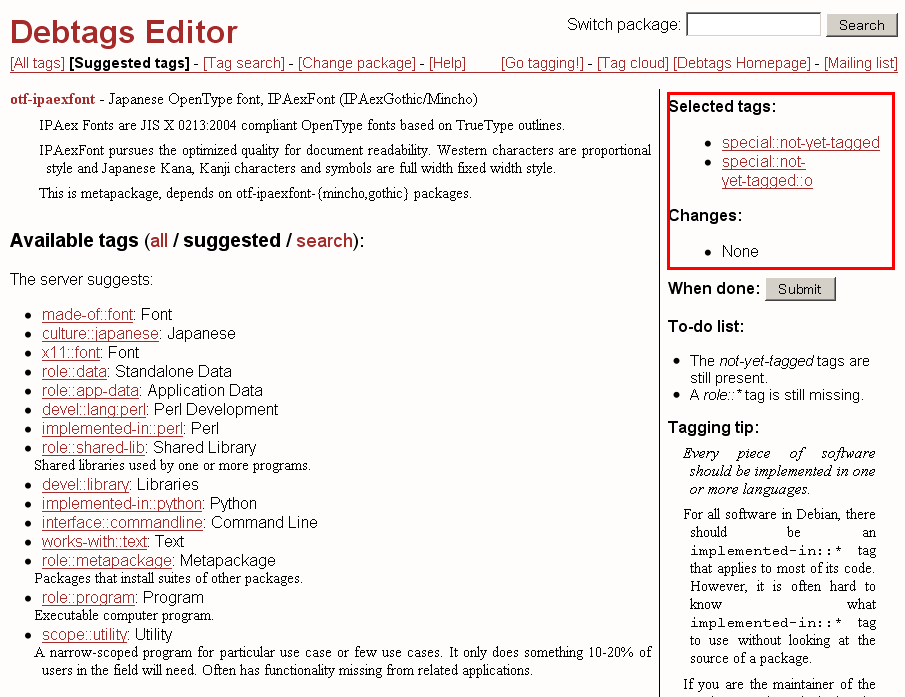
\includegraphics[height=0.5\hsize] {image201004/gotagging02.png}
 \caption{debtags $B%?%0IU$1(B web $B%$%s%?!<%U%'%$%9$NMM;R(B}
\label{fig:gotagging02}
\end{center}
\end{figure}

\begin{itemize}
 \item $BA*Br$7$?%Q%C%1!<%8$N@bL@!J2hLL:8>e!K(B
 \item $BMxMQ2DG=$J%?%0$N6hJL!'(Ball$B!J$9$Y$F!K(B/ suggested $B!J$*$9$9$a!K(B/ search $B!J8!:w!K(B
 \item $B%?%0$N0lMw!J2hLL:82<!K(B
 \item $B4{$KIU$1$i$l$?!&IU$1$i$l$k%?%0!J2hLL1&!K(B
\end{itemize}

\clearpage

\subsection{$B=$@5$,I,MW$J%?%0(B}

$B$^$@%-%A%s$H%?%0IU$1$,$5$l$F$$$J$$%Q%C%1!<%8$K$O!"@V$$!_0u$H6&$K0J2<$N$h$&$JCm0U$,I=<($5$l$^$9!#(B
$B$3$3$+$i$^$:D>$7$F$$$/$3$H$r9M$($^$7$g$&!#(B

$B$=$l$>$l0J2<$N$h$&$J0UL#9g$$$G$9!#(B

   \begin{table}[h]
    \begin{center}
      {
        \begin{tabular}{l|l} \hline
                $BI=<($5$l$kCm0U(B & $B0UL#9g$$(B \\ \hline \hline
The not-yet-tagged tags are still present. & $B$3$N%Q%C%1!<%8$O$^$@%?%0IU$1$,=*$o$C$F$J$$$h!"$N%?%0$,;D$C$F$^$9!#(B \\
An implemented-in::* tag seems to be missing. & $B$3$N%=%U%H$O$[$2$[$28@8l$G<BAu$5$l$F$$$^$9!"$C$F%?%0IU$1$7$h$&$M(B \\
A role::* tag is still missing. & $B$3$N%=%U%H$NLr3d$r%?%0IU$1$;$h!J(Brole $B$OI,?\$G$9!K(B \\
A devel::lang:* tag seems to be missing. & $B$[$2$[$28@8l3+H/MQ$N%?%0$rIU$1$^$7$g$&(B \\
           \end{tabular}
        }
     \caption{$B%?%0IU$1$,$5$l$F$$$J$$%Q%C%1!<%8$NCm0U=q$-(B}
     \label{tagwarning}
    \end{center}
    \end{table}

$B$3$l$rF'$^$($F0J2<$N$h$&$J:n6H$r$7$^$9!#(B

\begin{itemize}
 \item $B$^$@%Q%C%1!<%8$r;XDj$7$F$$$J$$$J$i!"%Q%C%1!<%8L>$r%/%j%C%/(B
 \item $BDs<($5$l$k%?%0$d8!:w$7$?%?%0$r%/%j%C%/$7$FDI2C(B
 \item $BI,MW$J$$%?%0$,IU$1$i$l$F$$$k>l9g$O%/%j%C%/$7$F:o=|(B
 \item $B2hLL1&B&$N!V(BSelected tags:$B!W$H!V(BChanges:$B!W$r8+$F!"LdBj$,$J$$$3$H$r3NG'(B\fgref{fig:gotagging03}
 \item $B:G8e$K(B submit 
\end{itemize}


\begin{figure}[H]
\begin{center}
 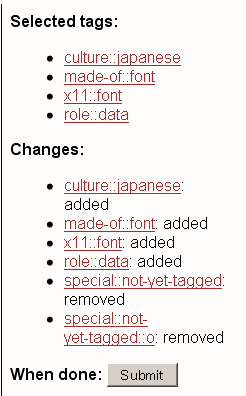
\includegraphics[height=0.5\hsize] {image201004/gotagging03.png}
 \caption{$B2hLL1&B&$N!V(BSelected tags:$B!W$H!V(BChanges:$B!W$r3NG'!*(B}
\label{fig:gotagging03}
\end{center}
\end{figure}


$B$3$l$@$1$G:n6H$O=*$o$j$G$9!#4JC1$G$9$M!*(B


\subsection{$B$I$s$J%?%0$,$"$k$N(B?}

$B%?%0IU$1<+BN$O4JC1$J$b$N$J$N$G!"%Q%C%1!<%8$KBP$7$FE,@Z$J%?%0$rIU$1$k$3$H$,4NMW$J$N$G$9$,!"(B
$B$9$Y$F$N%?%0$r3P$($k$3$H$OBgJQ$9$.$k$N$G$"$-$i$a$F!"(B
$B%5%$%H$,E,59Ds<($7$F$/$l$k$b$N$NCf$+$iA*Br$7$^$7$g$&!#(B
$B$"$H0l1~%,%$%I%i%$%s$b$"$j$^$9(B (\url{http://wiki.debian.org/DebTaggingGuidelines})

$B$G!":G=i$K!V?d>)!W%?%0$,I=<($5$l$F$$$^$9!#E,Ev$J$b$N$,$"$l$P$3$3$+$iA*$V$N$b$$$$$G$9$,!"$*4+$a$O(B
\begin{itemize}
 \item $BB>$N;w$?%Q%C%1!<%8$r8+$F$_$k(B $B"*(B $BF1$8%?%0;H$&(B
 \item all $B$rA*$s$G!"8!:wAk$+$i%-!<%o!<%I$G%?%0$r8!:w$9$k(B
\end{itemize}
$B$G$9!#(B


\subsection{$B$=$NB>5?LdE@(B}

\begin{itemize}
 \item $B0-0U$N$"$k%3%_%C%H$K$D$$$F$O!)(B spammer$B$J$I$OBg>fIW$+(B

        $B%3%_%C%H$5$l$?%?%0$K$D$$$F$O0l1~%V%i%&%6$N%/%C%-!<$,I3IU$1$i$l$F$$$F!"%l%S%e!<;~$K=EJu$7$F$$$kLOMM$G$9!#(B

 \item $B%3%_%C%H$OC/$G$b$G$-$k!)%l%S%e!<$O!)(B
 
        $B%l%S%e!<$9$k$K$O(B Alioth $B$N(B 'debtags' $B%0%k!<%W$K;22C$9$kI,MW$,$"$k$=$&$G$9!#(B
        $B$^$?>/$J$/$H$b(B Debian $B$r;H$C$F$$$J$$$H!"%l%S%e!<$NJ,N`$r$9$k:]!":Y$+$JE@$G$&$^$/H=CG$G$-$J$$$@$m$&$H$$$&$3$H$G$7$?!#(B
\end{itemize}


\subsection{$B:G8e$K(B}
Happy tagging!

% from debianmeetingresume200912-kansai.tex
\dancersection{Debian $B$r;H$C$FL{$7$`(B Open Street Map $BF~Lg(B}{$B$?$J$+$H$7$R$5(B}
\index{open street map}

\subsection{Open Street Map $B$r$4B8CN$G$9$+(B?}

\begin{figure*}[h!]
    \centering
    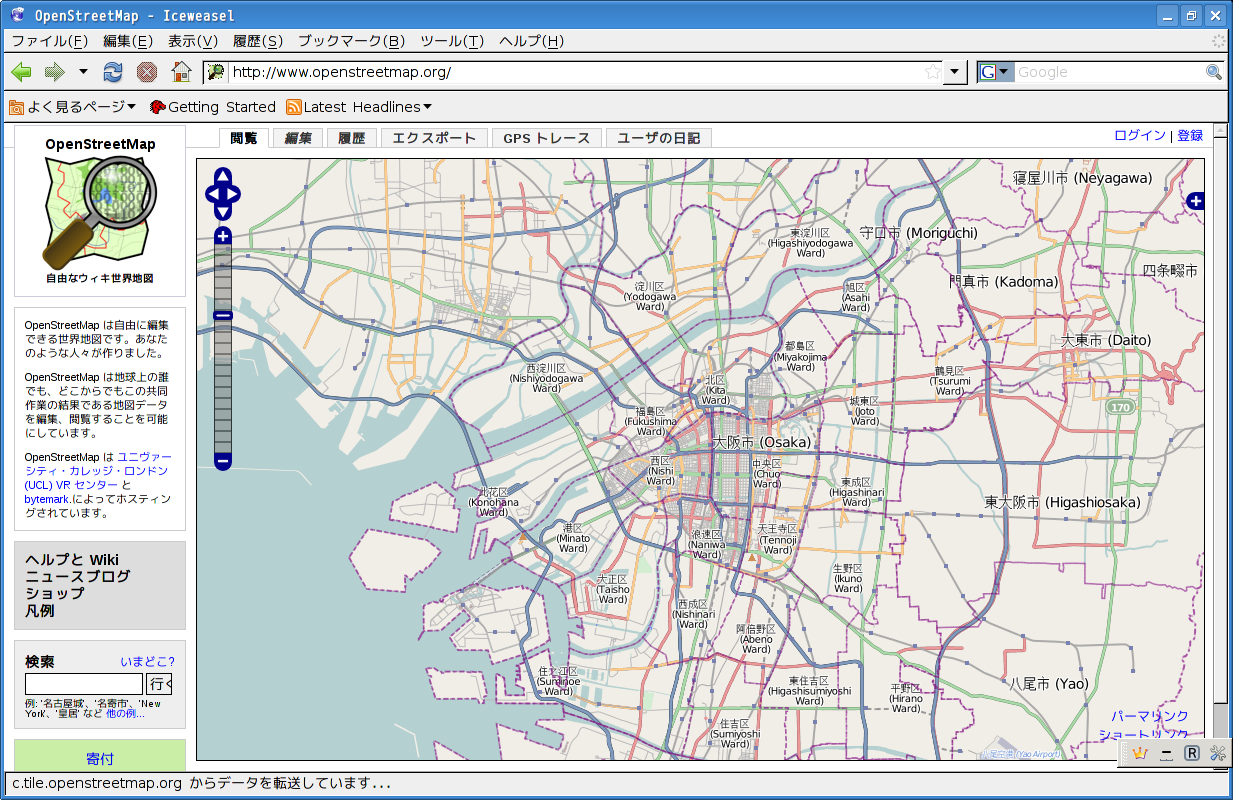
\includegraphics[scale=0.3]{image200912/debianosm1.png}
    \label{fig:debianosm1}
\end{figure*}

2009$BG/EY(B12$B7n$N(BDebian $BJY6/2q$N$*CN$i$;$G!"(B
\url{http://www.openstreetmap.org/} $B$K%"%/%;%9$7$F!"$*=;$^$$6aJU$NCO?^$r(B
$B8+$FD:$1$?$i$H0FFb$7$^$7$?!#(B

$B$4Mw$K$J$i$l$?3'$5$s!"46A[$O$$$+$,$G$7$g$&$+!#(B

$B!V$9$2$'!"AG@2$i$7$$!*!W(B

$B!V(BGoogle Map $B$NNw2AHG!)!W(B

$B!V(BDebian $B$H2?$N4X78$,$"$k$N$5!)!W(B

$B!!Ey$J$I!"?'!9$J46A[$,$"$k$H;W$$$^$9!#(B

$B:#2s$NJY6/2q$G$O!"(BDebian $B$N1~MQ$H$7$F!"(BDebian $B$r;H$C$F!"$3$N(B
OpenStreetMap($B0J9_!"(BOSM $B$HI=5-(B)$B$K$D$$$F!"0l=o$KJY6/$7$F$$$-$^$7$g$&!#(B

\subsection{$BLH@U(B}
\begin{itemize}
 \item $B$3$N%F%-%9%H$O!"$?$J$+$H$7$R$5(B(tosihisa@netfort.gr.jp)$B$,=q$$$?$b$N$G$9!#(B
 \item $B$3$N%F%-%9%H$K$O!"4V0c$$$,$"$k$+$b$7$l$^$;$s!#(B
 \item $B5-:\FbMF$O!"$G$-$k$@$1:G?7(B(2009$BG/(B12$B7n(B)$B$N;v>p$K$"$o$;$F5-:\$7$?$D$b$j$G$9$,!";~4V$N7P2a$GFbMF$,JQ2=$9$k>l9g$,$"$j$^$9!#(B
\end{itemize}

\subsection{OpenStreetMap(OSM) $B$C$F2?$G$9$+!)(B}
\url{http://wiki.openstreetmap.org/wiki/Ja:Main_Page} $B$+$i$N0zMQ$G$9!#(B

\begin{quotation}
OpenStreetMap$B$OF;O)CO?^$J$I$NCOM}>pJs%G!<%?$rC/$G$bMxMQ$G$-$k$h$&!"%U%j!<(B
$B$NCOM}>pJs%G!<%?$r:n@.$9$k$3$H$rL\E*$H$7$?%W%m%8%'%/%H$G$9!#<+M3$K;H$($k(B
$B$H;W$C$F$$$kCO?^$NB?$/$,<B$OK!E*!&5;=QE*$KLdBj$,$"$j!"?M!9$,%/%j%(%$%F%#(B
$B%V$K!"@8;:E*$K!"$"$k$$$O:#$^$GM=4|$7$J$+$C$?J}K!$G$=$l$r(B $BMxMQ$9$k;v$rK8$2(B
$B$F$$$k$?$a!"$3$N%W%m%8%'%/%H$O3+;O$5$l$^$7$?!#(B
\end{quotation}

\subsection{Debian $B$H(B OSM}

$B:#2s$N4X@>(B Debian $BJY6/2q$O!"=>Mh$N%F!<%^$H$O0[$J$j!"0[?'$G$b$"$j$^$9!#(B
$B!V(BOSM $B$C$F!"(BDebian $B$H2?$+4X78$"$k$N!)!W$H8@$o$l$k$H!"3N$+$K6/$$4X78!D(B
$B$O$"$j$^$;$s!#(B

$B$7$+$7!"(BDebian $B$H(B OSM $B$rAH$_9g$o$;$k;v$G!"(B

\begin{center}
 \textbf{{\large$B!V<+M3EY$N9b$$!WCO?^%=%U%H4D6-(B} }
\end{center}

$B$,<B8=$G$-$^$9!#$3$l$O!"2h4|E*$J;v$@$HI.<T$O9M$($F$$$^$9!#(B

Debian $B$G!"$I$l$@$1AG@2$i$7$$CO?^%=%U%H$,(B .deb $B$K$J$C$F(B apt $B$GF@$i(B
$B$l$k$H$7$F$b!"CO?^%G!<%?$,L5$1$l$PL%NO$r7g$-$^$9!#(B

Debian $B$r;O$a$?$H$7$?(B Linux $B%G%#%9%H%j%S%e!<%7%g%s$O!"!V<+M3$K;H$&(B
$B;v$,=PMh$k%3%s%T%e!<%?%=%U%H%&%'%"4D6-!W$r<B8=$G$-$k$b$N$G$9$,!"$=$l$H(B
OSM $B$H$rAH$_9g$o$;$k;v$G!"<+M3$K;H$&;v$,=PMh$k%3%s%T%e!<%?%=%U%H%&%'%"4D(B
$B6-$NCf$K!"!VCO?^$N1\Mw!W$r4^$a$k;v$,=PMh$^$9!#(B

Debian $B$b$=$&$G$"$k$h$&$K!"(BOSM $B$b$^$?!"!V0lIt$NFC8"3,5i!W$N$b$N$G(B
$B$O$"$j$^$;$s!#K>$a$P!"C/$G$b$,<+M3$K;H$&;v$,=PMh$^$9!#(B
OSM $B$O!";H$&$K$O0l6lO+$+$+$k;v$b$7$P$7$P$"$j$^$9$7!"CO?^<+?H!"F|K\9qFb$G(B
$B$O==J,$KB7$C$F$$$k$H$O8@$($J$$>u67$G$9!#(B

$B$7$+$7!"C/$G$b$,!"<+M3$K;H$($kCO?^%G!<%?$rDs6!$G$-$k;v$O!"(BDebian $B$,L\;X$9(B
$B%4!<%k$H=E$J$j$^$9!#(B

$B$^$?!"!VC1$K(B Debian $B$r;H$&!W$@$1$G$J$/!"(BDebian $B$N1~MQ;vNc$rA}$d$9;v$O!"(B
Debian $B%3%_%e%K%F%#$K<h$C$F$bM-1W$H9M$($F$$$^$9!#(B
Debian $B$O!"%5!<%P!"0eNE!"AH9~$_$J$I!"MM!9$JJ,Ln$G;H$o$l$F$$$^$9!#(B
$B$=$NCf$K!V<+M3$K;H$($kCO?^4D6-!W$r2C$($k;v$,=PMh$^$9!#(B

\subsection{OSM $B$N%i%$%;%s%9(B}

OSM $B$NCO?^%G!<%?$O!"(BCreative Commons Attribution-ShareAlike 2.0$B!"4JN,7O(B
$B$G=q$/$H(B CC BY-SA ($BI=<((B-$B7Q>5(B)$B$G$9!#(B
\footnote{\url{http://wiki.openstreetmap.org/wiki/Ja:OpenStreetMap_License}}

$B$J$*!"(BOSM $B$NCO?^%G!<%?$N%i%$%;%s%9$O!"(B2009$BG/(B12$B7n8=:_(B Open Database License (ODbL) $B$X$N0\9T$,8!F$$5$l$F$$$^$9!#(B
\footnote{\url{http://wiki.openstreetmap.org/wiki/Ja:Open_Database_License}}

12$B7n$N4X@>(B Debian $BJY6/2q<B;\:"$K$O!"$b$7$+$9$k$H%i%$%;%s%9$,JQ99$5$l$F$$$k$+$bCN$l$^$;$s!#(B

\textbf{{\large $B!v5^Jg!v(B} }

$BF|K\$N(B OSM $B%3%_%e%K%F%#$O!"(BODbL $B$K4X$9$k>pJs$rI,MW$H$7$F$$$^$9!#(B
ODbL $B$K>\$7$$(B($B=PMh$l$P(B)$BF|K\8l$N>pJs$,$"$j$^$7$?$i!"I.<T$^$G$*CN$i$;2<$5$$$^$9$H=u$+$j$^$9!#(B

ODbL $B$O!"F|K\$G$O$^$@G'CN$,Dc$$$?$a$+!"F|K\8l$N>pJs$,>/$J$/!"$I$NMM$J>pJs(B
$B$G$b9=$$$^$;$s$N$G!"I.<T$^$G$*CN$i$;2<$5$$$^$9$H=u$+$j$^$9!#(B

\subsection{OSM $B$NFCD'(B}

\subsubsection{OSM $B$NCO?^%G!<%?$O!"%S%C%H%^%C%W$G$O$J$/%Y%/%H%k%G!<%?(B}

OSM $B$NCO?^%G!<%?$O%Y%/%H%k%G!<%?$G$9!#(B
\url{http://www.openstreetmap.org/} $B$d!"(B\url{http://osm.jp/} $B$+$i;2>H$G$-(B
$B$kCO?^2hA|$O!"$=$N%Y%/%H%k%G!<%?$r%S%C%H%^%C%W%G!<%?$X%l%s%@%j%s%0$7$?$b(B
$B$N$G$9!#(B

$BCO?^%G!<%?$,%Y%/%H%k%G!<%?$J$N$G!"CO?^$NI=8=G=NO<+?H$O!"%S%C%H%^%C%W$KHf(B
$B$Y$k$HNt$j$^$9$,!"%Y%/%H%k%G!<%?$N>l9g!"3HBg!&=L>.$,<+M3$K9T$($k;v$H!"%k!<(B
$B%HC5:w$,2DG=$K$J$j$^$9!#(B

OpenStreetMap $B$NCO?^%G!<%?$rMQ$$$?%k!<%HC5:w%5!<%S%9$rDs6!$7$F$$$k%5%$%H(B
$B$N0l$D$K!"(BCloudMade $B$,$"$j$^$9!#(B
CloudMade $B$NCO?^%5%$%H(B (\url{http://maps.cloudmade.com/}) $B$K%"%/%;%9$7$F!"(B
$BBg:e(B($BG_ED(B)$B$+$i!"4X@>(B Debian $BJY6/2q$^$G$N%k!<%HC5:w7k2L$r(B\fgref{fig:debianosm2}$B$K<($7$^$9!#(B

\begin{figure}[h]
 \centering
 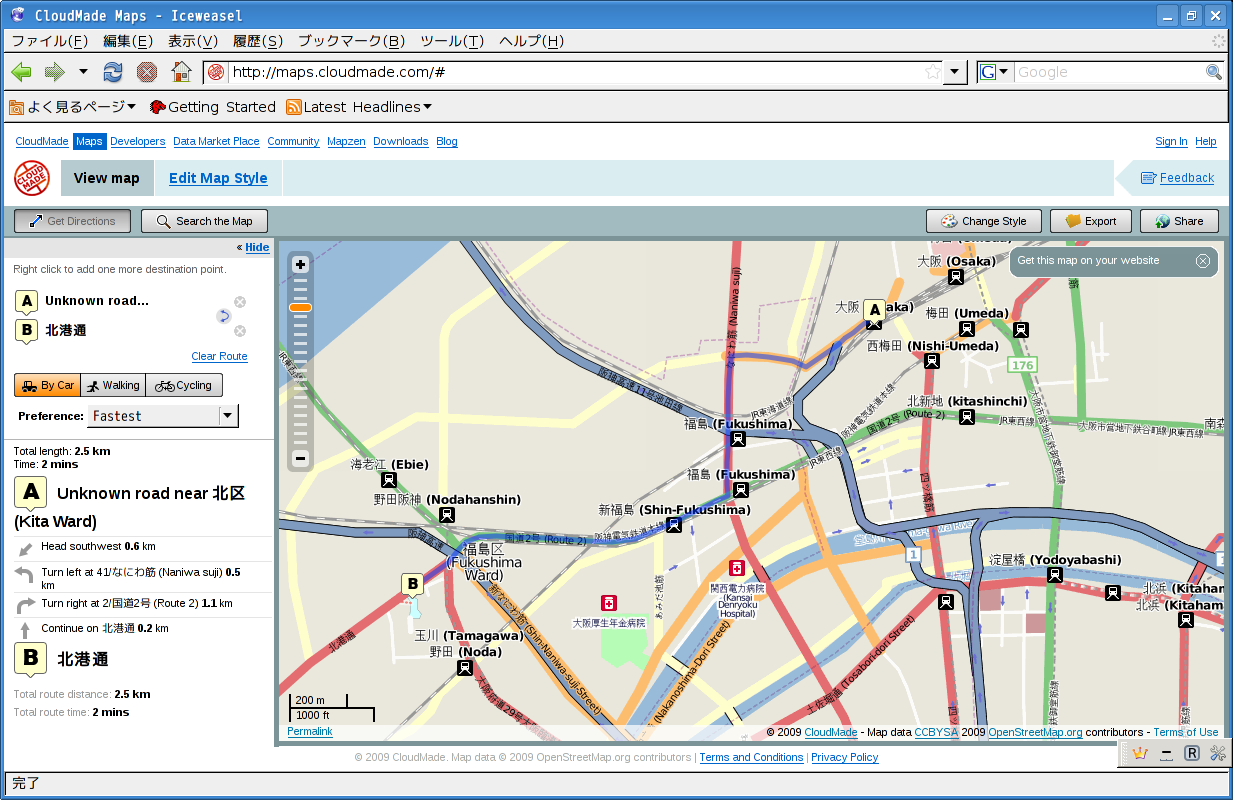
\includegraphics[scale=0.4]{image200912/debianosm2.png}
 \caption{CloudMade $B$K$h$k4X@>(B Debian $BJY6/2q$X$N%k!<%HC5:w?^(B}
 \label{fig:debianosm2}
\end{figure}

OSM $B$NCO?^%G!<%?<+?H$,$^$@$^$@ITB-$7$F$$$k;v$H!"CO?^%G!<%?$N@:EY$,B-$j$J(B
$B$$$N$G!"4|BT$7$?%k!<%HC5:w7k2L$K$O$^$@$J$i$J$$$+$bCN$l$^$;$s$,!"$3$NMM$J(B
$B%k!<%HC5:w$,9T$($k2DG=@-$r(B OpenStreetMap $B$O;}$C$F$$$^$9!#(B

\subsubsection{$BCO?^%G!<%?$N:n@.$O!"%"%+%&%s%HEPO?$5$($9$l$PC/$K$G$b2DG=(B}

\begin{wrapfigure}{r}{30zw}
 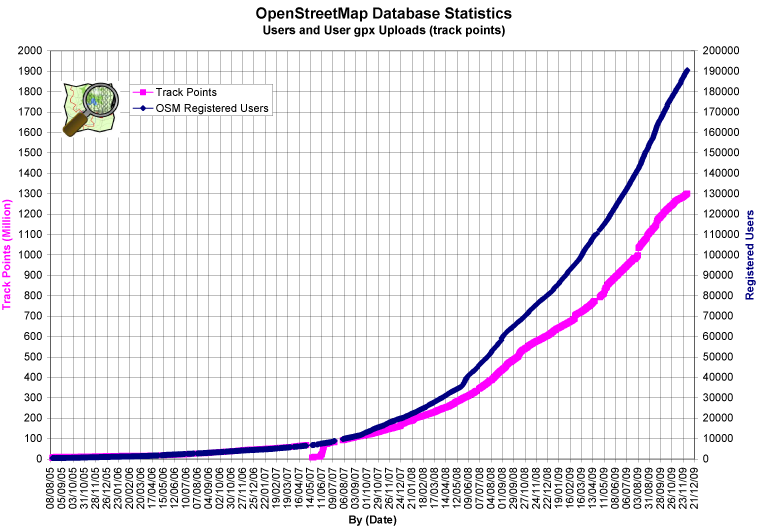
\includegraphics[scale=0.5]{image200912/debianosm3.png}
 \caption{OSM$BEPO?<T?t$H:n?^%G!<%?$N?d0\%0%i%U(B}
\end{wrapfigure}

OSM $B$NCO?^%G!<%?$N:n@.$O!"(BOSM $B$X$N%"%+%&%s%H$rEPO?$9$l$PC/$K$G$b:n@.!"JT(B
$B=8$,2DG=$G$9!#(B

2009$BG/(B5$B7n$K!"(BOSM $B%f!<%6?t$O(B 100,000 $B$r1[$($^$7$?!#1&$K!"$=$NEPO?<T?t$H(B
$B:n?^%G!<%?$N?d0\%0%i%U$r<($7$^$9!#(B
($B=PE5!'(B\url{http://www.opengeodata.org/2009/03/17/osm-passes-100000-users/})

\clearpage

\subsubsection{Wiki $B$N9M$(J}$r%Y!<%9$K$7$F$$$k(B}

$BCO?^%G!<%?$N:n@.$O!"(BWiki $B$N9M$(J}$,:,K\$K$"$j$^$9!#(BA $B$5$s$,:n?^$7$?%G!<%?(B
$B$r(B B $B$5$s$,=$@5$9$k;v$,2DG=$G$9!#(B
Wiki $B$N0-$$LL(B $B$$$o$f$k!V9S$i$7!WE*$J;v$b!"$d$m$&$H;W$($P=PMh$F$7$^$$$^$9(B
$B$7!"CO0h$K$h$C$F$O!VJT=89g@o!W$,$"$k$N$b;v<B$G$9!#(B

$B$7$+$7$J$,$i!"(BWiki $B%Y!<%9$G$"$k$N$G!"!V$h$jNI$$J}8~$K8~$+$C$F=$@5$9$k!W;v(B
$B$,2DG=$G$"$j!"Nc$($P0lJ}DL9T$NJ}8~$,5U$G$"$k;v$r8+$D$1$?>l9g!"%"%+%&%s%H(B
$B$r;}$C$F$$$l$P=$@5$9$k;v$,=PMh$^$9!#(B

\subsubsection{$BCO?^%G!<%?$O%*%U%i%$%s$G$bMxMQ$G$-$k(B}

GoogleMap $B$O<B$KJXMx$G$9$,!"4pK\$O%*%s%i%$%s!"MW$9$k$K%$%s%?!<%M%C%H$K7R(B
$B$,$C$F$$$k4D6-2<$G$"$k;v$,A0Ds$K$"$j$^$9!#(B
$B$^$?!"(BGoogleMap $B$,Ds6!$9$kCO?^$O!";vA0$K(B Google $B$N=qLL$KF10U$rF@$k;vL5$7(B
$B$KFH<+$N5;=Q$K$h$k%"%/%;%9$dCO?^$NJ#@=$O=PMh$^$;$s!#(B

$B=PE5!'(B
\begin{itemize}
 \item \url{http://www.google.co.jp/intl/ja_jp/help/terms_maps.html}
 \item \url{http://www.google.com/intl/ja_ALL/help/terms_local.html}
\end{itemize}

$B$3$l$O!"%*%U%i%$%sBP1~CO?^1\Mw%=%U%H$O!"(BGoogle Map $B$NCO?^%G!<%?$r=qLL$K$h(B
$B$kF10UL5$7$K;H$($J$$;v$r0UL#$7$^$9!#(B
$B%*%U%i%$%s$G$bCO?^$r1\Mw$G$-$k%=%U%H$K(B Mobile GMaps
(\url{http://www.mgmaps.com/}) $B$,$"$j$^$9!#$3$l$O%*%s%i%$%s$G$b%*%U%i%$%s$G$b;H(B
$BMQ$G$-$k(B PDA $B$d(B SmartPhone $B8~$1CO?^%=%U%H$G$9$,!">e5-$NM}M3$+$i!"$3$N%=%U(B
$B%H$O(B Google Map $B$NCO?^$KBP1~$7$F$$$^$;$s!#(B

$B8m2r$NL5$$MM$KIU$12C$($k$H!"I.<T$O(B GoogleMap $B$N$"$jJ}$OLdBj;k$7$F$$$^$;$s!#(B
GoogleMap $B$,Ds6!$9$k%5!<%S%9$O!"$3$l$i$rJd$&$K==J,$H9M$($F$$$^$9!#(B

$BBg;v$J;v$O!"%$%s%?!<%M%C%H$,$I$3$G$b0B2A$K;H$($kMM$K$J$C$?$H$O8@$(!"$=$l(B
$B$O!VA4@$3&$+$i8+$l$P$4$/0lIt!W$G$7$+L5$$$H8@$&;v$G$9!#(B
$BF|K\$G$b!";34V$NCO0h$K9T$/$H!"7HBS$b7w30$K$J$k>l9g$,$"$j$^$9!#(B

$B$3$NMM$J>l9g$G$b!"CO?^%G!<%?$r%*%U%i%$%s$G;}$C$F$*$1$P!"7w30$G$bCO?^$r1\(B
$BMw$G$-$^$9$7!"7wFb$G$b%Q%1%C%H2]6b$r5$$K$9$kI,MW$O$"$j$^$;$s!#(B

OSM $B$NCO?^%G!<%?$r%*%U%i%$%s$G8+$i$l$k%=%U%H$N0l$D$K!"(Bnavit
(\url{http://wiki.navit-project.org/index.php/OpenStreetMaps}) $B$,$"$j$^$9!#(B
navit $B$O8e$N>O$G>R2p$7$^$9!#(B

\subsection{($B:#$@$1$NL{$7$_$G$9$,(B)$BAv9T%m%0$K$J$j$^$9(B}

$BI.<T$O%P%$%/$K>h$j!"%"%A%3%A$K0\F0$9$k$N$,<qL#$G!"(BGPS $B$r;}$C$F=P$+$1$F%m(B
$B%0$r<h$C$F8e$GD/$a$?$j$7$^$9!#$=$N;~!"!VC1$K%m%0$r8+$k!W$@$1$G$O$J$/!"(B
$B!V$=$N%m%0$r85$KCO?^$r:n?^$9$k!W;v$,=PMh$l$P!"$5$i$K$h$jNI$$$H9M$($F$$$^(B
$B$9!#(B

$BI.<T$,(B OSM $B$KCO?^%G!<%?$r%3%_%C%H$7;O$a$?:"$O!"Bg:e$OKX$I2?$b$"$j$^$;$s$G(B
$B$7$?!#5-21$G$9$,!"L>?@$+:e?@9bB.$N0lIt$,$"$C$?DxEY$G$9!#$I$J$?$+!"Bg:e$r(B
$BDL2a$5$l$?J}$,:n?^$5$l$?$N$@$H;W$$$^$9!#(B

$BI.<T$O$^$:!"Bg:e$N%7%s%\%k8fF26Z$r:n?^$7$^$7$?!#B3$1$F!";M%D666Z$r:n?^$7(B
$B$^$7$?!#Ev;~$O!V9-Bg$JGrCO?^!W$G$7$?$N$G!"$I$3$rAv$C$F$b:n?^$G$-$^$7$?$,!"(B
$B:G6a$NBg:e$N(B OSM $BCO?^$NH/E8$OL\3P$7$/!">/$79M$($F%m%0$r<h$i$J$$$H!"C/$+$,(B
$B4{$K:n?^:Q$_$N=j$rAv$C$F$$$k$@$1$K$J$j$^$9!#(B

$B6a5&COJ}$G:G$b(B OSM $B$N:n?^$,?J$s$G$$$k$N$O!"<"2l8)D9IM;T$N(B OSM $BCO?^$H9M$((B
$B$F$$$^$9!#(B
$B<"2l8)D9IM;T$N(B OSM $BCO?^H/E8$OL\3P$7$$$b$N$G!"!V$h$/$>$3$3$^$G:n?^$7$?$b$N(B
$B$@$J$!!&!&!&!W$H46C2$9$k;v$7$-$j$G$9!#(B

$BI.<T$O!"!V<+M3$K;H$($kCO?^$r!Z;H$$$?$$![!W$H8@$&M}M3$G(B OSM $B$KCmL\$7;O$a$^(B
$B$7$?!#$,!"%_%$%i<h$j$,%_%$%i$H8@$&Lu$G$O$"$j$^$;$s$,!"L\E*$,!V<+M3$K;H$((B
$B$kCO?^$r!Z:n$k$3$H![!W$KJQ$C$F$-$F$$$k$N$b;v<B$G$9!#(B

\subsection{OSM $B$X$N%3%_%C%H$O!"CO0h<R2q$X$N9W8%$K$b$J$j$($^$9!#(B}

$BI.<T$O>o!9!";v(B OpenSource $B$N@.2L$O!"CO85<R2q$K$b$D$J$,$l$P$H9M$($F$$$^$9!#(B

$B%W%m%0%i%_%s%08@8l(B Ruby $B$O!"Eg:,8)$N(B IT $B$J$i$S$K(B OpenSource $BB%?J$KNI$$1F(B
$B6A$rM?$($?$H9M$($F$$$^$9!#(BOSM $B$O!"$=$l$HF1$88z2L$r;}$A$($k$H9M$($F$$$^$9!#(B

$B!VCO?^!W$H8@$&$N$O!"(BOpenSource $B%3%_%e%K%F%#$K8B$i$:!"C/$K$G$b0l1~$N6=L#$,(B
$B$"$j$^$9!#;d$NJl$O%3%s%T%e!<%?4D6-$HL51o$J@83h$rAw$j$D$E$1$F$$$^$9$,!"Jl(B
$B$O;3Jb$-$,<qL#$J$N$GCO?^D"$O;}$C$F$$$^$9!#(B

$B$^$?!"F|K\$OCO?L$,B?$$$N$G!"HrFq>l=j$X$NCO?^$r:\$;$?4GHD$rL\$K$9$k$H;W$$(B
$B$^$9!#(B
$BI.<T$O!"(BOSM $B$,CO?LEy$N:R32H/@8;~$KLr$KN)$DF|$,Mh$l$P$H9M$($F$$$^$9!#(B
$BCO?LEy$N:R32$G!"F;O)$,J,CG$5$l$?>l9g!"$I$3$+$i$I$3$^$G$,DL9TIT2D$J$N$+$I(B
$B$&$+$r!"?WB.$KH?1G$G$-$k;EAH$_$r!"(BOSM $B$O;}$C$F$$$k$H9M$($^$9!#(B

$B$^$?!";kNO$,<e$/!"CO?^$r8+$k;v$,=PMh$J$$>l9g$K$b!"(BOSM $B$NCO?^$r%Y!<%9$K(B
$B!V?(CO?^!W$r:n$C$F$_$?%1!<%9$,$"$j$^$9!#(B

$B8=:_$N(B OSM $B$NCO?^%G!<%?$O!"F|K\9qFb$G8+$l$P!"$^$@$^$@B-$j$J$$$N$,8=>u$G$9(B
$B$,!"!VCO?^!W$OKX$I$N?M$K$O!">/$J$+$i$:4X78$,$"$k$b$N$G$9$N$G!"(B

$B$3$NMM$K!"MM!9$J7A$G$N1~MQ$r(B OSM $B$O;}$C$F$$$^$9!#(B

\subsection{OSM$B$X$N;22C(B}

OSM$B$X$N;22C$O!"(B
\url{http://wiki.openstreetmap.org/wiki/Ja:Beginners_Guide}$B$r;29M$K$9$k$H(B
$BNI$$$G$7$g$&!#4pK\E*$K$O2<5-$N;v$r$7$F$$$-$^$9!#(B

\subsubsection{OSM$B%"%+%&%s%H$N:n@.(B($B=i$a$N(B1$B2s$@$1(B)}

\url{http://www.openstreetmap.org/create-account.html}$B$K%"%/%;%9$7$F!"(B
OSM$B%"%+%&%s%H$r:n@.$7$^$9!#F1;~$K!"(B
\url{http://wiki.openstreetmap.org/index.php?title=Special:UserLogin&type=signup&uselang=ja}
$B$K%"%/%;%9$7$F!"(BOSM $B$N(B Wiki $B%"%+%&%s%H$r:n@.$7$F$*$/$HNI$$$G$7$g$&!#(B

OSM$B$O!"CO?^%G!<%?$N%"%C%W%m!<%I$O!V(BOSM$B%"%+%&%s%H!W$rMQ$$$^$9$,!"$=$l0J30(B
$B$K$b(B OSM $B$N(B Wiki $B%Z!<%8(B(\url{http://wiki.openstreetmap.org/})$B$,$"$j$^$9$N(B
$B$G!"(BOSM$B$K4X$9$k>pJs8x3+$KMQ$$$k$HNI$$$G$7$g$&!#(B

$B%"%+%&%s%H$N:n@.$O=i$a$N(B1$B2s$@$1$G$9$,!"8e!9$N(BGPS$B%m%0$N%"%C%W%m!<%I$d:n?^$G$O(BOSM$B%"%+%&%s%H>pJs$,I,MW$G$9!#(B

OSM$B:n?^$NN.$l$r(B\fgref{fig:debianosm4}$B$K<($7$^$9!#(B

\begin{figure}[h]
 \centering
 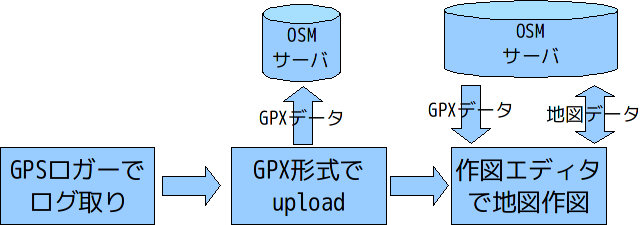
\includegraphics[scale=0.7]{image200912/debianosm4.png}
 \caption{OSM$B:n?^$NN.$l(B}
 \label{fig:debianosm4}
\end{figure}


\subsubsection{GPS$B%m%,!<$G%m%0<h$j(B}

GPS$B%m%,!<$r;}$C$F!"$^$@CO?^%G!<%?$NL5$$GrCO?^$N=j$K9T$-!"(BGPS $B%G!<%?$r%m%0(B
$B$7$F$$$-$^$9!#(B

$B!V%^%C%T%s%0%Q!<%F%#!W$H8@$&:E$7$,$"$j$^$9!#$3$l$O!"(BOSM$BF19%$N=8$^$j$G(BGPS
$BEy$r;}$C$F%m%0$r<h$k:E$7$G$9!#$3$N!V%^%C%T%s%0%Q!<%F%#!<!W$K;22C$9$k$N$b(B
$BNI$$$G$7$g$&!#(B

\subsubsection{GPS$B%m%0%G!<%?$r%"%C%W%m!<%I$9$k(B}

GPS$B%m%,!<$N%G!<%?$r(BGPX$B7A<0$K$7$F!"(BOSM$B%5!<%P$K%"%C%W%m!<%I$7$^$9!#(B

$B5;=QE*$K$O!"(BGPS$B%m%0%G!<%?$r%"%C%W%m!<%I$7$J$/$F$b:n?^$=$N$b$N$O2DG=$G$9$,!"!V(BGPS$B$r85$K$7$?F;$G$"$k;v!W$X$N:,5r$H$7$F!"(BGPS$B%m%0%G!<%?$O%"%C%W%m!<%I$7$F$*$$$?J}$,NI$$$G$7$g$&!#(B

\subsubsection{$BCO?^%G!<%?$r:n@.!"JT=8$9$k(B}

\begin{figure}[h]
 \centering
 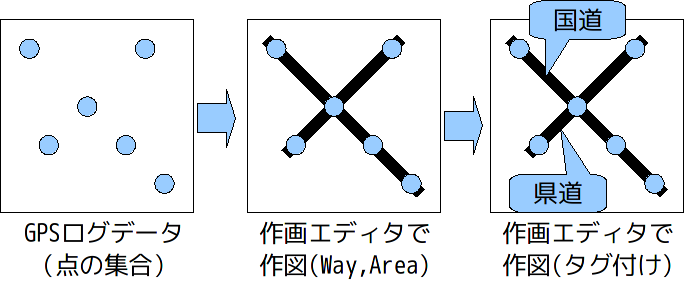
\includegraphics[scale=0.7]{image200912/debianosm5.png}
 \caption{$B:n?^%$%a!<%8(B}
 \label{fig:debianosm5}
\end{figure}

GPS$B%m%0%G!<%?$r85$K!"(BOSM$B:n2h%(%G%#%?$r;H$C$F!"<B:]$K:n?^$7$F$$$-$^$9!#(B

GPS$B%m%0%G!<%?$O!"E@%G!<%?$N=89g$G$9$N$G!"$=$l$r(BOSM$B:n?^%(%G%#%?$G7R$$$G9T$-!"@~$K$7$F$$$-$^$9!#(B

$B<!$K!"$=$N@~%G!<%?$,9qF;$J$N$+!"8)F;$J$N$+!"0lJ}DL9T$+$I$&$+$N>pJs$rIU2C$7$F$$$-$^$9!#$3$l$r!"!V%?%0IU$1!W$H8@$$$^$9!#(B
$B:n?^$N%$%a!<%8$r(B\fgref{fig:debianosm5}$B$K<($7$^$9!#(B

\subsubsection{$B%^%C%W$rIA2h$9$k!*(B }
$B=PMh>e$,$C$?CO?^$r8+$F$_$^$7$g$&!*(B
$BCO?^$N%l%s%@%j%s%0$K$O>/$7;~4V$,$+$+$j$^$9$,!"Aa$1$l$P(B1$B;~4V0L$G%l%s%@%j%s%0$5$l$^$9!#(B

\subsection{OSM $B$X;22C$9$k$K$O!"(BGPS$B%m%,!<$OIT2D7g$J$N!)(B}

GPS$B%m%,!<$,L5$$$+$i$H8@$C$F!"(BOSM$B$K;22C$G$-$J$$;v$O$"$j$^$;$s!#(BGPS$B%m%,!<$,L5$/$F$b!"2<5-$N7A$G(BOSM$B$X%3%_%C%H$G$-$^$9!#(B

\begin{itemize}
 \item $B;H$C$F$_$k!#(B\\
OSM$B$OCO?^%G!<%?$G$9$N$G!"<B:]$K$=$l$,8=<B$H$"$C$F$$$k$+$,=EMW$G$9!#$H$K$b$+$/$K$b!"(BOSM$B$r;H$C$F$_$F2<$5$$!#(BDebian $B$HF1MM$K!"!V$=$l$r;H$&!W$@$1$G$b!"9W8%$H$7$F=<J,$J$N$G$9!#(B
 \item $B4V0c$$$r=$@5$9$k!#(B\\
OSM$B$N:n?^$O!"$G$-$k$@$1@5$7$/$J$k$h$&$K:n?^$,?J$s$G$$$^$9$,!"Nc$($P0lJ}DL9T$NJ}8~$,5U$@$C$?$j!"9qF;!?8)F;$NHV9f$,4V0c$C$F$$$k>l9g$b$"$j$^$9!#(B
$B$3$NMM$J>l9g!":n2h%(%G%#%?$G(BOSM$B%G!<%?$r%@%&%s%m!<%I$G$-$^$9$N$G!"4V0c$$$N$"$kItJ,$r%@%&%s%m!<%I$7$F=$@5$7$F%"%C%W%m!<%I$9$l$P!"4V0c$$$,=$@5$G$-$^$9!#(B
\end{itemize}

\subsection{Debian$B$G;H$($k(B OSM (GIS) $B4XO"%=%U%H(B}
$B!!(BDebian $B$O!"%a%s%F%J$N?TNO$K$h$jK-IY$J%P%$%J%j%Q%C%1!<%8$r;H$&;v$,$G$-$^$9$,!"(B
$B!!(BOSM $B4XO"$GMxMQ$G$-$k%=%U%H%&%'%"$r2<5-$K<($7$^$9!#$b$A$m$s!"$3$l$@$1$G$O$"$j$^$;$s!#(B
$B!!;d8+$G$9$,!"(BGPS $B$r07$&%=%U%H$O!"(BWindows $B$h$j$b(B Debian$B$NJ}$,B?4t$KEO$C$F$$$k$H46$8$F$$$^$9!#(B

\subsubsection{gpsd}

\begin{commandline}
# apt-get install gpsd
\end{commandline}

gpsd $B$O!"(BOSM$B$G$OI,?\$G$OL5$$$N$G$9$,!"(BDebian $B$d(B Linux $B$G(BGPS$B%G!<%?$r<u?.$9$k:]$K$[$\I8=`$H$7$F;H$o$l$F$$$k$N$G>R2p$7$^$9!#(B
$B$3$N%=%U%H$O!"(BGPS $B<u?.5!$H(B PC $B$r@\B3$7!"(BNMEA-0183 $B%;%s%F%s%9$^$?$O(B GPS $B$NFH<+%W%m%H%3%k$HDL?.$7!"8=:_$N0^EY7PEY!"(BUTC $B;~4V$r=hM}$7$^$9!#(B

Debian $B$GF0:n$9$kCO?^4XO"$N%=%U%H$O!"(BGPS $B<u?.5!$HD>@\DL?.$;$:!"(Bgpsd $B$r7PM3$7$F0^EY7PEY$N>pJs$rF@$k$b$N$,B?$$$G$9!#(B
gpsd $B$r7PM3$5$;$k;v$G!"(BGPS $B<u?.5!0l$D$KBP$7!"J#?t$N(B(GPS $B$rI,MW$H$9$k(B)$B%=(B
$B%U%H$,;H$($k$h$&$K$J$j$^$9(B(\fgref{fig:debianosm6})$B!#(B

\begin{figure}[h]
 \centering
 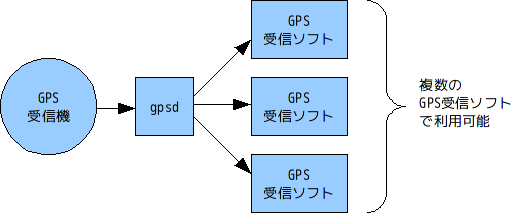
\includegraphics[scale=0.9]{image200912/debianosm6.png}
 \caption{gpsd$B$NF0:n%$%a!<%8(B}
 \label{fig:debianosm6}
\end{figure}

$B$^$?!"(Bgpsd $B$O!"(BNTP $B%5!<%P8~$1$N;~9o8;$H$7$F$b5!G=$7$^$9!#(BNTP(ntpd) $B$H$O!"6&M-%a%b%j%I%i%$%P$r2p$7$F9T$$$^$9!#$?$@$7!"(Bgpsd $B$r(B NTP $B%5!<%P8~$1$N;~9o8;$K$7$F$b!"(BNTP $B3,AX$N(B Stratum 1 $B$N@:EY$K$J$k$o$1$G$O$"$j$^$;$s!#$3$l$O!"(Bgpsd $B$,;~9o>pJs$r<u?.$9$k;~!"6&M-%a%b%j$K=q$-9~$`$H$-$K!V$f$i$.!W$,@8$8$k$+$i$G$9!#(B

Debian$B$H(B OSM $B$+$i$O>/$730$l$^$9$,!"$b$7!"(BGPS $B$r;~9o8;$H$7$F(B Stratum 1 $BAjEv$N(B NTP $B%5!<%P$r:n$k$J$i$P!"(B"1PPS (one pulse per second)" $B=PNO$D$-(B GPS $B$,I,MW$K$J$j$^$9!#(B

1PPS $B$H$O!"!V@53N$K#1IC$N%Q%k%9!W$rH/@8$9$k$b$N$G!"$3$N%Q%k%9$r(B Linux $B%+!<%M%k$GJa$^$($k;v$G!";~9o$N$f$i$.$r>/$J$/$7$^$9!#(B

\subsubsection{gpsbabel}

\begin{commandline}
# apt-get install gpsbabel
\end{commandline}

gpsbabel $B$O!"MM!9$J(B GPS $B%G!<%?$N7A<0$rJQ49$9$k%=%U%H$G$9!#(B

GPS $B%G!<%?$N!V4pK\E*$J;EMM!W$H$7$F$O!"(BNMEA-0183 $B%;%s%F%s%9$,$=$N4pK\$J$N(B
$B$G$9$,!"(BGPS $B<u?.5!%Y%s%@!<$O!"FH<+%U%)!<%^%C%H$G%G!<%?$rJ]B8$9$k>l9g$,$"(B
$B$j$^$9!#$=$l$OMM!9$J(BGPS$B%Y%s%@!<$+$i!"MM!9$J%G!<%?7A<0$,$"$j$^$9!#(BGoogle
Earth $B$N(B $B!H(B.kml$B!I7A<0$b!"$=$N(BGPS$B%m%0$NJ]B87A<0$N0l$D$G$9!#(B

gpsbabel $B$O!"$=$N(B GPS $B%G!<%?7A<0$rJQ49$9$k%=%U%H$G$9!#(B

OSM$B$,:NMQ$7$F$$$k(BGPS$B%m%07A<0$O!"(B<time>$B%?%0IU$-(BGPX$B7A<0$N$_$G$9$N$G!"$b$7(B
GPS$B<u?.5!!"$"$k$$$OIUB0%=%U%H$,(B<time>$B%?%0IU$-(BGPX$B7A<0$KBP1~$7$F$$$J$$>l9g!"(B
gpsbabel$B$GJQ49$7$J$1$l$P$J$i$J$$>l9g$,$"$j$^$9!#(B

$B;29M$K!"(BNMEA-0183 $B%;%s%F%s%9$N(BGPS$B%m%0%G!<%?$r(B GPX $B$KJQ49$9$k$K$O!"2<5-$N(B
$BMM$K<B9T$7$^$9!#(B

\begin{commandline}
$ gpsbabel -w -r -t -i nmea -f {nmea-log-file} -o gpx -F {GPX_DATA}.gpx
\end{commandline}

\clearpage

\subsubsection{Merkaartor ($BH/2;$O(B"$B%a%k%+%H%k(B"$B$G$9(B)}

$B!V(Bdeb \url{http://www.backports.org/debian} lenny-backports main contrib non-free$B!W$r!"(B/etc/apt/sources.list$B$KDI2C$7$^$9!#(B

\begin{commandline}
# apt-get update
# apt-get -t lenny-backports install merkaartor
\end{commandline}

\begin{wrapfigure}{l}{25.5zw}
 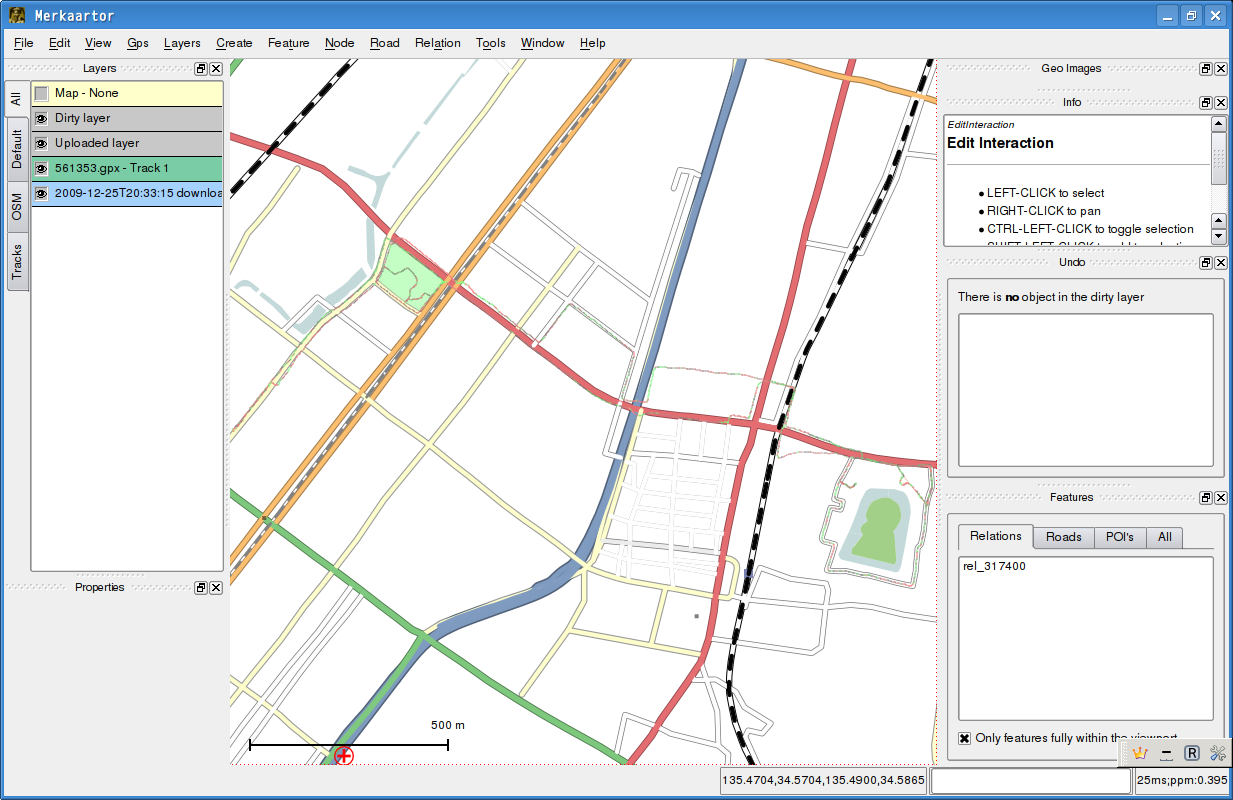
\includegraphics[scale=0.28]{image200912/debianosm7.png}
 \caption{Merkaartor$B%$%a!<%8(B}
 \label{fig:debianosm7}
\end{wrapfigure}

$B!!(BMerkaartor(\fgref{fig:debianosm7} $B$O!"(BOSM $B$N:n?^%=%U%H$G$9!#(B
$B!!(BOSM $B8~$1$N:n?^%=%U%H$O!"Bg$-$/#3$D$"$j$^$9!#(B

\begin{enumerate}
 \item Potlatch \\
Potlatch $B$O!"%U%i%C%7%e%Y!<%9$N:n?^%=%U%H$G!"(BWeb $B%V%i%&%6$,$"$l$P;H$&;v$,(B
$B=PMh$^$9!#(B
 \item JOSM \\
JOSM $B$O!"(BJava $B$G=q$+$l$?:n?^%=%U%H$GB?5!G=$G$9!#(BJava $BHG$J$N$G!"(BDebian $B$G(B
$B$b(B Windows $B$G$bF0$-$^$9!#(B
 \item Merkaartor
Merkaartor $B$O!"(BQt $B%i%$%V%i%j$r;H$C$F=q$+$l$?:n?^%=%U%H$G$9!#(B
JOSM $B$HF1$8$/(B Debian $B$G$b(B Windows $B$G$bF0$-$^$9!#(B
\end{enumerate}

$B$I$l$,$*>)$a$+!"$3$l$O#3$D$H$b<+M3$K;H$($k%=%U%H$G$9$N$G!"#3$D;n$7$F0lHV(B
$B<+J,$K9g$&$b$N$rA*$s$G2<$5$$!#0l35$K$I$l$,NI$$!&0-$$$H8@$&$N$O$"$j$^$;$s!#(B
$B$?$@!";d8+$G$9$,!"(BMerkaartor $B$OB?5!G=$GL5$$J,!"=i?4<T$K$H$C$F$O$+$($C$FJ,(B
$B$+$j$d$9$$$H9M$($F$$$^$9!#(B

Debian lenny $B$KF~$C$F$$$k(B Merkaartor $B$O>/$7%P!<%8%g%s$,8E$/!"(BDebian
Backports$B%5%$%H(B(\url{http://www.backports.org/}) $B$+$i!"=PMh$k$@$1?7$7$$(B
Merkaartor $B$r%$%s%9%H!<%k$9$k$HNI$$$G$7$g$&!#(B

\subsubsection{navit}

$B!V(Bdeb \url{http://navit.latouche.info/debian} lenny main$B!W$r!"(B/etc/apt/sources.list$B$KDI2C$7$^$9!#(B

\begin{commandline}
# gpg --recv-keys CB229096
# gpg --export -a CB229096 | apt-key add -
# apt-get update
# apt-get install navit
\end{commandline}

\begin{wrapfigure}{r}{23zw}
 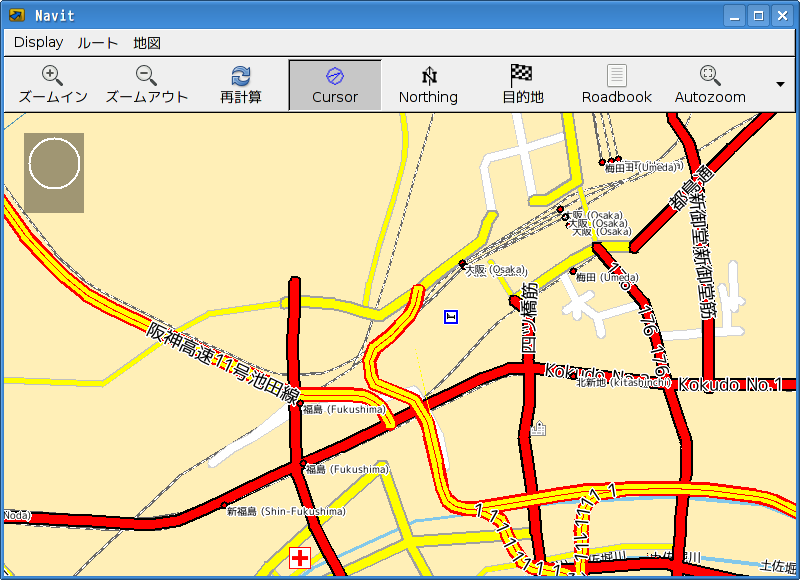
\includegraphics[scale=0.38]{image200912/debianosm8.png}
 \caption{navit$B%$%a!<%8(B}
 \label{fig:debianosm8}
\end{wrapfigure}

navit(\fgref{fig:debianosm8}) $B$O!"(BOSM $BCO?^%G!<%?$KBP1~$7$?CO?^I=<(%=%U%H$G$9!#(Bgpsd $B$,I,MW$G!"(B
gpsd $B$+$i8=:_$N0^EY7PEY$r<hF@$7!"(BOSM $BCO?^%G!<%?$H=E$M9g$o$;I=<($9$k;v$,=P(B
$BMh$^$9!#(B
navit $B$O(B OSM $BCO?^%G!<%?$r;vA0$K<h$j9~$`J}K!$G$9$N$G!"%M%C%H$,;H$($J$$%*%U(B
$B%i%$%s4D6-2<$G$bCO?^$r8+$k;v$,=PMh$^$9!#(B

$BI.<T$O(B Debian Lenny $B$r%$%s%9%H!<%k$7$?(B EeePC $B$K!"(Bgpsd $B$H(B navit $B$r%$%s%9%H!<(B
$B%k$7!"Bg:e$+$i?73c$^$G;H$C$F$_$?$3$H$,$"$j$^$9!#(B
$B<B:]$NAv9T$O!"KX$I$,9bB.F;O)$G$9$N$G!"%J%S$H8@$&$[$I$N$b$N$O$"$j$^$;$s$G(B
$B$7$?$,!";d$,G04j$H$7$F$$$?!"!V<+M3$J(B OS $B$G!"<+M3$J%=%U%H$G!"<+M3$JCO?^%G!<(B
$B%?$G%J%S$r$9$k!W$H8@$&;v$,C#@.$G$-$?=V4V$G$7$?!#(B

$BI.<T$O$^$@$^$@!"(BDebian $B$O=i?4<T$N0h$r=P$^$;$s!#$b$7(B Debian $B$K$"$k%Q%C%1!<%8$G!"NI$$$b$N$,$"$j$^$7$?$i>R2p2<$5$$!#(B

\subsection{$BI.<T$N(B GPS $B%m%05!4o(B}

$BI.<T$O!"<g$K(B2$BBf$N(B GPS $B<u?.5!$r;H$C$F%m%0$r<h$C$F$$$^$9!#(B

\subsubsection{GT-31}

GT-31 $B$O!">.7?KI?e$N(B GPS $B%m%,!<$G!"%P%$%/$K<h$jIU$1$k$3$H$,=PMh$^$9!#(B

GT-31 $B$NNI$$=j$O!"(BGPS $B%m%0$r(B SD $B%+!<%I$KJ]B8$9$k;v$,=PMh$k$N$G!"5-O?MFNL(B
$B$,(B SD $B%+!<%I$NMFNL<!Bh$GBg$-$/=PMh$kE@$G$9!#$^$?!"(BIPX7$BAjEv$NKI?e@-G=$,$"(B
$B$j$^$9!#(BIPX7 $BAjEv$NKI?e5!G=$H$O!"(B1m $B$N?eCf$K!"(B30$BJ,4VD@$s$G$$$F$bFbIt$K?e(B
$B$,F~$i$J$$9=B$$r;X$7$^$9!#(B

$BI.<T$O(B GT-31 $B$N(B SD$B%+!<%I$K!"(BNMEA-0183 $B$N7A<0$GJ]B8$7$F$$$^$9!#(B

\subsubsection{HI-406BT}

GT-31 $B$HJ;MQ$7$F!"(BHI-406BT $B$b;H$C$F$$$^$9!#(B

HI-406BT $B$O!"=c?h$J(B GPS $B<u?.5!$G$"$j!"$3$N5!4o<+?H$K%m%05!G=$O$"$j$^$;$s!#(B
HI-406BT $B$O(B Bluetooth $B%$%s%?!<%U%'!<%9$J$N$G!"I.<T$O(B Bluetooth $BIU$-$N(B
PDA $B$d(B PC $B$K!"$3$l$b(B NMEA-0183 $B$N7A<0$GJ]B8$9$k$h$&$K$7$F$$$^$9!#(B

\subsubsection{HOLUX m-241}
HOLUX m-241 $B$O!"C1(B3$B4%EECS0l$D$GF0:n$9$k>.7?(B GPS $B%m%,!<$G$9!#(B

$B>.7?$G$"$j$J$,$i!"%m%,!<$H$7$F$N5-O?MFNL$,Bg$-$/!"(B130,000$BE@$N%m%0$,2DG=$G(B
$B$9!#2C$($F(B Bluetooth $B$KBP1~$7$F$$$^$9!#I.<T$,(B OSM $B$K:n?^$7;O$a$?:"$O!"$3(B
$B$N(B m-241 $B$G%m%0$r<h$C$F$$$^$7$?!#(B
$B;DG0$J;v$K!"I.<T$N(B m-241 $B$O2u$l$F$7$^$$!":#$O(B GT-31 $B$H(B HI-406BT $B$rJ;MQ$7(B
$B$F$$$^$9!#(B

GPS $B$O!"M>M5$,$"$l$P(B2$BBfM_$7$$$G$9!#GrCO?^$r:n?^$9$k$H$-$O!"$d$O$j(BGPS$B%m%0(B
$B$+$i:n?^$7$^$9$N$G!"%m%0<h$jK:$l$O$+$J$j<d$7$$;v$K$J$j$^$9!#(B

GT-31 $B$O!"(BGPS $B%m%0$7$J$$!#$H8@$&A*Br;h$,L5$/!">o$K%m%0$7$^$9!#(Bm-241 $B$O!"(B
$B%\%?%s$N%H%0%k$G%m%0$9$k!&$7$J$$$rA*Br$G$-$^$9$,!"$D$$$&$C$+$jK:$l$F$7$^(B
$B$&;v$,$"$j$^$9$N$G!"(BGPS $B%m%0$r<h$k!&<h$i$J$$$,A*Br$G$-$k(B GPS $B<u?.5!$r;H$&(B
$B>l9g!"(BGPS $B%m%0>uBV$,$9$0$K3NG'$G$-$k$b$N$rA*$V$HNI$$$G$7$g$&!#(B

\subsection{GPS$B%m%,!<A*$SJ}%N%&%O%&(B}

\subsubsection{DOP (Dilution of Precision - $B@:EYDc2<N((B) $B$,J,$+$k$b$N$rA*$\$&(B}

GPS $B%l%7!<%P$O!"!V(BGPS $B1R@1$+$i8=:_0LCV$r$b$i$&!W$N$G$O$J$/!"(BGPS $B1R@1$+$i(B
$B@53N$J;~9o$H(B GPS $B1R@1$N0\F0>pJs$r85$K!"!V(BGPS $B%l%7!<%P$,<+NO$G8=:_CO$r7W;;(B
$B$9$k!W;EAH$_$G$9!#(B

$B$=$N$?$a!"7W;;7k2L$+$i!"@:EY$,$I$l$/$i$$Dc2<$7$F$$$k$+$rH=CG$9$k;v$,=PMh$^$9!#(B
$B$3$l$O(B GPS $B1R@10l$D$+$i8=:_CO$rCN$k$N$G$O$J$/!":GDc#3$D$N(B GPS $B1R@1$+$i8=(B
$B:_CO$r7W;;$9$k$?$a$G$9!#(B

DOP $B$O!">.$5$1$l$P>.$5$$$[$I@:EY$,NI$$;v$r<($7$^$9!#$3$N(B DOP $B$O!"<u?.$7$?(B
($B7W;;$KA*Br$7$?(B)GPS $B1R@1$N$P$i$16q9g$K$h$j$^$9!#(BDOP $B$K$O!"?eJ?J}8~$N(B
HDOP$B!"?bD>J}8~$N(B VDOP $B!"0LCV$r<($9(B PDOP $B$,$"$j$^$9!#(B

$B2<5-$N%Z!<%8$K5-:\$,$"$j$^$9$,!"(BOSM $B$O!"(BPDOP $B$NCM$O(B 4 $B$h$j2<!"(B2 $B$h$j2<$J(B
$B$i$+$J$jNI$/8GDj$5$l$F$$$k$H$"$j$^$9!#(B

\url{http://wiki.openstreetmap.org/wiki/Ja:Recording_GPS_tracks}

$BI.<T<+?H!":n?^$N$?$a$K(B GPS $B%m%0$r<h$k;~$O!"(BDOP $BCM$K$OAjEv5$$r;H$C$F$$$^$9!#(B

GPS $B%m%,!<(B "GT-31" $B$O!"(BDOP $BCM$rI=<($9$k$3$H$,=PMh$^$9$N$G!"I.<T$,(B GPS $B%m(B
$B%0$r<h$k;~$O!"8=:_$N0^EY7PEY$h$j$b!"(BDOP $BCM$rI=<($5$;$k$h$&$K$7$F$$$^$9!#(B
DOP $B$r%m%0$9$k(B GPS $B%m%,!<$r;HMQ$7$?>l9g!"(BGPX $B%m%0$K$b(B DOP $B$r;D$9;v$,=PMh(B
$B$^$9$N$G!"(BJOSM $B$d(B Merkaartor $B$G$b;k3PE*$K3NG'$G$-$^$9!#(B

NMEA-0183 $B%;%s%F%s%9$N>l9g!"(BGSA $B%;%s%F%s%9$,$3$l$K$"$?$j$^$9!#(B

\subsubsection{$B30It%"%s%F%J$,IU$1$i$l$k$N$HIU$1$i$l$J$$$N$G$OBg0c$$(B}

GPS $B<u?.5!$K$O!"30It%"%s%F%J$r<h$jIU$1$k;v$,=PMh$k$b$N$,$"$j$^$9!#(B
$BI.<T$O(B "HI-406BT" $B$H8@$&(B Bluetooth GPS $B%l%7!<%P$b;H$&$N$G$9$,!"$3$l$K$O30(B
$BIt%"%s%F%J$r<h$jIU$1$k$3$H$,=PMh$^$9!#(B

$B30It%"%s%F%J$r<h$jIU$1$k$3$H$G!"(BGPS $B?.9f$N46EY$,>e$,$j!"@:EY$,8~>e$7$^$9!#(B
$B$^$?!"30It%"%s%F%J$O35$MKI?e7?$G$9$N$G!"30It%"%s%F%J$r<V$N20:,$K<h$jIU$1!"(B
$BE78u$K:81&$5$l$:$K%m%0$r<h$k;v$,=PMh$^$9!#(B

\subsubsection{$BB,0L@:EY$N8m:9(B}

$B:G6a$N(B GPS $B<u?.5!$O@:EY$,8~>e$7!"35$M!V(B10m 2drms$B!W$NHO0O$G$9!#(B
$B!V(B2drms$B!W$H8@$&$N$O!"$3$l$rH>7B$H$9$k1_Fb$K!"$*$h$=(B 95\% $B$NB,0LE@$,F~$k;v(B
$B$rI=$7$^$9!#(B
10m 2drms $B$J$i$P!"H>7B(B10m $B$N1_Fb$K(B 95\% $B$NB,0LE@$,F~$k;v$r<($7$^$9!#(B

$BH>7B(B10m $B$@$H!"CO?^$H$7$F;H$&$N$K8m:9$H$7$F$OBg$-$$$+$bCN$l$^$;$s$,!"(BDGPS
$B$@$H(B 5m 2drms $B$K$^$G8m:9$,>/$J$/$J$k$b$N$b$"$j$^$9!#(B
GPS $B<u?.5!$r9XF~$9$k;~$O!"$3$N(B 2drms $B$NCM$O3NG'$7$F$*$/$HNI$$$G$7$g$&!#(B

\subsubsection{$B%P%C%F%j!<$N;}$A$H7A>u(B}

$B#1;~4VDxEY$N%m%0$G$"$l$P$"$^$jLdBj$O$"$j$^$;$s$,!"%P%$%/%D!<%j%s%0Ey$G$[(B
$B$\#1F|>h$j$C$Q$J$7$G(B GPS $B%m%0$r<h$k>l9g!"(BGPS $B<u?.5!$N%P%C%F%j!<$b5$$K$J$j(B
$B$^$9!#(B

GPS $B<u?.5!$N%P%C%F%j!<$N;}$A$b$=$&$G$9$,!"%P%C%F%j!<$N7A<0!"Nc$($P4%EECS(B
$B$+@lMQEECS$+$b!"MxMQ7ABV$K1~$8$F9M$($kI,MW$,$"$j$^$9!#(B

$B:G6a$N8D?MMQ(B GPS $B<u?.5!$O!"(BUSB $B$G=<EE$G$-$k$b$N$,$"$j$^$9!#$3$l$H7HBS$N=<(B
$BEE4o$K$"$k$h$&$J!"4%EECS$NEENO$r(B USB $B$KJQ49$7$F=P$9=<EE4o$rJ;MQ$9$k;v$G!"(B
$B@lMQEECS$G$b%P%C%F%j!<$r5$$K$;$:$K;H$&;v$,=PMh$^$9!#(B

$B$;$C$+$/$N(B GPS $B<u?.5!$b!"%P%C%F%j!<$,43>e$,$k$H!"(Bmapper $B$K$7$F$_$k$H$H$F(B
$B$b<d$7$$;v$K$J$j$^$9$N$G!"%P%C%F%j!<$N;}$A$d!"7A>u$O3NG'$7$F$*$/$HNI$$$G(B
$B$7$g$&!#(B

\subsection{$B$*$o$j$K(B}
OpenStreetMap$B$O!"F|K\$G$O$^$@$^$@G'CN$NDc$$%W%m%8%'%/%H$G$9$,!"(BDebian
System $B$H$b==J,?FOB@-$N9b$$%W%m%8%'%/%H$G$9$N$G!"6=L#$r;}$C$FD:$1$?$J$i$&(B
$B$l$7$$$G$9!#(B

% from debianmeetingresume200912-kansai.tex
\dancersection{$B%O%s%I%a%$%I(BGPS$B%m%,!<$N9=C[(B}{$B$^$5(B}
\index{gps logger}

\subsection{$B$O$8$a$K(B}

$B$3$l$^$G(BDebian$B$N%$%s%9%H!<%k!"4D6-@0Hw!"%&%'%V%"%W%j%1!<%7%g%s$N%7%9%F%`(B
$B9=C[$r$9$k$J$I%7%9%F%`$r?($k$3$H$O$"$kDxEY7P83$7$?$b$N$N!"$*>.8/$$D"%5!<(B
$B%P$d!"(BGPS$B%m%,!<$J$I!"2?$i$+$N<BMQ$K$J$k$b$N$O$J$+$J$+$D$/$l$^$;$s$G$7$?!#(B

$B$=$3$G%W%m%0%i%`$N%9%-%k$rF@$k$?$a$N65:`$H$7$F!"(BGPS$B%m%,!<$r:n@.$7$?$N$G!"(B
$BJs9p$7$^$9!#(B

$B$3$l$+$i(BDebian$B$rL\;X$9?M$N6=L#$r<f$-!"<j$,$+$j$H$J$C$F>/$7$G$b$*Lr$KN)$F(B
$B$l$P9,$$$G$9!#(B

\subsection{GPS$B$H$O(B}
``Global Positioning System'' $B$O?t==8D$N1R@1$+$i$NEEGH$r<u?.$7$F8=:_0LCV$r3d$j=P$9%7%9%F%`$G$9!#(B

$B86M}Ey$O$$$m$s$J=q@R$d%$%s%?!<%M%C%H$K7G:\$5$l$F$$$k$h$&$G$9$N$G!"$3$3$G$O@bL@$r3d0&$7$^$9!#(B

\subsection{GPS$B%m%,!<$N%O!<%I9=@.(B}
$BI,MW$J%O!<%I9=@.$O0J2<$NDL$j$G$9!#(B

$B:#2s<B:]$K;HMQ$7$?%O!<%I$N35N,;EMM$O(BAppendix$B$r;2>H$7$F$/$@$5$$!#(B
\begin{center}
        \framebox[6.5zw]{$B%M%C%H%V%C%/(B}
        \hspace{1em}$\Longleftarrow$\hspace{1em}
        \framebox[7.5zw]{PS2-USB$BJQ49(B}
        \hspace{1em}$\Longleftarrow$\hspace{1em}
        \framebox[7.5zw]{GPS$B%l%7!<%P(B}        
\end{center}

\begin{enumerate}
 \item GPS$B%l%7!<%P(B \\
            GPS$B%"%s%F%J!"<u?.2sO)!"?.9fAw=P2sO)$+$i@.$j!"(B PS2$B%3%M%/%?$+$i%7%j%"%k$K%-%c%i%/%?J8;z$G(BGPS$B>pJs$,Aw=P$5$l$^$9!#(B
 \item PS2-USB$BJQ49(B \\
            GPS$B%l%7!<%P$+$i?.9fAw=PMQ$N%7%j%"%k%$%s%?%U%'!<%9$r(BUSB$B%$%s%?%U%'!<%9$KJQ49$9$k$?$a$N$b$N$G$9!#JQ49%1!<%V%k$K$J$C$F$$$^$9!#(B
 \item $B%M%C%H%V%C%/(B \\
            USB$B%$%s%?%U%'!<%9$G<u?.$7$?(BGPS$B>pJs$r<u$1<h$j!"%U%!%$%k$KN/$a9~$_$^$9!#$^$?!"(BGPS$B>pJs$r$$$m$$$m2C9)$7$F3Z$7$a$^$9!#(B
\end{enumerate}

\subsection{$B%M%C%H%V%C%/%;%C%H%"%C%W35MW(B}
$B%M%C%H%V%C%/9XF~D>8e$+$i(BGPS$B%m%,!<$r9=C[$9$k>l9g$K$D$$$F35MW$r@bL@$7$^$9!#(B

\begin{enumerate}
      \item Debian Base system$B$N%$%s%9%H!<%k(B \\
    Debian-netinst-iso$B$r;H$C$F(BBase system$B$r%$%s%9%H!<%k$7$^$9!#(B
      \item X Window System$B$N%$%s%9%H!<%k(B
      \item Gnome$B$N%$%s%9%H!<%k(B
      \item $BF|K\8lF~NO%7%9%F%`$N%$%s%9%H!<%k(B \\
    $B%W%m%0%i%`:n@.;~I,MW$G$9!#:#2s$O!"(B``uim-anthy'' $B$r%$%s%9%H!<%k$7$^$7$?!#(B
      \item NTP$B$N%$%s%9%H!<%k(B \\
    $B%7%9%F%`;~9o<+F0D4@0MQ$N%W%m%0%i%`$G$9!#(B
    $B:#2s$O(BGPS$B$r07$&$?$a!"FC$K%7%9%F%`;~9o$,Bg@Z$K$J$k$H;W$o$l$^$9!#(B
      \item $B%W%m%0%i%`8@8l$N%$%s%9%H!<%k(B \\
    GPS$B%m%,!<%"%W%j%1!<%7%g%s:n@.$KI,MW$G$9!#(B
    $B:#2s$O!"$H$C$D$-$d$9$/!"(BGUI$B$,$G$-!"(B
    $B%i%$%V%i%j$,K-IY$H8@$o$l$k(B ``Python'' $B!J%P%$%H%s(Bor $B%Q%$%=%s!)!K(B
    $B$rA*Br$7$^$7$?!#(B
    $B;d$K$H$C$F!"3N$+$K$H$C$D$-$d$9$$$G$9$,!"$=$l$J$j$K6lO+$7$^$7$?!#(B
    python$B$N$;$$$G$O$J$/!"%W%m%0%i%_%s%0$H$$$&$b$N<+BN!"(B
    $B;W$C$?$b$N$,$=$&4JC1$K$G$-$k$o$1$G$O$J$$$H$$$&$3$H$@$H;W$o$l$^$9!#(B
      \item Python library$B$N%$%s%9%H!<%k(B
    \begin{enumerate}
          \item PySerial \\
        $B%7%j%"%k%]!<%HF~=PNOMQ$N%W%m%0%i%`$G$9!#(B
          \item Python Tkinter \\
        GUI$B%W%m%0%i%_%s%0MQ$N$R$H$D$G$9!#(B
          \item datetime \\
        $B;~9o$r07$&$H$-;H$$$^$9!#(B
          \item os, os.path \\
        $B%U%!%$%k$N3+JD!"FI$_=q$-$9$k$H$-;H$$$^$9!#(B
          \item sys($B>l9g$K$h$C$F;HMQ(B) \\
        $B%3%^%s%I%Q%i%a!<%?$r<hF@$9$k$H$-;H$$$^$9!#(B
    \end{enumerate}
\end{enumerate}

\subsection{GPS$B%G!<%?=PNO7A<0(B}
$B:#2s;HMQ$7$?(BGPS$B%l%7!<%P$O(BNMEA0183$B$H$$$&%W%m%H%3%k$G$9!#(B
NMEA0183$B$G$O0J2<$N$h$&$J7A<0$J$I$G%G!<%?$,=PNO$5$l$^$9$,!"(B

\begin{description}
 \item[GLL] Geographic Position, Latitude and Longitude
 \item[GSA] GNSS DOP and Active Satellites
 \item[RMC] Recommended Minimum Specific GNSS Data
\end{description}

$B:#2s$O(B

\begin{description}
 \item[GGA] Global Positioning System Fix Data
\end{description}

$B$H$$$&7A<0$N$_MxMQ$7$^$7$?!#(B
\clearpage
GGA$B7A<0$N;EMM$O<!$NDL$j$G$9!#(B

\begin{commandline}
GGA,123519.00,4807.038247,N,01131.324523,E,1,08,0.9,545.42,M,46.93,M,5.0,1012*42
123519.00 	$B!a!!B,0L;~9o!J(BUTC$B!K!!(B12:35:19.00
4807.038247,N 	$B!a!!0^EY!!(B48$BEY(B07.038247$BJ,!JKL0^!K(B
01131.324523,E 	$B!a!!7PEY!!(B11$BEY(B31.324523$BJ,!JEl7P!K(B
1 	$B!a!!(BGPS$B$N%/%*%j%F%#!((B 0 = $B<u?.ITG=!"(B1 = $BC1FHB,0L!"(B2 = DGPS
08 	$B!a!!<u?.1R@1?t(B
0.9 	$B!a!!(BHDOP
545.42, M 	$B!a!!J?6Q3$?eLL$+$i$N%"%s%F%J9bEY!J(Bm$B!K(B
46.93, M 	$B!a!!(BWGS-84$BBJ1_BN$+$iJ?6Q3$?eLL$N9bEY:9!J(Bm$B!K(B
5.0 	$B!a!!(BDGPS$B%G!<%?$N%(%$%8!JIC!K(B
1012 	$B!a!!(BDGPS$B4p=`6I$N(BID
*42 	$B!a!!%A%'%C%/%5%`(B
\end{commandline}

$B$3$3$+$i!";~9o!"0^EY!"7PEY$J$I$N%G!<%?$rMxMQ$7$^$7$?!#(B

\subsection{$B%"%W%j%1!<%7%g%s:n@.(B}
$B$$$h$$$h%"%W%j%1!<%7%g%s$N:n@.$G$9!#(B
$B>e$N(BGPS GGA$B%G!<%?$r2C9)$7$F!"I=<($7$?$j!"%m%0$r$H$j$^$9!#(B


\subsection{$B<B9T(B}
$B%"%W%j%1!<%7%g%s$rAv$i$;$^$9!#(B

\subsection{$B:#8e$NJzIi(B}
$B:#2s$N%"%W%j%1!<%7%g%s$r4p$K$$$m$s$JE83+$,9M$($i$l$^$9!#(B
Sunday programmer$B$H$7$F:#8e$b>/$7$E$D$G$"$C$F$b!":,5$$h$/A0?J$7$^$9!#(B
\begin{enumerate}
      \item Open Street Map$B$X$N9W8%(B 
      \item Open Street Map$B$NMxMQ(B
\end{enumerate}
$BCO?^>e$X$N8=:_0LCV$NI=<($d!"%m%0%G!<%?$+$i%H%l!<%9I=<($7$?$j$HCO?^>pJs$O=EMW$G$9!#(B
$B$3$N>l9g!"<o!9$N=L<\$NCO?^$,I,MW$G$9$,!"(BOpen Street Map$B$O%Y%/%H%k%G!<%?$G$"$k$3$H$+$i$3$NE@$,M-Mx$G$9!#(B
$B$^$?!"%J%S$N$h$&$K;XDj$7$?0LCV$NCO?^$rF@$k>l9g!"$3$l$,2DG=$J%$%s%?%U%'!<%9$,(BOSM$B$K$"$l$P!J$"$k$N$+$bCN$l$^$;$s$,!K!"$h$j=@Fp$KMxMQ$G$-$k$N$G$O$J$$$+$H4|BT$7$F$$$^$9!#(B

\subsection*{Appendix}
% \subsubsection*{$B;EMM(B}
[A] $B%M%C%H%V%C%/;EMM35N,(B
\begin{commandline}
PC:       Asus EeePC 901 
CPU:      Intel Atom (1.6GHz) 
Memory:   1GB 
HDD(SSD): 4GB + 8GB 
Monitor:  8.9$B7?!"(B1024 x 600 
I/F:      USB 2.0 
\end{commandline}
[B] $B%M%C%H%V%C%/%7%9%F%`;EMM(B 
\begin{commandline}
OS:      Debian Lenny 
Kernel:  2.6.26-2-686 
$B8@8l(B:    Python 2.5.2 
Library: pySerial, tkinter$BEy(B 
\end{commandline}
\clearpage
[C] GPS$B%l%7!<%P;EMM(B 
\begin{commandline}
$B7?<0(B:       GPS-S103(Wonde proud$B<R@=(B)
$B0LCV(B $B@:EY(B:  5 - 25m CEP without SA
$B;~9o@:EY(B:   1$B&L(Bs synchronized to GPS time 
$B%W%m%H%3%k(B: NMEA0183
$BF0:n29EY(B:   -40 $B!k(BC ~ +85 $B!k(BC 
$BF0:n<>EY(B:   5% to 90% $B!J7kO*$J$-;v!K(B 
$BEE8;(B:       DC 3.7 ~ 6V, typical 5V$B!J:#2s$O(BUSB$B$h$j6!5k!K(B
I/F:        TTL serial(PS2$B%3%M%/%?(B). USB option 
\end{commandline}
[D] GPS$B%m%,!<<B9TNc(B
\begin{enumerate}
\item $B%m%0%U%!%$%k(B
\begin{commandline}
$GPVTG,113.96,T,,,0.00,N,0.00,K,A*7C 
$GPGGA,054832.084,3450.2455,N,13615.2118,E,1,09,01.0,253.6,M,37.3,M,,*6B 
$GPRMC,054832.084,A,3450.2455,N,13615.2118,E,0.00,113.96,260909,,,A*6C 
$GPVTG,113.96,T,,,0.00,N,0.00,K,A*7C 
$GPGGA,054833.083,3450.2455,N,13615.2118,E,1,08,01.1,253.5,M,37.3,M,,*6E 
$GPRMC,054833.083,A,3450.2455,N,13615.2118,E,0.00,113.96,260909,,,A*6A 
$GPVTG,113.96,T,,,0.00,N,0.00,K,A*7C 
$GPGGA,054834.083,3450.2455,N,13615.2118,E,1,09,01.0,253.4,M,37.3,M,,*68 
$GPGSA,A,3,03,06,07,08,11,16,19,22,25,,,,2.2,1.0,1.9*39 
$GPGSV,3,1,09,3,44,055,37,6,33,060,33,7,50,266,39,8,28,311,37*7A
\end{commandline}
\item $B8=:_0LCV%G!<%?I=<(Nc(B
\begin{figure*}[h!]
    \centering
    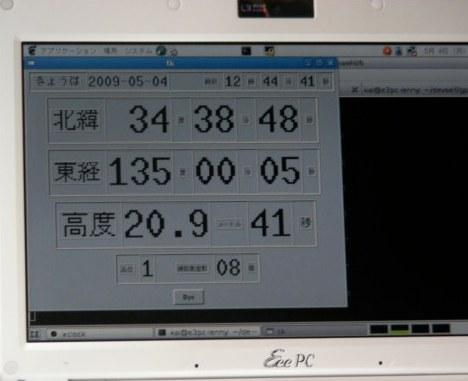
\includegraphics[scale=0.6]{image200912/handmadegpsloger1.jpg}
\end{figure*}
\item $B8=:_0LCVCO?^I=<(Nc(B
\begin{figure*}[h!]
    \centering
    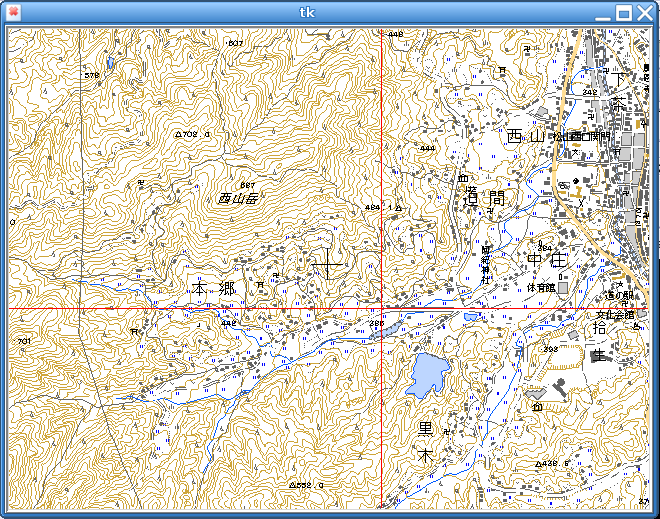
\includegraphics[scale=0.6]{image200912/handmadegpsloger2.png}
\end{figure*}
\clearpage
\item $B%W%m%0%i%`Nc#1!'%G!<%?$N%m%0(B
\begin{commandline}
#!	/usr/bin/python2.5
# -*- coding: utf8 -*-

#********************************************
#	
#	Created			.... 2010-01-03
#	updated			.... 2010-07-11
#	
#	object:			logging data from gps  reeiver	
#	
#	input device:	gps receiver (N103)
#	output-1:		file
#	output-2:		terminal
#	
#	data format:	NMEA-0183.
#	
# ********************************************

import	serial

# open read/write file.
d_fname = "logdata01"
fw = open(d_fname, 'w')
fw.close()
fw = open(d_fname, 'a')

# open serial line.
ser = serial.Serial('/dev/ttyUSB0', 38400, timeout = 3)
serstr = ser.portstr + "\n"
print ser.portstr

for  i in range(10):
	line = (ser.readline() ).strip() 	# get 1 line 'GPGGA' sentence.
	print line
	line += "\n"
	fw.write(line)						# write new data to log file.

fw.close()
ser.close()
\end{commandline}
%\clearpage
\item $B%W%m%0%i%`Nc#1!'%G!<%?$N%m%0(B
$B%W%m%0%i%`Nc#2!'!!8=:_0LCV!J0^EY!K$NI=<((B
\begin{commandline}
#!	/usr/bin/python2.5
# -*- coding: utf8 -*-

#********************************************
#	
#	Created			.... 2009-02-07 ...
#	updated			.... 2010-07-11
#	
#	object:			display latitude on the screen	
#	
#	input device:	gps receiver (N103)
#	output-1:		file
#	output-2:		screen
#	
#	data format:	NMEA-0183.
#	
#********************************************

import	serial
import Tkinter as Tk
import	string
# import os.path


root = Tk.Tk()

buff_dLa = Tk.StringVar()
buff_mLa = Tk.StringVar()
buff_sLa = Tk.StringVar()
buff_dLa.set('')
buff_mLa.set('')
buff_sLa.set('')

# define function
def cmd_quit():
	root.destroy()

# display frame

# define display font
dfont = 'Monospace '
dfont12 = dfont + '12'
dfont18 = dfont + '18'
dfont24 = dfont + '24'
dfont28 = dfont + '28'
dfont48 = dfont + '48'

# display latitude
f1 = Tk.Frame(master=None, relief= 'ridge', bd=3)
b10 = Tk.Label(f1, text="$BKL0^(B", font=dfont24, relief = 'ridge')
b11 = Tk.Label(f1, textvariable = buff_dLa, font=dfont48, relief = 'ridge')
b12 = Tk.Label(f1, text="$BEY(B", relief = 'ridge')
b13 = Tk.Label(f1, textvariable = buff_mLa, font=dfont48, relief = 'ridge')
b14 = Tk.Label(f1, text="$BJ,(B", relief = 'ridge')
b15 = Tk.Label(f1, textvariable = buff_sLa, font=dfont48, relief = 'ridge')
b16 = Tk.Label(f1, text="$BIC(B", relief = 'ridge')

for e in [b10, b11, b12, b13, b14, b15, b16 ]:
	e.pack(side='left', padx=5)

# display Exit Button
b99 = Tk.Button(master=None, text="Bye", command=cmd_quit)

# display Tate ni naraberu.
for e in [ f1, b99]:
# for e in [ f0, f1, f2, f3, f4, b99]:
	e.pack(side='top', padx=5, pady=5)

def showtime():
	# get 'GPGGA' sentence from gps receiver.
	ser = serial.Serial('/dev/ttyUSB0', 38400, timeout = 3)
	# ser = serial.Serial('/dev/ttyUSB0', 4800, timeout = 3)
	print ser.portstr
	line = ser.readline()
	words = line.split(',')
	while( not words[0] == '$GPGGA'):
		line = ser.readline()
		words = line.split(',')
	print line
	ser.close()

	# latitude
	lati = words[2]
	deg_lati = " " + lati[:2]
	min_lati = lati[2:4]
	sec_lati = str( int(float(lati[4:]) * 60 ) ).zfill(2)
	gpslati = 'latitude = ' + deg_lati + ':' + min_lati + ':' + sec_lati + ' ' + words[3] + '  '

	buff_dLa.set(deg_lati)
	buff_mLa.set(min_lati)
	buff_sLa.set(sec_lati)

	root.after(1, showtime)

showtime()
root.mainloop()
\end{commandline}
\end{enumerate}

% from debianmeetingresume201004-kansai.tex
\dancersection{$B%O%C%+!<$K0lJb6a$E$/(B Tips $B!A@55,I=8=JT!A(B}{$B;32<9/@.!w5~ETI\8~F|;T(B}
\index{$B$;$$$-$R$g$&$2$s(B@$B@55,I=8=(B}
\index{sed}
\index{grep}

\subsection{$B@55,I=8=$H$O(B}

$B8!:w$dCV49$J$I%F%-%9%H=hM}$G;HMQ$9$k8zN(E*$J%Q%?!<%s%^%C%A%s%0$NI=8=J}K!(B
$B$G$9!#(B
$B%U%!%$%kL>$K;H$&(B *, ? $B$H35G0$OF1$8$G$9!#(B 
$B:#2s!"@bL@$9$k$N$O(B

\begin{commandline}
^$.[]*\(){}    
\end{commandline}
$B$N$?$C$?(B11$BJ8;z!\?t;z$G$9!#(B

\subsection{$B;vA02]Bj(B}

/etc/passwd $B$r2r@O$7$F%f!<%6(B bin$B$N%m%0%$%s%7%'%k$rI=<($7$J$5$$(B
\begin{enumerate}
\item $B;W9M$K6a$$2rEzNc(B
\begin{commandline}
% grep '^bin:' /etc/passwd|cut -d: -f7  
\end{commandline}
\item $B6u5$$rFI$s$G@55,I=8=$r;H$C$?2rEz(B
\begin{commandline}
% sed -n -e 's/^bin:.*:\([^:]*\)$/\1/p' /etc/passwd        
\end{commandline}
\end{enumerate}

\subsection{$B@55,I=8=$G;H$&J8;z(B}
\subsubsection{ \^ ~$B$H(B \$}
\begin{description}
      \item[{\tt \^}] $B9TF,$K0lCW(B
      \item[{\tt \$}] $B9TKv$K0lCW(B
\end{description}
$B9TF,(B(\^\ ), $B9TKv(B(\$ )$B$K%^%C%A$5$;$k>l9g$NNc(B:
\begin{commandline}
% grep '^bin:' /etc/passwd
% grep '/bash$' /etc/passwd 
\end{commandline}
grep $B0J30$G$b!"(Bemacs $B$d(B vi $B$G$bF1$8MM$K;H$($k!#$b$A$m$s(B, perl $B$d(B awk $B$G$b(B...
\begin{commandline}
emacs   ->  RE search: ^bin
vi      ->  /bash$
\end{commandline}

\subsubsection{{\tt .} $B%T%j%*%I(B}

$B2?$+0lJ8;z$K0lCW$9$k!#(B
$BJ8;z?t$@$1$,0lCW$9$l$PNI$$$H$-$d(B
$B2?$+J8;z$,$"$k$3$H$,=EMW$J$H$-$K;H$&!#(B

\subsubsection{$BNs5s(B}

$BNs5s$7$?$I$l$+$K0lCW$5$;$?$$$H$-!#(B
$BNc(B: bin $B$d(B root $B$J$I(B b, r $B$G;O$^$k%f!<%6$rI=<((B
\begin{commandline}
% grep '^[br]' /etc/passwd
\end{commandline}
$B$[$+$K$O(B
\begin{commandline}
[! " \# ] $B!!(B!, ", \# $B$K0lCW(B
[0-9] $B!!H>3Q?t;z#1J8;z$K0lCW(B
[A-Za-z] $B!!1Q;z$K0lCW(B
\end{commandline}

\subsubsection{[\^~$BNs5s(B]}

$BNs5s$7$?$I$l$K$b0lCW$5$;$?$/$J$$$H$-!#(B
$BNc(B: daemon $B$d(B sys $B$J$I(B b, r $B0J30$G;O$^$k%f!<%6$rI=<((B 
\begin{commandline}
% grep '^[^br] /etc/passwd    
\end{commandline}
$B"(9TF,$rI=$9(B \^~ $B$H(B [~] $BFb$N(B \^~ $B$H$O!"F1$8J8;z$@$,0UL#$,0c$&(B

\subsection{*$B!J%"%9%?%j%9%/!K(B}

$B$9$0A0$NJ8;z!?@55,I=8=(B0$B2s0J>e$K0lCW!#(B
$BNc(B:
\begin{commandline}
$B2?$,$$$/$D$"$C$F$b0lCW(B
  .* 
$B%[%o%$%H%9%Z!<%9$,$$$/$D$"$C$F$b0lCW(B
  [<space><tab>]* 
\end{commandline}

\subsubsection{\{n,m\}}

$B$9$0A0$NJ8;z!?@55,I=8=(Bn$B2s0J>e(Bm $B2s0J2<$K0lCW!#(Bm $B$O>JN,2DG=(B
\begin{commandline}
$B%[%o%$%H%9%Z!<%9$,(B1$B8D0J>e$"$l$P0lCW(B
[<space><tab>]\{1,\} 
$B?t;z$,(B1$BJ8;z0J>e#5J8;z0J2<!JNc$($P$6$C$H(B short $B$NHO0O!K$"$l$P0lCW(B
[0-9]\{1,5\} 
\end{commandline}

\subsubsection{( ) $B$H(B $\backslash$n (n=1..9)}

($B!!(B) $B$G0O$s$@$H$3$m$r=g$K(B $\backslash$1 ,$\backslash$2 ... $B$H$7$F;H$($k!#(B
$BCV49$K;H$&$HCV4985$N0lIt$r;H$($k!#(B
vi $B$N(B ex $B%b!<%I$d!"(Bemacs $B$N(B replace regexp $B$G$b;H$($k!#(B 
$BNc(B:
\begin{commandline}
# aaa bbb $BEy!"9TF,$KF1$8J8;z$,#3$D$"$k;~$K0lCW(B 
% echo 'aaa' | grep '^\(.\)\1\1'
# abab 1212 $BEy!"9TF,$+$i#2J8;z$N7+$jJV$7$K0lCW(B 
% echo 'abab' | grep '^\(.\)\(.\)\1\2'
% echo 'abcd' | sed - e 's/^\(.\)\(.\).*$/1$BJ8;zL\$O(B \1$B!"(B2$BJ8;zL\$O(B \2 $B$G$9(B/' 
\end{commandline}

\subsection{$B;vA02]Bj$N6u5$$rFI$s$@2rEz$r%l%S%e!<(B}
\begin{commandline}
sed -n -e 's/^bin:.*:\([^:]*\)$/\1/p' /etc/passwd
\end{commandline}
$B$3$l$O!"(B

 \begin{quote}
 \begin{verbatim}
$B!P(B
$B9TF,$,(Bbin:$B!!$G(B
$B2?$+J8;z$,#0J8;z0J>e$"$C$F(B
: $B$,$"$C$F(B
: $B0J30$,#00J>e$"$k$H$3$m$r(B1$BHVL\$N%P%C%U%!$K$$$l$F(B
$B9TKv(B
$B!Q(B
 \end{verbatim}
 \end{quote}


$B$H$$$&%Q%?!<%s$,$"$l$P!"(B1$BHVL\$N%P%C%U%!$rI=<($9$k!#(B

\subsection{$B<BNc(B}
\subsubsection{ssh $B%"%?%C%+!<$r%V%m%C%/$9$k(B}
/var/log/daemon.log $B$K(B
\begin{commandline}
Apr 11 04:46:07 ns sshd[31776]: Invalid user oracle from 211.233.73.66
Apr 11 09:17:05 ns sshd[5607]: Did not receive identification string from 211.155.227.20
\end{commandline}
$B$N$h$&$J9T$,$"$l$P!"$=$N(B IP $B%"%I%l%9$r(B /etc/hosts.deny $B$KEPO?$9$k!#(B
\begin{commandline}          
#! /bin/sh
# Apr 11 04:46:07 ns sshd[31776]: Invalid user oracle from 211.233.73.66
# Apr 11 09:17:05 ns sshd[5607]: Did not receive identification string from 211.155.227.20

export LANG=C
HOSTSDENY=/etc/hosts.deny

sed -n \
        -e 's/^.* sshd.*: Invalid user \(.*\) from \([0-9][0-9\.]*\)/\1 \2/p' \
        -e 's/^.* sshd.*: Did not receive identification string from \([0-9][0-9\.]*\)/\1/p' \
        /var/log/daemon.log | sort -u |
while read NAME IP 
do
        # /etc/hosts.deny
        L=`grep '^ALL : '$IP'$' $HOSTSDENY`
        if [ "$L" = "" ]
        then
                echo "ALL : $IP" >> $HOSTSDENY
        fi
done
\end{commandline}


\subsubsection{%
$B%m!<%I%"%Y%l!<%8$,#30J>e$J$i!"F|;~$H(Bps ax $B$N7k2L$r(B /tmp/highload $B$K;D$9(B}

\begin{commandline}
# LANG=C uptime
11:57PM  up 165 days,  2:26,  1 user,  load average: 0.00, 0.06, 0.07
\end{commandline}
$B>e5-$N%m!<%I%"%Y%l!<%8$N0l$DL\$r@Z$j=P$9(B
\begin{commandline}
#! /bin/sh 
LOAD=`LANG=C /usr/bin/uptime | sed -e 's/^.*: \([0-9]*\)\.[0-9]*,.*$/\1/'
if [ "$LOAD" -ge 3 ]
then
      echo >> /tmp/highload
      date >> /tmp/highload
      ps ax >> /tmp/highload
fi
\end{commandline}

\subsubsection{$B%-%b(B}

$B9TF,$b$7$/$O9TKv$r5/E@$K%Q%?!<%s%^%C%A$r$9$k$HNI$$>l9g$,B?$$!#(B
\begin{quote}
$B"*(B \^\ $B$H(B \$\ $B$H$r3hMQ(B
\end{quote}
$B%9%Z!<%96h@Z$j$O(B TAB $B$H%9%Z!<%9$,$$$/$D$"$k$+$o$+$i$J$$!#(B
\begin{quote}
$B"*(B * $B$d(B \{n,m\} $B$r3hMQ(B
\end{quote}
\begin{commandline}
[<SP.><TAB>][<SP><TAB>]*
[<SP.><TAB>]\{1,\}
\end{commandline}

\subsection{$B$*$o$j$K(B}

$B@55,I=8=$r$&$^$/;H$$$3$J$;$l$PA`:n$,>/$J$/$J$j!"(B
$B$b$7$/$O%9%/%j%W%H$,>.$5$/$G$-$F8zN(E*!#(B $B@55,I=8=$r%^%9%?$7$F!"%O%C%+!<$K0lJb6a$E$3$&(B!

%-------------------------------------------------------------------------------
% from debianmeetingresume201003.tex
\dancersection{$B%K%e!<%i%k%M%C%H%o!<%/$G2hA|G'<1$7$F$_$?(B}{$BK\>190E5(B}
%-------------------------------------------------------------------------------
\index{neural network}
\index{back propagation}
\index{$B$,$>$&$K$s$7$-(B@$B2hA|G'<1(B}

\subsection{$B$O$8$a$K(B}

$B%I%-%e%a%s%H%9%-%c%J$GK\$r%9%-%c%s$7$?:]!"2hA|$N%5%$%:$,Bg$-$9$.(B
$B$k$?$aJ]B8$KE,$7$^$;$s!#$3$N2hA|$r#2CM2hA|$H%0%l!<%9%1!<%k!"%+%i!<(B
$B2hA|$=$l$>$l$N=hM}$r2C$($k$3$H$G%U%!%$%k%5%$%:$r=L>.$7!"%K%e!<%i(B
$B%k%M%C%H$rMQ$$$k$3$H$K$h$j$"$kDxEY<+F02=$G$-$J$$$+$H9M$($^$7$?!#(B
$B:#2s$O%K%e!<%i%k%M%C%H$H$7$F0lHLE*$J;0AX%Q!<%;%W%H%m%s$rMQ$$$?2h(B
$BA|H=JL$N0lNc$r2r@b$7$^$9!#(B

\subsection{$B;0AX%Q!<%;%W%H%m%s$H%P%C%/%W%m%Q%2!<%7%g%s(B}

\subsubsection{$B;0AX%Q!<%;%W%H%m%s(B}

$B;0AX%Q!<%;%W%H%m%s$OF~NOAX!"Cf4VAX!"=PNOAX$HJL$l$?;0AX$N3F%K%e!<(B
$B%m%s$,=E$_$H8F$P$l$k78?t$G7k$P$l$?%b%G%k$H$J$j$^$9(B(\fgref{fig:neuralnet01})$B!#(B

\begin{figure}[H]
\begin{center}
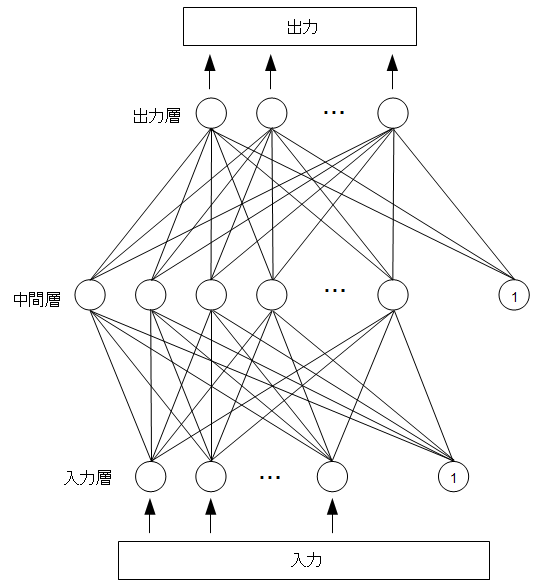
\includegraphics[width=0.45\hsize]{image201003/neuralnet01.png}
\caption{$B;0AX%Q!<%;%W%H%m%s(B}
\label{fig:neuralnet01}
\end{center}
\end{figure}

$B$=$l$>$l$N=E$_$O<B?t$GI=$5$l!"%Q!<%;%W%H%m%s$,5!G=$9$k$?$a$K$O$3(B
$B$N=E$_$,E,@Z$K@_Dj$5$l$F$$$kI,MW$,$"$j$^$9!#$"$kF~NO$,M?$($i$l$?(B
$B:]!"F~NOCM$K=E$_$r3]$19g$o$;!"$=$l$>$l$N9g7W$K<!$N$h$&$J%7%0%b%$(B
$B%I4X?t$rE,MQ$7$??tCM$rCf4VAX$N;}$DCM$H$7$^$9!#(B

\begin{multicols}{2}

\begin{figure}[H]
\begin{center}

\begin{equation*}
 \varsigma_1(x) = \frac{1}{1+e^{-x}}
\end{equation*}
\end{center}
\caption{$B%7%0%b%$%I4X?t$N<0(B}
\end{figure}

\begin{figure}[H]
\begin{center}
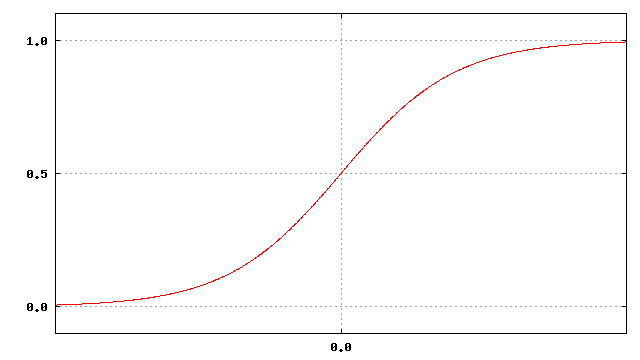
\includegraphics[width=1.0\hsize]{image201003/neuralnet03.png}
\caption{$B%7%0%b%$%I4X?t$N%0%i%U(B}
\end{center}
\end{figure}

\end{multicols}

$B3F=PNOAX$bF1MM$N7W;;$,$J$5$l!"%Q!<%;%W%H%m%s$N=PNO$,9T$o$l$^$9!#(B

\subsubsection{$B%P%C%/%W%m%Q%2!<%7%g%s(B}

$BB?AX%Q!<%;%W%H%m%s$GE,@Z$J=PNO$r9T$&$?$a$N3X=,J}K!$H$7$F0lHLE*$J(B
$B$b$N$K%P%C%/%W%m%Q%2!<%7%g%s$,$"$j$^$9!#%P%C%/%W%m%Q%2!<%7%g%s$G(B
$B$O$^$:F~NO$KBP$9$k@5$7$$=PNO(B($B65;U?.9f(B)$B$rB??tMQ0U$7!"3F=E$_$r%i%s(B
$B%@%`$K@_Dj$7$^$9!#MQ0U$5$l$?F~NO$KBP$7$F%i%s%@%`$J=E$_$+$i%Q!<%;(B
$B%W%H%m%s$N=PNO$O$G$?$i$a$JCM$H$J$j$^$9$,!"$3$N=PNO$H65;U?.9f$H$N(B
$BHf3S$+$i=PNOAX$HCf4VAX$N4V$N=E$_$r=$@5$7!"<!$$$GCf4VAX$HF~NOAX$N(B
$B=E$_$r=$@5$9$k$3$H$GE,@Z$J=E$_$rC5$7=P$7$^$9!#(B

\subsection{$BB-$7;;$H0z$-;;$r3X=,$7$F$_$k(B}

$B:n@.$7$?%Q!<%;%W%H%m%s$H%P%C%/%W%m%Q%2!<%7%g%s$,@5>o$KF0:n$9$k$+(B
$B$r3N$+$a$^$9!#<!$N$h$&$JF~NO$rMQ0U$7$^$7$?!#(B

\begin{commandline}
# $B3X=,MQ65;U?.9f%Z%"(B
0.40,0.20	0.60,0.20
0.30,0.20	0.50,0.10
0.80,0.10	0.90,0.70
0.20,0.10	0.30,0.10
0.50,0.50	1.00,0.00
0.60,0.20	0.80,0.40
# $BI>2AMQF~NOCM(B
*0.50,0.10
*0.50,0.40
*0.10,0.40
\end{commandline}

$BF~NOCM$H65;U?.9f$N%Z%"$O%?%V6h@Z$j$N:8$,F~NO!"(B
$B1&$,F~NO$KBP$9$k65;U?.9f$G$9!#(B
$B$3$3$G$OB-$7;;$H0z$-;;$N65;U?.9f$rM?$($^$7$?!#(B

\newpage

$B<B9T$7$^$9!#(B

\begin{commandline}
$ ./backprop.exe sample.txt 10000
       0 0.87640153
     100 0.26410368
     200 0.10289131
     300 0.03820243
     400 0.02475167

...($BCfN,(B)...

    9600 0.00077714
    9700 0.00077174
    9800 0.00076646
    9900 0.00076128
0.4000, 0.2000  0.60, 0.18      0.60, 0.20
0.3000, 0.2000  0.50, 0.11      0.50, 0.10
0.8000, 0.1000  0.90, 0.70      0.90, 0.70
0.2000, 0.1000  0.30, 0.11      0.30, 0.10
0.5000, 0.5000  0.98, 0.02      1.00, 0.00
0.6000, 0.2000  0.80, 0.41      0.80, 0.40
0.5000, 0.1000  0.63, 0.35
0.5000, 0.4000  0.93, 0.06
0.1000, 0.4000  0.87, 0.00
Ratio=0.00075626
Count=10000
Sample=6
Input=2
Middle=4
Output=2
InputHidden0=-2.57936471,-2.20525001,-1.50656422,4.05055823,-0.66468037
InputHidden1=-1.29032439,8.71632107,-1.24344376,-0.85214732,-0.66468037
InputHidden2=2.04901840,-2.94096519,1.04866634,-1.98825291,0.29698485
HiddenOutput0=-2.91458436,-1.16992032
HiddenOutput1=5.84673832,-6.31188860
HiddenOutput2=-1.80018561,-0.42470539
HiddenOutput3=3.60356071,3.84028669
HiddenOutput4=1.40998866,-1.22885398
\end{commandline}

$BMj$j$J$$$J$,$i$b$=$l$J$j$N1i;;7k2L$,=PNO$5$l$F$$$^$9!#I>2A$H$7$F(B
$B:G8e$N?tCM$O8:;;7k2L$,Ii$K$J$k$O$:$J$N$G$9$,!"%7%0%b%$%I4X?t$rDL(B
$B$9$3$H$G=PNO$,(B0.0$B!A(B1.0$B$H$J$k$?$a@5>o$J7k2L$,F@$i$l$^$;$s!#(B

\subsection{$B2hA|$rJ,N`$9$k$?$a$NF~NOCM$r9M$($k(B}

$B2hA|H=JL$NF~NOCM$H$7$F<!$NCM$r;HMQ$7$^$7$?!#(B

\begin{itemize}
\item $BJd@5$7$?2hA|$N(BRGB$B$N:9(B
\item $BHyJ,$7$?2hA|$N(BRGB$B$N:9(B
\item $B2hA|$NJ#;($5!#(B
\item $B;H$o$l$F$$$k?'$N?t(B
\item $BJ?6Q:LEY(B
\item FFT$B=hM}$7$?2hA|$NL@$k$$%T%/%;%k$rMxMQ$9$k(B
\item HSV$B$KJQ49$7!"?'AG$NJ?6Q$rMxMQ$9$k(B
\item $B?'AG$NJ,;6$rMxMQ$9$k(B
\end{itemize}

$B$3$NCf$+$iJ8>O$H3($NH=JL$H$7$F2hA|$N(BFFT$B$r!"%+%i!<2hA|$NH=JL$H$7(B
$B$F(BHSV$B$X$NJQ49$r2r@b$7$^$9!#(B

\subsubsection{$B%b%N%/%m2hA|$N=hM}!&J8;z$H3($rJ,N`$7$F$_$k(B}

$B=D=q$-$NJ8>O$O2#J}8~$K0lDj$N<~GH?t$r;}$C$F$$$k$H8+$J$9$3$H$,=PMh(B
$B$^$9!#$3$l$K$h$j!"J8>O$N2hA|$rHyJ,$7(BFFT$B=hM}$r9T$C$?7k2L$+$i?6I}(B
$B$rIA2h$9$k$H$G!"L@$k$/8w$kE@$,8=$l$k$3$H$,$o$+$j$^$7$?!#(B

\begin{figure}[H]
\begin{center}
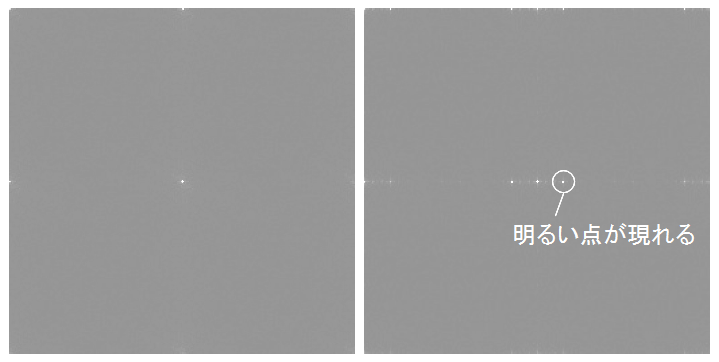
\includegraphics[width=0.9\hsize]{image201003/neuralnet04.png}
\caption{$B%$%i%9%H$HJ8>O$rHyJ,$7$?2hA|$N(BFFT$B7k2L(B}
\end{center}
\end{figure}

$B$3$NE@$NL@$k$5$rF~NOCM$H$9$k$3$H$G!"J8>O$H%$%i%9%H$NH=JL$,9T$($k(B
$B$H4|BT$G$-$^$9!#(B

\subsubsection{$B%+%i!<2hA|$H$=$&$G$J$$2hA|$rJ,N`$7$F$_$k(B}

$B%+%i!<2hA|$H%b%N%/%m2hA|$O2hA|$N(BRGB$B$r(BHSV$B$KJQ49$7!"?'Aj$+$iH=JL$r(B
$B9T$C$F$$$^$9!#(B

RGB$B$N$&$A$+$i:GBg$N$b$N$r(BMAX$B!":G>.$N$b$N$r(BMIN$B$H$9$k$H?'Aj$O(B\fgref{fig:cal-hue}$B$N(B
$B<0$H$J$j$^$9!#(B

\begin{figure}[H]
\begin{center}
\begin{align*}
 H = & 60 \frac{G-B}{MAX-MIN} + 0, & if MAX = R\\
     & 60 \frac{B-R}{MAX-MIN} + 120,   & if MAX = G\\
     & 60 \frac{R-G}{MAX-MIN} + 240,   & if MAX = B\\
\end{align*}
\caption{$B?'Aj$N7W;;<0(B}
\label{fig:cal-hue}
\end{center}
\end{figure}

$B%b%N%/%m2hA|$O?'Aj$r;}$?$J$$$?$a!"(BRGB$B$N$&$A@D$N@.J,$r8:$i$9$3$H(B
$B$G2+?'$$%U%#%k%?$r$+$1$^$7$?!#$3$&$9$k$3$H$G%b%N%/%m2hA|$N?'Aj$N(B
$BJ?6Q$O2+?'$H$J$j!"%+%i!<$H%b%N%/%m$rH=JL$9$k$?$a$NF~NOCM$H$7$F4|(B
$BBT$G$-$^$9!#(B

\subsection{$B3X=,$N>r7o(B}

$B%K%e!<%i%k%M%C%H$N3X=,$O<!$N>r7o$G9T$$$^$7$?!#(B

\begin{itemize}
\item $BF~NOAX(B8$B8D(B
\item $BCf4VAX(B24$B8D(B
\item $B=PNOAX(B2$B8D(B
\item $B%5%s%W%k$H$7$F;HMQ$7$?K\(B23$B:}(B($BL!2h(B2$B:}(B/$BJ88K(B20$B:}(B/$B5;=Q=q(B1$B:}(B)
\item $B%Z!<%8?t(B6742$B%Z!<%8(B
\item $B3X=,2s?t(B50$BK|2s(B
\end{itemize}

$B<B:]$K$3$N>r7o$G3X=,$r9T$C$?:]!"(B
Core i7 950$B$G(B7$B;~4V<e$N3X=,;~4V$H$J$j$^$7$?!#(B

\subsection{$BH=JL$N@:EY(B}

$B:n@.$5$l$?%D!<%k$G<B:]$KH=JL$r9T$$!"$=$N@:EY$rD4$Y$^$7$?!#I>2A$K(B
$B;HMQ$7$?K\$O3X=,$K;H$o$l$F$$$J$$$b$N$rA*$S$^$7$?!#(B

\begin{description}
 \item[$B%5%s%W%k(B1. $B%i%$%H%N%Y%k:G?74,(B] \mbox{}\\
    240$B%Z!<%8Cf!"?M4V$NH=JL$H?)$$0c$&%Z!<%8$,(B2$B%Z!<%8!#FbLu$O%+%i!<(B
    12$B%Z!<%8!"%0%l!<%9%1!<%k(B15$B%Z!<%8!"J8>O(B213$B%Z!<%8!#$=$N$&$A%$(B
    $B%i%9%H$,J8>O$HH=JL$5$l$?$N$,(B1$B%Z!<%8!"J8>O$,%$%i%9%H$HH=JL$5(B
    $B$l$?$N$,(B1$B%Z!<%8!#(B
 \item[$B%5%s%W%k(B2. SF$BD9JT%7%j!<%:$N>e4,(B] \mbox{}\\
    568$B%Z!<%8Cf!"?M4V$NH=JL$H?)$$0c$&%Z!<%8$O$J$7!#FbLu$O%+%i!<(B5
    $B%Z!<%8!"%0%l!<%9%1!<%k(B3$B%Z!<%8!"J8>O(B560$B%Z!<%8!#(B
 \item[$B%5%s%W%k(B3. $B%m!<%^?M$N%7%j!<%:(B1$B4,(B] \mbox{}\\
    216$B%Z!<%8Cf!"?M4V$NH=JL$H?)$$0c$&%Z!<%8$O(B5$B%Z!<%8!#FbLu$O%+%i!<(B
    6$B%Z!<%8!"%0%l!<%9%1!<%k(B9$B%Z!<%8!"J8>O(B201$B%Z!<%8!#$=$N$&$A%+%i!<(B
    4$B%Z!<%8$NH=JL$K<:GT$7$F$$$^$9$,!"860x$O%+%P!<%Z!<%8$,%Y!<%8%e(B
    $B$GJ8>O$H$7$FH=JL$5$l$^$7$?!#CO?^$d%$%i%9%H$HJ8>O$,:.$8$C$?%Z!<(B
    $B%8$b3X=,DL$jJ8>O$H$7$FH=JL$5$l$F$$$^$9!#(B
 \item[$B%5%s%W%k(B4. 50$BG/A0$KH/9T$5$l$?3)@n>^<u>^:n(B] \mbox{}\\
    40$BG/6a$/A0$K=PHG$5$l$?K\$G!"(B280$B%Z!<%8Cf!"?M4V$NH=JL$H?)$$0c(B
    $B$&%Z!<%8$,(B16$B%Z!<%8!#FbLu$O%+%i!<(B6$B%Z!<%8!"J8>O(B274$B%Z!<%8!#H=JL(B
    $B$N<:GT$,B?$$M}M3$OJQ?'$H?dB,$5$l!"%+%i!<$@$1$G$O$J$/%$%i%9%H(B
    $B$H$bB?$/4V0c$C$FH=JL$5$l$^$7$?!#(B
\end{description}

%-------------------------------------------------------------------------------
% from debianmeetingresume201003.tex
\dancersection{Weka$B$r;H$C$F$_$k(B}{$B$^$($@$3$&$X$$(B}
%-------------------------------------------------------------------------------
\index{Weka}
\subsection{$B35MW(B}

$B%K%e!<%i%k%M%C%H%o!<%/$r$O$8$a$H$9$k%G!<%?%^%$%K%s%0$r0lHL?M$,;H$&$K$O!"(B
$BA0>O$NK\>1$5$s$N%M%?$N$h$&$KM}O@$rM}2r$7$?>e$G<+J,$G%W%m%0%i%`$r:n$i$J$$$H$$$1(B
$B$J$$$H$9$k$H!"Hs>o$K%O!<%I%k$,9b$$$H;W$$$^$9!#3X@8$N$3$m$K3X$s$@$j!"8&5f(B
$B$7$F$$$?$+!";E;v$H$7$FIaCJ$+$i07$C$F$$$k$h$&$J?M$G$J$1$l$P!"C18l$H$7$F$O(B
$B<*$K$7$?$3$H$,$"$C$F$b!"$J$s$@$+$h$&J,$+$i$s!"$H$$$&?M$,$[$H$s$I$G$O$J$$(B
$B$G$7$g$&$+!#(B\footnote{Debian $BJY6/2q$N>oO"$O$`$7$mCN$C$F$$$k?M$NJ}$,B?$$(B
$B$N$+$b$7$l$^$;$s$,!">/$J$/$H$b;d$OC18l$r<*$K$7$?$3$H$,$"$k%l%Y%k$G$9!#(B}
\index{$B$G!<$?$^$$$K$s$0(B@$B%G!<%?%^%$%K%s%0(B}

$B$=$3$G!"%P%C%/%0%i%&%s%I$H$7$F%K%e!<%i%k%M%C%H%o!<%/$@$1$G$J$/!"%G!<%?%^(B
$B%$%K%s%0$N4pACCN<1$r;}$C$F$$$J$$;d$HF1$8$h$&$JN)>l$N?M$G$b!"(BDebian $B$J$i(B
$B5$7Z$K;n$7$F$_$k4D6-$r@0$($F!"<h$j9g$($:;H$C$F$_$k$3$H$,$G$-$k$h!"$H$$$&(B
$B<q;]$G!"(BWeka $B$H$$$&%D!<%k$r>R2p$7$^$9!#(B

\subsection{Weka$B$H$O(B}

Weka $B$H$O!"(B``Waikato Environment for Knowledge Analysis''$B$NN,$G!"%K%e!<(B
$B%8!<%i%s%I$N9qN)%o%$%+%HBg3X(B\footnote{\url{http://www.waikato.ac.nz/}}$B$G(B
GPL $B$N$b$H%*!<%W%s%=!<%9$G3+H/$5$l$F$$$k%G!<%?%^%$%K%s%0%D!<%k$G$9!#(B
\footnote{\url{http://www.cs.waikato.ac.nz/~ml/weka/index.html}} Java $B$G(B
$B=q$+$l$F$$$^$9!#(B

\subsection{$B%$%s%9%H!<%k(B}

Debian $B$G$O%Q%C%1!<%8$,MQ0U$5$l$F$$$^$9!#(B

\begin{commandline}
$ sudo apt-get install weka
\end{commandline}

\subsection{Weka$B$N;H$$J}(B}

$B%3%^%s%I%i%$%s$G(B \texttt{weka} $B%9%/%j%W%H$r<B9T$7$^$9!#(B

\begin{commandline}
$ weka &
\end{commandline}

$B$9$k$H(B Weka $B$N%&%#%s%I%&$,5/F0$7$^$9!#(B
$B$=$3$+$i!"(B``Applications'' $B$N(B ``Explorer''$B$r<B9T$9$k$H!"(B
Weka Explorer $B$,5/F0$7$^$9!#(B

\begin{figure}[H]
\begin{minipage}{0.4\hsize}
 \begin{center}
 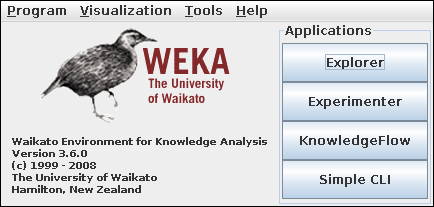
\includegraphics[width=1\hsize]{image201003/weka0.png}
 \caption{Weka $B5/F0%a%K%e!<(B}
 \end{center}
\end{minipage}
\begin{minipage}{0.5\hsize}
 \begin{center}
 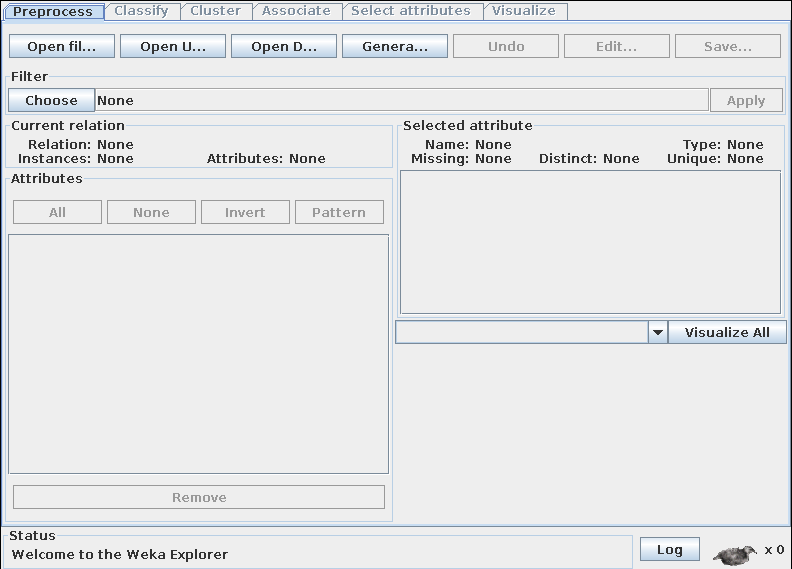
\includegraphics[width=1\hsize]{image201003/weka1.png}
 \caption{Weka Explorer}
 \end{center}
\end{minipage}
\end{figure}

\subsubsection{Weka $B$G07$&%G!<%?%U%)!<%^%C%H(B}

Weka $B$G$O!"(BARFF(Attribute-Relation File Format)$B$H$$$&%U%)!<%^%C%H$N%F%-(B
$B%9%H%U%!%$%k$rF~NO%G!<%?$H$7$F07$$$^$9!#(B
\index{arff}

$B%G!<%?%U%)!<%^%C%H$O<!$N$h$&$K$J$j$^$9!#(B

\begin{commandline}
@relation $BL>A0(B $B"+%G!<%?A4BN$NL>A0$r;XDj(B
@attribute $BB0@-L>(B $BB0@-$N7?!!"+%G!<%?$NB0@-!#(B1$B$DL\$N0z?t$OB0@-L>!"(B2$B$D$a$N0z?t$OB0@-%G!<%?$N7?(B
@attribute $BB0@-L>(B $BB0@-$N7?(B
:
:
@data$B!!"+%G!<%?NN0h$N@k8@(B
$B%G!<%?(B,$B%G!<%?(B,$B!D(B,$B%G!<%?(B $B"+(BCSV $B7A<0$G%G!<%?$r5-=R(B
\end{commandline}

\begin{itemize}
\item @relation $B$O%G!<%?A4BN$NL>A0$r;XDj$7$^$9!#(B
\item @attribute $B$O%G!<%?$NB0@-$rI=$7!"(B1$B$DL\$N0z?t$OB0@-L>!"(B2$B$D$a$N0z?t(B
      $B$OB0@-%G!<%?$N7?$rI=$7$^$9!#(B
\item @attribute $B$N%G!<%?7?$K$O!"(Bnumeric, real, integer, string, date$B7?(B
      $B$r;H$($^$9!#(B
      \begin{itemize}
       \item numeric $B$O(B real $B$+(B integer $B$r;XDj$G$-$^$9!#(B
       \item real $B$O<B?t$r;XDj$G$-$^$9!#(B
       \item integer $B$O@0?t$r;XDj$G$-$^$9!#(B
       \item string $B$OJ8;zNs$r;XDj$G$-$^$9!#(B
       \item date $B7?$OF|;~$G!"%G%U%)%k%H$O(B''yyyy-MM-dd'T'HH:mm:ss''$B$H$$(B
	     $B$&=q<0$G$9!#(B
      \end{itemize}
 \item @data $B%G!<%?NN0h$N@k8@$G$9!#(B
       \begin{itemize}
	\item $B$=$N<!$N9T$+$i(B CSV $B7A<0$G%G!<%?$r5-=R$7$^$9!#(B
	\item @attribute $B9T$G>e$+$i@_Dj$7$?=g$K(B CSV $B$N0l9T$G$N:8$+$i1&$X(B
	      $B$N3F%G!<%?$H$J$j$^$9!#(B
       \end{itemize}
\end{itemize}

$B:rG/$N(B11$B7n$NJY6/2q$G(B GNU R $B$G07$C$?8wG.Hq$N%G!<%?$H!"5$>]D#$,8x3+$7$F$$(B
$B$k5$29!"9_?eNL$J$I$N5$>]%G!<%?(B\footnote{\url{http://www.data.jma.go.jp/obd/stats/etrn/index.php}}$B$r;H$C$F$_$^$9!#(B

$B$^$:!"(BCSV $B$G0J2<$N$h$&$K5-=R$7$?$H$7$^$9!#(B
\begin{commandline}
"$BG/(B","$B7n(B","$B9_?eNL9g7W(B(mm)","$BJ?6QF|J?6Q5$29(B($B!n(B)","$BJ?6QF|:G9b5$29(B($B!n(B)","$BJ?6QF|:GDc5$(B
$B29(B($B!n(B)","$BJ?6QIwB.(B(m/s)","$B:GBgIwB.(B(m/s)","$BF|>H;~4V(B(h)","$BEE5$;HMQNL(B(kWh)","$BEE5$;HMQ(B
$BNL(B(kWh)/$BF|(B","$BNA6b(B($B1_(B)/$BF|(B","$B9g7WNA6b(B","$B%,%9;HMQNL(B(m3)","$B%,%9;HMQNL(B(m3)/$BF|(B","$BNA6b(B(
$B1_(B)/$BF|(B","$B9g7WNA6b(B"
2007,1,50,6,10.8,1.1,1,5,188.9,234,6.88235294117647,161.235294117647,5482,9,0.333333333333333,80.962962962963,2186
2007,2,44,7.3,12.6,1.9,1.3,6,198.1,198,7.07142857142857,168.071428571429,4706,9,0.321428571428571,87.7142857142857,2456
(snip)
\end{commandline}

$B$3$l$O!"(BARFF $B%U%)!<%^%C%H$G$O0J2<$N$h$&$K$J$j$^$9!#(B

\begin{commandline}
@relation $B9_?eNL!&5$29(B($BI\Cf;T(B)$B$HEE5$Be!"%,%9Be$N4X78$K$D$$$F(B

@attribute $BG/(B real
@attribute $B7n(B real
@attribute $B9_?eNL9g7W(B(mm) real
@attribute $BJ?6QF|J?6Q5$29(B($B!n(B) real
@attribute $BJ?6QF|:G9b5$29(B($B!n(B) real
@attribute $BJ?6QF|:GDc5$29(B($B!n(B) real
@attribute $BJ?6QIwB.(B(m/s) real
@attribute $B:GBgIwB.(B(m/s) real
@attribute $BF|>H;~4V(B(h) real
@attribute $BEE5$;HMQNL(B(kWh) real
@attribute $BEE5$;HMQNL(B(kWh)/$BF|(B real
@attribute $BNA6b(B($B1_(B)/$BF|(B real
@attribute $B9g7WNA6b(B real
@attribute $B%,%9;HMQNL(B(m3) real
@attribute $B%,%9;HMQNL(B(m3)/$BF|(B real
@attribute $BNA6b(B($B1_(B)/$BF|(B real
@attribute $B9g7WNA6b(B real

@data
2007,1,50,6,10.8,1.1,1,5,188.9,234,6.88235294117647,161.235294117647,5482,9,0.333333333333333,80.962962962963,2186
2007,2,44,7.3,12.6,1.9,1.3,6,198.1,198,7.07142857142857,168.071428571429,4706,9,0.321428571428571,87.7142857142857,2456
(snip)
\end{commandline}

\subsubsection{ARFF $B$r%m!<%I$9$k(B}

$B@h$[$IMQ0U$7$?(B kohnetsu.arff $B$r%m!<%I$7$F$_$^$7$g$&!#(BPreprocess $B%?%V$N(B
Open File $B%\%?%s$r2!$7$^$9!#%@%$%"%m%0$,I=<($5$l$k$N$G!"(Bkohnetsu.arff $B$r(B
$B;XDj$7$^$9!#(B(\fgref{fig:wekaarffload})

ARFF $B%U%!%$%k$rFI$_9~$`$H(B\fgref{fig:wekaarffread}$B$N$h$&$K$J$j$^$9!#(BUTF-8 $B%(%s%3!<%I$G$"$l$P!"(B
$B$4Mw$N$H$*$jF|K\8l$b@5>o$KFI$_9~$a$^$9(B

\begin{figure}[H]
 \begin{minipage}{0.5\hsize}
  \begin{center}
   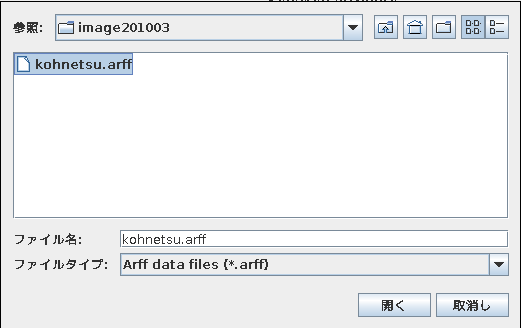
\includegraphics[width=0.9\hsize]{image201003/weka2.png}
   \caption{ARFF $B%U%!%$%k$r%m!<%I$9$k(B}
   \label{fig:wekaarffload}
  \end{center}
 \end{minipage}
 \begin{minipage}{0.5\hsize}
  \begin{center}

   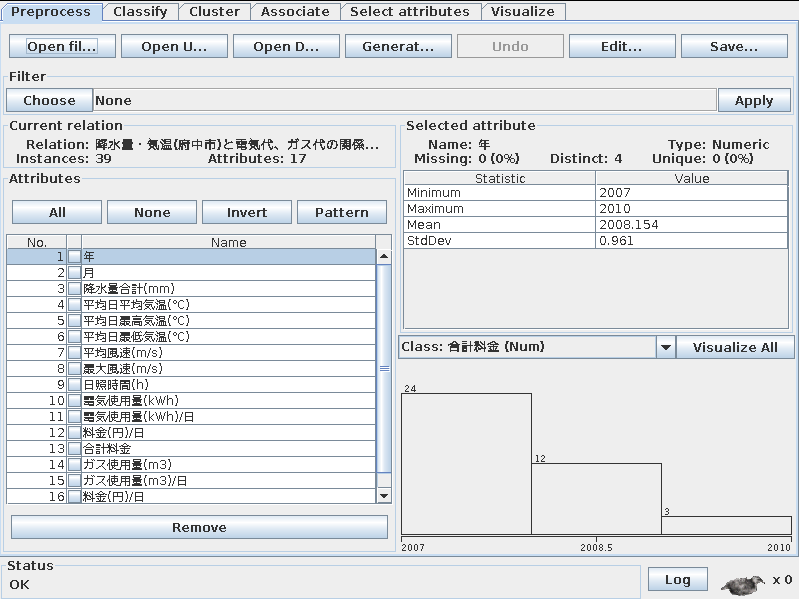
\includegraphics[width=0.9\hsize]{image201003/weka3.png}
   \caption{ARFF $B$+$i%G!<%?$rFI$_9~$s$@7k2L(B}
   \label{fig:wekaarffread}
  \end{center}
 \end{minipage}
\end{figure}

\subsubsection{$B2D;k2=$7$F$_$k(B}

$B$=$l$G$OFI$_9~$s$@%G!<%?$r2D;k2=$7$F$_$^$7$g$&!#(BVisualize $B%?%V$r%/%j%C%/(B
$B$9$k$H(B\fgref{fig:wekavisualize}$B$N$h$&$J%^%H%j%C%/%9$,I=<($5$l$^$9!#(B

$BE,Ev$K3+$$$F$_$^$9!#(BY $B<4$K0lF|$NJ?6Q5$29$N7nJ?6Q(B($B!n(B)$B$H!"(B X $B<4$K0lF|$"$?(B
$B$j$NEE5$;HMQNL(B(kWh)$B$r<h$C$F8+$F$_$k$H(B\fgref{fig:wekavisualizedetail}$B$N$h$&$K$J$j$^$9!#(B

\begin{figure}[H]
 \begin{minipage}{0.5\hsize}
\begin{center}
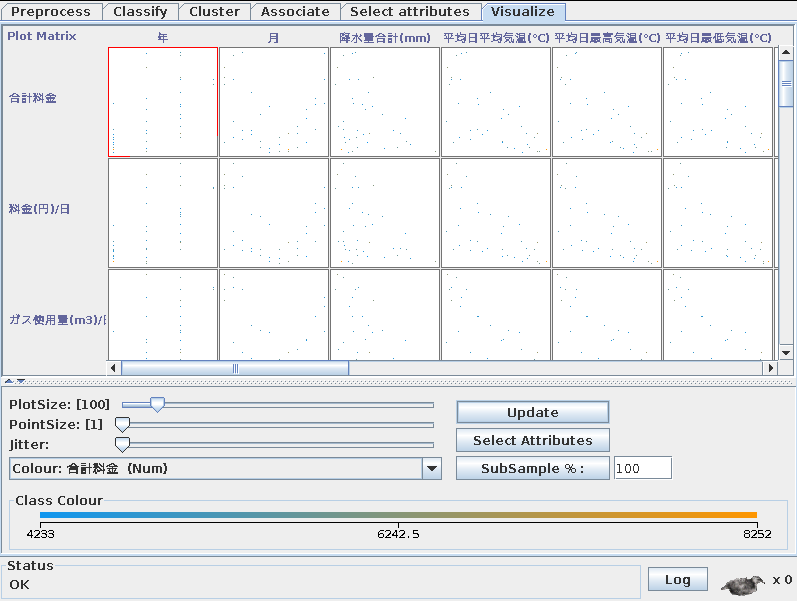
\includegraphics[width=1\hsize]{image201003/weka4.png}
\caption{Visualize $B2hLL(B}
\label{fig:wekavisualize}
\end{center}
\end{minipage}
\begin{minipage}{0.5\hsize}
 \begin{center}
 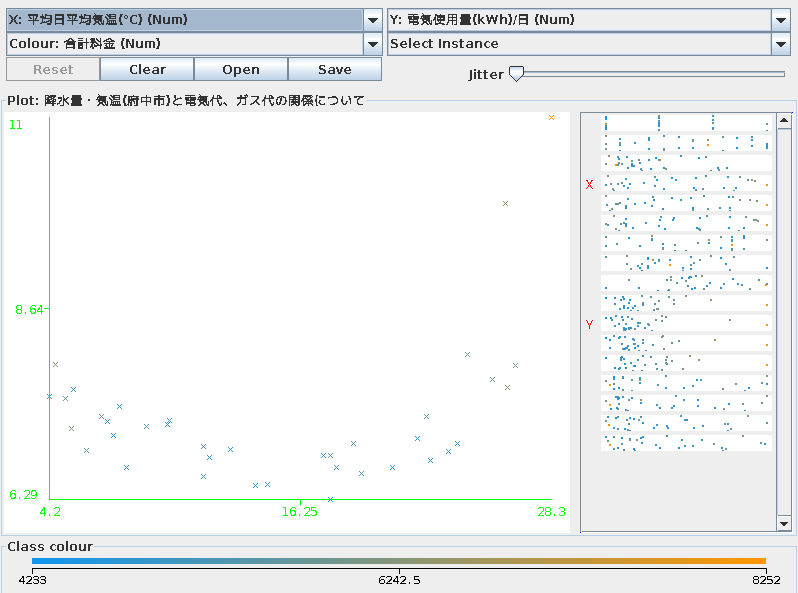
\includegraphics[width=1\hsize]{image201003/weka5.png}
 \caption{Visualize $B>\:Y2hLL(B}
\label{fig:wekavisualizedetail}
 \end{center}
\end{minipage}
\end{figure}


\subsubsection{$BJ,N`$7$F$_$k(B}

$B<!$KJ,N`$7$F$_$^$9!#(BClassify $B%?%V(B $B"*(B Choose $B%\%?%s$r2!$7!"I=<($5$l$?%D%j!<(B
$B$+$i(BMultilayer Perceptron ($B%K%e!<%i%k%M%C%H%o!<%/$K$h$kJ,N`(B)$B$rA*Br$7$^$9!#(B
$B<!$K!"(B(Num)$BJ?6QF|J?6Q5$29(B($B!n(B) $B$rL\E*4X?t$H$7$FA*Br$7$^$9!#(B
\index{neural network}

\begin{figure}[H]
\begin{center}
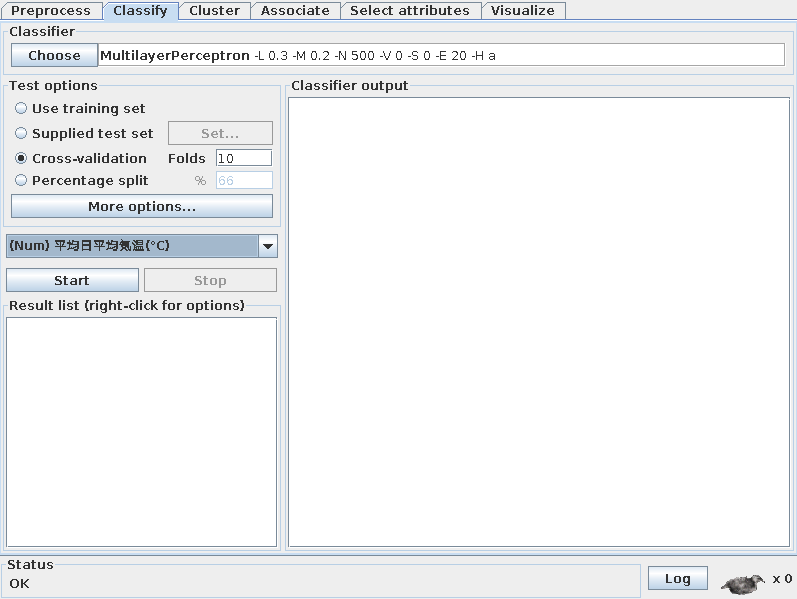
\includegraphics[width=0.6\hsize]{image201003/weka6.png}
\caption{Classify $B2hLL(B}
\end{center}
\end{figure}

Start $B%\%?%s$r%/%j%C%/$9$k$HJ,N`$,<B9T$5$l!"7k2L$,I=<($5$l$^$9!#(B

\begin{figure}[H]
\begin{center}
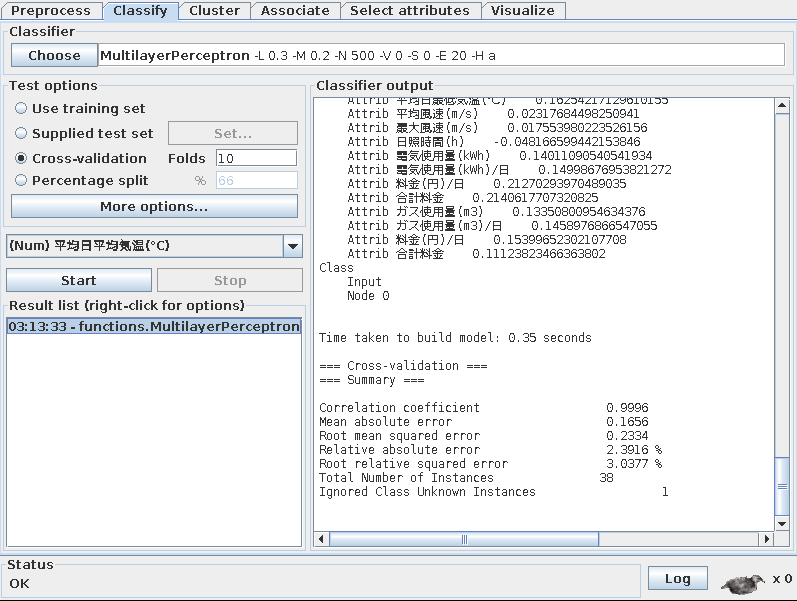
\includegraphics[width=0.6\hsize]{image201003/weka7.png}
\caption{Classify $B7k2L(B}
\end{center}
\end{figure}

\subsubsection{$BM=B,$7$F$_$k(B}

$B<B$O!"(Bkohnetsu.arff $B$N:G8e$N9T(B(2010$BG/(B3$B7n$N%G!<%?(B)$B$O!"$[$H$s$I$N9`L\$r(B'?'$B$rF~NO(B
$B$7$F$$$^$9!#(B

\begin{commandline}
2010,3,?,?,?,?,?,?,?,?,?,?,?,?,?,?,?
\end{commandline}

$B$3$l$O$^$@:#7n$N%G!<%?$,=P$F$$$J$$$+$i$G$9!#$=$l$G$O!"$3$l$i$rM=B,$7$F$_(B
$B$^$9!#@h$[$I$N(B Classify $B%?%V$N2hLL$G(B More options $B$r%/%j%C%/$7!"(BOutput
predictions $B$N%A%'%C%/$rF~$l!"(BOK $B$r2!$7$^$9!#(B

\begin{figure}[H]
\begin{center}
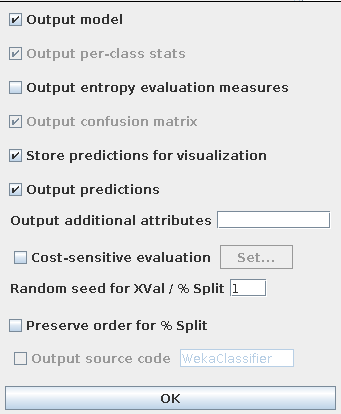
\includegraphics[width=0.4\hsize]{image201003/weka8.png}
\caption{Classify $B$N(B More Options $B%@%$%"%m%0(B}
\end{center}
\end{figure}

Start $B$r<B9T$9$k$H!"M=B,7k2L$,I=<($5$l$^$9!#(Bactual $B$,<B%G!<%?$G(B
predicted $B$,M=B,7k2L$G$9!#:#2s8+$?$$$N$O!"(B3$B7n$NJ?6QF|J?6Q5$29$G$9!#(B
actual $B$,(B ? $B$K$J$C$F$$$k9T$N!"(Bpredicted $B$NCM$r8+$k$H!"(B15.436 $B$H$J$C$F$$(B
$B$^$9!#2a5nFI$_9~$^$;$?%G!<%?$+$i%K%e!<%i%k%M%C%H%o!<%/$G$NJ,@O$7$FM=B,$7(B
$B$?7k2L!"$*$=$i$/0lF|$"$?$j$NJ?6Q5$29$O(B 15.4 $B!n(B $B$K$J$k$H$$$&M=B,$G$9!#Mh(B
$B7n!"5$>]D#$NE}7W%G!<%?$,99?7$5$l$?$i3NG'$7$F$_$^$7$g$&!#(B

\begin{figure}[H]
\begin{center}
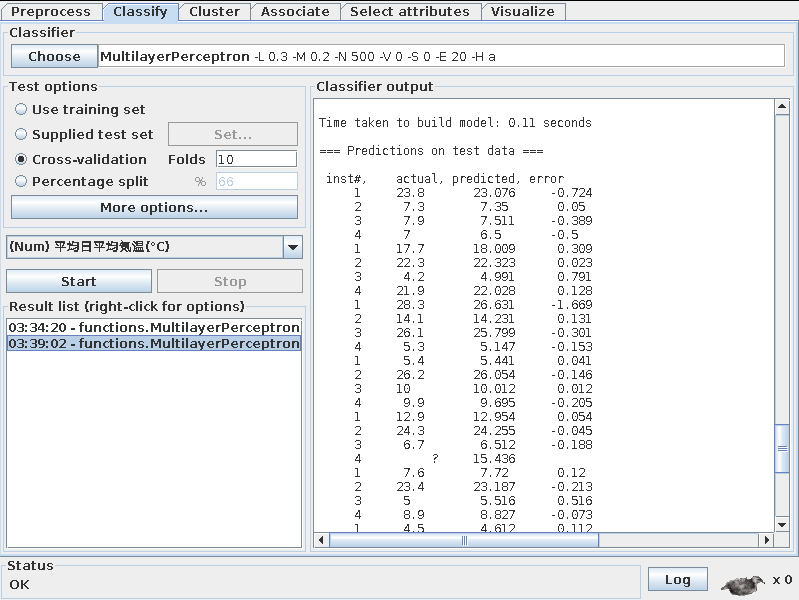
\includegraphics[width=0.6\hsize]{image201003/weka9.png}
\caption{$BM=B,7k2L(B}
\end{center}
\end{figure}

\subsection{$B$^$H$a(B}

$B$J$s$H$J$/;H$($=$&$J5$$,$7$?$G$7$g$&$+!#;d$O$3$l$GKh7n$N%,%9Be!"EE5$Be!"(B
$B$5$i$K$O?eF;Be$NM=B,$r$7$F!"5kM?F|A0F|$NM=;;7W2h$KMxMQ$7$F$$$3$&$H;W$$$^(B
$B$9!#;E;v$G$b!"4k2h>e$NN"IU$1%G!<%?$NJ,@O!"M=B,$J$I$K$b;H$($=$&$G$9$M!#(B

\subsection{$B;29MJ88%(B}
\begin{itemize}
 \item \url{http://www.ilibrary.jp/MOTtextBooks/text/weka.pdf}
 \item \url{http://web.sfc.keio.ac.jp/~soh/dm03/}
 \item \url{http://www1.doshisha.ac.jp/~mjin/R/23.pdf}
 \item \url{http://weka.wikispaces.com/ARFF}
\end{itemize}

%-------------------------------------------------------------------------------
% from debianmeetingresume201003.tex
\dancersection{Debian $B$G(B libfftw $B$r;H$C$F$_$k(B}{$B>e@n=c0l(B}
%-------------------------------------------------------------------------------
\index{fftw}
\index{FFT}
\index{DFT}
\index{libfftw}
\index{libsndfile}

\subsection{$B$O$8$a$K(B}

Debian$B$G(BFFT$B$r<h$j07$&(BC$B$N%"%W%j%1!<%7%g%s$r=q$$$F$_$?$$$H;W$&$3$H$O$"$j(B
$B$^$;$s$+(B?$B:#F|$O2;@<%G!<%?$rJ,@O$7$F$_$^$7$g$&!#(B

wav $B%U%!%$%k$rF~NO$H$7$F<u$1<h$j!"(BFFT$B$r<B9T$7$F$=$N7k2L$rI=<($9$k%"%W%j%1!<(B
$B%7%g%s$r:n@.$7$F$_$^$9!#(B

\subsection{$B%$%s%9%H!<%k(B}

libfftw3 $B$r%$%s%9%H!<%k$7$^$9!#(B
$B$"$H!"2;@<%U%!%$%k$r%m!<%I$9$k$?$a$K(B sndfile1 $B$rMxMQ$7$^$9!#(B

\begin{commandline}
$ apt-get install libfftw3-dev libsndfile1-dev
\end{commandline}
%$

\subsection{$B<B83BP>]$N=`Hw(B:$B4JC1$J(Bsine$BGH$r:n@.$9$k(B}

$B$^$:!"%F%9%HMQ$K(BFFT$B$N7k2L$,M=A[$G$-$k%G!<%?$r:n@.$7$F$_$^$9!#(B
$B$3$3$G$O(B 440Hz $B$N$-$l$$$J%5%$%sGH$r:n@.$7$F$$$^$9!#(B

\begin{equation*}
 data(x) = sin (\frac{2 \pi 440 x}{44100} ) 
\footnote{sin $B$O(B radian}
\end{equation*}

\begin{commandline}
/*BINFMTC: -lsndfile -lm

  Create a sine wave at 44.1kHz for 1 second called sine.wav
 */
#include <stdlib.h>
#include <stdio.h>
#include <sndfile.h>
#include <math.h>

int create_sine(const char* filename, int size, double frequency)
{
  SF_INFO sfinfo = {
    .frames = size,
    .samplerate = 44100,
    .channels = 1,
    .format = SF_FORMAT_WAV | SF_FORMAT_PCM_16,
    .sections = 0,
    .seekable = 0
  };
  SNDFILE* s = sf_open(filename, SFM_WRITE, &sfinfo);
  double* data = malloc(sizeof(double) * size);
  int i;

  for (i=0; i < size; ++i)
    {
      data[i] = sin(frequency * 2.0 * M_PI * i / 44100.0);
    }

  sf_writef_double(s, data, size);
  sf_close(s);
  return 0;
}

int main()
{
  return create_sine("sine.wav", 44100, 440.0);
}
\end{commandline}

\subsection{$B<B83BP>]$N=`Hw(B:$BJ#;($JF~NOCMNc$N=`Hw(B}

$B%F%9%HMQ$NF~NOCM$H$7$F!"E,Ev$J(B wav $B%U%!%$%k$rMQ0U$7$^$7$g$&!#(B

$B:#2s$O<j85$G!"(Baeolus $B$H$$$&%*%k%,%s%7%_%e%l!<%?$r5/F0$7!"(B 
jack $B$G@\B3$5$;!"(Becasound $B$r(B jack $BF~NO$K(B
$BBP$7$FBT5!$5$;!"(Bqjackctl $B$G@\B3$5$;$F<}O?$7$^$7$?!#(B

$B$=$l$J$j$KD9$$;~4VO?2;$7$?%G!<%?$+$i(B 16-bit mono $B$N(B PCM $B%G!<%?(B1$BICJ,$r@Z$j(B
$B=P$7$F<B83MQ%G!<%?$r:n@.$7$^$7$?!#(B

\begin{commandline}
$ qjackctl &
$ aeolus &
$ vkeybd &
$ ecasound -i jack -o test.wav
ctrl-C $B$GCfCG(B
$ sweep test.wav # $BE,Ev$KJT=8(B
$ file ra-mono.wav  # $B@Z$j=P$7$?7k2L$r3NG'(B
ra-mono.wav: RIFF (little-endian) data, WAVE audio, Microsoft PCM, 16 bit, mono 44100 Hz
\end{commandline}
%$

\subsection{FFTW$B$r;H$C$F(B wav $B%U%!%$%k$r=hM}$7$F$_$k(B}

sndfile $B$H(B fftw3 $B$r;H$C$F%U!<%j%(JQ49$7$F=PNO$r%@%s%W$7$F$_$^$7$g$&!#%5%s(B
$B%W%k%3!<%I$O(B sndfile $B$r;H$$(B double $B$NG[Ns$K(Bwav$B%U%!%$%k$NCf?H$rE83+$7$F!"(B
$B$=$NFbMF$r(B fftw $B$KEO$7$F=hM}$7$F$$$^$9!#(Bdouble $B$NCM$O3F(B 1/44100 $BIC$N=V4V(B
$B$K$*$1$k6u5$$N05NO$rI=$7$F$$$k$h$&$G$9!#(B

\begin{commandline}
/*BINFMTC: -lsndfile -lfftw3 -lm
 */

#include <stdlib.h>
#include <stdio.h>
#include <sndfile.h>
#include <math.h>
#include <complex.h>
#include <fftw3.h>

/*
  process with FFTW
 */
void study_sound(double* data, int size)
{
  fftw_complex* spectrum;
  fftw_plan p;
  int i;

  spectrum = (fftw_complex*) fftw_malloc(sizeof(fftw_complex) * (size / 2 + 1));
  p = fftw_plan_dft_r2c_1d(size, data, spectrum, FFTW_ESTIMATE);

  /* process with FFTW */
  fftw_execute(p);

  /* dump output in CSV format */
  printf("i,abs,arg\n");
  for (i=0; i<(size/2+1); ++i) {
    printf("%i,%f,%f\n", i,
	   cabs(spectrum[i]),
	   carg(spectrum[i]) / 2.0 / M_PI * 360.0);
  }
  fftw_destroy_plan(p);
  fftw_free(spectrum);
}

/*
  Process wav file.

  @return 1 on failure, 0 on success.
*/
int process_wav_file(const char* filename, int size)
{
  SF_INFO sfinfo = {0, 0, 0, 0, 0, 0};
  SNDFILE* s = sf_open(filename, SFM_READ, &sfinfo);
  double* data = malloc(sizeof(double) * size);

  if (!s || !data)
    {
      fprintf(stderr,
	      "Something went wrong opening the file or allocating memory\n");
      return 1;
    }
  if (sfinfo.channels != 1)
    {
      fprintf(stderr,
	      "Please give me monaural audio data\n");
      return 1;
    }

  /* Read wav file into an array of double */
  sf_readf_double(s, data, size / sfinfo.channels);
  study_sound(data, size / sfinfo.channels);
  sf_close(s);
  return 0;
}

int main(int argc, char** argv)
{
  process_wav_file(argv[1], atoi(argv[2]));
  return 0;
}
\end{commandline}

$B<B9T$7$F$_$^$9!#(B

\begin{commandline}
$ ./sndfile-fftw.c sine.wav 44100 > sine.csv
$ ./sndfile-fftw.c ra-1sec.wav 44100 > ra.csv
\end{commandline}
%$

\subsection{$B=PNO$r3NG'$7$F$_$k(B}

CSV$B%U%!%$%k7A<0$G%G!<%?$,=PNO$5$l$^$7$?!#(B
$B4JC1$K%0%i%U$r:n@.$9$k$?$a$N%D!<%k$H$7$F$3$3$G$O(BR$B$r;H$C$F$_$^$9!#(B

\begin{commandline}
$ R
> sine <- read.csv("sine.csv")
> ra <- read.csv("ra.csv")
> postscript("sine.eps", horizontal=FALSE, height=3, width=3)
> plot(sine$i, sine$abs, xlim=c(400,500), ylim=c(0,22000), type="l")
> dev.off()
> postscript("ra.eps", horizontal=FALSE, height=3, width=3)
> plot(ra$i, ra$abs, xlim=c(0,2000), ylim=c(0,100), type="l")
> dev.off()
\end{commandline}

\fgref{fig:wave-sine}$B$N(B440Hz $B$N%5%$%sGH$r=hM}$7$?7k2L$r8+$F$_$k$H!"(B440
Hz $B$"$?$j$K%0%i%U$NFM5/$,$"$k$N$,8+$F<h$l$^$9!#(B

$B$7$+$7!"<B:]$K%*%k%,%s2;$r=hM}$7$?7k2L$N(B\fgref{fig:wave-ra}$B$r8+$F$_$k$H!"(B
$B%0%i%U$KFM5/$,B??t$"$C$F!"7k9=J#;($G$9!#$=$N$^$^4JC1$K=hM}$5$;$F$/$l$O$7(B
$B$J$5$=$&$G$9!#(B

\begin{figure}[ht]
\begin{center}
 \begin{minipage}{0.4\hsize}
 \begin{center}
  \includegraphics{image201003/sine.eps}
 \end{center} 
 \label{fig:wave-sine}
 \caption{440Hz $B$N%5%$%sGH(B}
 \end{minipage}
 \begin{minipage}{0.4\hsize}
 \begin{center}
  \includegraphics{image201003/ra.eps}
 \end{center} 
 \label{fig:wave-ra}
 \caption{$B%i$r(Baeolus$B$GE,Ev$K1iAU$7$?2;(B}
 \end{minipage}
\end{center}
\end{figure}

%-------------------------------------------------------------------------------
% from debianmeetingresume201003.tex
\dancersection{man-db $B$r?<DI$$$7$?(B}{$BF|HfLn(B $B7<(B}
%-------------------------------------------------------------------------------
\index{man-db}
\index{groff}

\subsection{$BF|K\8l$N(Bman$B$,JQ(B}

$B$3$s$J46$8(B\\
\begin{wrapfigure}{r}{80mm}
\includegraphics[width=75mm]{image201003/manls.eps}
\end{wrapfigure}


$BF|K\8l$NJ8;z$NI=<(I}$,%"%k%U%!%Y%C%H$HF1$8$@$HH=Dj$5$l$F$7$^$C$F$$$k$N$G!"(B
$B7k2LE*$KF|K\8l$G=q$+$l$?9T$ND9$5$,G\$0$i$$$K$J$C$F$7$^$C$F$$$^$9!#(B

\subsection{$B2r$O(Bgroff$B$K$"$j(B}

\subsubsection{$B$=$b$=$b(Broff$B$C$F$I$&$$$&$b$N(B?}

$B4JC1$K8@$($P!"%?%$%W%i%$%?!<$N$h$&$J$b$N$G$9!#(B
$B$$$m$$$m$J%G%P%$%9$KBP$7$F0u;z$r9T$J$&$3$H$,$G$-$k%7%9%F%`$K$J$C$F$$$^$9$,!"(B
man$B$G$OJ8;zC<Kv$KJ8;z$NI}$H9b$5$r9MN8$7$J$,$i0u;z$r$7$F$$$-$^$9!#(B

\subsubsection{roff$BJ8;zI}$N;XDj(B}

$B0JA0$N%P!<%8%g%s$N(Bgroff$B$G$OF|K\8l$NJ8;z$NI=<(I}$,%"%k%U%!%Y%C%H$NG\$G$"$k$3$H$r(B
unicode$B$N(Bcode point$B$NHO0O$G@_Dj$7$F$"$j$^$7$?!#(B
groff$B$K$O$b$H$b$H(Bcode point$B$NHO0O$GJ8;z$NI}$r;XDj$9$k5!G=$,L5$$$?$a!"(B
$B$=$N5!G=$NDI2C$HF|K\8lJ8;z$NI=<(I}$rG\$K$9$k%Q%C%A$,$"$F$F$"$j$^$7$?!#(B

$B99?7$5$l$?%P!<%8%g%s$K$*$$$F$OF|K\8lBP1~$N%Q%C%A$,Ev$?$i$J$/$J$C$F$7$^$C$F$$$^$9$,!"(B
$B$d$O$jF1MM$NBP=h$r9T$J$&I,MW$,$"$j$=$&$G$9!#(B

% $B:G6a$O$=$NF|K\8l$NJ8;z$NI}$N;XDj$,=@Fp$K$J$C$?$h$&$G$9$,!"@5$7$$@_Dj$,$5(B
% $B$l$F$$$J$$$h$&$G$9!#(B

% =======================================================================
% from debianmeetingresume201002.tex
\dancersection{Debian$B$N(BOCaml$B4D6-$G3+H/$9$k4X?t7?8@8l%$%s%?%W%j%?(B}{$BF|HfLn(B $B7<(B}
\index{functional programming}
\index{OCaml}
\index{Haskell}
% =======================================================================

\subsection{OCaml$B$O$I$s$J8@8l(B}

$B@EE*7?$N7??dO@8@8l$H$$$&$N$,:#$N;d$NG'<1$G$9!#(B
$B4X?t7?8@8l$i$7$$5!G=$,CmL\$5$l$^$9$,!"$=$l0J30$N%9%?%$%k$bNI$/MxMQ$5$l$^$9!#(B

$B$3$3$G$O$3$N5-;v$rFI$_$9$9$a$k$K$"$?$C$FI,MW$=$&$J(BOCaml$B$N5!G=$K$D$$$F4JC1$K>R2p$7$^$9!#(B

\subsubsection{$BCM(B}

$B0J2<!"BPOC4D6-$NF~=PNO$rA0Ds$KOC$r$9$9$a$^$9!#(B

ocaml-interp$B%Q%C%1!<%8$N(B /usr/bin/ocaml $B$,BPOC4D6-$N%W%m%0%i%`$G$9!#(B

\verb|# | $B$OBPOC4D6-$N%W%m%s%W%H$G$9!#(B
$B%f!<%6!<$NF~NO$N=*$o$j$rBPOC4D6-$KG'<1$7$F$b$i$&$?$a$K(B \verb|;;|$B$rF~NO$7$^$9!#(B
$B$J$N$GBPOC4D6-$N(B\verb|# |$B%W%m%s%W%H$N8e$m$+$i(B\verb|;;|$B$^$G$,%f!<%6!<$NF~NO$G$9!#(B
\verb|- :|$B$+$i;O$^$kFbMF$OBPOC4D6-$N=PNO$G$9!#(B

\begin{commandline}
# 1;;
- : int = 1
# "abc";;
- : string = "abc"
# (1, "abc");;
- : int * string = (1, "abc")
# (1, ("abc", 2), 3);;
- : int * (string * int) * int = (1, ("abc", 2), 3)
# [ "a"; "b"; "c"];;
- : string list = ["a"; "b"; "c"]
# "a" :: "b" :: "c" :: [];;
- : string list = ["a"; "b"; "c"]
\end{commandline}

$BCM$rI=$9<0$rF~NO$9$k$HBPOC4D6-$O7?$NL>A0$HCM$r=PNO$7$F$$$^$9!#(B
\verb|1|$B$O(B\verb|int|$B7?!"(B\verb|"abc"|$B$O(B\verb|string|$B7?$H$J$C$F$$$^$9!#(B
$BBPOC4D6-$K<0$rF~NO$7$?$N$GI>2A$,9T$J$o$l!"$=$N7k2L$H$7$F$N=PNO$G$9!#(B

\verb|(1, ("abc", 2), 3)|$B$N$h$&$K%3%s%^$G6h@Z$C$F3g8L$G$/$/$C$?CM$O%?%W%k$G$9!#(B
$BCM$HCM$NAH$rI=8=$G$-$^$9!#7?$NL>A0$O(B \verb|*|$B$GO"$M$^$9!#G$0U$N7?$NCM$rAH$K$G$-$k6/NO$J5!G=$G$9!#(B

\verb|[ ]|$B$G%j%9%H$rI=8=$9$k$3$H$,$G$-$^$9!#$^$?!"(B\verb|::|$B$O(Blisp$B$G$$$&$H$3$m$N(Bcons$B$G$9!#(B
$B%j%9%H$NMWAG$OA4$FF1$87?$G$"$kI,MW$,$"$j$^$9!#(B

\subsubsection{$B%l%3!<%I$H%P%j%"%s%H(B}

$B<!$OCM$rI=8=$9$kA0$K$"$i$+$8$a7?$NDj5A$,I,MW$G$"$k$h$&$JCM$G$9!#(B

\begin{commandline}
# type vec_2d = { x : int; y : int };;
type vec_2d = { x : int; y : int; }
# { x = 1; y = 2 };;
- : vec_2d = {x = 1; y = 2}
# type int_or_string_or_none = I of int | S of string | N;;
type int_or_string_or_none = I of int | S of string | N
# I 3;;
- : int_or_string_or_none = I 3
# S "hello";;
- : int_or_string_or_none = S "hello"
# N;;
- : int_or_string_or_none = N
\end{commandline}

$B0l$DL\$NNc$O%l%3!<%I$G$9!#(BC$B$N9=B$BN$N$h$&$J$b$N$G!"%U%#!<%k%IL>$H%U%#!<%k%I$N7?$rDj5A$K5-=R$7$^$9!#(B
\verb|vec_2d|$B$H$$$&%l%3!<%I$N7?$rDj5A$7$F!"(B\verb|{ x = 1; y = 2 }|$B$H$$$&CM$rI>2A$5$;$^$7$?!#(B

$BFs$DL\$O%P%j%"%s%H$"$k$$$OBe?t%G!<%?7?$H8F$P$l$F$$$k<oN`$N7?$G$9!#(B
\verb|int_or_string_or_none|$B$H$$$&7?$rDj5A$7$F$$$F!"(B
$B$=$NCM$O(B I$B$H$$$&%?%0$NIU$$$?(Bint $B$+(B S$B$H$$$&%?%0$NIU$$$?(Bstring $B$+(B N $B$H$$$&%?%0(B $B$N$I$l$+$H$$$&$3$H$G$9!#(B
$B$3$N%?%0$N$3$H$r(B{\bf $B%3%s%9%H%i%/%?(B}$B$H8F$S$^$9!#(B

$B%P%j%"%s%H$O:F5"E*$JDj5A$b2DG=$G!"$3$N5!G=$G4JC1$KLZ9=B$$rI=8=$G$-$^$9!#(B

\begin{commandline}
# type str_tree = Leaf of string | Tree of (str_tree * str_tree);;
type str_tree = Leaf of string | Tree of (str_tree * str_tree)
# Leaf "abc";;
- : str_tree = Leaf "abc"
# Tree (Leaf "a", Tree (Leaf "b", Leaf "c"));;
- : str_tree = Tree (Leaf "a", Tree (Leaf "b", Leaf "c"))
\end{commandline}

\subsubsection{$B4X?t(B}

$B<!$O4X?t$rI=8=$9$kCM$G$9!#(B

\begin{commandline}
# (fun x -> x + 1);;
- : int -> int = <fun>
# (fun x -> x);;
- : 'a -> 'a = <fun>
\end{commandline}

\verb|(fun x -> x + 1)|$B$O4X?t$G$9!#(B
$B7?$,(B\verb|int -> int|$B$H=PNO$5$l$F$$$^$9$,!"(B
$B$3$l$O(Bint$B$r<u$1$H$C$F(Bint$B$rJV$94X?t$H$$$&0UL#$G$9!#(B
\verb|+|$B$N0z?t$O(Bint$B$H(Bint$B$J$N$G7k2L$H$7$F(B\verb|x|$B$O(B\verb|int|$B!"(B
\verb|fun x -> x + 1| $B$O(B \verb|int -> int|$B$H$$$&$h$&$K7?$N?dO@$,9T$J$o$l$F$$$^$9!#(B

$BFsHVL\$N(B\verb|(fun x -> x)|$B$b4X?t$G$9!#(B
$B7?$,(B\verb|'a -> 'a|$B$H=PNO$5$l$F$$$^$9$,!"(B
$B$3$l$O2?$+$"$k7?$NCM$r<u$1$H$C$F!"F1$87?$NCM$rJV$94X?t$H$$$&0UL#$G$9!#(B
$B$3$N(B \verb|'a -> 'a| $B$N4X?t$OG$0U$N7?$KBP$7$FE,MQ$,2DG=$J$N$G!"(B
$BA4$F$N7?$K$D$$$F$3$N4X?t$,Dj5A$5$l$F$$$k(B(\verb|int -> int| $B$b(B \verb|string -> string| $B$b(B ... etc)$B$N$HF1MM$N8z2L$,$"$j$^$9!#(B
$B$3$N$h$&$J7?$rB?Aj7?$H8F$S$^$9!#(B

\subsubsection{$BB+G{(B}

\verb|let|$B$r;H$C$FCM$rJQ?t$KB+G{$7$^$9!#(B
$B0J2<$O(B\verb|v|$B$K$?$$$7$F@0?t$r(B\verb|f|$B$KBP$7$F4X?t$rB+G{$7$F$$$^$9!#(B

\begin{commandline}
# let v = 123;;
val v : int = 123
# v;;
- : int = 123
# let f x y = (x + y) * (x - y);;
val f : int -> int -> int = <fun>
# f 5 3;;
- : int = 16
\end{commandline}

\subsubsection{$B%Q%?!<%s>H9g(B}

OCaml$B$OCM$N9=B$$rJ,2r$7$D$DJQ?t$rB+G{$9$k$3$H$,$G$-$^$9!#(B
$B<!$NNc$G$O%?%W%k$rJ,2r$7$FB+G{$r9T$J$C$F$$$^$9!#(B

\begin{commandline}
# let (x, y) = (2, 3 + 4);;
val x : int = 2
val y : int = 7
# let (a, (b, c)) = (1, (2, 3));;
val a : int = 1
val b : int = 2
val c : int = 3
\end{commandline}

\verb|match ... with|$B$r;HMQ$9$k$H!"9=B$J,2r$r;n$_$D$D>r7oJ,4t$9$k$3$H$,$G$-$^$9!#(B

$B4X?t(B\verb|len|$B$O%j%9%H$,6u$+$I$&$+$rH=Dj$7$J$,$i:F5"$7$F$$$^$9!#(B
$BB+G{$NDj5A;~$K<+?H$NDj5A$r;HMQ$9$k$H$-$K$O(B\verb|let|$B$G$O$J$/(B\verb|let rec|$B$r;H$$$^$9!#(B

$B4X?t(B\verb|what|$B$O@hDxDj5A$7$?%P%j%"%s%H(B\verb|int_or_string_or_none|$B$NCM$N<oN`$K$h$C$FJV$9J8;zNs$rJQ$($F$$$^$9!#(B

$B4X?t(B\verb|get_int|$B$O(B\verb|int_or_string_or_none|$B$,(Bint$B$N$H$-$@$1(BSome int$B$rJV$7!"$=$&$G$J$$$H$-$O(B None $B$rJV$7$^$9!#(B
'a option $B$OAH$_9~$_$N7?$G!"$"$k7?$NCM$,M-$k$+$"$k$$$OL5$$$+$rI=8=$G$-$k%P%j%"%s%H$G$9!#(B

\begin{commandline}
# let rec len ls = match ls with [] -> 0 | x :: rest -> 1 + len rest;;
val len : 'a list -> int = <fun>
# len [1; 2; 3];;
- : int = 3
# let what v = match v with I _ -> "int" | S _ -> "string" | N -> "none";;
val what : int_or_string_or_none -> string = <fun>
# what (S "abc");;
- : string = "string"
# what N;;
- : string = "none"
# let get_int v = match v with I i -> Some i | _ -> None ;;
val get_int : int_or_string_or_none -> int option = <fun>
# get_int N;;
- : int option = None
# get_int (I 10);;
- : int option = Some 10
\end{commandline}

\subsubsection{$B%b%8%e!<%k(B}

$B%W%m%0%i%`$N5,LO$,$*$*$-$/$J$C$F$/$k$HL>A06u4V$,=EMW$K$J$C$F$-$^$9!#(B
OCaml$B$K$O(Bmodule$B$N5!G=$,$"$jL>A06u4V$rJ,$1$k$3$H$,$G$-$^$9!#(B
$B$"$k%3%s%Q%$%kC10L$,(Bxyz.ml$B$H$$$&%U%!%$%kL>$@$C$?>l9g!"(B
$B$=$NCf$NDj5A$O(BXyz$B$H$$$&(Bmodule$B$NCf$KG[CV$5$l$^$9!#(B
$B%b%8%e!<%kFb$K$?$H$($P(Babc$B$H$$$&L>A0$,$"$C$?>l9g!"(B
$B8x3+$5$l$F$$$l$PB>$N%3%s%Q%$%kC10L$N%U%!%$%k$+$i$b(B Xyz.abc $B$H$$$&L>A0$G%"%/%;%9$9$k$3$H$,$G$-$^$9!#(B

\begin{commandline}
(* xyz.ml *)
let abc = "abc"
...


(* $BB>$N%U%!%$%k(B *)
... Xyz.abc ...
\end{commandline}

module$B$NCf$K$5$i$K(Bmodule$B$rDj5A$9$k$3$H$b$G$-$^$9!#(B
xyz.ml$B$NCf$K:n$C$?(Bmodule SubXyz$B$O!"(BXyz.SubXyz$B$H$$$&L>A0$N(Bmodule$B$G$9!#(B

$BDj5A:Q$_$N%b%8%e!<%k$r;H$C$F(Bmodule$B$rDj5A$9$k$3$H$b$G$-$^$9!#(B
$BAH$_9~$_$N(Bmodule$B$G$"$k(BList$B$r;H$C$F(B Xyz.L $B$rDj5A$7$F$$$^$9!#(B

\begin{commandline}
(* xyz.ml *)
module SubXyz =
  struct
  ...
  end

module L = List
\end{commandline}


\subsection{$B4X?t7?8@8l$N%$%s%?%W%j%?$N4JC1$J:n$j$+$?(B}

$B4X?t7?8@8l$H$O2?$G$7$g$&$+!#(B
$B$3$3$G$O4X?t$rCM$H$7$F$"$D$+$($k8@8l$H$$$&$3$H$K$7$F!"(B
$B$=$N$h$&$J8@8l$N%$%s%?%W%j%?$r:n$kOC$r$7$^$9!#(B

\subsubsection{$B4D6-$rEO$9%J%$!<%V$J%$%s%?%W%j%?<BAu(B}
\label{sec:envmach}

\paragraph{let$B$N4D6-(B} \ 

$BNc$($P0J2<$N$h$&$J%W%m%0%i%`$r9M$($^$9!#(B

\begin{commandline}
;; scheme function
(define (f)
  ;; env A
  (let ((x 1) (y 2) (z 3))
    ;; env B
    (let ((y 4))
      ;; env C
      (let ((z 5))
	;; env D
	(+ x y z)))))
\end{commandline}

\begin{commandline}
(* OCaml function *)
let f () =
  (* env A *)
  let (x, y, z) = (1, 2, 3) in
    (* env B *)
  let y = 4 in
    (* env C *)
  let z = 5 in
    (* env D *)
    x + y + z
\end{commandline}

$BJQ?t$NCM$N2r7h$N$?$a$N%F!<%V%k$r4D6-(B(environment)$B$H8F$V$3$H$K$7$F!"(B
$B<!$N?^$h$&$J9=B$$K$J$C$F$$$k$H9M$($F$_$^$9!#(B
$BJQ?t$N8!:w$O>e$+$i2<$K9T$J$o$l$k$H$9$k$H!"(B
$B$=$l$>$l$N%3%a%s%H$N0LCV$N4D6-$OLp0u$N0LCV$r;2>H$7$F$$$k$H9M$($F$h$$$O$:$G$9!#(B

 \includegraphics[height=0.3\hsize]{image201002/caml-env00.eps}\label{fig:env00}

\paragraph{$B4X?t8F$S=P$7$K$*$1$k4D6-(B} \ 

$B$5$i$K0J2<$N$h$&$J%W%m%0%i%`$r9M$($^$9!#(B

\begin{commandline}
(define (f x y)
  ;; env f
  (* x y 2))

;;env X

(let ((x 1) (y 2))
  (define (g)
    ;; env g
    (f 3 4))
  (g))

;;; may be another call of (f x y)
\end{commandline}

\begin{commandline}
let rec f x y =
  (* env f *)
  x * y * 2

(* env X *)

let (x, y) = (1, 2)
let rec g () =
  (* env g *)
  f 3 4

let v = g ()

(* may be another call of f x y *)
\end{commandline}

$B$9$k$H$=$l$>$l$N%3%a%s%H$N0LCV$N4D6-$O(B\fgref{fig:caml-env005}$B$N$h$&$K$J(B
$B$C$F$$$k$O$:$G$9!#(B

\begin{figure}[h]
 \centering
 \includegraphics[height=0.25\hsize]{image201002/caml-env005.eps}
 \caption{$B%3%a%s%H$N0LCV$N4D6-(B}
 \label{fig:caml-env005}
\end{figure}



$B$3$3$G4D6-(BX$B$OF1$84D6-$J$N$G!"6&M-$5$;$k$3$H$K$9$k$H<!$N$h$&$J9=B$$r9M$($k$3$H$,$G$-$^$9!#(B
$B$3$3$GCm0U$9$kI,MW$,$"$k$N$O!"4D6-(Bf$B$O4X?t(Bf$B$,8F$S=P$5$l$kEY$K0[$J$k$H$$$&$3$H$G$9!#(B
f$B$NDj5A0LCV$G$"$k4D6-(BX$B$O6&DL$G$9$,!"4D6-(Bf$B$O4X?t(Bf$B$,8F$S=P$5$l$kEY$K4D6-(BX$B$r;X$94D6-$r?-D9$9$kI,MW$,$"$j$^$9!#(B

 \includegraphics[height=0.5\hsize]{image201002/caml-env01.eps}

\paragraph{$B%/%m!<%8%c$N4D6-(B} \ 

$B0J2<$N$h$&$J%W%m%0%i%`$r9M$($^$9!#(B

\begin{commandline}
(define h
  (let ((x 1) (y 2))
    ;; env c
    (let ((f (lambda (z)
               ;; env l
	       (+ x y z))))
      f)))

;; env X

(h 3)
;;; may be another call of (h x)
\end{commandline}

\begin{commandline}
let rec h =
  let (x, y) = (1, 2) in
  (* env c *)
  let f z =
    (* env l *)
    x + y + z
  in f

(* env X *)

let v = h 3
(* may be another call of h x *)
\end{commandline}

$B4X?t$,JQ?t(Bh$B$KB+G{$5$l$F$$$^$9!#(B
$B$7$+$b(Bh$B$O(Bx, y$B$rB+G{$7$F$$$k(Blet$B$N30B&$K$"$k$K$b$+$+$o$i$:!"(B
$B8F$S=P$7$?:]$K$O(Bx, y$B$NCM$rI>2A$7$^$9!#(B

$B$3$N(Blet$B$N$h$&$J5!G=$r%l%-%7%+%k%9%3!<%W$H8F$S!"(B
$B$^$?$3$N$h$&$J4X?t$r%l%-%7%+%k%/%m!<%8%c(B(lexical closure)$B$"$k$$$OC1$K%/%m!<%8%c(B(closure)$B$H8F$S$^$9!#(B

$B>e$NNc$G$N4D6-$r9M$($F$_$k$H<!$N$h$&$J9=B$$K$J$C$F$$$k$O$:$G$9!#(B

 \includegraphics[height=0.5\hsize]{image201002/caml-env015.eps}

h$B$KB+G{$5$l$F$$$k(Bclosure$B$O$"$-$i$+$K4D6-(Bc$B$rCN$C$F$$$kI,MW$,$"$j$^$9!#(B
$B$J$<$J$i8F$S=P$7;~$K$O4D6-(Bc$B$r;X$94D6-$r@8@.$7$J$1$l$P$J$i$J$$$+$i$G$9!#(B
$B$7$?$,$C$F(Bclosure$B$O0J2<$N$h$&$J9=B$$K$J$C$F$$$k$H9M$($k$3$H$,$G$-$^$9!#(B
env$B$O(Bclosure$B$NDj5A0LCV$N4D6-$G(Bargs$B$O2>0z?t%j%9%H$=$7$F(Bbody$B$O4X?tK\BN$N<0$G$9!#(B

 \includegraphics[height=0.4\hsize]{image201002/caml-env02.eps}

$B<0$NI>2A$KI,MW$J4D6-$rI>2A4oFb$GEO$7$J$,$i!"(B
let$B$d4X?t8F$S=P$7$N:]$K$O4D6-$r?-D9$9$kJ}?K$r<h$k$H!"(B
$BHf3SE*4JC1$K%$%s%?%W%j%?$r<BAu$9$k$3$H$,$G$-$^$9!#(B
$B$^$?!"4D6-$rJ];}$9$k9=B$$r9M$($l$P(Bclosure$B$r<B8=$9$k$3$H$b$G$-$^$9!#(B

 $B;29M;qNA(B: \verb|http://www.sato.kuis.kyoto-u.ac.jp/~igarashi/class/isle4-05w/text/eopl003.html|

\subsection{OCaml$B$G$N(Blexing$B$H(Bparsing - ocamllex$B$H(Bocamlyacc}

\subsubsection{ocamllex}

ocamllex$B$O(BOCaml$B$KIUB0$7$F$$$k;z6g2r@O4X?t@8@.4o(B(lexer generator)$B$G!"(B
OCaml$B$+$i8F$S=P$;$k(Blexer$B$r@8@.$7$F$/$l$^$9!#(B
$B0J2<$N$h$&$K(BC$B8@8l$G$b$*$J$8$_$N(B lex, flex $B$H;w$?$h$&$J;HMQ46$K$J$C$F$$$^$9!#(B

\begin{commandline}

{
  (* header *)
  (* Lexing$B$N%k!<%kItJ,$G;2>H$7$?$$FbMF$r(BOCaml$B$G=q$/(B *)
}

(* $BJ8;zNs%Q%?!<%s$NDj5A(B *)

(* $B;z6g2r@O(B(lexing)$B$N%k!<%k5-=R(B *)

{
  (* trailer *)
  (* $B%k!<%kItJ,$G@8@.$5$l$?4X?t$r;2>H$9$kFbMF$r(BOCaml$B$G=q$/(B *)
}

\end{commandline}

\subsubsection{ocamlyacc}

$BF1MM$K!"(Bocamlyacc$B$O(BOCaml$B$KIUB0$7$F$$$k9=J82r@O4X?t@8@.4o(B(parser generator)$B$G!"(B
OCaml$B$+$i8F$S=P$;$k(Bparser$B$r@8@.$7$F$/$l$^$9!#(B
$B$3$A$i$b$d$O$j!"0J2<$N$h$&$K(B yacc, bison $B$H;w$?$h$&$J;HMQ46$K$J$C$F$$$^$9!#(B

\begin{commandline}

%{
  (* header *)
  (* $B9=J8LZ@8@.=hM}$G;2>H$7$?$$FbMF$r(BOCaml$B$G=q$/(B *)
%}
  /* declarations */
  /* $B=*C<5-9f$N7?$d9=J8LZ$N(Broot$B$N@k8@(B */
%%
  /* rules */
  /* $BJ8L.<+M3J8K!$H9=J8LZ@8@.=hM}$r5-=R(B */
%%
  (* trailer *)
  (* $B@8@.$5$l$?(Bparser$B$N4X?t$r;2>H$9$kFbMF$r(BOCaml$B$G=q$/(B *)

\end{commandline}

\subsubsection{ocamllex$B$H(Bocamlyacc$B$N;HMQNc(B}

ocamllex$B$H(Bocamlyacc$B$rJ;MQ$9$k>l9g$K$O!"(B
ocamlyacc$B$G@8@.$5$;$?(Bparser$B$N=*C<5-9f$NDj5A$r(B
lexer$B$+$i;2>H$5$;$k$h$&$K$9$k$N$,$b$C$H$bC1=c$J;H$$J}$G$9!#(B

$B0J2<$,(BS$B<0(Bparser$B$r@8@.$5$;$kNc$G$9!#(B
sParser.mly$B$r(Bocamlyacc$B$G=hM}$9$k$H(BsParser.ml$B$,@8@.$5$l!"(B
sLexer.mll$B$r(Bocamllex$B$G=hM}$9$k$H(BsLexer.ml$B$,@8@.$5$l$^$9!#(B

\par
\paragraph{sParser.mly}
$B7?$4$H$K=*C<5-9f$r(B\%token$B$G@k8@$7!"(B
\%start$B$H(B\%type$B$G9=J8LZ$N(Broot$B$H$=$N7?$r;XDj$7$^$9!#(B
root$B$NL>A0$,9=J82r@O4X?t$NL>A0$K$J$j$^$9!#(B

yacc$B$HF1$8MWNN$GJ8L.<+M3J8K!$r5-=R$7$F$$$-$^$9!#(B
expr$B$O??56CM!"?tCM!"J8;zNs$G$"$k$+!"(B
$B$"$k$$$O!"(Bexpr$B%I%C%HBP$^$?$O(Bexpr$B$rJB$Y$?$b$N(B $B$r3g8L$G3g$C$?$b$N$H$$$&Dj5A$K$J$C$F$$$^$9!#(B

\begin{commandline}

%{
  (* sParser.mly *)

  module C = SCons

%}

/* File sparser.mly */
%token LPAREN RPAREN DOT_SYMBOL EOL BOOL_TRUE BOOL_FALSE
%token <SCons.s_int> INT
%token <float> FLOAT
%token <string> SYMBOL
%token <string> STRING
%start expr
%type <SCons.s_expr> expr
%%

expr_list:
  { C.Null }
| expr DOT_SYMBOL expr { C.Cons($1, $3) }
| expr expr_list { C.Cons($1, $2) }

expr:
| BOOL_TRUE               { C.Bool(true) }
| BOOL_FALSE              { C.Bool(false) }
| INT                     { C.Int($1) }
| FLOAT                   { C.Float($1) }
| SYMBOL                  { C.Symbol($1) }
| STRING                  { C.String($1) }
| LPAREN expr_list RPAREN { $2 }

\end{commandline}

% $ dummy comment

\par
\paragraph{sLexer.mll}
$BJ8;zNs%Q%?!<%s$NDj5A$G$O!"@55,I=8=$NMWNN$GJ8;z=89g$d7+$jJV$7$NI=8=$rMxMQ$7$F(B
$BDj5A$r:n$j!"(Blet$B$GL>A0$rIU$1$F$$$-$^$9!#J8;z$r(B '' $B$G$/$/$k0J30$O@55,I=8=$HF1MM$G$9!#(B
$BDj5A$7$?J8;zNs%Q%?!<%s$r$5$i$KJL$NJ8;zNs%Q%?!<%s$K:FMxMQ$9$k$3$H$,$G$-$^$9!#(B

$B%k!<%k5-=R$NItJ,$G$O!"(Btoken$B$NJ8;zNs%Q%?!<%s$H(Btoken$B@8@.<0$r(Blex$B$NMWNN$G5-=R$7$F$$$-$^$9!#(B
$B%-!<%o!<%I(Brule$B$N8e$NJ8;zNs$,(Blexer$B$N4X?tL>$K$J$j$^$9!#$J$N$G$3$3$G$O$=$N4X?t$NL>A0$O(Btoken$B$G$9!#(B

$B;z6g2r@O(B(Lexing)$B$N2aDx$K$*$1$kF~NO%U%!%$%kFb$N0LCV$O!"(B
lexbuf$B$N(Blex\_start\_p$B$K5-9f(B(token)$B$N3+;O0LCV$,!"(B
lex\_curr\_p$B$K(Btoken$B$N=*N;$N<!$N0LCV$,J];}$5$l$F$$$^$9!#(B
ocamllex$B%G%U%)%k%H$NF0:n$G$O(Bpos\_cnum $B%U%#!<%k%I$,99?7$5$l$k$N$_$J$N$G!"(B
$B%U%!%$%k@hF,$+$i$N%P%$%H?t$7$+$o$+$j$^$;$s!#(B
$BM[$K9T?t$NG'<1$d%?%V$K$h$k%+%i%`?t$NJd@5$r9T$J$&>l9g$K$O!"(B
lex\_start\_p$B$H(Btoken$B$r$b$H$K(Blex\_curr\_p$B$r=$@5$7$F$d$kI,MW$,$"$j$^$9!#(B
\footnote{$B<!$N(Blex\_start\_p$B$O8=:_$N(Blex\_curr\_p$B$+$i0z$-7Q$,$l$k$N$G!"(B
lex\_curr\_p$B$r=$@5$9$l$P==J,$G$9!#(B}



\begin{commandline}
{
  (* sLexer.mll*)

  module LX = Lexing
  module P = SParser
  ... (* $BCfN,(B *)
  let fix_position lexbuf =
    let newline pos = {
      pos with
	LX.pos_lnum = pos.LX.pos_lnum + 1;
	LX.pos_cnum = pos.LX.pos_cnum + 1;
	LX.pos_bol = pos.LX.pos_cnum + 1;
    } in

    let tab pos = {
      pos with
	LX.pos_cnum = pos.LX.pos_cnum + 8 - (pos.LX.pos_cnum - pos.LX.pos_bol) mod 8
    } in

    let other pos = {
      pos with
	LX.pos_cnum = pos.LX.pos_cnum + 1
    } in

    let rec fix_pos_rec pos str =
      let len = (String.length str) in
	match (if len > 0 then (Some (str.[0]), String.sub str 1 (len - 1))
	       else (None, "")) with
	    (None, _) -> pos
	  | (Some '\n', rest) -> fix_pos_rec (newline pos) rest
	  | (Some '\t', rest) -> fix_pos_rec (tab pos) rest
	  | (Some _, rest) -> fix_pos_rec (other pos) rest
    in
    let _ = lexbuf.LX.lex_curr_p <- fix_pos_rec (LX.lexeme_start_p lexbuf) (LX.lexeme lexbuf) in
      ()
}

/* $BJ8;zNs%Q%?!<%s$NDj5A(B */
let str_esc = '\\'
let double_quote = '"'
let str_escaped_char = str_esc _
let str_char = [^ '\\' '"']
let str = double_quote (str_char | str_escaped_char)* double_quote

let left_paren = '('
let right_paren = ')'
let space = [' ' '\t' '\n' '\r']+
let dot_symbol = '.'
let bool_true  = '#' 't'
let bool_false = '#' 'f'

let int = '-'? ['0' - '9']+
let float = '-'? ['0' - '9']+ '.' ['0' - '9']* | '-'? ['0' - '9']* '.' ['0' - '9']+
let symbol = [^ '"' '(' ')' ' ' '\t' '\n' '\r']+

/* lexing$B$N%k!<%k5-=R(B */
rule token = parse
  | left_paren      { P.LPAREN }
  | right_paren     { P.RPAREN }
  | space      { fix_position lexbuf; token lexbuf }
  | dot_symbol      { P.DOT_SYMBOL }
  | bool_true       { P.BOOL_TRUE }
  | bool_false      { P.BOOL_FALSE }
  | int      { expr_integer (LX.lexeme lexbuf) }
  | float    { P.FLOAT(Pervasives.float_of_string(LX.lexeme lexbuf)) }
  | symbol   { P.SYMBOL(LX.lexeme lexbuf) }
  | str      { fix_position lexbuf; P.STRING(expr_string(LX.lexeme lexbuf)) }
  | eof      { raise Eof }

\end{commandline}

%\pagebreak

\subsection{Haskell$B$N(BLexing}

Haskell$B$K$O(B
$B%V%m%C%/$N3+;O$d=*N;$N(Btoken$B$d<0$N6h@Z$j$N(Btoken$B$r>JN,$9$k$3$H$,$G$-$k(B
layout rule$B$H$$$&5!G=$,$"$j$^$9!#(B
$B$=$N$?$a>JN,$5$l$?(Btoken$B$r(Blexing$B$N2aDx$GJd$C$F$d$kI,MW$,$"$j$^$9!#(B

$B$^$:!"DL>o$HF1MM$K(Blexing$B$r9T$J$C$F(Btoken$BNs$r@8@.$7!"(B
$B$=$N(Btoken$BNs$K5,B'$K=>$C$F(Btoken$B$rJd$&$H$$$&$h$&$K!"(B2$BCJ3,$N9)Dx$r9T$J$$$^$9!#(B

\subsubsection{layout$B$J$7$N(BLexing}

\paragraph{lexer0.mll header$BItJ,(B} \ 

$B$^$:$O(B.mll$B$N(Bheader$BItJ,$G$9!#(B

$B8e$+$i(Blayout rule$B$K$*$$$FI,MW$H$J$k%+%i%`?t$r?t$($"$2$k=hM}$?$a$K0LCV>pJs$N=$@5$r9T$J$&4X?t(B(fix\_position)$B$rDj5A$7$F$$$^$9!#(B
$B$^$?!"(BHaskell$B$NJ8;z$*$h$SJ8;zNs%j%F%i%k$O%j%F%i%kFb$N%k!<%k$,J#;(EY$N9b$$;EMM$J$N$G!"(B
$BJL$N(Blexer($B8e=R(B)$B$r8F$S=P$7$D$D<B:]$NJ8;zNsI=8=$r9=@.$9$k4X?t(B(decode\_char, decode\_string)$B$r=`Hw$7$F$$$^$9!#(B


\paragraph{fix\_position $B0LCV>pJs$N=$@5(B} \ 
\begin{commandline}
{
  (* lexer0.mll header$BItJ,(B *)
  module LX = Lexing
  module P = Parser
  ... (* $BCfN,(B *)
  let fix_position lexbuf =
    let newline pos =
      { pos with
          LX.pos_lnum = pos.LX.pos_lnum + 1;
          LX.pos_cnum = pos.LX.pos_cnum + 1;
          LX.pos_bol = pos.LX.pos_cnum + 1;
      } in

    let tab pos =
      { pos with
          LX.pos_cnum = pos.LX.pos_cnum + 8 - (pos.LX.pos_cnum - pos.LX.pos_bol) mod 8
      } in

    let other pos =
      { pos with
          LX.pos_cnum = pos.LX.pos_cnum + 1
      } in

    let rec fix_pos_rec pos str =
      let len = (String.length str) in
        match (if len > 0 then (Some (str.[0]), String.sub str 1 (len - 1))
               else (None, "")) with
            (None, _) -> pos
          | (Some '\n', rest) -> fix_pos_rec (newline pos) rest
          | (Some '\t', rest) -> fix_pos_rec (tab pos) rest
          | (Some _, rest) -> fix_pos_rec (other pos) rest
    in
    let _ = lexbuf.LX.lex_curr_p <- fix_pos_rec (LX.lexeme_start_p lexbuf) (LX.lexeme lexbuf) in
      ()
  ... (* $BCfN,(B *)
\end{commandline}

\pagebreak

\paragraph{decode\_char, decode\_string $BJ8;z$*$h$SJ8;zNs%G%3!<%@!<(B} \
\begin{commandline}
  ... (* $BCfN,(B *)
  let decode_cexpr cexpr =
    let fchar = String.get cexpr 0 in
    let escexp = String.sub cexpr 1 ((String.length cexpr) - 1) in
    let fmatch exp str = Str.string_match (Str.regexp exp) str 0 in
      if fchar = '\\' then
        match escexp with
            "NUL"   -> Some '\x00'
          | "SOH" | "^A"   -> Some '\x01'
          | "STX" | "^B"   -> Some '\x02'
        ... (* $BCfN,(B *)
          | "RS"  | "^^"   -> Some '\x1e'
          | "US"  | "^_"   -> Some '\x1f'
          | "SP"           -> Some ' '

          | "\\"           -> Some '\\'
          | "\""           -> Some '"'
          | "'"            -> Some '\''

          | "DEL"          -> Some '\x7f'

          | _ when fmatch "^[0-9]+$" escexp
              -> Some (Char.chr (int_of_string escexp))
          | _ when fmatch "^[xX][0-9a-zA-Z]+$" escexp 
              -> Some (Char.chr (int_of_string ("0" ^ escexp)))
          | _ when fmatch "^[oO][0-7]+$" escexp
              -> Some (Char.chr (int_of_string ("0" ^ escexp)))

          | _ -> None

      else Some fchar

  let decode_char lexbuf =
    let cstr = LX.lexeme lexbuf in
    let len = String.length cstr in
      match decode_cexpr (String.sub cstr 1 (len - 2)) with
          Some c -> c
        | None   -> failwith (F.sprintf "Unkown char expression %s" cstr)

  let decode_string lexbuf =
    let sexpr = LX.lexeme lexbuf in
    let len = String.length sexpr in
    let strlbuf = Lexing.from_string (String.sub sexpr 1 (len - 2)) in
    let rec decode result =
      match HsStr.char strlbuf with
          HsStr.Eos -> result
        | HsStr.Char cstr ->
            if cstr = "\\&" then decode (result ^ "&")
            else decode (result ^ 
                           match (decode_cexpr cstr) with
                               None -> failwith (F.sprintf "Unkown char expression '%s' in literal string" cstr)
                             | Some c -> (String.make 1 c))
        | HsStr.Gap g -> decode result
    in decode ""
}
\end{commandline}

% $ dummy comment

\pagebreak

\paragraph{lexer0.mll $BJ8;zNs%Q%?!<%sDj5AItJ,(B} \ 

$B<!$KJ8;zNs%Q%?!<%s$NDj5A$G$9!#(B

$B9T?t$O$A$g$C$HB?$$$G$9$,!"FC$KFq$7$$$H$3$m$O$"$j$^$;$s!#(B
$BLdBj$N%j%F%i%kJ8;zNs$G$9$,!"%j%F%i%kJ8;zNsItJ,$NJ8;zNs%Q%?!<%s<+BN$OLdBj$J$/I=8=$G$-$F$$$^$9!#(B
$B$7$+$7!"%j%F%i%k$GI=8=$5$l$kJ8;zNs<+BN$rI|85$9$k$N$,J#;($J$N$GA05-$*$h$S8e=R$N$h$&$J=`Hw$,I,MW$K$J$j$^$9!#(B

\begin{commandline}
/* lexer0.mll $BJ8;zNs%Q%?!<%sDj5AItJ,(B */
let special = ['(' ')' ',' ';' '[' ']' '`' '{' '}']

let space = ' '
let newline = ("\r\n"|['\n' '\r'])
let tab = '\t'

let dashes = '-' '-' '-'*

let ascSmall = ['a'-'z']
let small = ascSmall | '_'
let ascLarge = ['A'-'Z']
let large = ascLarge

let plus = '+'
let minus = '-'
let exclamation = '!'
let ascSymbol_nbs = [ '!' '#' '$' '%' '&' '*' '+' '.' '/' '<' '=' '>' '?' '@' '^' '|' '-' '~' ]
let ascSymbol = ascSymbol_nbs | '\\'
let symbol = ascSymbol

let ascDigit = ['0'-'9']
let digit = ascDigit

let octit = ['0'-'7']
let hexit = ascDigit | ['a'-'z' 'A'-'Z']

let decimal = (digit)+
let octal = (octit)+
let hexadecimal = (hexit)+

let exponent = ['e' 'E'] ['+' '-']? decimal
let float = decimal '.' decimal exponent? | decimal exponent

let graphic = small | large | symbol | digit | special | [':' '"' '\'']
let any = graphic | space | tab

let comment = dashes ((space | tab | small | large | symbol | digit | special | [':' '"' '\'']) (any)*)? newline

let whitechar = newline | space | tab
let whitestuff = whitechar | comment 
let whitespace = (whitestuff)+

(*
let lwhitechar = space | tab
let lwhitestuff = lwhitechar | comment 
let lwhitespace = (lwhitestuff)+
*)

let char_gr = small | large | ascSymbol_nbs | digit | special | [':' '"']
let str_gr  = small | large | ascSymbol_nbs | digit | special | [':' '\'']

let charesc = ['a' 'b' 'f' 'n' 'r' 't' 'v' '\\' '"' '\'']
let str_charesc = charesc | '&'
let cntrl = ascLarge | ['@' '[' '\\' ']' '^' '_']
let gap = '\\' (whitechar)+ '\\'
(* let gap = '\\' (lwhitechar | newline)+ '\\' *)

let ascii = ('^' cntrl) | "NUL" | "SOH" | "STX" | "ETX" | "EOT" | "ENQ" | "ACK"
  | "BEL" | "BS" | "HT" | "LF" | "VT" | "FF" | "CR" | "SO" | "SI" | "DLE"
  | "DC1" | "DC2" | "DC3" | "DC4" | "NAK" | "SYN" | "ETB" | "CAN"
  | "EM" | "SUB" | "ESC" | "FS" | "GS" | "RS" | "US" | "SP" | "DEL"

let escape = '\\' ( charesc | ascii | decimal | 'o' octal | 'x' hexadecimal )
let str_escape = '\\' ( str_charesc | ascii | decimal | 'o' octal | 'x' hexadecimal )

let char = '\'' (char_gr | space | escape) '\''
let string = '"' (str_gr | space | str_escape | gap)* '"'

let varid = small (small | large | digit | '\'')*
let conid = large (small | large | digit | '\'')*

let varsym = symbol (symbol | ':')*
let consym = ':' (symbol | ':')*

let modid = conid
\end{commandline}

% $ dummy comment

\pagebreak

\paragraph{lexer0.mll $B%k!<%k5-=RItJ,(B} \ 

$B:G8e$K%k!<%k5-=R$G$9!#(B

$B%9%Z!<%9!"%?%V!"2~9T$J$I$r4^$s$G$$$k(Bwhitespace$B$d(Bstring$B$N$H$3$m$G(B
fix\_position$B$r8F$s$G0LCV>pJs$rJd@5$7$F$$$^$9!#(B
$B$^$?(Bchar$B$d(Bstring$B$N%j%F%i%k$+$iJ8;z$dJ8;zNs$r9=@.$9$k$?$a$K(B
decode\_char, decode\_string $B$r8F$S=P$7$F$$$^$9!#(B

\begin{commandline}
(* lexer0.mll $B%k!<%k5-=RItJ,(B *)
rule token = parse
  | '('  { P.SP_LEFT_PAREN(loc lexbuf) }
  | ')'  { P.SP_RIGHT_PAREN(loc lexbuf) }
  | ','  { P.SP_COMMA(loc lexbuf) }
  | ';'  { P.SP_SEMI(loc lexbuf) }
  | '['  { P.SP_LEFT_BRACKET(loc lexbuf) }
  | ']'  { P.SP_RIGHT_BRACKET(loc lexbuf) }
  | '`'  { P.SP_B_QUOTE(loc lexbuf) }
  | '{'  { P.SP_LEFT_BRACE(loc lexbuf) }
  | '}'  { P.SP_RIGHT_BRACE(loc lexbuf) }
      (** special tokens *)

  | "case"     { P.K_CASE(loc lexbuf) }
  | "class"    { P.K_CLASS(loc lexbuf) }
  | "data"     { P.K_DATA(loc lexbuf) }
  | "default"  { P.K_DEFAULT(loc lexbuf) }
  | "deriving" { P.K_DERIVING(loc lexbuf) }
  | "do"       { P.K_DO(loc lexbuf) }
  | "else"     { P.K_ELSE(loc lexbuf) }
  | "if"       { P.K_IF(loc lexbuf) }
  | "import"   { P.K_IMPORT(loc lexbuf) }
  | "in"       { P.K_IN(loc lexbuf) }
  | "infix"    { P.K_INFIX(loc lexbuf) }
  | "infixl"   { P.K_INFIXL(loc lexbuf) }
  | "infixr"   { P.K_INFIXR(loc lexbuf) }
  | "instance" { P.K_INSTANCE(loc lexbuf) }
  | "let"      { P.K_LET(loc lexbuf) }
  | "module"   { P.K_MODULE(loc lexbuf) }
  | "newtype"  { P.K_NEWTYPE(loc lexbuf) }
  | "of"       { P.K_OF(loc lexbuf) }
  | "then"     { P.K_THEN(loc lexbuf) }
  | "type"     { P.K_TYPE(loc lexbuf) }
  | "where"    { P.K_WHERE(loc lexbuf) }
  | "_"        { P.K_WILDCARD(loc lexbuf) }
      (** reservedid *)

  | ".."       { P.KS_DOTDOT(loc lexbuf) }
  | ":"        { P.KS_COLON(loc lexbuf) }
  | "::"       { P.KS_2_COLON(loc lexbuf) }
  | "="        { P.KS_EQ(loc lexbuf) }
  | "\\"       { P.KS_B_SLASH(loc lexbuf) }
  | "|"        { P.KS_BAR(loc lexbuf) }
  | "<-"       { P.KS_L_ARROW(loc lexbuf) }
  | "->"       { P.KS_R_ARROW(loc lexbuf) }
  | "@"        { P.KS_AT(loc lexbuf) }
  | "~"        { P.KS_TILDE(loc lexbuf) }
  | "=>"       { P.KS_R_W_ARROW(loc lexbuf) }
      (** reservedop *)

  | "as"              { P.K_AS(loc lexbuf) }  (** maybe varid *)
  | "qualified"       { P.K_QUALIFIED(loc lexbuf) }  (** maybe varid *)
  | "hiding"          { P.K_HIDING(loc lexbuf) }  (** maybe varid *)
  | varid      { P.T_VARID(LX.lexeme lexbuf, loc lexbuf) }
  | conid      { P.T_CONID(LX.lexeme lexbuf, loc lexbuf) }
      (** identifiers or may be qualified ones *)

  | whitespace  { fix_position lexbuf; P.WS_WHITE(loc lexbuf) }  (** comment begining with dashes is not varsym *)
      (** white spaces *)

  | plus       { P.KS_PLUS(loc lexbuf) }  (** maybe varsym *)
  | minus      { P.KS_MINUS(loc lexbuf) } (** maybe varsym *)
  | exclamation  { P.KS_EXCLAM(loc lexbuf) } (** maybe varsym *)
  | varsym     { P.T_VARSYM(LX.lexeme lexbuf, loc lexbuf) }
  | consym     { P.T_CONSYM(LX.lexeme lexbuf, loc lexbuf) }
      (** symbols or may be qualified ones *)

  | modid '.' varid   { P.T_MOD_VARID(decode_with_mod lexbuf, loc lexbuf) }
  | modid '.' conid   { P.T_MOD_CONID(decode_with_mod lexbuf, loc lexbuf) }
  | modid '.' varsym  { P.T_MOD_VARSYM(decode_with_mod lexbuf, loc lexbuf) }
  | modid '.' consym  { P.T_MOD_CONSYM(decode_with_mod lexbuf, loc lexbuf) }
      (** qualified xx *)

  | char      { P.L_CHAR(decode_char lexbuf, loc lexbuf) }
  | string    { fix_position lexbuf; P.L_STRING(decode_string lexbuf, loc lexbuf) }

  | decimal | ('0' ['o' 'O'] octal) | ('0' ['x' 'X'] hexadecimal)
        { P.L_INTEGER(Int64.of_string(LX.lexeme lexbuf), loc lexbuf) }

  | float      { P.L_FLOAT(float_of_string(LX.lexeme lexbuf), loc lexbuf) }

  | eof        { P.EOF(loc lexbuf) }
  ... /* $B0J2<N,(B */
\end{commandline}


\paragraph{hsStr.mll} \ 

$BJ8;zNs$N(Blexer$B$G$9!#(B

$B$3$3$G$N(Btoken$B$OJ8;zNs%j%F%i%kFb$N(B1$BJ8;z$NI=8=$"$k$$$O%.%c%C%W(B(gap)$B$G$9!#(B
Haskell$B$G$O(B1$B$D$NJ8;zNs%j%F%i%k$rCfCG$7$F!"(B
$B4V$K6uGr$d2~9T$d%3%a%s%H$r5-=R$7$?8e$K!":F3+$9$k$3$H$,$G$-$^$9!#(B
$B$3$N6uGr$d2~9T$d%3%a%s%H$NItJ,$,(Bgap$B$G$9!#(B

$B$3$3$GDj5A$5$l$?(Bchar$B4X?t$rMxMQ$7$F(Bdecode\_string$B4X?t$OJ8;zNs$r9=@.$7$F$$$/$h$&$K$J$C$F$$$^$9!#(B

\begin{commandline}
{
  (* hsStr.mll *)
  module LX = Lexing

  type ct =
      Char of string
    | Gap of string
    | Eos
}

let special = ['(' ')' ',' ';' '[' ']' '`' '{' '}']

let space = ' '
let newline = ("\r\n"|['\n' '\r'])
let tab = '\t'

let ascSmall = ['a'-'z']
let small = ascSmall
let ascLarge = ['A'-'Z']
let large = ascLarge

let ascSymbol_nbs = [ '!' '#' '$' '%' '&' '*' '+' '.' '/' '<' '=' '>' '?' '@' '^' '|' '-' '~' ]

let ascDigit = ['0'-'9']
let digit = ascDigit

let octit = ['0'-'7']
let hexit = ascDigit | ['a'-'z' 'A'-'Z']

let decimal = (digit)+
let octal = (octit)+
let hexadecimal = (hexit)+

let lwhitechar = space | tab

let str_gr  = small | large | ascSymbol_nbs | digit | special | [':' '\'']

let charesc = ['a' 'b' 'f' 'n' 'r' 't' 'v' '\\' '"' '\'']
let str_charesc = charesc | '&'
let cntrl = ascLarge | ['@' '[' '\\' ']' '^' '_']
let gap = '\\' (lwhitechar | newline)+ '\\'

let ascii = ('^' cntrl) | "NUL" | "SOH" | "STX" | "ETX" | "EOT" | "ENQ" | "ACK"
  | "BEL" | "BS" | "HT" | "LF" | "VT" | "FF" | "CR" | "SO" | "SI" | "DLE"
  | "DC1" | "DC2" | "DC3" | "DC4" | "NAK" | "SYN" | "ETB" | "CAN"
  | "EM" | "SUB" | "ESC" | "FS" | "GS" | "RS" | "US" | "SP" | "DEL"

let str_escape = '\\' ( str_charesc | ascii | decimal | 'o' octal | 'x' hexadecimal )

rule char = parse
  | str_gr | space | str_escape  { Char(LX.lexeme lexbuf) }
  | gap                          { Gap(LX.lexeme lexbuf) }
  | eof                          { Eos }
\end{commandline}

% $ dummy comment

$B;29M;qNA(B: \verb|http://www.sampou.org/haskell/report-revised-j/lexemes.html|

\subsubsection{Haskell$B$N(Blayout rule}

$B$3$N@a$N;O$a$K$b=q$$$?$h$&$K(Blayout rule$B$O!"(B
token$BNs$K$5$i$K(Btoken$B$rJd$C$F$d$k=hM}$G$9!#(B
$B$^$:$OJd$&%k!<%k$r3NG'$7$F$_$^$7$g$&!#(B
$B0J2<$K!"(BHaskell 98 Language Report$B$N2~D{HG$NOBLu(B
\footnote{http://www.sampou.org/haskell/report-revised-j/syntax-iso.html\#layout}$B$+$i0zMQ$7$F$_$^$9!#(B

%%\paragraph{--- $B0zMQ$3$3$+$i(B ---} \ 

\dotfill $B0zMQ$3$3$+$i(B\dotfill

%% \par
%% \begin{tabular}{c|c|c}
%% \cline{1} & $B0zMQ$3$3$+$i(B & \cline{3} \\
%% \end{tabular}

 $B%l%$%"%&%H$N1F6A$O!"$3$N@a$G$O!"%l%$%"%&%H$rMQ$$$F$$$k%W%m%0%i%`$K!"$I$N$h$&$K$7$F!"%V%l!<%9$H%;%_%3%m%s$rDI2C$9$k$+$r5-=R$9$k$3$H$K$h$C$F;XDj$9$k!#$3$N;EMM$O!"JQ49$r9T$&4X?t(B L $B$N7A$r$H$k!#(BL  $B$X$NF~NO$O(B

\begin{itemize}

    \item $B$3$N(B Haskell $B%l%]!<%H$N;z6g9=J8$G;XDj$5$l$?$h$&$J;z6g$NJB$S$G!"0J2<$N$h$&$JDI2C%H!<%/%s$,$D$$$F$$$k$b$N!#(B

    \begin{itemize}
          \item $B%-!<%o!<%I(B let$B!"(Bwhere$B!"(Bdo $B$"$k$$$O(B of $B$N$"$H$K;z6g(B \{ $B$,B3$+$J$$>l9g!"%H!<%/%s(B $\{n\}$ $B$r%-!<%o!<%I$N8e$KA^F~$9$k!#$3$3$G(B n $B$O!"$b$7<!$N;z6g$,$"$l$P$=$l$N%$%s%G%s%H!"$^$?$O!"%U%!%$%k$N=*C<$KE~C#$7$F$$$l$P(B 0 $B$G$"$k!#(B
          \item $B%b%8%e!<%k$N:G=i$N;z6g$,(B \{ $B$"$k$$$O(B module $B$G$O(B $B$J$$$H$-!"$=$N;z6g$NA0$K(B $\{n\}$ $B$rCV$/!#$3$3$G!"(Bn $B$O$=$N;z6g$N%$%s%G%s%H$G$"$k!#(B
          \item $BF10l9T$G!";z6g$N3+;O$NA0$K$OGr6uGr$7$+$J$$$H$-!"$3$N;z6g$NA0$K(B $<n>$ $B$rCV$/!#$3$3$G(B n $B$O$3$N;z6g$N%$%s%G%s%H$G!"(B $BA0$NFs$D$N5,B'$N7k2L!"$=$NA0$K$O(B $\{n\}$ $B$,CV$+$l$F$$$J$$!#(B ($BCm0U(B: $BJ8;zNs%j%F%i%k$OJ#?t9T$K$^$?$,$k$3$H$,$"$k(B -- 2.6 $B@a!#$7$?$,$C$F!"(B
\begin{commandline}
              f = ("Hello \
                      \Bill", "Jake")
\end{commandline}
            $B$G$O!"(B\verb|\Bill| $B$NA0$K(B $<n>$ $B$OA^F~$5$l$k$3$H$O$J$$!#$J$<$J$i!"40A4$J;z6g$N3+;O>l=j$G$O$J$$$+$i$@!#$^$?!"(B, $B$NA0$K$b(B $<n>$ $B$OCV$+$l$k$3$H$O$J$$!#$J$<$J$i!"$=$NA0$K(B $BGr6uGr0J30$N$b$N$,$"$k$+$i$@!#(B)
    \end{itemize}

    \item$B!V%l%$%"%&%HJ8L.!W$N%9%?%C%/$N$=$l$>$l$NMWAG$O0J2<$N$I$l$+$G$"$k!#(B

    \begin{itemize}
          \item $B%<%m!"$3$l$OJ8L.$rL@<(E*$K0O$&$3$H(B($B$?$H$($P%W%m%0%i%^$,3+%V%l!<%9(B $B$rMQ0U$7$?>l9g(B)$B$r<($9!#$b$7:G$bFbB&$NJ8L.$,(B 0 $B$J$i!"0O$^$l$?J8L.$,(B $B=*N;$9$k$+!"?7$7$$J8L.$,%W%C%7%e$5$l$k$^$G!"%l%$%"%&%H%H!<%/%s$OA^(B $BF~$5$l$J$$!#(B
          \item $B@5$N@0?t!"$3$l$O0O$^$l$?%l%$%"%&%HJ8L.$N%$%s%G%s%H%+%i%`?t(B
    \end{itemize}

\end{itemize}

$B;z6g$N!V%$%s%G%s%H!W$O;z6g$N:G=i$NJ8;z$N%+%i%`?t$G$"$k!#(B
$B$R$H$D$N9T$N%$%s%G%s%H$H$O:G$b:8$K$"$k;z6g$N%$%s%G%s%H$rI=$9!#(B
$B$3$N%+%i%`?t$r7hDj$9$k$?$a$K0J2<$N$h$&$J5,Ls$r$b$D8GDjI}$N%U%)%s%H$r2>Dj$9$k!#(B

\begin{itemize}
    \item $B2~9T!"%j%?!<%s!"%i%$%s%U%#!<%I$*$h$S%U%)!<%`%U%#!<%IJ8;z$O$9$Y$F?7$7$$9T$r3+;O$9$k(B
    \item $B:G=i$N%3%i%`$O(B 0 $B$G$O$J$/(B 1 $B$G$"$k(B
    \item $B%?%V%9%H%C%W$O(B8$BJ8;zJ8$:$D$N0LCV$K$"$k(B
    \item $B%?%VJ8;z$O8=:_0LCV$+$i<!$N%?%V%9%H%C%W0LCV$^$G$=$m$($k$N$KI,MW$J$@$1$N6uGr$rA^F~$9$k!#(B
\end{itemize}

$B%l%$%"%&%H%k!<%k$K$"$o$;$k$?$a$K!"%=!<%9%W%m%0%i%`Cf$N(B Unicode $BJ8;z$O(B ASCII $BJ8;z$HF1$8I}$N8GDjI}$G$"$k$H4GJo$9!#$7$+$7$J$,$i!"8+$?L\$H$N:.(B $BMp$rHr$1$k$?$a%W%m%0%i%^$O0EL[$N%l%$%"%&%H$N0UL#$,Hs6uGrJ8;z$NI}$K0M(B $BB8$9$k$h$&$J%W%m%0%i%`$r=q$+$J$$$h$&$K$9$Y$-$G$"$k!#(B

\paragraph{$BE,MQ(B} \ 

L tokens [ ] $B$O!"(Btokens $B$N%l%$%"%&%H$K4XCN$7$J$$JQ49$r$b$?$i$9!#(B
$B$3$3$G!"(Btokens $B$O%b%8%e!<%k$N;z6g2r@O$*$h$S>e=R$N$h$&$K%+%i%`?tI=<(;R$rDI2C$7$?7k2L$G$"$k!#(B
L $B$NDj5A$O0J2<$N$H$*$j!"$3$3$G$O(B $B!V(B:$B!W$r%9%H%j!<%`9=C[A`:n;R$H$7$F;H$$!"!V(B[ ]$B!W$O6u$N%9%H%j!<%`$G$"$k!#(B

\begin{commandline}
L (<n>:ts) (m:ms)   = ; : (L ts (m:ms))  if m = n
                    = } : (L (<n>:ts) ms) if n < m
L (<n>:ts) ms       = L ts ms
L ({n}:ts) (m:ms)   = { : (L ts (n:m:ms)) if n > m   (Note 1)
L ({n}:ts) []       = { : (L ts [n]) if n > 0        (Note 1)
L ({n}:ts) ms       = { : } : (L (<n>:ts) ms)        (Note 2)
L (}:ts) (0:ms)     = } : (L ts ms)                  (Note 3)
L (}:ts) ms         = parse-error                    (Note 3)
L ({:ts) ms         = { : (L ts (0:ms))              (Note 4)
L (t:ts) (m:ms)     = } : (L (t:ts) ms) if m /= 0 and parse-error(t)  (Note 5)
L (t:ts) ms         = t : (L ts ms)
L [] []             = []
L [] (m:ms)         = } : L [] ms if m /=0           (Note 6)
\end{commandline}


%% \paragraph{Note 1.}

%% $BF~$l;R$K$J$C$?J8L.$O!"0O$^$l$?J8L.(B ($n>m$) $B$h$j$b?<$/%$%s%G(B $B%s%H$5$l$F$$$J$1$l$P$J$i$J$$!#(B
%% $B$5$b$J$1$l$P!"(BL $B$O<:GT$7!"$^$?!"%3%s%Q%$%i$O%l%$%"%&%H%(%i!<$rI=<($7$J$1$l$P$J$i$J$$!#$?$H$($P!"(B

%% \begin{commandline}
%%   f x = let
%%            h y = let
%%     p z = z
%%                  in p
%%         in h
%% \end{commandline}

%% $B$3$3$G!"(Bp $B$NDj5A$O0O$^$l$?J8L.$N%$%s%G%s%H$h$j$b@u$$%$%s%G%s%H$G$"$k!#(B
%% $B$3$N>l9g!"(Bh $B$NDj5A$K$h$C$F@_Dj$5$l$k!#(B

%% \paragraph{Note 2.}

%% where $B$N8e$N:G=i$N%H!<%/%s$,!"$?$H$($P!"0O$^$l$?J8L.$h$j$b%$%s%G%s%H$5$l$F$$$k$N$G$J$1$l$P!"(B
%% $B$=$N%V%m%C%/$O6u$G$J$1$l$P$J$i$J$$!#(B 
%% $B$@$+$i!"6u$N%V%l!<%9$,A^F~$5$l$k!#(B
%% $B%H!<%/%s(B $\{n\}$ $B$O(B $<n>$ $B$KCV$-49(B $B$($i$l!"6u$N%V%l!<%9$,L@<(E*$K$J$C$F$$$?>l9g$N>u67$rLOJo$9$k!#(B

%% \paragraph{Note 3.}

%% $B8=:_$N%l%$%"%&%HJ8L.$K$D$$$F(B 0 $B$KBP$7$F>H9g$9$k$3$H$G!"(B
%% $BL@<(E*$JJD%V%l!<%9$,L@<(E*$J3+%V%l!<%9$K$N$_BP1~$9$k$3$H$r3N$+$a$k!#(B
%% $B$b$7!"L@<(E*(B $B$JJD%V%l!<%9$,0EL[$N3+%V%l!<%9$KBP1~$7$F$$$k>l9g$K$O9=J82r@O%(%i!<$H$J$k!#(B

%% \paragraph{Note 4.}

%% $B$3$l$O!"$9$Y$F$N%V%l!<%9$NBP$OL@<(E*$J%l%$%"%&%HJ8L.$H$7$F07$o$l$k$3$H$r0UL#$7!"(B
%% $B%i%Y%kIU$N%G!<%?9=C[$*$h$S99?7(B (3.15 $B@a(B)$B$r4^$`!#$3$3$K$3$N7A<02=$H(B Haskell 1.4 $B$G$N0c$$$,$"$k!#(B

%% \paragraph{Note 5.}

%% $BI{<!E*$J>r7o(B parse-error(t) $B$O<!$N$h$&$K2r<a$5$l$k!#(B
%% $B$b$7!"<!$N(B $B%H!<%/%s$,(B t $B$G$"$k$h$&$J(B L $B$K$h$C$F@8@.$5$l$?%H!<%/%s$,(B Haskell $B$NJ8K!$NIT@5$J@\F,<-$rI=$o$7$F$$$k>l9g!"(B
%% $B$*$h$S!"(B $B!V(B\}$B!W%H!<%/%s$,B3$/(B L $B$K$h$C$F@8@.$5$?%H!<%/%s$N(B Haskell $BJ8K!$N@5$7$$@\F,<-$G$"$k>l9g!"(Bparse-error(t) $B$O??$H$J(B $B$k!#(B

%% $m /= 0$ $B$N%A%'%C%/$O!"0EL[$KDI2C$5$l$?JD%V%l!<%9$,!"0EL[$N3+%V%l!<%9$K(B $BBP1~$9$k$3$H$r$?$7$+$a$k!#(B

%% \paragraph{Note 6.}

%% $BF~NO$N=*C<$K$*$$$F!"J]N1$5$l$?JD%V%l!<%9$,$9$Y$FA^F~$5$l$k!#(B
%% $B$3$N;~E@(B $B$G%l%$%"%&%HJ8L.$N$J$+$K$"$k(B($B$9$J$o$A!"(B$m = 0$ $B$G$"$k(B)$B$H%(%i!<$H$J$k!#(B


\dotfill $B0zMQ$3$3$^$G(B $B0J2<N,(B \dotfill

$B$@$$$VD9$/$J$C$F$7$^$C$?$N$G(B Note $B$O>JN,$G$9!#(B

$B$o$+$j$K$/$$$G$9$,!"$3$3$G$bFbItE*$K$O(B2$BCJ3,$K$J$C$F$$$^$9!#(B

$B$^$:85$N(Btoken$BNs$K0l$DL\$NA`:n$rE,MQ$7$^$9!#0J2<$N$h$&$J5,B'$@$H9M$($k$H$o$+$j$d$9$$$+$b$7$l$^$;$s!#(B

\begin{itemize}
 \item let, where, do, of $B$N8e$K(B \{ $B$,L5$$>l9g$K$OBe$o$j$K%V%m%C%/$N3+;O$r$"$i$o$9(B token $\{n\}$ $B$rA^F~!#(B
 \item $B%U%!%$%k$N@hF,$b%b%8%e!<%k@k8@$,>JN,$5$l$F$$$F(B \{ $B$,L5$$>l9g$K$O(B token $\{n\}$ $B$G%V%m%C%/3+;O!#(B
 \item $B%$%s%G%s%H$N%l%Y%k$G8e$+$i%V%m%C%/$rG'<1$9$k$?$a$K(B token $<n>$ $B$rA^F~$7$F$*$/!#(B
\end{itemize}

$B$D$.$KFs$DL\$NA`:n$G$"$k4X?t(B L $B$rE,MQ$7$^$9!#(B

L $B$O$b$H$N(Btoken$BNs$H%$%s%G%s%H%l%Y%k$N%9%?%C%/$r0z?t$K$H$j!"(B
$B$b$H$N(Btoken$BNs$K(Btoken$B$rA^F~$7$?$b$N$rJV$94X?t$G$9!#(B
$B$d$O$j0J2<$N$h$&$J5,B'$@$H9M$($k$H$o$+$j$d$9$$$+$b$7$l$^$;$s!#(B

\begin{itemize}
 \item $B%$%s%G%s%H%l%Y%k(B$<n>$ $B$,F1$8%l%Y%k$N%V%m%C%/Fb$G$"$l$P(B($B%9%?%C%/;2>H(B) ; $B$rA^F~$7$F<0$r=*N;!"%V%m%C%/$r7QB3(B
 \item $B%$%s%G%s%H%l%Y%k(B$<n>$$B$NJ}$,@u$1$l$P(B \} $B$rA^F~$7$F%V%m%C%/$r=*N;(B
 \item $B%$%s%G%s%H%l%Y%k(B$<n>$$B$,$"$C$F>e$N$I$A$i$G$b$J$1$l$P<0$r7QB3(B

 \item $B$"$k%V%m%C%/Fb$G(B($B%9%?%C%/;2>H(B)$B$h$j%$%s%G%s%H%l%Y%k$N?<$$%V%m%C%/3+;O(B$\{n\}$$B$,$"$C$?$i(B \{ $B$rA^F~$7%V%m%C%/$r3+;O!#(B
$B%V%m%C%/3+;O$r$"$i$o$9%$%s%G%s%H%l%Y%k(Bn$B$r%9%?%C%/$K@Q$`(B
 \item $B%V%m%C%/3+;O(B $\{n\}$ $B$,:G$b30B&$G$bF1MM$K%V%m%C%/3+;O!#(B \{ $B$rA^F~$7!"(Bn$B$r%9%?%C%/$K@Q$`(B
 \item $B%V%m%C%/3+;O(B $\{n\}$ $B$,$"$C$F>e$N$I$A$i$G$b$J$1$l$P(B \{ $B$*$h$S(B \} $B$rA^F~$76u$N%V%m%C%/$r:n$k!#(B
$B<B$O%V%m%C%/3+;O$G$O$J$+$C$?$H$$$&$3$H$,$3$3$G$o$+$k$N$GBe$o$j$K(B $<n>$ $B$rA^F~$9$k!#(B

 \item \} $B$,$"$C$?$i%9%?%C%/$+$i(B 0 $B$r<h$j=P$9(B
 \item \} $B$,$"$C$F(B 0 $B$r9_$m$;$J$+$C$?$i(B parse error

 \item \{ $B$,$"$C$?$i%9%?%C%/$K(B 0 $B$r@Q$`(B

 \item $B>e$N$I$l$G$b$J$/!"$^$?%V%m%C%/Fb$G$"$j!"%V%m%C%/$r7QB3$9$k$H(B parse error $B$K$J$k$H$-$O(B \} $B$rA^F~$7$F%V%m%C%/$rJD$8$k!#(B
 \item $B>e$N$I$l$G$b$J$/!"$^$?%V%m%C%/Fb$G$"$k$H$-$O(B parse error $B$K$J$i$J$$8B$j%V%m%C%/$r7QB3!#(B
 \item $B%H!<%/%s$b%9%?%C%/$b6u$J$i$*$o$j(B
 \item $B%H!<%/%s$,6u$G%9%?%C%/$K(B 0 $B$G$J$$CM$,;D$C$F$$$k$J$i(B \} $B$rA^F~$7$F%9%?%C%/$+$i<h$j=P$9!#(B( 0$B$,$"$C$?$i%(%i!<(B )
\end{itemize}

$B;29M;qNA(B: \verb|http://www.sampou.org/haskell/report-revised-j/syntax-iso.html#layout|


\paragraph{OCaml$B$G$N<BAu(B} \ 

$B!V(Bparse error $B$K$J$i$J$$8B$j%V%m%C%/$r7QB3!W$N%k!<%k$O$+$J$j<BAu$,$d$C$+$$$G$7$?!#(B%%$B$3$l$O(Bparser$B$N$H$3$m$G8e=R$7$^$9!#(B
$B:#2sMxMQ$7$?(Bocamlyacc$B$O(Byacc$B$d(Bbison$B$HF1$8$h$&$K(BLALR(1)$B$N(Bparser generator$B$H$J$C$F$*$j!"(B
$B4pK\E*$K$O(Btoken$BNs$rESCf$^$GFI$_9~$s$@0LCV$H$=$N(Btoken$B$*$h$S0l$D@h$N(Btoken$B$K$h$C$F9=J82r@OCf$N<!$NF0:n$r7hDj$7$F$$$^$9!#(B
$B$3$3$G=P$F$-$?$h$&$J(B parse error $B$K$J$k$^$G%V%m%C%/$,JD$8$k$+$o$+$i$J$$$h$&$J;EMM$H$O$"$^$jAj@-$,NI$/$"$j$^$;$s!#(B
backtrack$B$r9T$J$($k$h$&$J(Bparser$B$J$i$3$N$h$&$J;EMM$KBP$7$F$b$h$j4JC1$KBP1~$G$-$k$H9M$($i$l$^$9!#(B
$B:#2s$O(Btoken$BNs$N(Btoken$B$4$H$K(Bparse error$B$N%U%i%0$rIU2C$7$F$d$j$J$*$7$r9T$J$&$3$H$GBP1~$7$^$7$?!#(B
$B<B9T8zN($O$h$/$"$j$^$;$s$,LdBj$K$J$k$[$I(Btoken$B?t$,B?$/$J$i$J$1$l$PBg>fIW$=$&$G$9!#(B
$B>-MhE*$K$O(BPackrat parsing$B$N$h$&$JJ}K!$G(Bparser$B$r=q$-D>$7$F$_$?$$$H$3$m$G$9!#(B

OCaml$B$G>e(Blayout rule$B$r<BAu$7$?4X?t$,<!$N$h$&$J46$8$G$9!#(B
token$BNs$X$N0l$DL\$NA`:n$HFs$DL\$NA`:n$r=gHV$K:\$;$F$$$^$9!#(B
P.BLK\_OPEN $B$,(B $\{n\}$ $B$G(B P.BLK\_LEVEL $B$,(B $<n>$ $B$K$"$?$k$b$N$G$9!#(B
$B$b$H$NDj5A$H;w$?$h$&5-=R$GI=8=$G$-$F$$$k$N$,$o$+$k$G$7$g$&$+!#(B

%%\paragraph{token$BNs$X$NA`:n(B 1$B$DL\(B} \ 
\begin{commandline}
let all_token_rev_list lexbuf =
  let unget_s = S.create () in
  let get_token () = L0.token lexbuf in
  let blk_level_pair tk =
    let loc = L0.get_location tk in (loc.T.start_p.T.col + 1, loc) in
  let eof_token_p = (function P.EOF(_) -> true | _ -> false) in

  let rec scan_start () =
    match get_token () with
        (P.SP_LEFT_BRACE _ | P.K_MODULE _) as start -> start
      | P.WS_WHITE _ -> scan_start ()
      | other ->
          let _ = S.push other unget_s in
            P.BLK_OPEN (blk_level_pair other)
  in

  let scan_next prev = 
    let rec scan_next_rec () =
      let cur =
        if (S.is_empty unget_s) then (get_token ())
        else (S.pop unget_s) in

        match (prev, cur) with
            (_, (P.EOF(_) as eoft)) -> eoft
          | (_, P.WS_WHITE(_)) -> (scan_next_rec ())
          | ((P.K_LET(_) | P.K_WHERE(_) | P.K_DO(_) | P.K_OF(_)), (P.SP_LEFT_BRACE(_) as lbr)) -> lbr
          | ((P.K_LET(_) | P.K_WHERE(_) | P.K_DO(_) | P.K_OF(_)), tk) ->
              let (_, (level, loc)) = (S.push tk unget_s, blk_level_pair tk) in
                P.BLK_OPEN((if (eof_token_p tk) then 0 else level), loc)
          | (_, tk) ->
              let (_, loc) as p = blk_level_pair tk in
                if (loc.T.start_p.T.line
                    - (L0.get_location prev).T.end_p.T.line) > 0 then
                  let _ = S.push tk unget_s in P.BLK_LEVEL p
                else tk
    in (scan_next_rec ())
  in
    (LST.fold_left
       (fun r a -> ((a, new_err_flag ()) :: r))
       []
       (LST.create_stream (scan_start ()) scan_next eof_token_p))
\end{commandline}

%%\paragraph{token$BNs$X$NA`:n(B 2$B$DL\(B} \ 
\begin{commandline}
let rec layout istream levels =
  let push_new_token tok lform =
    LST.Cons ((tok, new_err_flag ()), lform)
  in

  let (tok, err) =
    match LST.peek istream with
        None -> raise Parsing.Parse_error
      | Some x -> x
  in
    match (tok, levels) with
        ((P.BLK_LEVEL (n, loc)), (m :: mstl as ms)) when m = n ->
          let addtk = P.SP_SEMI(loc) in
            push_new_token addtk (lazy (layout (LST.tl istream) ms))
      | ((P.BLK_LEVEL (n, loc)), m :: ms) when n < m  ->
          push_new_token (P.SP_RIGHT_BRACE(loc)) (lazy (layout istream ms))
      | ((P.BLK_LEVEL (n, _)), ms)                         -> layout (LST.tl istream) ms
      | ((P.BLK_OPEN (n, loc)), (m :: ms as levels)) when n > m  ->
          push_new_token (P.SP_LEFT_BRACE(loc)) (lazy (layout (LST.tl istream) (n :: levels))) (* Note 1 *)
      | ((P.BLK_OPEN (n, loc)), []) when n > 0             ->
          push_new_token (P.SP_LEFT_BRACE(loc)) (lazy (layout (LST.tl istream) [n])) (* Note 1 *)
      | ((P.BLK_OPEN (n, loc)), ms)                        ->
          push_new_token
            (P.SP_LEFT_BRACE(loc))
            (lazy (push_new_token
                     (P.SP_RIGHT_BRACE(loc))
                     (lazy (layout (push_new_token
                                      (P.BLK_LEVEL(n, loc))
                                      (lazy (LST.tl istream))) ms)))) (* Note 2 *)
      | ((P.SP_RIGHT_BRACE _ as rbr), 0 :: ms)        ->
          LST.Cons ((rbr, err), lazy (layout (LST.tl istream) ms)) (* Note 3 *)
      | ((P.SP_RIGHT_BRACE _), ms)                   -> raise Parsing.Parse_error (* Note 3 *)
      | ((P.SP_LEFT_BRACE _ as lbr), ms)             -> 
          LST.Cons ((lbr, err), lazy (layout (LST.tl istream) (0 :: ms))) (* Note 4 *)

      | ((P.EOF loc as eoft), [])                    -> LST.Cons ((eoft, err), lazy (LST.Nil))
      | ((P.EOF loc), m :: ms) when m <> 0           -> 
          push_new_token (P.SP_RIGHT_BRACE(loc)) (lazy (layout istream ms)) (* Note 6 *)

      | (t, (m :: mstl)) when m <> 0 && (!err)       ->
          err := false;
          push_new_token (P.SP_RIGHT_BRACE(L0.get_location t)) (lazy (layout istream mstl))
          (* parse-error(t) Note 5 case *)
      | (t, ((m :: mstl) as ms))                   ->
          LST.Cons ((t, err),
                   lazy (layout (LST.tl istream) ms))
      | (t, ms)                                    ->
          LST.Cons ((t, err),
                   lazy (layout (LST.tl istream) ms))
\end{commandline}

\subsection{Haskell$B$N(BParsing}

$BJ8L.<+M3J8K!$NDj5A$rA4It:\$;$F$7$^$&$HD9$9$.$FBgJQ$J$N$G!"(B
$B$3$3$G$OC19`$N(Bexpression $B$NItJ,$H!"Fs9`1i;;$*$h$SFs9`1i;;%Q%?!<%s$NDj5A$r8+$F$$$/$3$H$K$7$^$9!#(B

\subsubsection{Haskell$B$N(BExpression}

%% \begin{commandline}
%% /* parser.mly $B@k8@It(B */
%% %token  <Token.loc>  SP_LEFT_PAREN SP_RIGHT_PAREN SP_COMMA SP_SEMI \
%%  SP_LEFT_BRACKET SP_RIGHT_BRACKET SP_B_QUOTE SP_LEFT_BRACE SP_RIGHT_BRACE

%% %token  <Token.loc>  K_CASE K_CLASS K_DATA K_DEFAULT  K_DERIVING K_DO K_ELSE

%% %token  <Token.loc>  K_IF K_IMPORT K_IN K_INFIX K_INFIXL K_INFIXR K_INSTANCE

%% %token  <Token.loc>  K_LET K_MODULE K_NEWTYPE K_OF K_THEN K_TYPE K_WHERE K_WILDCARD

%% %token  <Token.loc>  KS_DOTDOT KS_COLON KS_2_COLON KS_EQ KS_B_SLASH KS_BAR \
%%  KS_L_ARROW KS_R_ARROW KS_AT KS_TILDE KS_R_W_ARROW

%% %token  <Token.loc>  K_AS K_QUALIFIED K_HIDING

%% %token  <Token.loc>  KS_PLUS KS_MINUS KS_EXCLAM

%% %token  <(Token.id_with_mod * Token.loc)>  T_MOD_CONSYM
%% %token  <(Token.id_with_mod * Token.loc)>  T_MOD_CONID T_MOD_CLSID
%% %token  <(string * Token.loc)>  T_CONSYM
%% %token  <(string * Token.loc)>  T_CONID T_CLSID

%% %token  <(Token.id_with_mod * Token.loc)>  T_MOD_VARSYM
%% %token  <(Token.id_with_mod * Token.loc)>  T_MOD_VARID
%% %token  <(string * Token.loc)>  T_VARSYM
%% %token  <(string * Token.loc)>  T_VARID

%% %token  <(char * Token.loc)>  L_CHAR
%% %token  <(string * Token.loc)>  L_STRING

%% %token  <(int64 * Token.loc)>  L_INTEGER
%% %token  <(float * Token.loc)>  L_FLOAT

%% %token  <Token.loc>  WS_WHITE WS_NEWLINE

%% %token  <(int * Token.loc)>  BLK_OPEN BLK_LEVEL

%% %token  <Token.loc>  EOF

%% %start  e_module
%% %type <((Symbol.t * Token.loc) * Syntax.Module.export list \
%%  * (Syntax.Module.impdecl list * Syntax.Expression.t Syntax.Decl.top list))> e_module
%% /*  type e_module_type = (T.loc I.id * M.export list * (M.impdecl list * E.t D.top list)) */

%% %start  module_prefix
%% /*(*  %type <(Symbol.t * Token.loc) * Syntax.Module.export list> module_prefix  *)*/
%% /*(*  %type <Syntax.ParseBuffer.t> module_prefix  *)*/
%% %type <Symbol.t> module_prefix

%% %start  exp
%% %type <Syntax.Expression.t> exp

%% \end{commandline}



%% \begin{commandline}
%% /* parser.mly $BJ8L.<+M3J8K!$*$h$S9=J8LZ@8@.=hM}(B */

%% e_module:
%%   module_top EOF { $1 }
%% ;

%% module_top:
%%   K_MODULE modid export_list K_WHERE body { ($2, $3, $5) }
%% | K_MODULE modid K_WHERE body         { ($2, [], $4) }
%% | body { (I.idwul S.the_main_symbol,
%%           [M.EVar (I.idwul (I.qualid S.the_main_symbol S.the_entry_main_symbol))],
%%           $1) }

%% \end{commandline}

% $ ;

\paragraph{$BC19`$N(Bexpression} \ 

$BC19`$NI=8=(B aexp $B$H$7$F$3$3$GDj5A$5$l$F$$$k$N$O!"(B
$BJQ?t!"%3%s%9%H%i%/%?!"%j%F%i%k!"(B $B3g8L$G$/$/$i$l$?(B expression$B!"(B $B%?%W%k!"(B $B%j%9%H!"(B $B%j%9%HFbJqI=5-!"(B $B3g8L$G$/$/$i$l$?(Bleft secion$B!"(B
$B3g8L$G$/$/$i$l$?(Bright secion (section$B$OFs9`1i;;<0$G$I$A$i$+=<B-$7$F$$$k$b$N(B)$B!"(B $B%l%3!<%I$N@8@.!"(B $B%l%3!<%I$r%3%T!<$7$F99?7$G$9!#(B
$BC19`$NI=8=$OFs9`1i;;$N0z?t!"4X?t!"4X?t$N0z?t$H$J$jF@$^$9!#(B

\begin{commandline}
/* parser.mly $BC19`(B expression */
/*
 aexp    ->      qvar    (variable)
        |       gcon    (general constructor)
        |       literal
        |       ( exp )         (parenthesized expression)
        |       ( exp1 , ... , expk )   (tuple, k>=2)
        |       [ exp1 , ... , expk ]   (list, k>=1)
        |       [ exp1 [, exp2] .. [exp3] ]     (arithmetic sequence)
        |       [ exp | qual1 , ... , qualn ]   (list comprehension, n>=1)
        |       ( expi+1 qop(a,i) )     (left section)
        |       ( lexpi qop(l,i) )      (left section)
        |       ( qop(a,i)<-> expi+1 )  (right section)
        |       ( qop(r,i)<-> rexpi )   (right section)
        |       qcon { fbind1 , ... , fbindn }  (labeled construction, n>=0)
        |       aexp<qcon> { fbind1 , ... , fbindn }    (labeled update, n >= 1)
*/

aexp:
  qvar  { E.VarE $1 }   /*(variable)*/
| gcon  { E.ConsE $1 }  /*(general constructor)*/
| literal  { E.LiteralE $1 }
| SP_LEFT_PAREN exp SP_RIGHT_PAREN  { E.ParenE $2 }     /*(parenthesized expression)*/
| SP_LEFT_PAREN exp SP_COMMA exp_list SP_RIGHT_PAREN  { E.TupleE ($2 :: $4) }   /*(tuple, k>=2)*/
| SP_LEFT_BRACKET exp_list SP_RIGHT_BRACKET  { E.ListE ($2) }   /*(list, k>=1)*/
| SP_LEFT_BRACKET exp KS_DOTDOT SP_RIGHT_BRACKET  { E.ASeqE($2, None, None) }   /*(arithmetic sequence)*/
| SP_LEFT_BRACKET exp SP_COMMA exp KS_DOTDOT SP_RIGHT_BRACKET  { E.ASeqE($2, Some $4, None) }   /*(arithmetic sequence)*/
| SP_LEFT_BRACKET exp KS_DOTDOT exp SP_RIGHT_BRACKET  { E.ASeqE($2, None, Some $4) }    /*(arithmetic sequence)*/
| SP_LEFT_BRACKET exp SP_COMMA exp KS_DOTDOT exp SP_RIGHT_BRACKET  { E.ASeqE($2, Some $4, Some $6) }    /*(arithmetic sequence)*/
| SP_LEFT_BRACKET exp KS_BAR qual_list SP_RIGHT_BRACKET  { E.LCompE ($2, $4) }  /*(list comprehension, n>=1)*/

| SP_LEFT_PAREN op2_left_section SP_RIGHT_PAREN  { E.MayLeftSecE ($2) }         /*(left section)*/
| SP_LEFT_PAREN op2_right_section SP_RIGHT_PAREN  { E.MayRightSecE ($2) }       /*(right section)*/

| qcon SP_LEFT_BRACE fbind_list SP_RIGHT_BRACE  { E.LabelConsE ($1, OH.of_list $3) }    /*(labeled construction, n>=1)*/
| qcon SP_LEFT_BRACE SP_RIGHT_BRACE  { E.LabelConsE ($1, OH.create 0) }         /*(labeled construction, n=0)*/
| aexp SP_LEFT_BRACE fbind_list SP_RIGHT_BRACE  { E.LabelUpdE ($1, OH.of_list $3) }     /*(labeled update, n >= 1)*/
;

exp_list:
  exp SP_COMMA exp_list  { $1 :: $3 }
| exp  { [$1] }
;

qual_list:
  qual SP_COMMA qual_list  { $1 :: $3 }
| qual  { [$1] }
;

fbind_list:
  fbind SP_COMMA fbind_list  { $1 :: $3 }
| fbind  { [$1] }
;

qual:
  pat KS_L_ARROW exp  { LC.Gen($1, $3) }        /*(generator)*/
| K_LET decl_list  { LC.Let $2 }        /*(local declaration)*/
| exp  { LC.Guard $1 }  /*(guard)*/
;

\end{commandline}

% $ dummy comment

\subsubsection{$BFs9`1i;;;R$NM%@h=g0L(B}
\paragraph{$BFs9`1i;;(Bexpression$B$*$h$SFs9`1i;;%Q%?!<%s$N9=J82r@O(B} \ 

Haskell$B$NFs9`1i;;;R$K$O(B level 0 $B$+$i(B level 9 $B$^$G$NM%@h=g0L(B($B$*$*$-$$J}$,@h$K7k9g(B)$B$,$"$j!"(B
$B$=$NM%@h=g0L$H7k9g5,B'(B($B1&7k9g!":87k9g!"$J$7(B)$B$r(B{\bf $B1i;;;R$rDj5A$7$F$$$k%=!<%9%3!<%IFb$G;XDj$9$k$3$H$,$G$-$^$9(B}$B!#(B
$B$7$+$bDL>o$N4X?t$rFs9`1i;;;R$H$7$F07$&(B\footnote{$B%P%C%/%/%*!<%H(B(`)$B$G$/$/$k(B}$B$3$H$b$G$-!"3g8L$J$7$GHs>o$KJ#;($J<0$,5-=R2DG=$G$9!#(B
$B%Q%?!<%s$K$D$$$F$b!"4X?t$K$b$J$C$F$$$k%3%s%9%H%i%/%?$rFs9`1i;;;R$H$7$F;H$C$F!"Fs9`1i;;<0$N7A<0$G%Q%?!<%s$r5-=R$7$F$$$1$^$9!#(B
$B$b$A$m$sFs9`1i;;;R$H$7$F;H$C$?>l9g$N%3%s%9%H%i%/%?$K$bM%@h=g0L$H7k9g5,B'$,$"$j!";XDj$NJ}K!$OF1MM$H$J$C$F$$$^$9!#(B

$B$3$3$GLdBj$H$J$k$N$O(B{\bf $B9=J82r@O;~$KM%@h=g0L$,7hDj$7$F$$$J$$(B}$B$H$$$&$3$H$G$9!#(B
$B$3$3$G$O(B expression$B!"%Q%?!<%s6&$K!"0z?t$H1i;;;R$,8r8_$KO"$J$C$F$$$k%j%9%H$H$7$F9=J82r@O$r9T$J$C$F$$$^$9!#(B

\begin{commandline}
/* parser.mly $BFs9`1i;;(B expression */
... /* $BN,(B */
/* expression */
exp:
  exp0  { E.Top ($1, None) }
| exp0 KS_2_COLON context KS_R_W_ARROW typ  { E.Top ($1, Some ($5, Some $3)) }  /*(expression type signature)*/
| exp0 KS_2_COLON typ  { E.Top ($1, Some ($3, None)) }  /*(expression type signature)*/

/*
lexp6:
  - exp7
;
*/

/*
expi    ->      expi+1 [qop(n,i) expi+1]
        |       lexpi
        |       rexpi
lexpi   ->      (lexpi | expi+1) qop(l,i) expi+1
rexpi   ->      expi+1 qop(r,i) (rexpi | expi+1)
*/

/*
exp0:   ->      [-] exp10 {qop [-] exp10}
*/

exp0:
  op2_expn_list  { E.Exp0 $1 }

op2_expn_list:
  ks_minus exp10 op2_right_section  { E.ExpF (E.Minus $2, $3) }
| exp10 op2_right_section  { E.ExpF ($1, $2) }
| ks_minus exp10  { E.ExpF (E.Minus $2, E.Op2End) }
| exp10  { E.ExpF ($1, E.Op2End) }

op2_right_section:
  qop op2_expn_list { E.Op2F ($1, $2) }

op2_left_section:
  ks_minus exp10 qop op2_left_section  { E.ExpF (E.Minus $2, E.Op2F ($3, $4)) }
| exp10 qop op2_left_section  { E.ExpF ($1, E.Op2F($2, $3)) }
| ks_minus exp10 qop  { E.ExpF (E.Minus $2, E.Op2F ($3, E.Op2NoArg)) }
| exp10 qop  { E.ExpF ($1, E.Op2F ($2, E.Op2NoArg)) }

exp10:
  KS_B_SLASH apat_list KS_R_ARROW exp  { E.LambdaE ($2, $4) }   /*(lambda abstraction, n>=1)*/
| K_LET decl_list K_IN exp  { E.LetE ($2, $4) }         /*(let expression)*/
| K_IF exp K_THEN exp K_ELSE exp  { E.IfE ($2, $4, $6) }        /*(conditional)*/
| K_CASE exp K_OF SP_LEFT_BRACE alt_list SP_RIGHT_BRACE  { E.CaseE ($2, $5) }   /*(case expression)*/
| K_DO SP_LEFT_BRACE stmt_list_exp SP_RIGHT_BRACE  { E.DoE $3 }         /*(do expression)*/
| fexp  { E.FexpE $1 }

/*
 fexp    ->      [fexp] aexp     (function application)
*/

fexp:
  aexp_list  { E.make_fexp $1 }
;

aexp_list:
  aexp aexp_list  { fun fexp -> $2 (E.FappE (fexp, $1)) }
| aexp  { fun fexp -> E.FappE (fexp, $1) }
;
/* fexp -- FfunE (fexp) */
/* fexp ae1 -- FappE (FfunE (fexp), ae1) */
/* fexp ae1 ae2 -- FappE (FappE (FfunE (fexp), ae1), ae2) */

\end{commandline}

\begin{commandline}
/* parser.mly $B%Q%?!<%s$*$h$S(B $BFs9`1i;;%Q%?!<%s(B */
.../* $BN,(B */
pat:
  var ks_plus integer   /*(successor pattern)*/
      { match $3 with (S.Int (i), loc) -> P.PlusP($1, i, loc) | _ -> failwith "plus integer pattern syntax error." }
| pat0  { $1 }

/*
pati     ->      pati+1 [qconop(n,i) pati+1]
        |       lpati
        |       rpati
*/

/*
lpati   ->      (lpati | pati+1) qconop(l,i) pati+1
*/

/*
lpat6:
  ks_minus integer      (negative literal)
      { match $2 with 
          (S.Int (v), l) -> S.P.MIntP (v, l)
         | _ -> failwith "negative integer literal pattern syntax error." }
| ks_minus float        (negative literal)
      { match $2 with 
          (S.Float (v), l) -> S.P.MFloatP (v, l)
        | _ -> failwith "negative integer literal pattern syntax error." }
;
*/

/*
rpati   ->      pati+1 qconop(r,i) (rpati | pati+1)
*/

pat0:
  op2_patn_list  { P.Pat0 $1 }

op2_patn_list:
  ks_minus integer op2_patn_right
    { let p = match $2 with 
        (S.Int (x), loc) -> P.MIntP (x, loc)
      | _ -> failwith "negative integer literal pattern syntax error."
      in P.PatF (p, $3)
    }
| ks_minus float op2_patn_right
    { let p = match $2 with
        (S.Float (x), loc) -> P.MFloatP (x, loc)
      | _ -> failwith "negative integer literal pattern syntax error."
      in P.PatF (p, $3)
    }
| pat10 op2_patn_right  { P.PatF ($1, $2) }

op2_patn_right:
  qconop op2_patn_list  { P.Op2F ($1, $2) }
|   { P.Op2End }

pat10:
  apat  { $1 }
| gcon apat_list        /*(arity gcon = k, k>=1)*/
      { P.ConP($1, $2) }

apat_list:
  apat apat_list { $1::$2 }
| apat           { [$1] }

apat:
  var
      { P.VarP $1 }
| var KS_AT apat        /*(as pattern)*/
      { P.AsP($1, $3) }
| gcon  /*(arity gcon = 0)*/
      { P.ConP($1, []) }
| qcon SP_LEFT_BRACE fpat_list SP_RIGHT_BRACE   /*(labeled pattern, k>=0)*/ /* may be error pattern */
      { P.LabelP($1, $3) }
| literal
      { P.LiteralP($1) }
| K_WILDCARD    /*(wildcard)*/
      { P.WCardP }
| SP_LEFT_PAREN pat SP_RIGHT_PAREN      /*(parenthesized pattern)*/
      { $2 }
| SP_LEFT_PAREN tuple_pat SP_RIGHT_PAREN        /*(tuple pattern, k>=2)*/
      { P.TupleP $2 }
| SP_LEFT_BRACKET list_pat SP_RIGHT_BRACKET     /*(list pattern, k>=1)*/
      { P.ListP $2 }
| KS_TILDE apat         /*(irrefutable pattern)*/
      { P.Irref $2 }
\end{commandline}

%% \begin{commandline}

%% fpat_list:
%%   fpat SP_COMMA fpat_list  { $1::$3 }
%% | fpat   { [$1] }
%% |        { [] }

%% tuple_pat:
%%   pat SP_COMMA tuple_pat  { $1::$3 }
%% | pat SP_COMMA pat       { [$1; $3] }

%% list_pat:
%%   pat SP_COMMA list_pat  { $1 :: $3 }
%% | pat                    { [$1] }

%% fpat:
%%   qvar KS_EQ pat { ($1, $3) }
%% ... /* $B0J2<N,(B */
%% \end{commandline}

% $ dummy comment

\paragraph{$BFs9`1i;;;R$NM%@h=g0L$N2r7h(B} \ 

$B0lEY!"9=J82r@O$,40N;$7$?8e$KFs9`1i;;;R$NM%@h=g0L$N2r7h$r9T$J$$$^$9!#(B
$B9=J8LZ$r:F5"E*$KC)$j!"Fs9`1i;;<0$N8r8_$N%j%9%H$rLZ9=B$$KCV$-49$($^$9!#(B

$B6qBNE*$K$O!"Fs9`1i;;<0$N0lHV:8B&$N(B2$B$D$NC19`I=8=(B $exp_{aa}$, $exp_{bb}$ $B$*$h$S(B2$B$D$N1i;;;R(B $op_{aa}$, $op_{bb}$ $B$K$D$$$FCeL\$9$k$H!"(B
$BFs9`1i;;<0$O<!$NFsDL$j$N$$$:$l$+$N7A$K$J$C$F$$$k$O$:$G$9!#(B

\begin{tabular}{ccc}

\begin{tabular}{ccccc}
\rowcolor{white} &              &\multicolumn{2}{c}{$<$B;D$j(B>$}  &                       \\
\rowcolor{white} &              &       /      &                &                       \\
\rowcolor{white} &\multicolumn{2}{c}{$op_{aa}$}&                &                       \\
\rowcolor{white} &    /       & \textbackslash &                &                       \\
\rowcolor{white} \multicolumn{2}{c}{$exp_{aa}$}& \multicolumn{2}{c}{$exp_{bb}$}&        \\
\end{tabular} 
& &
\begin{tabular}{ccccc}
%% \rowcolor{white}              & & & & \\
%% \rowcolor{white}              &       /        & \textbackslash & & \\
\rowcolor{white}              &                &\multicolumn{2}{c}{$<$B;D$j(B>$} \\
\rowcolor{white}              &                &     /       &        /     &             \\
\rowcolor{white}              & \multicolumn{2}{c}{$op_{aa}$} &\multicolumn{2}{c}{$op_{bb}$} \\
\rowcolor{white}              &       /       &              &        /     &            \\
\rowcolor{white} \multicolumn{2}{c}{$exp_{aa}$} & \multicolumn{2}{c}{$exp_{bb}$}&             \\
\end{tabular}
\\
\end{tabular}
\label{fig:op2tree}

%% \begin{tabular}{cccc}
%% \rowcolor{white} &\multicolumn{2}{c}{$op_{aa}$}& \\
%% \rowcolor{white} &    /       & \textbackslash & \\
%% \rowcolor{white} \multicolumn{2}{c}{$exp_{aa}$} & \multicolumn{2}{c}{$exp_{bb}$} \\
%% \end{tabular}

$B$3$N9M$(J}$r$b$H$K1i;;;R$NM%@h=g0L$H7k9g5,B'$r9MN8$7$D$D:F5"8F$S=P$7$N4X?t$r<BAu$9$k$H0J2<$N$h$&$K$J$j$^$9!#(B


\begin{commandline}
  type 'exp op2list_opf =
      Op2F of (ID.idwl * 'exp op2list_expf)
    | Op2End
  and 'exp op2list_expf =
      ExpF of ('exp * 'exp op2list_opf)
(*     | UniOpF of (ID.idwl * 'exp * 'exp op2list_opf) *)
    | Op2NoArg
  ... (* $BCfN,(B *)
  let rec explist2term func list =
    let exp10_fun = SYA.maptree_exp10 func in

    let rec fold_leafs list =
      let scanned_op2exp op expAA expBB =
        E.VarOp2E (op,
                   exp10_fun expAA,
                   exp10_fun expBB) in
        match list with
          | E.ExpF (exp, E.Op2End) -> (* list *)
              E.uni_exp (exp10_fun exp)
          | E.ExpF (expAA, E.Op2F (op_aa,
                                   (E.ExpF (expBB, E.Op2End)))) ->
              E.uni_exp (scanned_op2exp op_aa expAA expBB)
          | E.ExpF (expAA, E.Op2F ((op_aa, _) as op_aa_wl,
                                   ((E.ExpF (expBB, E.Op2F ((op_bb, _) as op_bb_wl, rest))) as cdr))) ->
              begin
                let (aa_fixity, _) = eval_op2_fixity modbuf op_aa in
                let (bb_fixity, _) = eval_op2_fixity modbuf op_bb in
                  (* F.printf "(%s, %d) vs (%s, %d)\n" (ID.name_str op_aa) (snd aa_fixity) (ID.name_str op_bb) (snd bb_fixity); *)
                  match (aa_fixity, bb_fixity) with
                    | ((_, aa_i), (_, bb_i)) when aa_i > bb_i ->
                        fold_leafs (E.expf_cons (scanned_op2exp op_aa_wl expAA expBB) op_bb_wl rest)
                    | ((SYN.InfixLeft, aa_i), (SYN.InfixLeft, bb_i)) when aa_i = bb_i ->
                        fold_leafs (E.expf_cons (scanned_op2exp op_aa_wl expAA expBB) op_bb_wl rest)
                    | ((_, aa_i), (_, bb_i)) when aa_i < bb_i ->
                        E.expf_cons expAA op_aa_wl (fold_leafs cdr)
                    | ((SYN.InfixRight, aa_i), (SYN.InfixRight, bb_i)) when aa_i = bb_i ->
                        E.expf_cons expAA op_aa_wl (fold_leafs cdr)
                    | _ ->
                        failwith (F.sprintf "Syntax error for operator priority. left fixity %s, right fixity %s"
                                    (SYN.fixity_str aa_fixity)
                                    (SYN.fixity_str bb_fixity))
              end
          | _ -> failwith "Arity 2 operator expression syntax error."
    in
      match fold_leafs list with
        | E.ExpF (exp, E.Op2End) -> exp
        | E.ExpF (exp, E.Op2F (_, E.Op2NoArg)) -> failwith "explist2term: section not implemented."
        | folded -> explist2term func folded
\end{commandline}

\begin{commandline}
  type 'pat op2list_opf =
      Op2F of (ID.idwl * 'pat op2list_patf)
    | Op2End
  and 'pat op2list_patf =
      PatF of ('pat * 'pat op2list_opf)
    | Op2NoArg
  ... (* $BCfN,(B *)
  let rec patlist2term min_i func list =
    let pat_fun = SYA.maptree_pat func in

    let rec fold_leafs list =
      let scanned_op2pat op patAA patBB =
        P.ConOp2P (op,
                   pat_fun patAA,
                   pat_fun patBB) in
        
        match list with
          | P.PatF (pat, P.Op2End) ->
              P.uni_pat (pat_fun pat)
          | P.PatF (patAA, P.Op2F (op_aa_wl, (P.PatF (patBB, P.Op2End)))) ->
              P.uni_pat (scanned_op2pat op_aa_wl patAA patBB)
          | P.PatF (patAA, P.Op2F ((op_aa, _) as op_aa_wl, ((P.PatF (patBB, P.Op2F ((op_bb, _) as op_bb_wl, rest))) as cdr))) ->
              begin
                let (aa_fixity, _) = eval_op2_fixity modbuf op_aa in
                let (bb_fixity, _) = eval_op2_fixity modbuf op_bb in
                  match (aa_fixity, bb_fixity) with
                      ((_, aa_i), _) when aa_i < min_i ->
                        failwith (F.sprintf "Pat%d cannot involve fixity %s operator." min_i (SYN.fixity_str aa_fixity))
                    | (_, (_, bb_i)) when bb_i < min_i ->
                        failwith (F.sprintf "Pat%d cannot involve fixity %s operator." min_i (SYN.fixity_str bb_fixity))
                    | ((_, aa_i), (_, bb_i)) when aa_i > bb_i ->
                        fold_leafs (P.patf_cons (scanned_op2pat op_aa_wl patAA patBB) op_bb_wl rest)
                    | ((SYN.InfixLeft, aa_i), (SYN.InfixLeft, bb_i)) when aa_i = bb_i ->
                        fold_leafs (P.patf_cons (scanned_op2pat op_aa_wl patAA patBB) op_bb_wl rest)
                    | ((_, aa_i), (_, bb_i)) when aa_i < bb_i ->
                        P.patf_cons patAA op_aa_wl (fold_leafs cdr)
                    | ((SYN.InfixRight, aa_i), (SYN.InfixRight, bb_i)) when aa_i = bb_i ->
                        P.patf_cons patAA op_aa_wl (fold_leafs cdr)
                    | _ ->
                        failwith (F.sprintf "Syntax error for operation priority. left fixity %s, right fixity %s"
                                    (SYN.fixity_str aa_fixity)
                                    (SYN.fixity_str bb_fixity))
              end
          | _ -> failwith "Arity 2 operator pattern syntax error."
    in
      match fold_leafs list with
        | P.PatF (pat, P.Op2End) -> pat
        | P.PatF (pat, P.Op2F (_, P.Op2NoArg)) -> failwith "patlist2term: section not implemented."
        | folded -> patlist2term min_i func folded
\end{commandline}

%%\subsubsection{$B$"$$$^$$J8K!$NLdBj(B}

\subsection{Haskell$B$NI>2A4o(B}

\ref{sec:envmach}$B@a$G$b=R$Y$?!"4D6-$rEO$7$F$f$/J}K!$G(B
Haskell$B$NI>2A4o$r<BAu$9$k$?$a$K0J2<$N7?$N4D6-(B(env\_t)$B!"C1=c$J(Bclosure(lambda\_t)$B!"4X?tDj5A$N$?$a$N(Bclosure(closure\_t)$B$rDj5A$7$^$7$?!#(B

$B@h$N5DO@$G$N(Bclosure$B$O2>0z?t%j%9%H!"(Bbody$B$N(Bexpression$B!"$*$h$S4D6-$N(B 3$B$D$r;}$C$F$$$k%G!<%?7?$G$7$?!#(B
$B$3$A$i$GF1$8Lr3d$r2L$?$9(Blambda\_t$B$G$O!"(BHaskell$B$N4X?t$N2>0z?t$,%Q%?!<%s>H9g(B(pattern match)$B$r9T$J$&$N$G(B
$B2>0z?t%j%9%H$NBe$o$j$K(Bpattern$B$N%j%9%H$r;}$C$F$$$k$N$H!"(B
Haskell$B$N4X?tB+G{@k8@$*$h$S%Q%?!<%s>H9g$K$h$kB+G{@k8@$K$*$1$k(Bwhere$B@a$N4D6-$r9=C[$9$k$?$a$N4X?t$rJ];}$9$k$N%U%#!<%k%I$rA}$d$7$F$$$^$9!#(B

$B$^$?!"(BHaskell$B$N4X?tDj5A$N(Bpattern match$B$K$h$C$FJ#?t$N(Bexpression$B$r=q$-J,$1$k5!G=$r!"(B
$BC1=c$J(Bclosure$B$KCV$-49$($k$N$O:$Fq$J$?$a!"J#?t$N(Bclosure$B$r;}$D$3$H$N$G$-$k7?(Bclosure\_t$B$rF3F~$7$^$7$?!#(B

\begin{commandline}
type lambda_t = {
  arg_pat_list : P.pat list;
  body : E.t;
  lambda_env : env_t;
  apply_where : (env_t -> env_t);
}

and closure_t =
  | SPat of (lambda_t)
  | MPat of (lambda_t list)
  | Prim of (thunk_t list -> value_t)

and value_t =
  | Bottom
  | IO
  | Literal of SYN.literal
  | Cons of (ID.id * (thunk_t list))
  | LabelCons of (ID.id * (ID.id, thunk_t) OH.t )
  | Tuple of (thunk_t list)
  | List of (thunk_t list)
  | Closure of (closure_t * int * E.aexp list)

and thunk_t = unit -> value_t

and pre_value_t =
    Thunk of (unit -> value_t)
  | Thawed of value_t

and scope_t = (S.t, thunk_t) H.t

(* $B$"$k%9%3!<%W$G$N4D6-(B *)
and env_t = {
  symtabs : (scope_t) list;
  top_scope : scope_t;
}
\end{commandline}

\subsubsection{$BCY1dI>2A(B}

Haskell$B$NI>2A@oN,$O%G%U%)%k%H$GCY1dI>2A(B(lazy evaluation)$B$G$9!#(B
$B<!$N$h$&$J%W%m%0%i%`$rDj5A$7$F(B
\verb|g (f 1 2) 2|$B$rI>2A$9$k$3$H$r9M$($F$_$^$9!#(B
\begin{commandline}
f x y = x + y
g x y = x * y
\end{commandline}

$BOC$r4JC1$K$9$k$?$a$K(B \verb|+|, \verb|*| $B$O%W%j%_%F%#%V$G$"$k$H$$$&$3$H$K$9$k$H!"(B
$B$^$:(B\verb|g|$B$rI>2A$9$k$H(B\verb|(f 1 2) * 2|$B$H$J$j$^$9!#(B
$B$D$.$K!"(B\verb|*|$B$O$=$l0J>eI>2A$7$F$b0UL#$,$J$$%W%j%_%F%#%V$J$N$G(Bf$B$,I>2A$5$l!"(B
\verb|(1 + 2) * 2|$B$H$J$j!"0J2<(B\verb|3 * 2|, \verb|6| $B$H$J$C$FI>2A$,=*N;$7$^$9!#(B

$BB>$NB??t$N%W%m%0%i%_%s%08@8l$O(Beager evaluation$B$r:NMQ$7$F$$$k$b$N$,B?$/!"(B
$B$=$N>l9g$O4X?t$N0z?t$,40A4$KI>2A$5$l$?$"$H$K4X?t$,I>2A$5$l$^$9!#(B
$B=q$-$/$@$7$F$_$k$H!"(B
\verb|g (f 1 2) 2| $->$  \verb|g (1 + 2) 2| $->$ \verb|g 3 2| $->$
\verb|g 3 2| $->$ \verb|3 * 2| $->$ \verb|6| $B$N$h$&$J46$8$K$J$k$O$:$G$9!#(B

\paragraph{$BCY1dI>2A$N<BAu(B} \ 

lazy evaluation$B$r<BAu$9$k$K$O!"(B
$B4X?t$N0z?t$rI>2A$9$k$H$-$K:G8e$^$GI>2A$9$k$N$G$O$J$/!"(B
$B0z?t$N7W;;$r9T$J$&$h$&$J(Bclosure$B$r@8@.$9$k$3$H$GBP1~$9$k$3$H$,$G$-$^$9!#(B
$B$3$N>.$5$J(Bclosure$B$r$3$3$G$O(Bthunk$B$H8F$s$G$$$^$9!#(B
$B4D6-(Benv\_t$B$N;}$C$F$$$kCM$r(Bthunk\_t$B$K$7$F$$$k$N$O$=$N$?$a$G$9!#(B

make\_thunk$B$G(Bthunk$B$4$H$KI>2AA0$N4X?t(B(Thunk)$B$^$?$OI>2A8e$NCM(B(Thawed)$B$rJ];}$9$k(B
pre\_value\_t$B7?$N9=B$$r:n$C$F$$$^$9!#(B
thunk$B$r=i$a$F8F$S=P$7$?$H$-$KI>2A$,9T$J$o$l$FCM$,J];}$5$l!"(B
$B0J9_$N(Bthunk$B8F$S=P$7$G$OC1$K(BThawed$B$NJ];}$9$kCM$,JV$k$h$&$K$J$j$^$9!#(B

\begin{commandline}
and thunk_t = unit -> value_t

and pre_value_t =
    Thunk of (unit -> value_t)
  | Thawed of value_t

and scope_t = (S.t, thunk_t) H.t

(* $B$"$k%9%3!<%W$G$N4D6-(B *)
and env_t = {
  symtabs : (scope_t) list;
  top_scope : scope_t;
}
...(* $BCfN,(B *)
let thunk_value thunk =
  match thunk with
      Thunk (f) -> f ()
    | Thawed (v) -> v

let expand_thunk thunk_ref =
  match !thunk_ref with
      Thunk (_)  ->
        let v = thunk_value (!thunk_ref) in
        let _ = thunk_ref := Thawed v in
          v
    | Thawed (v) -> v

let make_thawed value =
  (fun () -> value)

let make_thunk eval_fun env evalee =
  let delay_fun = fun () -> (eval_fun env evalee) in
  let thunk_ref = ref (Thunk delay_fun) in
    fun () -> expand_thunk thunk_ref
\end{commandline}


\subsubsection{$BCY1d%Q%?!<%s>H9g(B}

Haskell$B$N%Q%?!<%s>H9g(B(pattern match)$B$O(Blazy evaluation$B$HAH$_9g$o$5$k$h$&$K$7$FF0:n$7$^$9!#(B
$B<B:]$NI>2A$KI,MW$JItJ,$7$+(Bpattern match$B$KBP1~$9$k(Bexpression$B$rI>2A$7$J$$$h$&$KF0$-$^$9!#(B

$B<!$N%W%m%0%i%`$r9M$($^$9!#(B

\begin{commandline}
main = let { (p, (q, r)) = (print 1, (print 2, print 3)) } in
       q
\end{commandline}

$B$3$N%W%m%0%i%`$r<B9T$9$k$H(B\verb|2|$B$N$_$,=PNO$5$l$^$9!#(B
\verb|(p, (q, r))|$B$H(B\verb|(print 1, (print 2, print 3))|$B$N(Bpattern match$B$,9T$J$o$l$^$9$,(B
$B<B:]$KI,MW$K$J$k(B \verb|q| $B$N$_$,:G8e$^$GI>2A$5$l$^$9!#(B

\pagebreak

\paragraph{$BCY1d%Q%?!<%s>H9g$N<BAu(B} \ 

pattern match$B$N:]$K(Bpattern$B$K=>$C$F9=B$J,2r$r9T$J$$!"(B
$B$=$N9=B$J,2r$KBP1~$7$?(Bthunk$B$+$i(Bthunk$B$X$NJ,2r$r9T$J$C$F$$$-$^$9!#(B
$BKvC<$KJQ?t$N(Bpattern$B$,$"$l$P4D6-$K(Bthunk$B$r=q$-9~$_$^$9!#(B
pattern match$B$N<:GT$r$?$H$($P(Bcase$B<0$GG'<1$9$k$?$a$K??M}CM$rJV$7$F$$$^$9!#(B

$B$?$H$($P%?%W%k$N>l9g$O!"$^$:%?%W%k$KBP1~$9$k$O$:$N(Bthunk$B$rI>2A$7!"7k2L$r%?%W%k$NMWAG$KJ,2r$7$^$9!#(B
$B%?%W%k$N$=$l$>$l$NMWAG$O$d$O$j$^$?(Bthunk$B$K$J$C$F$$$k$N$G!"(B
$B%?%W%k$N(Bpattern$B$N$=$l$>$l$NMWAG$H(Bpattern match$B$r9T$J$&$h$&$K:F5"$7$^$9!#(B
$B$=$l$>$l$NMWAG$N(Bpattern match$B$,A4$F@.8y$9$l$P!"%?%W%k$N(Bpattern match$B$b@.8y$G$9!#(B

\begin{commandline}
(* Lazy pattern match against thunk *)
and bind_pat_with_thunk pat =
  let sub_patterns_match env pat_list thunk_list =
    L.fold_left2
      (fun (matchp_sum, tlist_sum) pat thunk ->
         let (matchp, tlist) = bind_pat_with_thunk pat env thunk in
           (matchp_sum & matchp, L.append tlist_sum tlist))
      (true, [])
      pat_list
      thunk_list
  in
    match pat with
... (* $BCfN,(B *)
      | P.VarP (id, _) ->
          (fun env thunk ->
             let _ = bind_thunk_to_env env id thunk in (true, [thunk]))

      | P.AsP ((id, _), pat) ->
          (fun env thunk ->
             let (_, (matchp, tlist)) = (bind_thunk_to_env env id thunk,
                                         bind_pat_with_thunk pat env thunk)
             in (matchp, thunk :: tlist))
... (* $BCfN,(B *)
      | P.WCardP ->
          (fun _ thunk -> (true, [thunk]))

      | P.TupleP pat_list ->
          (fun env thunk ->
             let value = thunk () in
               match value with
                   Tuple (args) when (L.length args) = (L.length pat_list)
                     -> sub_patterns_match env pat_list args
                 | _ -> (false, [thunk]))

      | P.ListP pat_list ->
          (fun env thunk -> 
             let value = thunk () in
               match value with
                   List (args) when (L.length args) = (L.length pat_list)
                     -> sub_patterns_match env pat_list args
                 | _ -> (false, [thunk]))
... (* $BN,(B *)
\end{commandline}

\subsection{$B$^$H$a$H:#8e$N2]Bj(B}

$B7k9=$JJ,NL$K$J$C$F$7$^$$$^$7$?$,!"(B
$B$=$l$G$b$+$J$jC<@^$C$F4X?t7?8@8l$N%W%m%0%i%_%s%0$H(B
Haskell$B%i%$%/$J%$%s%?%W%j%?$r<BAu$9$k$K$"$?$C$F6l?4$7$?%H%T%C%/$r>R2p$7$F$_$^$7$?!#(B

$B:#8e$N2]Bj$H$7$F$OL$<BAu$NItJ,$r<BAu$7$F$$$/$3$H$H!"(B
ocamlyacc$B$K$h$k(Bparsing$B$r(BPackrat parsing$B$KCV$-49$($k$3$H$G(B
$B$h$j;EMM$K1h$C$?9=J82r@O$r%(%l%,%s%H$K9T$J$($k$h$&$K$9$k$3$H$G$9!#(B

% from debianmeetingresume201005.tex
\dancersection{Debian$B$G$N(BLinux$B%+!<%M%k$H$NIU$-9g$$J}(B}{$B4d>>(B $B?.MN(B}
\index{linux kernel}

\subsection{$B$O$8$a$K(B}

$B$3$3?tG/$G(BDebian$B$N(BLinux$B%+!<%M%k3+H/BN@)$d(BLinux$B%+!<%M%k$K4X$9$k%D!<%k$N;H(B
$B$$J}$,JQ$o$C$F$-$^$7$?!#(BDebian JP $B$N(BML$B$G$b$?$^$K(BLinux$B%+!<%M%k$K4X$7$F%O(B
$B%^$C$F$$$kJ}$*$i$l$k$h$&$G$9!#(B
$B@N$H0c$C$F:G6a$N%f!<%6$O(BDebian$B$+$iDs6!$5$l$F$$$k%+!<%M%k$r;H$&?M$,B?$$$h(B
$B$&$G!">pJs$,8E$/$J$C$F$*$j>pJs$,$^$H$^$C$F$$$^$;$s!#(B
$B:#2s$O!"(BDebian Linux $B%+!<%M%k3+H/$NGX7J$H!":#;~$N%+!<%M%k%3%s%Q%$%kJ}K!$K(B
$B$D$$$F4JC1$K$^$H$a$^$7$?!#(B

\subsection{Debian Linux $B%+!<%M%k$N3+H/>u67(B}
Debian $B$N(B Linux $B%+!<%M%k$O(B Debian Kernel Team $B$K$h$C$F3+H/$*$h$S%a%s%F%J(B
$B%s%9$5$l$F$$$^$9!#(B
$B$b$A$m$s(BDebian$B$G$O(B Linux$B%+!<%M%k$b(BDebian$B%Q%C%1!<%8$H$7$FDs6!$5$l$F$*$j!"(B
$BMF0W$KMxMQ2DG=$G$9!#(B
$B%A!<%`%3%"%a%s%P$O(B Bastian Blank, Frederik Schul, Maximilian Attems,
Ben Hutchings$B$N(B4$BL>$G!"H`$i$,$,Cf?4$K$J$C$F%a%s%F%J%s%9$7$F$$$^$9!#3F!9$O$b$A(B
$B$m$s%+!<%M%k3+H/<T$G$9!#(B
$BH`$i$@$1$G$OA4%"!<%-%F%/%A%c$NLLE]$r8+$-$l$J$$$N$G!"3F%"!<%-%F%/%A%c%a%s(B
$B%F%J$H$H$b$K%+!<%M%k%Q%C%1!<%8$r%a%s%F%J%s%9$7$F$$$^$9!#(B
$B%"!<%-%F%/%A%c%a%s%F%J$O(BBuildd$B%a%s%F%J$d!"(BDebian-instller $B%A!<%`!"(Beglibc
$B%a%s%F%J$J$I!"%+!<%M%k$K4X78$9$k%Q%C%1!<%8$r%a%s%F%J%s%9$7$F$$$kLs(B20$BL>$N3+H/<T$K(B
$B$h$C$F9=@.$5$l$^$9!#(B

\begin{figure}[H]
\begin{center}
\includegraphics[width=1.0\hsize]{image201005/debian-kernel-team.eps}
\caption{Debian Linux$B%+!<%M%k%A!<%`9=@.?^(B}
\label{fig:debian-kernel-team}
\end{center}
\end{figure}

\subsection{Debian$B$G$N(BLinux$B%+!<%M%k3+H/%W%m%;%9(B}
$B5nG/$N(B6$B7n:"$^$G$O(BDebian$B$G%Y!<%9$H$9$k(BLinux$B%+!<%M%k%P!<%8%g%s$O7h$^$C$F$$$^$7$?$,!"(B
$B%Q%C%1!<%8$N%j%j!<%9%5%$%/%k$O$"$^$j7h$^$C$F$$$^$;$s$G$7$?!#(B
$B5nG/$N(BDebconf$B$G$O(BLinux$B%+!<%M%k$N(Bstable$B%j%j!<%9$K9g$o$;$F3+H/$r9T$&$3$H(B
$B$,7h$^$j!"%Q%C%1!<%8$N%P!<%8%g%K%s%0$H3+H/(B/$B%a%s%F%J%s%9%9%?%$%k$b%j%j!<(B
$B%9%5%$%/%k$K9g$o$;$FJQ99$5$l$^$7$?!#3+H/%W%m%;%9$K$D$$$F$_$F$_$^$7$g$&!#(B

\subsubsection{Debian$B%+!<%M%kMQ8l(B}
Debian$B%+!<%M%k$K$D$$$F@bL@$9$k$K$"$?$j!"MQ8l$r4JC1$K@bL@$7$^$9!#(B
$B%G%#%9%H%j%S%e!<%7%g%s$G$O%+!<%M%k$H$$$&8@MU$O$$$m$s$J0UL#$r;}$A$^$9!#(B
$B$h$/;H$o$l$kMQ8l$r$^$H$a$F$_$^$7$?!#(B
\begin{itemize}
\item Debian$B%+!<%M%k(B\\
Debian$B$+$i%Q%C%1!<%8$H$7$F%j%j!<%9$5$l$F$$$k%Q%C%1!<%8!#(B
\item LTS \\
Long-term Support$B$NN,!#8=:_$O(B 2.6.32 $B$,BP>]!#0JA0$O(B 2.6.27$B!#(B
\item stable $B%+!<%M%k(B \\
\texttt{The Linux Kernel Archives}$B$+$i%@%&%s%m!<%I$G$-$k%+!<%M%k!#(B
$B8=:_!J(B2010$BG/(B5$B7n!K!"(B2.6.33.3$B!"(B2.6.32.12$B!"(B2.6.31.13$B!"(B2.6.30.10$B!"(B2.6.27.46$B$N(B5$B$D$,B8:_$7(B
$B$^$9!#(B
\item Linus/HEAD \\
Linus$B;a(B $B$,%a%s%F%J%s%9$9$k(Bgit $B%j%]%8%H%j$N(BHEAD$B!#(BHEAD$B$O$=$N;~$N:G?7$r0UL#$7$^$9!#(B
\end{itemize}

\subsubsection{$B%+!<%M%k%Q%C%1!<%8$N%P!<%8%g%s4X78(B}

$B3+H/BN@)%W%m%;%9$NJQ99$K$h$j!"%+!<%M%k%Q%C%1!<%8$N%P!<%8%g%s$d%"%C%W%m!<(B
$B%I$N%?%$%_%s%0$,JQ$o$j$^$^$7$?!#(B
2010$BG/(B5$B7n8=:_!"(BLinux$B$N(BLTS$B%5%]!<%H%+!<%M%k%P!<%8%g%s$O(B 2.6.32$B!"(B
$B:G?7HG$O(B 2.6.32.12$B$G$9!#$3$N%+!<%M%k$r%Y!<%9$K(BDebian$B%Q%C%1!<%8$K$7$?>l9g!"%Q%C%1!<%8%P!<%8%g%s$O(B
linux-2.6\_2.6.32-12 $B$K$J$j$^$9!#(Bstable $B%j%j!<%9%P!<%8%g%s$r(BDebian
$B%P!<%8%g%s$KCV$-49$($F$*$j!"(BDebian $B%P!<%8%g%s(B $B!a(B Linux $B%+!<%M%k$N(Bstable
$B%j%j!<%9%P!<%8%g%s$K$J$j$^$9!#(B
$B$3$l$K$h$j?7$7$$(Bstable$B%j%j!<%9$,=P$J$$8B$j!"(BDebian$B%Q%C%1!<%8$b%"%C%W%m!<(B
$B%I$5$l$^$;$s!#(B

\subsubsection{$B%Q%C%A$N%P%C%/%]!<%H(B}
Linus $B%+!<%M%k$+$i$N%P%C%/%]!<%H!JNc$($P!"(Blinux-2.6.34-rc7 $B$G<h$j9~$^$l$?%Q%C%A(B
$B$r(Blinux-2.6.32$B$K<h$jF~$l$F$b$i$&$J$I!K$O!"(BDebian$B%Q%C%1!<%8$KD>@\<h$j9~$^$l$k$3$H$O$J$/!"(B
stable$B%+!<%M%k$+$i$N$_<u$1IU$1$^$9!#(Bstable$B%+!<%M%k$G:NMQ$5$l$J$$8B$j$O(B
Debian$B$G$b;H$($J$$$H$$$&$3$H$G$9!#<h$j9~$s$G$b$i$&$K$O(B\url{stable@kernel.org}$B$K%a!<(B
$B%k$7!"(Bstable$B%+!<%M%k$K<h$j9~$s$G$b$i$&$h$&$K8r>D$9$kI,MW$,$"$j$^$9!#(B

\subsubsection{$B%P%0%l%]!<%H$H%Q%C%A(B}
$B%P%0$,$"$C$?>l9g$K$O!"(BDebian $B$N(B BTS$B$rMxMQ$G$-$^$9!#(B
$B%Q%C%A$,MQ0U$G$-$k>l9g$K$OE:IU$7$^$7$g$&!#%a%s%F%J$,(B
Upstream(stabel$B%+!<%M%k!">l9g$K$h$C$F$O(BLinus/HEAD)$B$KE>Aw$7$F$/$l$^$9!#(B

Debian Kernel Team$B$G:n@.$5$l$?%Q%C%A$O@Q6KE*$K(BLinus$B%+!<%M%k$K<h$j9~$^$l(B
$B$k$h$&$KF/$-$+$1$F$$$^$9!#$3$l$i$,!"(BLiuns/HEAD$B$^$?$O(Bstable$B%+!<%M%k$K<h$j(B
$B9~$^$l$J$$>l9g!"(BDebian specific $B%Q%C%A$H$7$F4IM}$5$l$^$9!#(B
$BNc$($P!"%I%i%$%P$N(Bnon-free$B%U%!!<%`%&%'%"$N%Q%C%A$J$I$O$^$@A4$F<h$j9~$^$l(B
$B$F$*$i$:!"0lIt$O(BDebian specifc$B%Q%C%A$H$7$F;D$C$F$$$^$9!#(B

\begin{figure}[H]
\begin{center}
\includegraphics[width=1.0\hsize]{image201005/debian-kernel-devel.eps}
\caption{Debian Linux$B%+!<%M%k3+H/%W%m%;%9(B}
\label{fig:debian-kernel-devel}
\end{center}
\end{figure}

\subsection{Debian Kernel Team$B$K$h$C$F%a%s%F%J%s%9$5$l$F$$$k<gMW$J%Q%C%1!<%8(B}

Debian Kernel Team$B$G$O(BLinux$B%+!<%M%k$K4X$9$k$$$/$D$+$N%Q%C%1!<%8$r%a%s%F(B
$B%J%s%9$7$F$$$^$9!#$3$3$G$O!"<gMW$J%Q%C%1!<%8$H4X78$K$D$$$F@bL@$7$^$9!#(B

\subsubsection{linux-2.6 $B%Q%C%1!<%8(B}

\begin{table}[ht]
\begin{minipage}{0.3\hsize}
Debian Kernel Team$B$,%a%s%F%J%s%9$7$F$$$k%Q%C%1!<%8$N0l$D$K(Blinux-2.6$B$,$"(B
$B$j$^$9!#(B
$B$3$l$O(BLinux$B%+!<%M%k$N<gMW$J%Q%C%1!<%8$G$"$j!"$3$N%Q%C%1!<%8$+$i3F%"!<%-(B
$B%F%/%A%c8~$1$N%+!<%M%k!"%X%C%@%U%!%$%k!"(Blibc$B8~$1%X%C%@%U%!%$%k!"%I%-%e%a(B
$B%s%HEy$N%Q%C%1!<%8$,@8@.$5$l$^$9!#(B
\end{minipage}
\begin{minipage}{0.6\hsize}
\begin{figure}[H]
\begin{center}
\includegraphics[width=0.6\hsize]{image201005/debian-kernel-package.eps}
\caption{linux-2.6 $B%Q%C%1!<%8$+$i@8@.$5$l$k%Q%C%1!<%8(B}
\label{fig:debian-kernel-package}
\end{center}
\end{figure}
\end{minipage}
\end{table}

\subsubsubsection{$B%+!<%M%k%3%s%U%#%0(B}
linux-2.6$B%=!<%9%Q%C%1!<%8$G;}$C$F$$$k%+!<%M%k%3%s%U%#%0$O(B
$B4pK\(B config , $B%"!<%-%F%/%A%cMQ(B config , flavour$BMQ(B config 3$B$D$KJ,$1$i$l$F(B
$B$*$j!"(Bdebian/config$B%U%!%$%k$K3JG<$5$l$F$$$^$9!#(B
$B$3$l$i$N%U%!%$%k$O%P%$%J%j%Q%C%1!<%8%S%k%I;~$K0l$D$K$^$H$a$i$l!"$^$H$a$i$l$?(Bconfig $B$r;H$C(B
$B$F%+!<%M%k%3%s%U%#%0$,9T$o$l$^$9!#(B
$B%U%!%$%k$G@_Dj$5$l$F$$$k%3%s%U%#%0$O4pK\E*$K=EJ#$7$^$;$s!#(B
$B$7$+$7!"AH$_9~$_$G;H$o$l$k%\!<%I$G$O!"%I%i%$%P%b%8%e!<%k$rAH$_9~$_$K$7$J(B
$B$$$HF0:n$7$J$$$b$N$b$"$k$?$a!"(Bflavour$BMQ$N(B config$B%U%!%$%k$K$h$C$F%*!<%P%i(B
$B%$%I$5$l$^$9!#(B
$B$h$C$F!"3F%U%!%$%k$NM%@h=g0L$H$7$F$O(B
$B4pK\(B config \textless $B%"!<%-%F%/%A%cMQ(B config \textless flavour$BMQ(B config 
$B$H$J$j$^$9!#(B
$B$^$?!"%3%s%U%#%0$r3F%U%!%$%k$K<+F0E*$GJ,3d$9$k%W%m%0%i%`$OB8:_$;$:!"%"!<(B
$B%-%F%/%A%c%a%s%F%J$,$A$^$A$^%U%!%$%k$r=$@5$7!"%"%C%W%G!<%H$7$^$9!#(B


\subsubsection{linux-latest-2.6 $B%Q%C%1!<%8(B} 

\texttt{linux-latest-2.6}$B%Q%C%1!<%8$O(BDebian$B%+!<%M%k$N:G?7(BABI$B$rDI=>$9$k$?(B
$B$a$N%a%?%Q%C%1!<%8$rDs6!$7$^$9!#(B
$BNc$($P!"(Bamd64$B%"!<%-%F%/%A%c8~$1$N4pK\(BLinux$B%+!<%M%k%$%a!<%8%Q%C%1!<%8$O(B
\texttt{linux-image-2.6.32-5-amd64}$B$K$J$j$^$9$,!"(B
\texttt{linux-latest-2.6}$B%=!<%9%Q%C%1!<%8$+$i%S%k%I$5$l$k(B
\texttt{linux-image-2.6-amd64}$B$O(B\texttt{linux-image-2.6.32-5-amd64} $B$K0MB8$7$^$9!#(B
$B%Q%C%1!<%8L>$K(BABI$B$N%P!<%8%g%s!J>e$NNc$@$H(B5$B!K$r4^$a$F$k$N$G!"(BABI$B$,JQ99$5(B
$B$l$?>l9g$K%+!<%M%k%"%C%W%G!<%H$,$5$l$^$;$s!#?75,$K%Q%C%1!<%8$r%$%s%9%H!<(B
$B%k$9$kI,MW$,$"$k$o$1$G$9!#Nc$($P!"(B\texttt{linux-image-2.6.32-4-amd64}
$B$H(B\texttt{linux-image-2.6.32-5-amd64}$B$G$O(BABI$B$,0[$J$k$N$GJL%Q%C%1!<%807$$(B
$B$K$J$j$^$9!#$3$N$H$-$K!"(B\texttt{linux-image-2.6-amd64}$B$r%$%s%9%H!<%k$7$F(B
$B$*$/$H!"(BABI$B$,(B 4 $B$+$i(B 5 $B$K%"%C%W!<%G!<%H$5$l$?>l9g$K!"(B\texttt{linux-image-2.6-amd64}
$B$b%"%C%W%G!<%H$5$l!"(B\texttt{linux-image-2.6.32-5-amd64}$B$,<+F0E*$K%$%s%9(B
$B%H!<%k$5$l$^$9!#(B

\begin{figure}[H]
\begin{center}
\includegraphics[width=0.8\hsize]{image201005/linux-latest-2.6.eps}
\caption{linux-2.6$B$H(Blinux-latest-2.6$B$N4X78(B}
\label{fig:linux-latest-2.6}
\end{center}
\end{figure}

\subsubsubsection{ABI$B$N%A%'%C%/(B}
ABI$B$N%A%'%C%/$O(Blinux-2.6 $B%Q%C%1!<%8Fb$K$"$k(B
\texttt{debian/bin/buildcheck.py}$B$r;H$C$F!"%+!<%M%k%Q%C%1!<%8%S%k%I;~$K<B(B
$B9T$5$l$^$9!#%+!<%M%k%Q%C%1!<%8%a%s%F%J$O<j85$G%S%k%I$7$?$H$-$K!"(BABI$B$N%"%C(B
$B%W%G!<%H$r%A%'%C%/$7!"(BABI$B$r99?7$7$F(BDebian$B$K%"%C%W%m!<%I$7$^$9!#(B
$B$H$$$C$F$b!"BgI}$JJQ99!"Nc$($P(B sycall$B$,DI2C(B/$BJQ99$5$l$k$J$I$NJQ99$,$J$$>l(B
$B9g$K$O(BABI$B$rJQ99$7$J$$>l9g$b$"$k$h$&$G$9!#(B

$B0J2<$K(BABI$B$N%A%'%C%/$r9T$J$C$?Nc$r<($7$^$9!#(B
$B?7$7$$(Bsymbol \bf{dev\_attr\_usbip\_debug}$B$,DI2C$5$l$?$3$H$,$o$+$j$^$9!#(B
\begin{commandline}
--$B>JN,(B--
make[3]: Leaving directory  `/home/mattems/src/linux-2.6-2.6.32/debian/build/build_amd64_none_amd64'
python debian/bin/buildcheck.py debian/build/build_amd64_none_amd64 amd64 none amd64
ABI has changed!  Refusing to continue.

Added symbols:
dev_attr_usbip_debug    module: drivers/staging/usbip/usbip_common_mod, version: 0x79bd9084, export: EXPORT_SYMBOL_GPL 
getboottime             module: vmlinux, version: 0x0619ca8a, export: EXPORT_SYMBOL_GPL
monotonic_to_bootbased  module: vmlinux, version: 0xdb274e52, export: EXPORT_SYMBOL_GPL
--$B>JN,(B--
\end{commandline}

\subsubsection{linux-kbuild-2.6}
\texttt{linux-kbuild-2.6}$B$O%+!<%M%k%I%i%$%P9=C[$r%5%]!<%H$9$k$?$a$N%9%/(B
$B%j%W%H$r;}$C$F$$$^$9!#$h$C$F!"(Blinux-headers $B%Q%C%1!<%8$K0MB8$7$F$$$^$9!#(B
$B$3$N%Q%C%1!<%8$N%=!<%9%3!<%I$O(Blinux-2.6$B%Q%C%1!<%8$+$i:n$i$l$:!"JLES$N(B
stable$B%+!<%M%k$N%=!<%9%3!<%I$+$i(Bkbuild$B$r9T$&$?$a$KI,MW$JItJ,$rCj=P$7$F:n$i$l$^$9!#(B
$B$3$l$O!"(Bkbuild$B%7%9%F%`$,(Bstable$B%j%j!<%9Kh$K99?7$9$kI,MW$,$J$$$?$a$G$9!#(B

\begin{figure}[H]
\begin{center}
\includegraphics[width=0.8\hsize]{image201005/linux-kbuild-2.6.eps}
\caption{linux-2.6$B$H(Blinux-kbuild-2.6$B$N4X78(B}
\label{fig:linux-kbuild-2.6}
\end{center}
\end{figure}

%  $B$J$<!"$3$l$i$O$o$+$l$F$$$k$N$+!#(B

\subsubsection{$B$^$H$a(B}

\begin{itemize}
\item Debian $B$N%+!<%M%k%a%s%F%J%s%9$O%A!<%`@)!#(B
\item $B%+!<%M%k$K4X78$9$k%Q%C%1!<%8%a%s%F%J$d%"!<%-%F%/%A%c%a%s%F%J$K$h$C(B
      $B$F%a%s%F%J%s%9$5$l$F$$$k!#(B
\item $B%Q%C%1!<%8$N%"%C%W%G!<%H$O(Bstabel$B%j%j!<%9%Y!<%9!#(B
\item $B99?7$rMQ0U$K$9$k$?$a$K%a%?%Q%C%1!<%8$r;H$C$F$$$k!#(B
\item ABI$B$N%A%'%C%/$J$I$b$7$F$1$C$3$&??LLL\!#(B
\end{itemize}

\subsection{$B:#;~$N(BDebian$B%+!<%M%k$N%S%k%IJ}K!(B}

$BBgDq$N%f!<%6$O(BDebian$B$GDs6!$5$l$F$$$k%P%$%J%j%Q%C%1!<%8$r;H$$$^$9!#(B
$B$7$+$7!"$?$^$K%S%k%I$7$?$$?M$,$$$k$o$1$G$9!#(B
$BM}M3$H$7$F$O0J2<$N$b$N$,9M$($i$l$^$9!#(B

\begin{itemize}
\item $B2?$+IT6q9g=$@5$9$k$?$a$N%Q%C%A$rE,MQ$7$?$$!#(B
\item $B%*%l%*%l%Q%C%A$rE,MQ$7$?%+!<%M%k$r;H$$$?$$!#(B
\item $B%W%j%(%s%W%7%g%s%b%G%k$,5$$KF~$i$J$$!#(B\\
\texttt{CONFIG\_PREEMPT\_XXX}$B$NJQ99(B
\item Timer frequency$B$rJQ99$7$?$$!#(B\\
\texttt{CONFIG\_HZ\_XXX}$B$NJQ99(B
\item $BKhD+!"<+J,$N%^%7%s$G;H$&%+!<%M%k$r%S%k%I$7$J$$$H5$$,:Q$^$J$$!#(B
\end{itemize}

$B$3$N$h$&$J;v$+$iF|:"$+$i%+!<%M%k$N%S%k%I$r9T$C$FCV$/$3$H$,=EMW$G$9!#(B
$B$7$+$7!"(BDebian$B$G$O$$$/$D$+$N%+!<%M%k9=C[J}K!$,$"$j$^$9!#$3$l$i$r0l$D$:$D(B
$B$_$F$_$^$7$g$&!#(B
%http://kernel-handbook.alioth.debian.org/ch-common-tasks.html
%http://wiki.debian.org/HowToRebuildAnOfficialDebianKernelPackage#Thestoryoflinux-kbuild-2.6
% http://kernel-handbook.alioth.debian.org/ch-common-tasks.html

\subsubsection{Debian$B%*%U%#%7%c%k%+!<%M%k$r%j%S%k%I$9$k(B}

$B$^$:$O4pK\$N(BDebian$B%+!<%M%k$N%j%S%k%IJ}K!$r@bL@$7$^$9!#(B
$B%=!<%9%Q%C%1!<%8$r%@%&%s%m!<%I$7!"(Bdebuild $B$r<B9T$9$l$P(Blinux$B%+!<%M%k%Q%C(B
$B%1!<%8$,%S%k%I$5$l$^$9$,!"$3$NJ}K!$G$O<+J,$NI,MW$N$J$$(Bflavour$B$^$G%S%k%I(B
$B$7$^$9!#(B
$B$3$3$G$O!";XDj$7$?(B flavour $B$N$_$r%S%k%I$9$kJ}K!$r@bL@$7$^$9!#(B

%Debian$B%+!<%M%k$N%=!<%9%3!<%I$O(B \texttt{linux-2.6}$B%=!<%9%Q%C%1!<%8$GDs6!(B
%$B$5$l$F$$$^$9!#(B

\begin{enumerate}
\item Linux-2.6 $B%=!<%9%3!<%I$r%@%&%s%m!<%I$9$k!#(B\\
$B$^$:!"(Blinux-2.6 $B%=!<%9%Q%C%1!<%8$r%@%&%s%m!<%I$7$^$9!#(B
$B%@%&%s%m!<%I$G$-$?$i!"E83+$5$l$?%G%#%l%/%H%j$K0\F0$7$^$9!#(B
\begin{commandline}
$ apt-get source linux-2.6
$ cd linux-2.6-2.6.32
\end{commandline}

\item linux-2.6 $B%Q%C%1!<%8$N%S%k%I$KI,MW$J%Q%C%1!<%8$r%$%s%9%H!<%k$9$k!#(B\\
$B%Q%C%1!<%8$N%S%k%I$KI,MW$J%Q%C%1!<%8$r%$%s%9%H!<%k$9$k$K$O(B
      \texttt{build-dep}$B%*%W%7%g%s$r;H$$$^$9!#(B
\begin{commandline}
$ sudo apt-get build-dep linux-2.6
\end{commandline}

\item Debian $B%+!<%M%k8~$1$N%Q%C%A$rE,MQ$9$k!#(B

\begin{commandline}
$ make -f debian/rules clean
$ make -f debian/rules source-all
\end{commandline}

\texttt{debian/rules source-all}$B$G$O!"A4$F$N%"!<%-%F%/%A%c8~$1$K(B
$B%Q%C%A$rE,MQ$7$F$7$^$&$N$G!"FCDj$N%"!<%-%F%/%A%c$N%Q%C%A$rE,MQ$7$?$$>l9g(B
$B$K$O0J2<$N$h$&$K<B9T$7$^$9!#(B

\begin{commandline}
$ make -f debian/rules.gen source_amd64
\end{commandline}


\item $BMxMQ$7$?$$(Bflavour$B$G=i4|2=$9$k!#(B\\
amd64$B%"!<%-%F%/%A%c$N(Bamd64 flavour$B$G=i4|2=$7$?$$>l9g$K$O0J2<$N$h$&$K<B9T$7$^$9!#(B

\begin{commandline}
$ fakeroot make -f debian/rules.gen setup_amd64_none_amd64
\end{commandline}

\item $B%+!<%M%k%3%s%U%#%0$rJQ99$9$k!#(B\\
$B%+!<%M%k%3%s%U%#%0$rJQ99$7$?$$>l9g$K$O!"(B
\texttt{debian/build/build\_amd64\_none\_amd64}$B%G%#%l%/%H%j(B
$B0\F0$7$F!"%+!<%M%k%3%s%U%#%0$r9T$$$^$9!#%3%s%U%#%0=*N;8e$O85$N(B
$B%G%#%l%/%H%j$KLa$kI,MW$,$"$j$^$9!#(B

\begin{commandline}
$ cd debian/build/build_amd64_none_amd64
$ make menuconfig
$ cd ../../..
\end{commandline}

\item $B%Q%C%1!<%8$r%S%k%I$9$k!#(B\\
\texttt{debuild / dpkg-buildpackage}$B%3%^%s%I$OMxMQ$;$:!"(Bdebian/rules $B$N%?!<(B
      $B%2%C%H$r;XDj$7$F%Q%C%1!<%8$r%S%k%I$7$^$9!#(B

\begin{commandline}
$ fakeroot make -f debian/rules.gen binary-arch_amd64_none_amd64
\end{commandline}

\end{enumerate}


\subsubsection{Debian$B%+!<%M%k$K%Q%C%A$rE,MQ$7$FMxMQ$9$k!#(B}

$B$h$/9T$&$H;W$o$l$k$N$,!"(BDebian$B%+!<%M%k$r%Y!<%9$K<+J,$,:n$C$?%Q%C%A$rEv$F(B
$B$F4IM}$9$k$H$$$&$b$N$G$9!#$3$l$r9T$&$K$O!"(BDebian$B$N%+!<%M%k%Q%C%A5!9=$rCN(B
$B$kI,MW$,$"$j$^$9!#(B

\subsubsubsection{Debian$B%+!<%M%k%Q%C%A5!9=(B}
$B4pK\E*$KDL>o$N%Q%C%1!<%8$N%Q%C%A%7%9%F%`$HJQ$o$j$^$;$s!#(B
debian/patches $B$K%Q%C%A$,3JG<$5$l$F$$$^$9!#(B
$B;M$D$N%G%#%l%/%H%j$,$"$j!"$5$i$K%"!<%-%F%/%A%cKh$K%Q%C%A$,J,$+$l$F$$$^$9!#(B

\begin{itemize}
\item bugfix\\
$B=EMW$J%P%0=$@5MQ%Q%C%A$r3JG<$7$^$9!#(B

\item debian\\
Debian $B@lMQ%Q%C%A$r3JG<$7$^$9!#(B

\item features\\
$B$^$@(B upstream$B$K%^!<%8$5$l$F$$$J$$%Q%C%A$r3JG<$7$^$9!#(B

\item series\\
$B%Q%C%A$r4IM}$9$k%U%!%$%k$r3JG<$7$F$$$k%G%#%l%/%H%j!#(B
Debian $B%P!<%8%g%sKh$K%U%!%$%k$,$"$j$^$9!#(B

\end{itemize}

\subsubsubsection{$B<+J,$N%Q%C%A$rE,MQ$7$?%+!<%M%k$r%S%k%I$9$kJ}K!(B}

\begin{enumerate}
\item $B%+!<%M%k%=!<%9%3!<%I$r<hF@$9$k!#(B\\
$BE83+8e$K!"%G%#%l%/%H%j$K0\F0$7$^$9!#(B
\begin{commandline}
$ apt-get source linux-2.6
$ cd linux-2.6-2.6.32
\end{commandline}

\item $B%A%'%s%8%m%0$r99?7$9$k!#(B\\
      dch $B%3%^%s%I$r;H$C$F!"?7$7$$(BDebian$B%P!<%8%g%s$G(BChangelog$B$r:n@.$7$^(B
      $B$9!#$3$N$H$-$K!"(B\texttt{-D}$B%*%W%7%g%s$r;H$C$F!"%G%#%9%H%j%S%e!<%7%g(B
      $B%sL>$K(B UNRELEASED $B$r;XDj$7$J$$>l9g!"%+!<%M%k%Q%C%1!<%8%S%k%I$N%A%'%C%/(B
      $B$K0z$C$+$+$j$^$9!#(B
      $B0J2<$NNc$G$O!"%5%U%#%C%/%9$K%m!<%+%k%P!<%8%g%s$H$7$F(B\texttt{+text}$B$r;XDj$7!"(BChangelog
      $B%U%!%$%k$r99?7$7$F$$$^$9!#(B
      $B$3$N>l9g!"(BLiux$B%+!<%M%k%Q%C%1!<%8$N%P!<%8%g%s$,(B\texttt{2.6.32-12}$B$N(B
      $B>l9g!"(B\texttt{2.6.32-12+test1}$B$H$$$&%P!<%8%g%s$K$J$j$^$9!#(B
\begin{commandline}
$ dch --local +test -D UNRELEASED
\end{commandline}

\item $B%Q%C%A$r%G%#%l%/%H%j$K%3%T!<$9$k!#(B\\

$B%Q%C%A$r(B debian/patches $B%G%#%l%/%H%j0J2<$K%3%T!<$7$^$9!#(B
\begin{commandline}
$ cp ~/oreore.patch debian/patches/bugfix/
\end{commandline}

\item $B%3%T!<$7$?%Q%C%A$rM-8z$K$9$k!#(B\\
$B%3%T!<$7$?%Q%C%A$rM-8z$K$9$k$K$O!"(B\texttt{debian/patches/series/}$B%G%#%l(B
$B%/%H%j$K%Q%C%A$rE,MQ$7$?$$(BDebian$B%P!<%8%g%s$N%U%!%$%k$r:n@.$7!"%Q%C%A$N%Q(B
$B%9$r;XDj$7$^$9!#(B
\begin{commandline}
$ echo ``+ bugfix/oreore.patch'' >> debian/patches/series/12+test1
\end{commandline}

\item \texttt{./debian/bin/gencontrol.py}$B$r<B9T$9$k!#(B
\texttt{./debian/bin/gencontrol.py}$B$r<B9T$7!"%S%k%IMQ$N%9%/%j%W%H$d@_Dj(B
      $B%U%!%$%k$r?7$7$$(BDebian$B%P!<%8%g%s8~$1$K99?7$7$^$9!#(B
\begin{commandline}
$ ./debian/bin/gencontrol.py
\end{commandline}

\item $B0lEY=i4|2=$7!"%Q%C%A$rE,MQ$9$k!#(B\\
\begin{commandline}
$ make -f debian/rules clean
$ make -f debian/rules.gen source_amd64
\end{commandline}

\item $B%Q%C%1!<%8$r%S%k%I$9$k!#(B\\
$B%Q%C%A$,E,MQ$G$-$?$i0J2<$N%3%^%s%I$r<B9T$7!"%Q%C%1!<%8$r%S%k%I$7$^$9!#(B
\begin{commandline}
$ fakeroot make -f debian/rules.gen binary-arch_amd64_none_amd64
\end{commandline}

$B%(%i!<$,$J$1$l$P!"%Q%C%A$,M-8z$K$J$C$?%+!<%M%k%Q%C%1!<%8$,%S%k%I$5(B
$B$l$^$9!#(B

\end{enumerate}


\subsubsection{Debian$B%+!<%M%k$N(BLinux$B%+!<%M%k%=!<%9%3!<%I(B(linux-source-2.6.XX$B%Q%C%1!<%8(B)$B$+$i:F%S%k%I$9$k!#(B}


Debian$B%+!<%M%k$r:F%S%k%I$9$kJ}K!$O$b$&$R$H$D$"$j!"(B
\texttt{linux-source-2.6.XX}$B%Q%C%1!<%8$rMxMQ$9$kJ}K!$G$9!#$3$N%Q%C%1!<%8(B
$B$K$O%"%C%W%9%H%j!<%`$N%=!<%9%3!<%I$N$_$rDs6!$7$F$$$^$9!#$3$N%Q%C%1!<%8$+(B
$B$i%+!<%M%k%Q%C%1!<%8$r%S%k%I$9$kJ}K!$r@bL@$7$^$9!#(B

\begin{enumerate}
\item Debian$B$,Ds6!$7$F$$$k%+!<%M%k$N%S%k%I$KI,MW$J%Q%C%1!<%8$r%$%s%9%H!<(B
      $B%k$9$k!#(B
\begin{commandline}
$ sudo apt-get build-dep linux-source-2.6.32
\end{commandline}

\item Debian$B$N%+!<%M%k%=!<%9$r%$%s%9%H!<%k$9$k!#(B
\begin{commandline}
$ sudo apt-get install linux-source-2.6.32
\end{commandline}
\item make-kpkg $B%3%^%s%I$r;H$C$F%+!<%M%k%Q%C%1!<%8$r%S%k%I$9$k!#(B

\begin{commandline}
$ fakeroot make-kpkg --revision=test00debian kernel_image kernel_headers
\end{commandline}

\end{enumerate}

$B$7$+$7!"$3$l$G$O(BDebian$B%Q%C%1!<%8$K$O%Q%C%A$,E,MQ$5$l$F$$$J$$>uBV$G$9!#(B
\texttt{linux-patch-debian-XXXX}$B%Q%C%1!<%8$r%$%s%9%H!<%k$7!"%Q%C%A$rE,MQ(B
$B$9$kI,MW$,$"$j$^$9!#(B
-a $B$G%"!<%-%F%/%A%c!"(B-f $B$G(B flavour$B$r;XDj$7$^$9!#(B
\begin{commandline}
$ sudo apt-get install linux-patch-debian-2.6.32 
$ /usr/src/kernel-patches/all/2.6.32/apply/debian -a x86_64 -f xen
\end{commandline}


\subsubsection{$B%j%j!<%9$5$l$?%+!<%M%k$r(Bdebian$B%Q%C%1!<%8$K$9$k(B}
Linus$B$d(Bstable$B%A!<%`$K$h$C$F%j%j!<%9$5$l$?(BLinux$B%+!<%M%k$r(BDebian$B%Q%C%1!<%8(B
$B$r:n@.$9$k$K$O(B\texttt{kernel-package}$B%Q%C%1!<%8$r;H$&$N$,(BDebian$BN.$G$9!#(B

\begin{enumerate}
\item \texttt{kernel-package}$B%Q%C%1!<%8$H(B\texttt{fakeroot}$B%Q%C%1!<%8$r%$(B
 $B%s%9%H!<%k$7$^$9!#(B
\begin{commandline}
$ sudo apt-get install kernel-package fakeroot
\end{commandline}

\item $B%=!<%9$r%@%&%s%m!<%I$7!"E83+$7$^$9!#(B
\item $B%+!<%M%k%3%s%U%#%0$r<B9T$7$^$9!#(B
\begin{commandline}
$ make menuconfig
\end{commandline}

\item \texttt{make-kpkg}$B%3%^%s%I$r;H$C$F%+!<%M%k%Q%C%1!<%8$r9=C[$9$k!#(B

make-kpkg $B%3%^%s%I$K$O$$$/$D$+$N%*%W%7%g%s$,$"$j$^$9$,!"$h$/MxMQ$9$k%*%W(B
      $B%7%g%s$K$D$$$F@bL@$7$^$9!#(B
\begin{itemize}
\item kernel\_image \\
$B%+!<%M%k%$%a!<%8%Q%C%1!<%8%S%k%I$r;XDj$7$^$9!#(B
\item kernel\_headers \\
$B%+!<%M%k%X%C%@%S%k%I$r;XDj$7$^$9!#(B
\item --revision \\
$B%j%S%8%g%s$r;XDj$7$^$9!#$3$l$O(BDebian$B%P!<%8%g%s$KIU2C$5$l$^$9!#(B
\item --append\_to\_version\\
$B%+!<%M%k%P!<%8%g%s$rDI2C$7$^$9!#$3$l$O%Q%C%1!<%8L>$KIU2C$5$l$^$9!#(B
\item --added\_modules\\
Debian$B%Q%C%1!<%8$K$J$C$F$$$k%+!<%M%k%b%8%e!<%k$r%S%k%I$7$^$9!#(B
\item --added\_patches\\
Debian$B%Q%C%1!<%8$J$C$F$$$k%+!<%M%k%Q%C%A$rM-8z$K$7$F%S%k%I$7$^$9!#(B
\item --initrd \\
initrd$B%$%a!<%8$r%S%k%I$9$k:]$KI,MW$G$9!#(Binitrd$B%$%a!<%8$O%Q%C%1!<%8%$%s%9%H!<%k;~(B
      $B$K:n@.$9$k$h$&$K;EMM$,JQ$o$C$F$$$^$9!#(B
\end{itemize}

$BNc$($P!"%j%S%8%g%s$r(B\texttt{test12345}$B!"%P!<%8%g%s$K(B\texttt{append67890}$B;XDj$7!"%+!<%M%k%Q%C%1!<%8$H%+!<%M%k%X%C%@%Q%C(B
      $B%1!<%8$r%S%k%I$9$k>l9g$K$O0J2<$N$h$&$K<B9T$7$^$9!#(B
      $B%j%S%8%g%s$NA0$K(B.($B%T%j%*%I(B)$B$r$D$1$F$$$k$N$O!"(B2.6.33.3$B$N>l9g$K$O(B
      2.6.33.3.append67890$B$H$J$k$h$&$K$9$k$?$a$G$9!#(B 
\begin{commandline}
$ fakeroot make-kpkg --revision=.test12345 --append-to-version=append67890 kernel_image
\end{commandline}

$B:n@.$5$l$k%Q%C%1!<%8L>$O0J2<$N$h$&$K$J$j!"(B
\texttt{--append-to-version}$B$H(B\texttt{--revision}$B$O0J2<$N$h$&$KG[CV$5$l(B
      $B$^$9!#(B
\begin{commandline}
linux-image-(kernel-version)(--append-to-version)_(--revision)_(architecture).deb 
\end{commandline}

\item $B%S%k%I$,=*$o$k$H%Q%C%1!<%8$,%S%k%I$5$l$F$$$k$N$G!"%$%s%9%H!<%k$7$^$9!#(B
\begin{commandline}
$ sudo dpkg -i ../linux-image-2.6.33.3.append67890_testrev12345_amd64.deb
\end{commandline}

\end{enumerate}


\subsection{git/HEAD$B$r(BDebian$B%Q%C%1!<%8$K$9$k(B}
$B:#;~$O%+!<%M%k$,%j%j!<%9$5$l$kEY$K%+!<%M%k$N%=!<%9%3!<%I$r%@%&%s%m!<%I$9(B
$B$k$N$G$O$J$/!">o$K(Bgit$B%j%]%8%H%j$r99?7$7!"(Bgit $B%j%]%8%H%j$+$i%S%k%I$9$k$N$,DL(B
$B$G$7$g$&!#$?$V$s!#(Bkernel-package$B%Q%C%1!<%8$G$O!"(Bgit $B%j%]%8%H%j$+$i%S%k%I(B
$B$G$-$k5!G=$,$"$k$N$G$3$l$rMxMQ$9$k$HMF0W$K%+!<%M%k%Q%C%1!<%8$r:n@.$9$k(B
$B$3$H$,$G$-$^$9!#(B

\begin{enumerate}
\item Linux git $B%j%]%8%H%j$r%3%T!<$9$k!#(B\\
      Linux $B%+!<%M%k$N(Bgit$B%j%]%8%H%j$,$J$$>l9g$K$O(B\texttt{git clone} $B%3%^%s%I$G<h(B
      $BF@$7$^$9!#(B
\begin{commandline}
$ git clone git://git.kernel.org/pub/scm/linux/kernel/git/torvalds/linux-2.6.git
\end{commandline}

linux-2.6 $B%G%#%l%/%H%j$,$G$-$k$N$G0\F0$7$^$9!#(B
\begin{commandline}
cd linux-2.6
\end{commandline}

\item $B%j%]%8%H%j$N%"%C%W%G!<%H$r9T$&!#(B\\
$BIaCJ$+$i(Bgit$B%j%]%8%H%j$r;H$C$F$$$8$C$F$$$k?M$O%"%C%W%G!<%H$7$^$7$g(B
      $B$&!#(B
\begin{commandline}
$ git pull
\end{commandline}

\item \texttt{make-kpkg clean} $B$r<B9T$9$k!#(B\\
\texttt{make-kpkg clean} $B$r<B9T$7!"0lEY=i4|2=$r$7$^$9!#(B
\begin{commandline} 
$ make-kpkg clean
\end{commandline}

\item $B%+!<%M%k%Q%C%1!<%8$r%S%k%I$9$k!#(B\\
\texttt{make-kpkg} $B$r;H$C$F%+!<%M%k%Q%C%1!<%8$r%S%k%I$7$^$9!#(B

$B%S%k%I$9$k$H!"(BMakefile $B$+$i%P!<%8%g%s$rCj=P$7!"%Q%C%1!<%8%P!<%8%g%s$r(B
$B$D$1$F$/$l$^$9!#(B
\texttt{git log --pretty=format:\%h -1}$B$O%A%'%C%/%"%&%H$7$F$$$k(BHEAD$B$N(B
$BC;=L$5$l$?%O%C%7%eCM$r<hF@$7!"(B\texttt{--revision} $B%*%W%7%g%s$KEO$7(B
$B$F$$$^$9!#(B
$B$3$l$K$h$j!"$I$N%3%_%C%H$+$i:n@.$7$?%+!<%M%k%$%a!<%8$J$N$+$o$+$k$h$&$K$J(B
$B$j$^$9!#(B

\begin{commandline}
$ fakeroot make-kpkg --revision=1+`git log --pretty=format:\%h -1` --initrd kernel_image
-- $B>JN,(B --
$ ls ../
linux-2.6  linux-image-2.6.34-rc7_1+be83567_amd64.deb
\end{commandline}

\end{enumerate}

\subsection{$B%I%i%$%P%b%8%e!<%k$N<h07$$(B}
Debian$B%+!<%M%k%Q%C%1!<%8$G$O!"B?$/$N%+!<%M%k%I%i%$%P%b%8%e!<%k$,MQ0U$5$l(B
$B$F$$$^$9!#:G6a$G$O(B\texttt{module-init-tools}$B$N;EMMJQ99$,$"$j!"@_Dj%U%!%$(B
$B%k$N%5%U%#%C%/%9$,JQ99$5$l$F$$$^$9!#(B
$B%I%i%$%P%b%8%e!<%k$N<h$j07$$$K$D$$$F0lEY4JC1$K$*$5$i$$$7$F$_$^$7$g$&!#(B

\subsubsection{$B%m!<%I$7$?$$%+!<%M%k$r;XDj$9$k!#(B}

$B5/F0;~$K<+F0E*$K%b%8%e!<%k$r%m!<%I$9$k@_Dj$O!"(B/etc/modprobe.d/$B$K?7$7$$%U%!(B
$B%$%k$r:n@.$7$F!"$=$3$K5-=R$9$k$7$^$9!#(B

$B$?$H$($P!"(Beth0$B$H$7$F(Beepro100$B$r%m!<%I$5$;$?$$>l9g!"(B
\texttt{/etc/modprobe.d/local.conf}$B%U%!%$%k$rMQ0U$7$F!"@_Dj$r5-=R$7$^$9!#(B
\begin{commandline}
echo 'alias eth0 e100' >> /etc/modprobe.d/local.conf
\end{commandline}
$B$H$7$^$9!#(B

\subsubsection{$B%+!<%M%k%b%8%e!<%k%Q%i%a!<%?$N@_Dj(B}
$B%Q%i%a!<%?$N@_Dj$b(B/etc/modprobe.d/local.conf$B$K5-=R$7$^$9!#%+!<%M%k%b%8%e!<(B
$B%k$N%Q%i%a!<%?$rD4$Y$k$K$O!"(B\texttt{modinfo}$B%3%^%s%I$rMxMQ$7$^$9!#(B
\begin{commandline}
$ modinfo e100
filename:       /lib/modules/2.6.31-1-686/kernel/drivers/net/e100.ko
firmware:       e100/d102e_ucode.bin
firmware:       e100/d101s_ucode.bin
firmware:       e100/d101m_ucode.bin
version:        3.5.24-k2-NAPI
--$B>JN,(B--
vermagic:       2.6.31-1-686 SMP mod_unload modversions 686 
parm:           debug:Debug level (0=none,...,16=all) (int)
parm:           eeprom_bad_csum_allow:Allow bad eeprom checksums (int)
parm:           use_io:Force use of i/o access mode (int)
\end{commandline}

$BNc$($P!"(Be100$B%I%i%$%P$N(Bdebug$B%l%Y%k$r@_Dj$9$k>l9g$K$O0J2<$N$h$&$K5-=R$7$^$9!#(B
\begin{commandline}  
$ echo 'options e100 debug=16' >> /etc/modprobe.d/local.conf
\end{commandline}  

$B@_Dj$7$?$i!"(BOS$B$N:F5/F0$r9T$&$+!"%+!<%M%k%b%8%e!<%k$r:FFI9~$7$^$9!#(B

\subsection{$B$h$/$"$k<ALd(B}

\subsubsection{$B:G?7%+!<%M%k8~$1%Q%C%1!<%8$r(Blenny$B>e$G:n$l$^$;$s(B}
kernel-package$B%Q%C%1!<%8$,8E$$$N$G(Blenny$B$G$O%S%k%I$G$-$^$;$s!#(B
testing/unstable$B$K$"$k(B kenrel-package $B%Q%C%1!<%8$r(Blenny$B$K%$%s%9%H!<%k(B
$B$9$k$3$H$K$h$C$FBP1~$G$-$^$9!#(Bkernel-package $B$K0MB8$7$F$$$k%Q%C%1!<%8$b(B
lenny$BFb$+$i;}$C$F$/$k$3$H$,$G$-$k$N$G!"FC$K%7%9%F%`$,2u$l$k$H$$$&$3$H$O(B
$B$J$$$H;W$o$l$^$9!#(B

\subsubsection{initrd $B$,:n$i$l$^$;$s!#(B}
grub$B$N%a%K%e!<$rJQ99$7$F!"(Binitrd$B$r;H$o$J$$$h$&$K$7$^$7$g$&!#(B
$B$H$$$&$N$OH>J,>iCL$G!"(Bkenrel-pakcage 12.012 $B0J9_$+$i(B initrd$B$r:n$i$J$$;EMM$KJQ(B
$B99$5$l$^$7$?!#(B\texttt{make-kpkg}$B%3%^%s%I$r;H$C$F(Binitrd$B$r4^$a$?%+!<%M%k%$(B
$B%a!<%8$r:n@.$9$k$K$O!"0J2<$r<B9T$9$kI,MW$,$"$j$^$9!#(B
\begin{commandline}
$ sudo mkdir -p /etc/kernel/postinst.d/
$ sudo cp
 /usr/share/doc/kernel-package/examples/etc/kernel/postinst.d/initramfs \
 /etc/kernel/postinst.d/
$ fakeroot make-kpkg --revision=1 --initrd kernel_image
\end{commandline}

$B<B9T$7$?8e$K:FEY%+!<%M%k%Q%C%1!<%8$r:n$k$H!"%$%s%9%H!<%k;~$K(Binitrd$B%$%a!<(B
$B%8$r9=C[$7$^$9!#(B

\subsubsection{-j $B%*%W%7%g%s$r;H$C$F%+!<%M%k%Q%C%1!<%8$r%S%k%I$7$?$$$N$G$9$,(B}

make-kpkg $B%3%^%s%I$N(B \texttt{DEBIAN\_KERNEL\_JOBS} $BJQ?t$r;H$$$^$7$g$&!#(B
$BNc$($P!"(B-j8 $BAjEv$O0J2<$N$h$&$K<B9T$7$^$9!#(B
\begin{commandline}
$ make-kpkg --revision=test00 kernel_image kernel_headers DEBIAN_KERNEL_JOBS=8
\end{commandline}

\subsubsection{$B:G?7%+!<%M%k8~$1$N(Blinux-kbuild-2.6$B$r:n$j$?$$$N$G$9$,(B}
$B:G?7%j%j!<%9%+!<%M%k$N(BDebian$B%Q%C%1!<%8$O(Bexperimental$B%G%#%9%H%j%S%e!<%7%g(B
$B%s$K%"%C%W%m!<%I$5$l$^$9!#(B2010$BG/(B05$B7n$N;~E@$G$O!"%P!<%8%g%s(B2.6.33$B$G!"(B
\texttt{linux-2.6\_2.6.33-1~experimental.5}$B$H$7$F%"%C%W%m!<%I$5$l$F$$$^$9!#(B
$B%+!<%M%k$O%"%C%W%m!<%I$5$l$F$$$k$N$G$9$,!"(Blinux-kbuild-2.6$B%Q%C%1!<%8$,:G(B
$B?7%+!<%M%k8~$1$K%"%C%W%m!<%I$5$l$J$$;v$,$"$k$N$G!";H$$$?$$%f!<%6$O<+J,$G(B
$BMQ0U$9$kI,MW$,$"$k>l9g$,$"$j$^$9!#(B
$B:n$jJ}$O(B\url{http://wiki.debian.org/HowToRebuildAnOfficialDebianKernelPackage#Thestoryoflinux-kbuild-2.6}
$B$r;2>H$7$F$/$@$5$$!#(B
$B$A$J$_$K(B2.6.33$B0J9_$N%Q%C%1!<%8$r:n@.$9$k>l9g$K$O!"(B $B%P%0(B(\#573176)$B$,$"$j$^$9!#%Q%C%A$r(B
$BEv$F$F!"%S%k%I$7$^$7$g$&!#(B

\subsubsection{$B:G?7$N%+!<%M%k$r;H$$$?$$$N$@$1$I!"%Q%C%1!<%8$K$9$k$N$,$a$s$I$$$G$9!#(B}
\url{http://kernel-archive.buildserver.net}$B$GDs6!$5$l$F$$$^$9$,!"8=:_%5!<%P%@%&%sCf$G$9!#(B

%-------------------------------------------------------------------------------
% from debianmeetingresume201003.tex
\dancersection{dpkg $B%=!<%97A<0(B ``3.0 (quilt)''}{$B5HLnM?;V?N(B}
\index{dpkg source 3.0 (quilt)}
%-------------------------------------------------------------------------------
\subsection{$B$O$8$a$K(B}
$BIaCJ(BDebian$B$r;H$C$F$$$k3'$5$s$O$4B8CN$H$O;W$$$^$9$,!"6a!9%G%U%)%k%H$K$J$k(B
$BM=Dj$G(Bsqueeze$B$N(Brelease goal$B$G$"$k(BDebian$B%=!<%9%Q%C%1!<(B
$B%8$N%U%)!<%^%C%H(B``\verb|3.0 (quilt)|'' $B$NI|=,$r$7$?$$$H;W$$$^$9!#(B
\subsection{``1.0''}
$B$^$:$O(B``\verb|3.0 (quilt)|''$B$NA0$K!"$$$^$^$G0lHL$K;H$o$l$F$-$?%U%)!<%^%C%H(B(``\verb|1.0|'')$B$r4JC1$K$^$H$a$^$9!#(B

\verb|1.0|$B$G$O!"%=!<%9%Q%C%1!<%8$O0J2<$N(B3$B%U%!%$%k$G9=@.$5$l$^$9!#(B
\begin{itemize}
 \item \textit{packagename}\verb|-|\textit{upstreamversion}\verb|.orig.tar.gz|
 \item \textit{packagename}\verb|-|\textit{debianversion}\verb|.diff.gz|
 \item \textit{packagename}\verb|-|\textit{debianversion}\verb|.dsc|
\end{itemize}

$B$J$*!"@53N$K$O(B\verb|1.0|$B$O(B2$B<oN`$"$C$F!">e$NDL>o$N%Q%C%1!<%8$N$[$+$K(B``Debian
native$B$J(B''$B%Q%C%1!<%8$,$"$j$^$9!#(BDebian native $B%Q%C%1!<%8$O<!$N(B2$B%U%!%$%k$G9=@.$5$l$^$9!#(B
\begin{itemize}
 \item \textit{packagename}\verb|-|\textit{version}\verb|.tar.gz|
 \item \textit{packagename}\verb|-|\textit{version}\verb|.dsc|
\end{itemize}

$B$3$3$G!"(B\verb|*.orig.tar.gz|$B$K$O!"DL>o>eN.$N85$N%=!<%9%D%j!<$,4^$^$l$^$9!#(B
\verb|*.diff.gz|$B$K$O!"%=!<%9%Q%C%1!<%8$+$i%Q%C%1!<%8$J$I$r%S%k%I$9$k$N$KI,MW$J%9%/%j(B
$B%W%H$J$I$,F~$C$?(B \verb|debian/| $B%G%#%l%/%H%j$d!">eN.$N%=!<%9$KBP$9$k%Q%C%1!<%8(B
$B%a%s%F%J$NJQ99$,4^$^$l$^$9!#(B

\subsection{$B$7$+$7(B}
$B$H@bL@$7$F$-$^$7$?$,!"$3$N%U%!%$%k9=@.$K$O(B
\begin{enumerate}
 \item $B%"!<%+%$%V$N05=L7A<0$K(B gzip $B$7$+;H$($J$$(B
 \item $BJ#?t$N%"!<%+%$%V$G9=@.$5$l$k>eN.$N%=!<%9$,$=$N$^$^07$($J$$(B
 \item $B%a%s%F%J$,Ev$F$?%=!<%9$X$N%Q%C%A$,A4It$D$J$,$C$F$7$^$C$F$$$k(B
 \item \verb|debian/| $B0J2<$K%P%$%J%j%U%!%$%k$,D>@\CV$1$J$$(B
\end{enumerate}
$B$J$I$NLdBjE@$,$"$j$^$9!#(B

$B$=$3$G!"$5$^$6$^$JJ}K!$,8!F$$5$l$^$7$?!#(B

1$B$O!"$3$l$K$h$j>eN.$,(Bbz2$B$GG[I[$7$F$$$F$b(Bgz$B$K05=L$7D>$5$J$1$l$P$J$i$J$+$C(B
$B$?$j$7$F$$$^$7$?!#(B\verb|*.orig.tar.gz| $B$NCf?H$,>eN.$N%"!<%+%$%V$N<BBN$G$"$k!"(B
$B$H$$$C$?J}K!$J$I$b!J$A$g$C$HL5BL$G$9$,(B...$B!K;H$o$l$F$-$^$7$?!#$3$NJ}K!$O%S%k%I;~$K$=$N(Btarball$B$rE83+$7$F:n6H(B
$B$7$^$9!#(Bcdbs$B$K$O$3$NJ}K!$X$N%5%]!<%H$b$"$j$^$9!#(B

2$B$O(B1$B$HF1MM$NJ}K!$GJ#?t$N(Btarball$B$,F~$C$?(B\verb|*.orig.tar.gz|$B$rMQ0U$7$?$j(B
$B$7$F$$$^$7$?!#(B

3$B$O!"Ev$?$C$F$$$k%Q%C%A$N$=$l$>$l$,(B
$B$I$s$J0U?^$G9T$o$l$?$N$+$,$o$+$i$J$$!"$H$$$&$3$H!"$^$?!"(B\verb|debian/|$B0J2<$N%U%!(B
$B%$%k$b>eN.%=!<%9$X$N%Q%C%A$b0l=o$/$?$K$J$C$F$7$^$C$F$$$k$3$H!"$,LdBj$G$7$?!#$=$3$G!"$^$H$^$C$?0U(B
$BL#$N$"$kC10L$KJ,3d$5$l$?%Q%C%A$r$^$:MQ0U$7$F$*$-!"$=$l$i$r(B
\verb|debian/patches/| $B2<$KG[CV(B
$B$7!"$=$N:Y$+$$%Q%C%A$r%S%k(B
$B%I;~$KEv$F$k(B/$B30$9%U%l!<%`%o!<%/(B
(patch system) $B$,MxMQ$5$l$F$$$^$9!#$3$l$K$O(B dpatch $B$d(B quilt $B$J$I$,$"$j$^(B
$B$9!#$J$*!"$3$N:Y$+$$%Q%C%A$N$=$l$>$l$K$O!"@hF,$K%Q%C%A$N0U?^$r@bL@$9$kJ8(B
$B>O$r5-=R$9$k$3$H$,?d>)$5$l$F$$$^$9(B(\url{http://dep.debian.net/deps/dep3/})$B!#(B

4$B$O!"%P%$%J%j%U%!%$%k$N(Bdiff$B$r<h$m$&$H$7$F$bIaDL$N(Bpatch$B$G$O$G$-$J$$$3$H$,(B
$B860x$J$N$G!"(Buuencode$B$J$I$G%F%-%9%H$KMn$H$7$F(Bpatch$B$r<h$k!"$H$$$C$?<jK!$,(B
$BMQ$$$i$l$F$-$^$7$?!#(B

\subsection{$B$=$3$G(B}
$B$3$N$h$&$JLdBj$r2r7h$9$k$?$a$K?7$?$J%=!<%9%Q%C%1!<%8$N%U%)!<%^%C%H$b8!F$(B
$B$5$l$^$7$?!#$=$l$,(B``\verb|3.0 (quilt)|''$B%U%)!<%^%C%H!J$H(B``\verb|3.0 (native)|''$B%U%)!<%^%C%H!K$G$9!#(B

\verb|3.0 (quilt)|$B$O<!$N(B3$B$D0J>e$N%U%!%$%k$G9=@.$5$l$^$9!#(B
\begin{itemize}
 \item \textit{packagename}\verb|-|\textit{upstreamversion}\verb|.orig.tar.|\textit{ext}
 \item
      \textit{packagename}\verb|-|\textit{upstreamversion}\verb|.orig-|\textit{component}\verb|.tar.|\textit{ext}$B!JG$0U!K(B
 \item \textit{packagename}\verb|-|\textit{debianversion}\verb|.debian.tar.|\textit{ext}
 \item \textit{packagename}\verb|-|\textit{debianversion}\verb|.dsc|
\end{itemize}

$B$J$*!"(B\verb|1.0|$B$K$"$C$?(BDebian native$B%Q%C%1!<%8$KAjEv$9$k(B\verb|3.0 (native)|$B$O(B
$B<!$N(B2$B%U%!%$%k$G9=@.$5$l$^$9!#(B
\begin{itemize}
 \item \textit{packagename}\verb|-|\textit{version}\verb|.tar.|\textit{ext}
 \item \textit{packagename}\verb|-|\textit{version}\verb|.dsc|
\end{itemize}

$B$3$3$G!"$^$:!"(Btar$B$N3HD%;RItJ,(B\textit{ext}$B$K(B gz $B$N$[$+!"(Bbz2, lzma, xz $B$,MxMQ$G$-(B
$B$k$h$&$K$J$j$^$7$?!#$3$l$K$h$jLdBj(B1$B$,2r7h$5$l$^$7$?!J(B\verb|3.0 (native)|$B$K(B
$B$*$1$k<g$JJQ99E@$O$3$l$G$9!K!#(B

$B$^$?!"(B\textit{component}$B$NItJ,$rE,Ev$KJQ$($k$3$H$K$h$jJ#?t$N(Btarball$B$r$-$A(B
$B$s$H07$($k$h$&$K$J$j$^$7$?!#$3$l$,LdBj(B2$B$r2r7h$7$^$9!#(B

$B<!$K!"(B\verb|debian/|$B2<$N%U%!%$%k$O$9$Y$F(B \verb|*.debian.tar.gz| $B$KF~$l$k$3$H$K(B
$B$J$j$^$7$?!#$3$l$G$9$Y$F$,:.$6$C$?>uBV$O$J$/$J$j$^$7$?!#$5$i(B
$B$K!"(B\verb|debian/patches/| $B2<$N%Q%C%A$,!"%Q%C%A%7%9%F%`(B quilt $B$H4pK\E*$KF1$8J}K!(B
$B$G(B \verb|dpkg-source(1)| $B$K$h$C$F(B``$B%=!<%9%Q%C%1!<%8$NE83+;~$K(B'' $B<+F0E*$KEv$?$k(B
$B$h$&$K$J$j$^$7$?!#$3$l$K$h$j!"%S%k%I;~$K%Q%C%A$rEv$F$k$h$&$K(B \verb|debian/rules| $B%U%!%$%k$r5-=R$9$kI,MW$O$J$/(B
$B$J$j$^$7$?$7!"(B\verb|debian/control|$B%U%!%$%k$K(B\verb|Build-Depends: quilt|
$B$J$I$H=q$/I,MW$b$J$/$J$j$^$7$?!#$3$l$i$K$h$C$FLdBj(B3$B$O2r7h$5$l$^$7$?!#(B

$BLdBj(B4$B$K$D$$$F$O!"(B\verb|debian/|$B2<$N%U%!%$%k$r(Bdiff$B$H$7$FJ];}$9$k$3$H$O$b(B
$B$O$d$J$/$J$C$?$N$G2r7h$7!"(B\verb|*.debian.tar.|\textit{ext}$B$KD>$K%P%$%J%j%U%!%$(B
$B%k$rG[CV$G$-$^$9!#(B

\subsection{$B:G6a$NF08~(B}
$B$3$N(B\verb|3.0 (quilt)|$B%U%)!<%^%C%H$O!"(BDebian$B$N%"!<%+%$%V$,5pBg2=$7$F$$$C$F(B
$B$$$k$?$a!"(Bgzip$B$h$j(Blzma$B!J(Blenny$BEv;~$G!"8=:_$J$i(Bxz$B!K$r;H$C$F05=L$9$l$P%5%$(B
$B%:$rM^$($i$l$k$H$$$C$?M}M3$G!"(Blenny$B0J9_$G$h$j?d?J$5$l$k$h$&$K$J$j$^$7(B
$B$?!#(BDebian$B$K$"$k%=!<%9%Q%C%1!<%8$9$Y$F$,(B\verb|3.0 (quilt)|$B2=2DG=$K$J$C$?(B
$B$i!JDY$9$Y$-(Bminor/wishlist$B%P%0$,(B
\url{http://bugs.debian.org/cgi-bin/pkgreport.cgi?users=hertzog@debian.org;tag=3.0-quilt-by-default}
$B$K$"$j$^$9!K!"(Bdpkg
$B$O%G%U%)%k%H$G(B\verb|3.0 (quilt)|$B%U%)!<%^%C%H$G%=!<%9%Q%C%1!<%8$r%S%k%I$9$k(B
$B$h$&$KJQ99$5$l$k!"$H$N$3$H$G$9!#$H$$$&$o$1$G$3$l$+$i:n$k%Q%C%1!<%8$O(B3.0
$B2=$7$^$7$g$&!#(B

\subsection{$BNc(B1$B!'(Bgzip$B%Q%C%1!<%8(B}
$B6qBNNc$H$7$F!"$^$:(Bgzip$B%=!<%9%Q%C%1!<%8(B(1.3.12-9)$B$r(B\verb|3.0 (quilt)|$B2=$7$F$_(B
$B$^$7$?!#$3$N%=!<%9%Q%C%1!<%8$OD>$K(Bpatch$B$rEv$F$?7A<0$r<h$C$F$$$^$7(B
$B$?!#(B\verb|dpkg-source(1)|$B$K$h$kE83+;~$N%a%C%;!<%8$GJ,$+$j$^$9(B:
\begin{commandline}
$ apt-get source gzip
$B%Q%C%1!<%8%j%9%H$rFI$_9~$s$G$$$^$9(B... $B40N;(B
$B0MB84X78%D%j!<$r:n@.$7$F$$$^$9(B                
$B>uBV>pJs$rFI$_<h$C$F$$$^$9(B... $B40N;(B
479kB $B$N%=!<%9%"!<%+%$%V$r<hF@$9$kI,MW$,$"$j$^$9!#(B
$B<hF@(B:1 http://ftp.jp.debian.org testing/main gzip 1.3.12-9 (dsc) [1,647B]
$B<hF@(B:2 http://ftp.jp.debian.org testing/main gzip 1.3.12-9 (tar) [462kB]
$B<hF@(B:3 http://ftp.jp.debian.org testing/main gzip 1.3.12-9 (diff) [15.7kB]
479kB $B$r(B 1s $B$G<hF@$7$^$7$?(B (250kB/s)
dpkg-source: info: extracting gzip in gzip-1.3.12
dpkg-source: info: unpacking gzip_1.3.12.orig.tar.gz
dpkg-source: info: applying gzip_1.3.12-9.diff.gz
dpkg-source: info: upstream files that have been modified: 
 gzip-1.3.12/.gbp.conf
 gzip-1.3.12/deflate.c
 gzip-1.3.12/gzip.1

(snip)
\end{commandline}
\subsubsection{$B%P!<%8%g%s$N@Z$j49$(!"%S%k%I(B}
$B8=:_$N%G%U%)%k%H$O(B\verb|1.0|$B$J$N$G!"(B\verb|3.0 (quilt)|$B$HL@<($7$F$+$i%=!<(B
$B%9%Q%C%1!<%8$r:n$j$^$9!#(B
\begin{commandline}
$ cd gzip-1.3.12/
$ mkdir -p debian/source
$ echo '3.0 (quilt)' > debian/source/format
$ debuild -S -us -uc
 dpkg-buildpackage -rfakeroot -d -us -uc -S
dpkg-buildpackage: set CFLAGS to default value: -g -O2

(snip)

 dpkg-source -b gzip-1.3.12
dpkg-source: info: using source format `3.0 (quilt)'
dpkg-source: info: building gzip using existing ./gzip_1.3.12.orig.tar.gz
dpkg-source: info: local changes stored in gzip-1.3.12/debian/patches/debian-changes-1.3.12-9, the modified files are:
 gzip-1.3.12/.gbp.conf
 gzip-1.3.12/deflate.c

(snip)

dpkg-source: info: building gzip in gzip_1.3.12-9.debian.tar.gz
dpkg-source: info: building gzip in gzip_1.3.12-9.dsc
 dpkg-genchanges -S >../gzip_1.3.12-9_source.changes

(snip)
\end{commandline}
$B$H!"$H$j$"$($:@N$N(Bdiff.gz$B!J$N>eN.%=!<%9$X$N%Q%C%AItJ,!K$KAjEv$9$k(B1$B$D$N%Q%C(B
$B%A$r<+F0$G=PNO$7$F$/$l$^$9!#$3$NBg$-$J%Q%C%A$=$N$^$^$G$O$3$N%U%)!<%^%C%H(B
$B$K$7$?0UL#$,$[$H$s$I$J$$$N$GJ,$1$^$7$g$&!#$^$?!"%Q%C%A$N@bL@J8%F%s%W%l!<(B
$B%H$b(B\verb|debian/changelog|$B$r4p$K$7$FIU$1$F$/$l$k$N$G!"=$@5$7$F@5$7$$@bL@$K$7$^$7$g$&!#!J:#2s$O(B
$B6&$K>JN,!K(B

$B%P%$%J%j%Q%C%1!<%8$r%S%k%I$7$F$_$^$9!#(B
\begin{commandline}
$ debuild -b -us -uc
 dpkg-buildpackage -rfakeroot -D -us -uc -b
dpkg-buildpackage: set CFLAGS to default value: -g -O2
dpkg-buildpackage: set CPPFLAGS to default value: 
dpkg-buildpackage: set LDFLAGS to default value: 
dpkg-buildpackage: set FFLAGS to default value: -g -O2
dpkg-buildpackage: set CXXFLAGS to default value: -g -O2
dpkg-buildpackage: source package gzip
dpkg-buildpackage: source version 1.3.12-9
dpkg-buildpackage: source changed by Bdale Garbee <bdale@gag.com>
dpkg-buildpackage: host architecture amd64
dpkg-checkbuilddeps: Unmet build dependencies: mingw32
dpkg-buildpackage: warning: Build dependencies/conflicts unsatisfied; aborting.
dpkg-buildpackage: warning: (Use -d flag to override.)
debuild: fatal error at line 1330:
dpkg-buildpackage -rfakeroot -D -us -uc -b failed
\end{commandline}
\verb|Build-Depends|$B$rK~$?$7$F!"%S%k%I$7$^$9!#(B
\begin{commandline}
$ mk-build-deps 
dh_testdir

(snip) 

dpkg-deb: `../gzip-build-deps_1.0_all.deb' $B$K%Q%C%1!<%8(B `gzip-build-deps' $B$r9=C[$7$F$$$^$9!#(B

The package has been created.
Attention, the package has been created in the current directory,
not in ".." as indicated by the message above!
$ sudo dpkg -i gzip-build-deps_1.0_all.deb
$BL$A*Br%Q%C%1!<%8(B gzip-build-deps $B$rA*Br$7$F$$$^$9!#(B
($B%G!<%?%Y!<%9$rFI$_9~$s$G$$$^$9(B ... $B8=:_(B 203017 $B8D$N%U%!%$%k$H%G%#%l%/%H%j$,%$%s%9%H!<%k$5$l$F$$$^$9!#(B)
(gzip-build-deps_1.0_all.deb $B$+$i(B) gzip-build-deps $B$rE83+$7$F$$$^$9(B...
dpkg: $B0MB84X78$NLdBj$K$h$j(B gzip-build-deps $B$N@_Dj$,$G$-$^$;$s(B:
 gzip-build-deps $B$O0J2<$K0MB8(B (depends) $B$7$^$9(B: mingw32 ...$B$7$+$7(B:
  $B%Q%C%1!<%8(B mingw32 $B$O$^$@%$%s%9%H!<%k$5$l$F$$$^$;$s!#(B
dpkg: gzip-build-deps $B$N=hM}Cf$K%(%i!<$,H/@8$7$^$7$?(B (--install):
 $B0MB84X78$NLdBj(B - $B@_Dj$r8+Aw$j$^$9(B
$B0J2<$N%Q%C%1!<%8$N=hM}Cf$K%(%i!<$,H/@8$7$^$7$?(B:
 gzip-build-deps
$ sudo aptitude install gzip-build-deps
$B%Q%C%1!<%8%j%9%H$rFI$_9~$s$G$$$^$9(B... $B40N;(B

(snip)

$B%?%9%/$N5-=R$rFI$_9~$s$G$$$^$9(B... $B40N;(B  

$B8=:_$N>uBV(B: $B0MB84X78GKB;$,(B 0 $B8D(B [-1]$B!#(B
$ debuild -b -us -uc
 dpkg-buildpackage -rfakeroot -D -us -uc -b
dpkg-buildpackage: set CFLAGS to default value: -g -O2

(snip)

dpkg-deb: `../gzip_1.3.12-9_amd64.deb' $B$K%Q%C%1!<%8(B `gzip' $B$r9=C[$7$F$$$^$9!#(B
 dpkg-genchanges -b >../gzip_1.3.12-9_amd64.changes
dpkg-genchanges: binary-only upload - not including any source code
dpkg-buildpackage: binary only upload (no source included)
Now running lintian...
W: gzip: missing-dependency-on-install-info
Finished running lintian.
\end{commandline}
\subsection{$BNc(B2$B!'(Bbash-completion$B%Q%C%1!<%8(B}
$B<!$K!"%Q%C%A%7%9%F%`$H$7$F(Bquilt$B$r;H$C$F$$$?(Bbash-completion$B%Q%C%1!<%8$r(B
\verb|3.0 (quilt)|$B2=$7$F$_$^$7$?!#(B

\subsubsection{$B$^$:%S%k%I(B}
$B%Q%C%A%7%9%F%`$G$O!"%S%k%IA0$O%Q%C%A$OEv$?$C$F$$$J$$$N$G!"<+F0$G%D%j!<$K(B
$B%Q%C%A$,Ev$F$i$l$F%=!<%9%Q%C%1!<%8$,%S%k%I$5$l$^$9!#(B
\begin{commandline}
$ apt-get source bash-completion
$B%Q%C%1!<%8%j%9%H$rFI$_9~$s$G$$$^$9(B... $B40N;(B

(snip)

$ cd bash-completion-1.1/
$ mkdir -p debian/source
$ echo '3.0 (quilt)' > debian/source/format
$ debuild -S -us -uc
 dpkg-buildpackage -rfakeroot -d -us -uc -S
dpkg-buildpackage: set CFLAGS to default value: -g -O2

(snip)

 fakeroot debian/rules clean
dh --with quilt clean
   dh_testdir
   dh_auto_clean
   dh_quilt_unpatch
$BE,MQ$5$l$F$$$k%Q%C%A$O$"$j$^$;$s(B
   dh_clean
 dpkg-source -b bash-completion-1.1
dpkg-source: info: using source format `3.0 (quilt)'
dpkg-source: warning: patches have not been applied, applying them now (use --no-preparation to override)
dpkg-source: info: applying 01-fix_550943.patch
dpkg-source: info: applying 02-fix_552109.patch
dpkg-source: info: applying 03-fix_552631.patch
dpkg-source: info: building bash-completion using existing ./bash-completion_1.1.orig.tar.gz
dpkg-source: info: building bash-completion in bash-completion_1.1-3.debian.tar.gz
dpkg-source: info: building bash-completion in bash-completion_1.1-3.dsc
 dpkg-genchanges -S >../bash-completion_1.1-3_source.changes

(snip)
\end{commandline}
$B:#2s$OLdBj$"$j$^$;$s$G$7$?$,!"(B\verb|3.0 (quilt)|$B$O(Bquilt$B$H$OHyL/$K0[$J$j!"$9(B
$B$Y$F(B \verb|patch -p1| $B$H$7$F07$o$l$k$N$G(Bpath$B$rE,Ev$KD4@0$9$kI,MW$,$"$k$+(B
$B$b$7$l$^$;$s!#(B
\subsubsection{quilt$B<~$j$NJQ99(B}
$B%Q%C%A$OE83+;~$KEv$?$k$N$G!"(B\verb|debian/rules|$BFb$G%Q%C%A$rEv$F$F$$$kIt(B
$BJ,$O$b$&MW$j$^$;$s!#$3$N%=!<%9%Q%C%1!<%8$O(B\verb|dh(1)|$B$r;HMQ$7$F$$$?$N$G4JC1$G$7$?!#(B
\begin{commandline}
--- debian/rules	2010-03-18 10:50:30.000000000 +0900
+++ debian/rules.new	2010-03-18 10:54:53.000000000 +0900
@@ -21,11 +21,11 @@
 
 build: build-stamp
 build-stamp:
-	dh --with quilt build
+	dh build
 	touch $@
 
 clean:
-	dh --with quilt $@
+	dh $@
 
 install: install-stamp
 install-stamp: build
\end{commandline}
quilt$B$K$ODL>o$O(B\verb|Build-Depends|$B$7$^$;$s!#(B
\begin{commandline}
--- debian/control	2010-03-18 10:50:30.000000000 +0900
+++ debian/control.new	2010-03-18 10:57:00.000000000 +0900
@@ -3,7 +3,7 @@
 Priority: standard
 Maintainer: Bash Completion Maintainers <bash-completion-devel@lists.alioth.debian.org>
 Uploaders: David Paleino <dapal@debian.org>
-Build-Depends: debhelper (>= 7.0.50), quilt (>= 0.46-7~)
+Build-Depends: debhelper (>= 7.0.50)
 Build-Depends-Indep: perl
 Standards-Version: 3.8.3
 Vcs-Git: git://git.debian.org/git/bash-completion/debian.git
\end{commandline}
\subsubsection{$B$b$&0l2s(B}
$B:#EY$O=i$a$+$i(B\verb|3.0 (quilt)|$B$G$9!#(B
\begin{commandline}
$ debuild -S -us -uc
 dpkg-buildpackage -rfakeroot -d -us -uc -S

(snip)

 fakeroot debian/rules clean
dh clean
   dh_testdir
   dh_auto_clean
   dh_clean
 dpkg-source -b bash-completion-1.1
dpkg-source: info: using source format `3.0 (quilt)'
dpkg-source: info: building bash-completion using existing ./bash-completion_1.1.orig.tar.gz
dpkg-source: info: building bash-completion in bash-completion_1.1-3.debian.tar.gz
dpkg-source: info: building bash-completion in bash-completion_1.1-3.dsc
 dpkg-genchanges -S >../bash-completion_1.1-3_source.changes
dpkg-genchanges: not including original source code in upload
dpkg-buildpackage: binary and diff upload (original source NOT included)
Now running lintian...
Finished running lintian.
\end{commandline}
$B%P%$%J%j%Q%C%1!<%8$r%S%k%I$7$^$9!#(B
\begin{commandline}
$ debuild -b -us -uc
 dpkg-buildpackage -rfakeroot -D -us -uc -b
dpkg-buildpackage: set CFLAGS to default value: -g -O2

(snip)

dpkg-deb: `../bash-completion_1.1-3_all.deb' $B$K%Q%C%1!<%8(B `bash-completion' $B$r9=C[$7$F$$$^$9!#(B
 dpkg-genchanges -b >../bash-completion_1.1-3_amd64.changes
dpkg-genchanges: binary-only upload - not including any source code
dpkg-buildpackage: binary only upload (no source included)
Now running lintian...
Finished running lintian.
\end{commandline}
\subsection{$BNc(B3$B!'(Bptex-bin$B%Q%C%1!<%8(B}
$B<!$K!"<B:]$K$OJ#?t$N%=!<%9%"!<%+%$%V$r;HMQ$7$F$$$k(Bptex-bin$B%=!<(B
$B%9%Q%C%1!<%8(B(3.1.11+0.04b-0.1)$B$r(B\verb|3.0 (quilt)|$B2=$7$F$_$^$7$?!#(B

ptex-bin$B%=!<%9%Q%C%1!<%8$O!"<B:]$K$O(B \verb|ptex-src-*.tar.gz| $B$H(B \verb|jmpost-*.tar.gz| $B$N(B2
$B$D$N>eN.(Btarball$B$+$i9=@.$5$l$^$9!#$5$i$K(B\verb|Build-Depends: ptex-buildsupport|$B$H$J$C$F$$$^$9$,!"$3$N(Bptex-buildsupport$B%Q%C%1!<%8$O(B
\verb|tetex-src-*-stripped.tar.gz|$B$N$_$,4^$^$l$k!"$[$\%S%k%I@lMQ$N%Q%C%1!<(B
$B%8$G$9!#$9$J$o$A!"(B3$B$D$N>eN.(Btarball$B$,;H$o$l$F$$$^$9!#$=$N>e!"$3$N%=!<%9%Q%C(B
$B%1!<%8$K$O(B \verb|debian/patches/|$B%G%#%l%/%H%j$,$"$j$^$9$,!"(Bquilt$B$d(Bdpatch
$B$H$$$C$?6aBeE*$J$b$N$G$O$J$/%S%k%I;~$K(Bpatch$B$r(B\verb|debian/rules|$BFb$GD>@\8F$V9=@.$K$J$C$F$$$^(B
$B$7$?!#(B
\subsubsection{$B%=!<%9$NMQ0U!"L>A0$NJQ99(B}
\begin{commandline}
 $ apt-get source ptex-bin
 $ apt-get source ptex-buildsupport
\end{commandline}
$BE,Ev$KL>A0$rJQ$($^$9!#$3$3$G$O(B
\begin{commandline}
$ mv ptex-bin-3.1.11+0.04b/ptex-src-3.1.11.tar.gz ptex-bin_3.1.11+0.04b+3.0.orig.tar.gz
$ mv ptex-bin-3.1.11+0.04b/jmpost-0.04b.tar.gz ptex-bin_3.1.11+0.04b+3.0.orig-jmpost.tar.gz
$ mv ptex-buildsupport-3.0/tetex-src-3.0-stripped.tar.gz ptex-bin_3.1.11+0.04b+3.0.orig-tetex-stripped.tar.gz
\end{commandline}
$B$H$7$^$7$?!#(B\verb|3.0 (quilt)|$B$G$O!"(B\verb|*.orig.tar.|\textit{ext}$B$,$^$:%a%$%s$GE83+$5$l!"$=$N%=!<%9%D(B
$B%j!<$K(B\textit{component}$B%G%#%l%/%H%j$,7!$i$l$F$=$N2<$K3F(B
\verb|*.orig-|\textit{component}\verb|.tar.|\textit{ext}$B$,E83+$5$l$^$9!#$^(B
$B$?!"(B\textit{component}$B$K$O1Q?t;z$H%O%$%U%s$N$_$,;H$($^$9!#(B
\subsubsection{$B$H$j$"$($:%S%k%I(B}
\begin{commandline}
$ mkdir ptex-bin-3.1.11+0.04b+3.0
$ cd ptex-bin-3.1.11+0.04b+3.0/
$ cp -a ../ptex-bin-3.1.11+0.04b/debian .
$ mkdir -p debian/source
$ echo '3.0 (quilt)' > debian/source/format
$ dch -v 3.1.11+0.04b+3.0-0.1
$B!JE,Ev$K(Bchangelog$BDI2C!K(B
$ debuild -S -us -uc
 dpkg-buildpackage -rfakeroot -d -us -uc -S
dpkg-buildpackage: set CFLAGS to default value: -g -O2
dpkg-buildpackage: set CPPFLAGS to default value: 
dpkg-buildpackage: set LDFLAGS to default value: 
dpkg-buildpackage: set FFLAGS to default value: -g -O2
dpkg-buildpackage: set CXXFLAGS to default value: -g -O2
dpkg-buildpackage: source package ptex-bin
dpkg-buildpackage: source version 3.1.11+0.04b+3.0-0.1
dpkg-buildpackage: source changed by YOSHINO Yoshihito <yy.y.ja.jp@gmail.com>
 fakeroot debian/rules clean
dh_testdir
dh_testroot
rm -f build-stamp configure-stamp
# Add here commands to clean up after the build process.
# Remove teTeX source directory.
rm -rf tetex-src-3.0
dh_clean
dh_clean: Compatibility levels before 5 are deprecated.
 dpkg-source -b ptex-bin-3.1.11+0.04b+3.0
dpkg-source: info: using source format `3.0 (quilt)'
dpkg-source: info: building ptex-bin using existing ./ptex-bin_3.1.11+0.04b+3.0.
orig-jmpost.tar.gz ./ptex-bin_3.1.11+0.04b+3.0.orig-tetex-stripped.tar.gz ./ptex
-bin_3.1.11+0.04b+3.0.orig.tar.gz
dpkg-source: warning: ignoring deletion of file kanji.defines
dpkg-source: warning: ignoring deletion of file pconvert
dpkg-source: warning: ignoring deletion of file tftopl.ch

(snip)

dpkg-source: info: building ptex-bin in ptex-bin_3.1.11+0.04b+3.0-0.1.debian.tar
.gz
dpkg-source: info: building ptex-bin in ptex-bin_3.1.11+0.04b+3.0-0.1.dsc
 dpkg-genchanges -S >../ptex-bin_3.1.11+0.04b+3.0-0.1_source.changes
\end{commandline}
$B$H$j$"$($:6u$N%=!<%9%D%j!<$G:n$C$?$N$G%=!<%9$,$J$$$H$$$&(Bwarning$B$O%9%k!<(B
$B$7$^$9!#(B
\begin{commandline}
$ cd ..
$ dpkg-source -x ptex-bin_3.1.11+0.04b+3.0-0.1.dsc
dpkg-source: warning: extracting unsigned source package (ptex-bin_3.1.11+0.04b+3.0-0.1.dsc)
dpkg-source: info: extracting ptex-bin in ptex-bin-3.1.11+0.04b+3.0
dpkg-source: info: unpacking ptex-bin_3.1.11+0.04b+3.0.orig.tar.gz
dpkg-source: info: unpacking ptex-bin_3.1.11+0.04b+3.0.orig-jmpost.tar.gz
dpkg-source: info: unpacking ptex-bin_3.1.11+0.04b+3.0.orig-tetex-stripped.tar.gz
dpkg-source: info: unpacking ptex-bin_3.1.11+0.04b+3.0-0.1.debian.tar.gz
$ cd -
$ ls -F
COPYRIGHT      README.txt   jbibtex.ch       mkconf        ptexextra.h
COPYRIGHT.jis  configure*   jbibtex.defines  pconvert*     ptexhelp.h
Changes.txt    debian/      jmpost/          pdvitype.ch   tetex-stripped/
Files          jbibd.sed    kanji.c          pltotf.ch     tftopl.ch
INSTALL.txt    jbibextra.c  kanji.defines    ptex-base.ch  usage.c
Makefile.in    jbibextra.h  kanji.h.in       ptexextra.c   version.c
\end{commandline}
$B%a%$%s$N%=!<%9$N%H%C%W%G%#%l%/%H%j$G$=$N$^$^%S%k%I$G$-$k$h$&$J$b$N$O$$$$(B
$B$G$9$,!"(B\verb|ptex-src-*.tar.gz|$B$O$=$&$G$O$J$$$N$GHyL/$G$9$M(B... $B$H$b$+(B
$B$/!":#2s$O%S%k%IMQ%G%#%l%/%H%j$r7!$C$F%S%k%I$G$-$k$h$&$K(B\verb|debian/rules|$B$NJQ(B
$B99$,I,MW$G$7$?!#(B
\subsubsection{quilt$B2=(B}
$BIaCJ%Q%C%A%7%9%F%`(Bquilt$B$r;H$C$F$$$l$P$[$H$s$IJQ99$NI,MW$O$"$j$^$;$s$,!"(B
$B$3$N%Q%C%1!<%8$O%Q%C%A$OJ,$+$l$F$$$k$b$N$N<+NO$G?'!9$d$C$F$$$k$N$G(B
$B$^$:(Bquilt$B2=$,I,MW$G$7$?!#(B

$BA4%Q%C%A$r(B\verb|-p1|$B2=$7$?>e$G!"(B\verb|debian/rules|$B$K=q$+$l$F$$$kDL$j$N(B
$B=gHV$G%Q%C%A$r(B\verb|quilt import && quilt push|
$B$7$^$7$?!#(Bquilt$B$G$OF1$8%Q%C%AL>$O%@%a$N$h$&$G$9$M!#(B
\begin{commandline}
$ cd debian/
$ mv patches patches.old
$ sed -i 's@^\(---\|+++\) @&ptex-bin-3.1.11+0.04b+3.0/tetex-stripped/@' patches.old/teTeX/*.patch
$ sed -i 's@^\(---\|+++\) @&ptex-bin-3.1.11+0.04b+3.0/@' patches.old/*.patch
$ sed -i 's@^\(---\|+++\) @&ptex-bin-3.1.11+0.04b+3.0/jmpost/@' patches.old/jmpost/*.patch
$ mv patches.old/Makefile.in.patch patches.old/pTeX_Makefile.in.patch
$ mv patches.old/jmpost/Makefile.in.patch patches.old/jmpost/jmpost_Makefile.in.patch
$ quilt import patches.old/teTeX/*.patch patches.old/*.patch patches.old/jmpost/*.patch
$B%Q%C%A(B patches.old/teTeX/Makefile.in.patch $B$r<h$j9~$s$G$$$^$9(B (Makefile.in.patch $B$H$7$FJ]B8$5$l$^$9(B)
$B%Q%C%A(B patches.old/teTeX/common.mk.patch $B$r<h$j9~$s$G$$$^$9(B (common.mk.patch $B$H$7$FJ]B8$5$l$^$9(B)
$B%Q%C%A(B patches.old/teTeX/config.h.patch $B$r<h$j9~$s$G$$$^$9(B (config.h.patch $B$H$7$FJ]B8$5$l$^$9(B)
$B%Q%C%A(B patches.old/teTeX/depend.mk.patch $B$r<h$j9~$s$G$$$^$9(B (depend.mk.patch $B$H$7$FJ]B8$5$l$^$9(B)
$B%Q%C%A(B patches.old/teTeX/splitup.c.patch $B$r<h$j9~$s$G$$$^$9(B (splitup.c.patch $B$H$7$FJ]B8$5$l$^$9(B)
$B%Q%C%A(B patches.old/teTeX/web2c.depend.mk.patch $B$r<h$j9~$s$G$$$^$9(B (web2c.depend.mk.patch $B$H$7$FJ]B8$5$l$^$9(B)
$B%Q%C%A(B patches.old/pTeX_Makefile.in.patch $B$r<h$j9~$s$G$$$^$9(B (pTeX_Makefile.in.patch $B$H$7$FJ]B8$5$l$^$9(B)
$B%Q%C%A(B patches.old/jmpost/jmpost_Makefile.in.patch $B$r<h$j9~$s$G$$$^$9(B (jmpost_Makefile.in.patch $B$H$7$FJ]B8$5$l$^$9(B)
$ cd ..
$ env QUILT_PATCHES=debian/patches quilt push -a
$B%Q%C%A(B Makefile.in.patch $B$rE,MQ$7$F$$$^$9(B
patching file tetex-stripped/texk/web2c/web2c/Makefile.in

$B%Q%C%A(B common.mk.patch $B$rE,MQ$7$F$$$^$9(B
patching file tetex-stripped/texk/make/common.mk

$B%Q%C%A(B config.h.patch $B$rE,MQ$7$F$$$^$9(B
patching file tetex-stripped/texk/web2c/config.h

$B%Q%C%A(B depend.mk.patch $B$rE,MQ$7$F$$$^$9(B
patching file tetex-stripped/texk/web2c/lib/depend.mk

$B%Q%C%A(B splitup.c.patch $B$rE,MQ$7$F$$$^$9(B
patching file tetex-stripped/texk/web2c/web2c/splitup.c

$B%Q%C%A(B web2c.depend.mk.patch $B$rE,MQ$7$F$$$^$9(B
patching file tetex-stripped/texk/web2c/web2c/depend.mk

$B%Q%C%A(B pTeX_Makefile.in.patch $B$rE,MQ$7$F$$$^$9(B
patching file Makefile.in

$B%Q%C%A(B jmpost_Makefile.in.patch $B$rE,MQ$7$F$$$^$9(B
patching file jmpost/Makefile.in

$B8=:_0LCV$O%Q%C%A(B jmpost_Makefile.in.patch $B$G$9(B
$ rm -r debian/patches.old/
\end{commandline}
\subsubsection{debian/rules, debian/control$B$NJQ99(B}
tarball$B$r$b$&E83+$9$kI,MW$O$"$j$^$;$s!#%S%k%IMQ%G%#%l%/%H%j$K%3%T!<$9$k$3(B
$B$H$K$7$^$9!#%Q%C%A$rEv$F$kI,MW$b$J$$$N$G$=$NJU$b:o$j$^$9!#(B
\begin{commandline}
--- debian/rules	2010-03-18 12:01:15.000000000 +0900
+++ debian/rules.new	2010-03-18 13:19:09.000000000 +0900
@@ -6,29 +6,14 @@
 # Uncomment this to turn on verbose mode.
 #export DH_VERBOSE=1
 
-####################
-# Things you should change when new upstream version is available.
-
-# Minimal teTeX source tarball.
-# You should install ptex-buildsupport package beforehand.
-TETEX_SRC_TARBALL=/usr/src/tetex-src-3.0-stripped.tar.gz
-
 # teTeX source directory.
-TETEX_SRC_DIR=tetex-src-3.0
-
-# pTeX source tarball.
-PTEX_SRC_TARBALL=ptex-src-3.1.11.tar.gz
+TETEX_SRC_DIR=tetex-src
 
 # pTeX source directory.
-PTEX_SRC_DIR=ptex-src-3.1.11
-
-# Japanized MetaPost tarball.
-JMPOST_SRC_TARBALL=jmpost-0.04b.tar.gz
+PTEX_SRC_DIR=ptex-src
 
 # Japanized MetaPost source directory.
-JMPOST_SRC_DIR=jmpost-0.04b
-
-####################
+JMPOST_SRC_DIR=jmpost-src
 
 DEB_HOST_GNU_TYPE	:= $(shell dpkg-architecture -qDEB_HOST_GNU_TYPE)
 
@@ -42,31 +27,14 @@
 configure: configure-stamp
 configure-stamp:
 	dh_testdir
-	# Unpack tarballs.
-	tar xfz $(TETEX_SRC_TARBALL)
+	cp -al tetex-stripped $(TETEX_SRC_DIR)
 	mkdir $(TETEX_SRC_DIR)/texk/kpathsea_tetex
 	mv $(TETEX_SRC_DIR)/texk/kpathsea/c-proto.h $(TETEX_SRC_DIR)/texk/kpathsea_tetex/
 	rm -rf $(TETEX_SRC_DIR)/texk/kpathsea
 	ln -s /usr/include/kpathsea $(TETEX_SRC_DIR)/texk/kpathsea
-	tar xfz $(PTEX_SRC_TARBALL) -C $(TETEX_SRC_DIR)/texk/web2c
-	tar xfz $(JMPOST_SRC_TARBALL) -C $(TETEX_SRC_DIR)/texk/web2c/$(PTEX_SRC_DIR)
-
-	# Apply patches to teTeX source
-	for f in debian/patches/teTeX/*.patch; do \
-		patch -p0 -d $(TETEX_SRC_DIR) < $$f; \
-	done
-
-	# Apply patches to pTeX source (should be named as *.patch)
-	# Put patches in debian/patches.
-	(for f in debian/patches/*.patch ; do \
-	  patch -p0 -d $(TETEX_SRC_DIR)/texk/web2c/$(PTEX_SRC_DIR) < $$f ; \
-	done)
-
-	# Apply patches to Japanized MetaPost source (should be named as *.patch)
-	# Put patches in debian/patches/jmpost.
-	(for f in debian/patches/jmpost/*.patch ; do \
-	  patch -p0 -d $(TETEX_SRC_DIR)/texk/web2c/$(PTEX_SRC_DIR)/$(JMPOST_SRC_DIR) < $$f ; \
-	done)
+	mkdir $(TETEX_SRC_DIR)/texk/web2c/$(PTEX_SRC_DIR)
+	for f in `find . -maxdepth 1 -type f`; do cp -al $$f $(TETEX_SRC_DIR)/texk/web2c/$(PTEX_SRC_DIR); done
+	cp -al jmpost $(TETEX_SRC_DIR)/texk/web2c/$(PTEX_SRC_DIR)/$(JMPOST_SRC_DIR)
 
 	# Copy texmf.cnf from your system.
 	cp /usr/share/texmf/web2c/texmf.cnf \
\end{commandline}
ptex-buildsupport$B$OITMW$K$J$j$^$7$?!#(B
\begin{commandline}
--- debian/control	2010-03-18 12:01:15.000000000 +0900
+++ debian/control.new	2010-03-18 13:23:09.000000000 +0900
@@ -2,7 +2,7 @@
 Section: tex
 Priority: optional
 Maintainer: Masayuki Hatta (mhatta) <mhatta@debian.org>
-Build-Depends: debhelper (>> 4.0.0), texlive-binaries,
 texlive-extra-utils, texlive-metapost, flex, bison, libkpathsea-dev, \
ptex-base (>= 2.4), ptex-buildsupport (>= 3.0), libtool
+Build-Depends: debhelper (>> 4.0.0), texlive-binaries,
 texlive-extra-utils, texlive-metapost, flex, bison, libkpathsea-dev, \
ptex-base (>= 2.4), libtool
 Standards-Version: 3.7.3
 
 Package: ptex-bin
\end{commandline}
\subsubsection{$B%S%k%I(B}
\begin{commandline}
$ debuild -S -us -uc
 dpkg-buildpackage -rfakeroot -d -us -uc -S
dpkg-buildpackage: set CFLAGS to default value: -g -O2

(snip)
\end{commandline}
$B;n$7$K(B\verb|dpkg-source -x|$B$7$F$_$^$9!#(B
\begin{commandline}
$ dpkg-source -x ptex-bin_3.1.11+0.04b+3.0-0.1.dsc
dpkg-source: warning: extracting unsigned source package (ptex-bin_3.1.11+0.04b+3.0-0.1.dsc)
dpkg-source: info: extracting ptex-bin in ptex-bin-3.1.11+0.04b+3.0
dpkg-source: info: unpacking ptex-bin_3.1.11+0.04b+3.0.orig.tar.gz
dpkg-source: info: unpacking ptex-bin_3.1.11+0.04b+3.0.orig-jmpost.tar.gz
dpkg-source: info: unpacking ptex-bin_3.1.11+0.04b+3.0.orig-tetex-stripped.tar.gz
dpkg-source: info: unpacking ptex-bin_3.1.11+0.04b+3.0-0.1.debian.tar.gz
dpkg-source: info: applying Makefile.in.patch
dpkg-source: info: applying common.mk.patch
dpkg-source: info: applying config.h.patch
dpkg-source: info: applying depend.mk.patch
dpkg-source: info: applying splitup.c.patch
dpkg-source: info: applying web2c.depend.mk.patch
dpkg-source: info: applying pTeX_Makefile.in.patch
dpkg-source: info: applying jmpost_Makefile.in.patch
\end{commandline}
$BL5;vEv$?$j$^$7$?!#(B
$B%P%$%J%j%Q%C%1!<%8$r%S%k%I$7$^$9!#(B
\begin{commandline}
$ debuild -b -us -uc
 dpkg-buildpackage -rfakeroot -D -us -uc -b
dpkg-buildpackage: set CFLAGS to default value: -g -O2

(snip)

dpkg-buildpackage: warning: Build dependencies/conflicts unsatisfied; aborting.
dpkg-buildpackage: warning: (Use -d flag to override.)
debuild: fatal error at line 1330:
dpkg-buildpackage -rfakeroot -D -us -uc -b failed
$ mk-build-deps

(snip)

$ sudo dpkg -i ptex-bin-build-deps_1.0_all.deb 

(snip)

$ sudo aptitude install ptex-bin-build-deps

(snip)

$ debuild -b -us -uc
 dpkg-buildpackage -rfakeroot -D -us -uc -b
dpkg-buildpackage: set CFLAGS to default value: -g -O2

(snip)

dh_builddeb
dh_builddeb: Compatibility levels before 5 are deprecated.
dpkg-deb: `../ptex-bin_3.1.11+0.04b+3.0-0.1_amd64.deb' $B$K%Q%C%1!<%8(B `ptex-bin' $B$r9=C[$7$F$$$^$9!#(B
dpkg-deb: `../jbibtex-bin_3.1.11+0.04b+3.0-0.1_amd64.deb' $B$K%Q%C%1!<%8(B `jbibtex-bin' $B$r9=C[$7$F$$$^$9!#(B
dpkg-deb: `../jmpost_3.1.11+0.04b+3.0-0.1_amd64.deb' $B$K%Q%C%1!<%8(B `jmpost' $B$r9=C[$7$F$$$^$9!#(B
 dpkg-genchanges -b >../ptex-bin_3.1.11+0.04b+3.0-0.1_amd64.changes
dpkg-genchanges: binary-only upload - not including any source code
dpkg-buildpackage: binary only upload (no source included)
Now running lintian...
W: jmpost: binary-without-manpage usr/bin/pmakempx
W: jbibtex-bin: copyright-without-copyright-notice
Finished running lintian.
\end{commandline}
$BL5;v$G$-$^$7$?!#(B
\subsection{References}
\begin{itemize}
 \item $BBh(B41$B2sEl5~%(%j%"(B Debian $BJY6/2q;qNA!J(B2008$BG/(B6$B7n!K!#%Q%C%A%7%9%F%`$J(B
       $B$I$N;H$$J}$N>\:Y$O$3$A$i$K$^$H$^$C$F$$$^$9!#(B
 \item \verb|dpkg-source(1)|$B!J(B\verb|man 1 dpkg-source|$B!K!#(B\verb|3.0 (quilt)|$B$J$I$N%=!<%9%U%)!<%^%C%H$N>\:Y!#(B
 \item \url{http://wiki.debian.org/ReleaseGoals/NewDebFormats}
 \item \url{http://release.debian.org/squeeze/goals.txt}$B!#(Bsqueeze
       release goals.
\end{itemize}

% from debianmeetingresume201004.tex
\dancersection{piuparts $B$N;H$$J}(B}{$B4d>>(B $B?.MN(B}
\index{piuparts}

\subsection{$B$O$8$a$K(B}
piuparts $B$O(B $B<!4|%j%j!<%9(B squeeze $B$NL\I8$N0l$D$K5s$2$i$l$F$$$k(B
\texttt{Package clean install/uninstall}$B$rC#@.$9$k$?$a$N%5%]!<%H%D!<%k$G$9!#(B
$B4{$K9=C[$5$l$?(BDebian$B%Q%C%1!<%8$N%$%s%9%H!<%k!"%"%s%$%s%9%H!<%k!"%"%C%W%0(B
$B%l!<%I$N%A%'%C%/$r9T$$$^$9!#(B
$BDL>o!"%Q%C%1!<%89=C[;~$N0MB84X78%A%'%C%/$d<B:]$N9=C[$K$O(B\texttt{pbuilder/cowbuilder}$B$r;H(B
$B$$$^$9!#%Q%C%1!<%8$N%$%s%9%H!<%k!"F0:n3NG'$^$G$O9T$$$^$9$,!"%"%s%$%s%9%H!<(B
$B%k$^$G$N3NG'$r9T$C$F$$$k%Q%C%1!<%8%a%s%F%J$O>/$J$$$h$&$G!J<B:]$K$=$N$^$^(B
$B;H$&?M$,B?$$$?$a$H9M$($i$l$k!K!"%"%s%$%s%9%H!<%k$G$-$J$$;v$,5)$K$"$j$^$7(B
$B$?!#:G0-$N>l9g!"%Q%C%1!<%8$r:n$C$F%F%9%H$;$:$K%"%C%W!<%m!<%I$7$F$7$^$&;v(B
$B$b$"$k$h$&$G$9!#$^$?!"(Bstable $B$+$i$N%"%C%W%0%l!<%I%A%'%C%/$b%Q%C%1!<%8%a(B
$B%s%F%J$O$"$^$j$d$C$F$J$$$N$G$O$J$$$G$7$g$&$+!#(B
$B$3$N$h$&$JLdBj$r%A%'%C%/$9$k$?$a$N%D!<%k$H$7$F(B\texttt{piuparts}$B$O:n$i$l$^$7$?!#(B
$B$G$O!"(B\texttt{piuparts}$B$O$I$N$h$&$KF0$-!"$I$N$h$&$K;H$&$N$+8+$F$$$-$^$7$g$&!#(B

\subsection{piuparts$B$N;H$$J}(B}

\texttt{piuparts}$B$r;H$C$F%Q%C%1!<%8$N%A%'%C%/$r9T$&>l9g$K$O!"(B
\texttt{piuparts}$B%3%^%s%I$K%A%'%C%/$7$?$$%Q%C%1!<%8$r;XDj$7$^$9!#(B
$BNc$($P!"(B\texttt{libcv4\_2.0.0-4\_i386.deb}$B%Q%C%1!<%8$r%A%'%C%/$7$F$=$N7k2L(B
$B$r(B\texttt{/tmp/libcv4\_2.0.0-4\_i386.piuparts-log}$B$KJ]B8$9$k>l9g$K$O0J(B
$B2<$N$h$&$K<B9T$7$^$9!#(B
$B<B9T$9$k$H%m%0$,I8=`=PNO$K$b=PNO$5$l$^$9$,!"(B\texttt{-l}$B%*%W%7%g%s$G;XDj(B
$B$7$?%m%0;XDj@h$K$bJ]B8$5$l$^$9!#(B
$B=PNO$5$l$k%m%0$+$i%Q%C%1!<%8$N%$%s%9%H!<%k!"%"%s%$%s%9%H!<%k!"%"%C%W%0%l!<%I$r3NG'(B
$B$9$k$3$H$,$G$-$^$9!#(B

\begin{commandline}
$ sudo piuparts libcv4_2.0.0-4_i386.deb -l /tmp/libcv4_2.0.0-4_i386.piuparts-log
0m0.0s INFO: ------------------------------------------------------------------------------
0m0.0s INFO: To quickly glance what went wrong, scroll down to the bottom of this logfile.
0m0.0s INFO: FAQ available at http://wiki.debian.org/piuparts/FAQ
0m0.0s INFO: ------------------------------------------------------------------------------
0m0.0s INFO: piuparts version 0.38 starting up.
0m0.0s INFO: Command line arguments: /usr/sbin/piuparts libcv4_2.0.0-4_i386.deb -l /tmp/libcv4_2.0.0-4_i386.piuparts-log
0m0.0s INFO: Running on: Linux chimagu 2.6.31-1-686 #1
 SMP Sun Nov 15 20:39:33 UTC 2009 i686
0m0.0s DEBUG: Starting command: ['dpkg', '--info', 'libcv4_2.0.0-4_i386.deb']
0m0.2s DUMP:
.... $B>JN,(B .....
6m32.6s DEBUG: Starting command: ['chroot',
 '/tmp/tmplunhrZ', 'umount', '/proc']
6m32.6s DEBUG: Command ok: ['chroot',
 '/tmp/tmplunhrZ', 'umount', '/proc']
6m33.0s DEBUG: Removed directory tree at /tmp/tmplunhrZ
6m33.0s INFO: PASS: All tests.
6m33.0s INFO: piuparts run ends.
\end{commandline}

\texttt{piuparts}$B$N;H$$J}$OBg$-$/$o$1$F(B2$B$D$"$j$^$9!#0l$D$O%m!<%+%k(BPC$B$K$"$k%Q%C%1!<%8$r%A%'%C(B
$B%/$9$k>l9g!"$b$&0l$D$O4{$K(BDebian$B$K%$%s%9%H!<%k$5$l$F$$$k%Q%C%1!<%8$r%A%'%C%/$9(B
$B$k>l9g$K;H$$$^$9!#(B
$BA0<T$O%Q%C%1!<%8%a%s%F%J$,$h$/;H$&J}K!$G$9!#%Q%C%1!<%8$r%"%C%W%m!<%I$9$k(B
$BA0$K%Q%C%1!<%8$r;XDj$7$F%F%9%H$7$^$9!#(B
$B8e<T$N>l9g$O$"$^$j%a%s%F%J$O$"$^$j;H$&5!2q$O$J$$$H;W$$$^$9$,!"8e$G@bL@$9(B
$B$k(B\texttt{piuparts.debian.org}$B$G;H$o$l$F$$$^$9!#(B

\subsection{piuparts$B$NF0:n(B}
$B$G$O!"(B\texttt{piuparts}$B$NF0:n$r8+$F$_$^$7$g$&!#>uBVA+0\?^$r(B\fgref{fig:piuparts-process}$B$K<($7$^$9!#(B
$BHs>o$K%7%s%W%k$J%A%'%C%/J}K!$K$J$C$F$$$k$3$H$,$o$+$j$^$9!#(B

\begin{figure}[H]
\begin{center}
\includegraphics[height=0.8\hsize]{image201004/piuparts-process.eps}
\caption{piuparts$B$NF0:n(B}
\label{fig:piuparts-process}
\end{center}
\end{figure}

$BBg$^$+$JF0$-$O0J>e$K$J$j$^$9$,!"FbIt$G$O(Bdpkg$B!"(Bapt$B$NF0$-$rMxMQ$7$?$b$N$K(B
$B$J$C$F$$$^$9!#(B
$BNc$($P!"%Q%C%1!<%8$N%$%s%9%H!<%k%A%'%C%/$O0J2<$N$h$&$JF0$-$K$J$C$F$$$^$9!#(B
\begin{enumerate}
\item \texttt{dpkg -i} $B$G(B $B;XDj$5$l$?%Q%C%1!<%8$r%$%s%9%H!<%k$9$k!#(B\\
$B0MB8$9$k%Q%C%1!<%8$,$"$k$P$"$$!"$3$l$O<:GT$9$k!#(B
\item \texttt{apt-get -yf --no-remove} $B$G%Q%C%1!<%8$N0MB84X78$r(Bapt$B$G2sHr$7$F%$%s(B
      $B%9%H!<%k$9$k!#(B
\end{enumerate}
$B$3$l$O!"%Q%C%1!<%80MB84X78$r%Q%C%1!<%8>pJs$+$iCj=P$7$F;XDj$9$kJ}K!$r<h$i(B
$B$:!"(Bapt$B$N%A%'%C%/5!9=$rMQ$$$F0MB84X78$r2sHr$7$h$&$H$7$F$$$^$9!#(B

\subsection{$B%m%0$N8+J}(B}
\texttt{piuparts}$B$O%m%0$,B?$$$N$G@5$7$$F0$-$r$7$F$$$k$N$+Hs>o$K$o$+$j$:$i$$$G$9!#(B
$B$I$N$h$&$K8+$?$i$h$$$N$+4JC1$K@bL@$7$^$9!#(B

\texttt{piuparts}$B$N%m%0$O!"4pK\E*$K0J2<$N=g$G=PNO$5$l$^$9!#(B
\begin{enumerate}
\item $B%3%^%s%I<B9T(B({\bf DEBUG: Starting command:})
\item $B<B9T3+;O%?%0(B({\bf DUMP:})
\item $B<B9T;~$N%m%0(B
\item $B%3%^%s%I7k2L(B({\bf ERROR:} or {\bf DEBUG: Command ok})
\end{enumerate}
$B$=$7$F!":G8e$K%F%9%H7k2L$,=PNO$5$l$^$9!#(B
$B<!$K%F%9%H$,@5>o$K=*N;$7$?>l9g$H!"LdBj$,$"$k>l9g$r8+$F$_$^$9!#(B

\subsubsection{$B%F%9%H$,@5>o$K=*N;$7$?>l9g(B}

$B%F%9%H$KLdBj$,$J$$>l9g$K$O!"0J2<$N$h$&$K=PNO$5$l$^$9!#(B
$B%$%s%9%H!<%k(B $\rightarrow$ $B%"%s%$%s%9%H!<%k!"%$%s%9%H!<%k(B $\rightarrow$ $B%"%C(B
$B%W%0%l!<%I(B $\rightarrow$ $B%"%s%$%s%9%H!<%k(B $B$N%A%'%C%/$,@5>o$K=*N;$7$F$$$k$3(B
$B$H$,$o$+$j$^$9!#(B
\begin{commandline}
.....$B>JN,(B.....
6m13.7s INFO: PASS: Installation and purging test.
.....$B>JN,(B.....
6m32.6s INFO: PASS: Installation, upgrade and purging tests.
.....$B>JN,(B.....
6m33.0s INFO: PASS: All tests.
6m33.0s INFO: piuparts run ends.
\end{commandline}

\subsubsection{$B%(%i!<$,$"$k>l9g(B}

$B%(%i!<$,$"$k>l9g$K$O!"(B{\bf ERROR:}$B$N<!$K%(%i!<FbMF$,$5$l$^$9!#(B
$B0J2<$K!"<B:]$N%(%i!<FbMF$r<($7$^$9!#(B
$B$3$l$O!"(Bupstart$B$N%A%'%C%/7k2L$G$9$,!"(Bessential$B%Q%C%1!<%8$G$"$k!"(Bsysvinit
$B$r%"%s%$%s%9%H!<%k$7$h$&$H$7$F!"%(%i!<$K$J$C$F$$$^$9!#(B

\begin{commandline}
0m6.0s DEBUG: Starting command: ['chroot', '/org/piuparts.debian.org/tmp/tmpZ-SX9D', 'apt-get', '-y', 'install', 'upstart']
^^^^^^^^^^^^^^^^^^^^^^^^^^^^^^: $B%3%^%s%I<B9T(B
0m6.3s DUMP:
^^^^^^^^^^^: $B%3%^%s%I<B9T;~$N>pJs(B
  Reading package lists...
  Building dependency tree...
  The following extra packages will be installed:
    libdbus-1-3
  Recommended packages:
    dbus
  The following packages will be REMOVED:
    sysvinit
  The following NEW packages will be installed:
    libdbus-1-3 upstart
  WARNING: The following essential packages will be removed.
  This should NOT be done unless you know exactly what you are doing!
    sysvinit
  0 upgraded, 2 newly installed, 1 to remove and 0 not upgraded.
  Need to get 636kB of archives.
  After this operation, 1196kB of additional disk space will be used.
  E: There are problems and -y was used without --force-yes
0m6.3s ERROR: Command failed (status=100): ['chroot', '/org/piuparts.debian.org/tmp/tmpZ-SX9D', 'apt-get', '-y', 'install', 'upstart']
^^^^^^^^^^^^: $B%3%^%s%I7k2L(B
\end{commandline}

\subsection{piuparts$B$N%*%W%7%g%s(B}
$BIaDL$N;H$$J}$G$O;H$$$E$i$$$N$G!"(B\texttt{piuparts}$B$GDs6!$5$l$F$$$k%*%W%7%g%s$r(B
$B<+J,$,;H$C$F$$$k3+H/4D6-$K9g$o$;$F;H$&$N$,IaDL$N$h$&$G$9!#0J2<$G$O(B
$B$h$/;H$&%*%W%7%g%s$r>R2p$7$^$9!#(B

\subsubsection{pbuilder$B$N(Bbase.tgz$B$r(Bpiuparts$B$GMxMQ$9$k(B}
\texttt{piuparts}$B$O%F%9%H$9$kEY$K(Bbase$B%$%a!<%8$r9=@.$9$k%Q%C%1!<%872$r%_%i!<%5!<%P(B
$B$+$i<hF@$7!"(Bbase$B%$%a!<%8$r9=C[$7$^$9!#%-%c%C%7%e$9$k5!9=$O$$$^$N$H$3$mB8(B
$B:_$;$:!"Kh2s<hF@$9$k;EMM$K$J$C$F$$$^$9!#$3$l$G$O%5!<%P$KIi2Y$,$+$+$j$^$9!#(B
$B$=$3$G!"(B\texttt{-p}$B%*%W%7%g%s$r;H$$$^$9!#(B $B$3$N%*%W%7%g%s$O(Bpbuilder$B$N(Bbase$B%$%a!<(B
$B%8(B\texttt{/var/cache/pbuilder/base.tgz}$B$r;H$C$F%F%9%H$r9T$&%*%W%7%g%s$G(B
$B$9!#(B
$BDL>o!"%Q%C%1!<%8%a%s%F%J$O(B pbuilder/cowbuilder$B$r;H$C$F%Q%C%1!<%8%S%k%I%A%'%C%/(B
$B$r9T$&$N$G!"JXMx$J%*%W%7%g%s$N0l$D$G$9!#(B
$B$^$?!"(Bpbuilder$B$r;H$C$F$J$$$,!"(Bbase.tgz$B$rFH<+$N%9%/%j%W%H$GJ];}$7$F$$$k?M(B
$B$b$$$k$G$7$g$&!#$3$N>l9g$K$O(B\texttt{--basetgz}$B%*%W%7%g%s$G(Btgz$B%U%!%$%k$r(B
$B;XDj$9$k$3$H$K$h$C$F!"MxMQ$G$-$^$9!#(B

\subsubsection{$B%G%#%9%H%j%S%e!<%7%g%s$N;XDj(B}
piuparts$B$O(B unstable(sid)$B$@$1$G$J$/!"8=:_%5%]!<%H$5$l$F$$$k(BDebian$B$N%G%#%9%H%j%S%e!<(B
$B%7%g%s$H(BUbuntu$B$N%G%#%9%H%j%S%e!<%7%g%s$r%5%]!<%H$7$F$$$^$9!#(B
$B%G%#%9%H%j%S%e!<%7%g%s$N;XDj$K$O(B\texttt{-d}$B%*%W%7%g%s$r;XDj$7$^$9!#(B
$B$3$l$OJ#?t;XDj$9$k$3$H$,$G$-!";XDj$7$?=g$K%F%9%H$,<B9T$5$l$^$9!#(B
$B0J2<$NNc$G$O!"(Bsid$B4D6-$r9=C[$7!"%F%9%H$7$?8e!"(Bsqueeze $B$N4D6-$r9=C[$7!"%F(B
$B%9%H$7$^$9!#(B
\begin{commandline}
$ sudo piuparts -d sid -d squeeze libcv4_2.0.0-4_i386.deb
.....
\end{commandline}

\subsection{debian$B$K%$%s%9%H!<%k$5$l$F$$$k%Q%C%1!<%8$N%F%9%H(B}
$B4{$K(B debian $B$K%$%s%9%H!<%k$5$l$F$$$k%Q%C%1!<%8$N%F%9%H$r9T$&>l9g$K$O!"(B
\texttt{--apt}$B%*%W%7%g%s$r;H$$$^$9!#(B
$BFCDj$N%G%#%9%H%j%S%e!<%7%g%s$K$"$k%Q%C%1!<%8$N%F%9%H$r9T$$$?$$>l9g$K$O!"(B
\texttt{-d}$B%*%W%7%g%s$G%G%#%9%H%j%S%e!<%7%g%s$r;XDj$9$kI,MW$,$"$j$^$9!#(B

\begin{commandline}
$ sudo piuparts --apt -d squeeze libcv4
\end{commandline}

\subsubsection{$B%_%i!<%5!<%P$N;XDj(B}
$B%G%U%)%k%H$G$O!"(B\texttt{piuparts}$B$,;H$&(BDebian$B%j%]%8%H%j$O!"(B
\texttt{/etc/apt/sources.list}$B$+$i%Q!<%5$7$FMxMQ$7$^$9!#(B
$B0l2H$K0lBf(BDebian$B%_%i!<$N;~Be$G$9!#%0%m!<%P%k$J%_%i!<%5!<%P$r;HMQ$;$:(B
$B$K%m!<%+%k$K$"$k%_%i!<%5!<%P$r;XDj$9$k>l9g$K$O!"(B\texttt{--mirror}$B%*%W%7%g(B
$B%s$r;H$C$F;XDj$7$^$9!#(B

\begin{commandline}
$ sudo piuparts -p libcv4_2.0.0-4_i386.deb --mirror http://debmirror.example.org/debian
\end{commandline}

\subsubsection{$B0MB8$9$k%Q%C%1!<%8$N2sHrJ}K!(B}
$BDL>o!"%i%$%V%i%j%=!<%9%Q%C%1!<%8$O(Blibfoo0$B!"(Blibfoo-dev $B$J$IJ#?t$N%P%$%J%j%Q%C%1!<%8$r@8(B
$B@.$7$^$9!#$3$N>l9g!"(Blibfoo-dev $B%Q%C%1!<%8$O(B libfoo0 $B%Q%C%1!<%8$K0MB8$7$F(B
$B$$$k$N$G!"(Blibfoo-dev$B%Q%C%1!<%8$@$1$G%F%9%H$7$F$b!"(Blibfoo0$B$,$J$$$N$G%F%9(B
$B%H$G%(%i!<$K$J$j$^$9!#(B
$B$3$N>l9g$K$O!"%Q%C%1!<%8$r(B2$B$D(B(libfoo0, libfoo-dev)$B;XDj$9$k$3$H$G2sHr$G$-(B
$B$^$9!#(B

\begin{commandline}
$ sudo piuparts -p libcv-dev_2.0.0-4_i386.deb libcv4_2.0.0-4_i386.deb
\end{commandline}

$B$^$?!"%=!<%9%Q%C%1!<%8$+$i:n@.$5$l$?%P%$%J%j%Q%C%1!<%8$N%F%9%H$r9T$&>l9g(B
$B$K$O!"(B\texttt{*.changes}$B%U%!%$%k$r;XDj$7$^$9!#(B

\begin{commandline}
$ sudo piuparts -p opencv_2.0.0-4_i386.changes
\end{commandline}

\subsection{piuparts.debian.org}
piuparts$B$,%Q%C%1!<%8$H$7$FMQ0U$5$l$?$H$7$F$b!"$^$@MxMQ$7$F$$$k%Q%C%1!<%8(B
$B%a%s%F%J$O>/$J$$$h$&$G$9!#$^$?!"%Q%C%1!<%8:n@.;~$K$OLdBj$,$J$+$C$?$,!"0M(B
$BB84X78$,$"$k%Q%C%1!<%8$,99?7$*$h$S:o=|$5$l!"@5>o$K%$%s%9%H!<%kEy$,$G$-$J(B
$B$$>uBV$K$J$k>l9g$,$"$j$^$9!#(B
$B$=$3$G!"(BQA$B%A!<%`$O4{$K(BDebian$B$K%$%s%9%H!<%k$5$l(B
$B$?%Q%C%1!<%8$r%A%'%C%/$9$k$?$a$N%5!<%S%9(B\texttt{piuparts.debian.org}$B$rN)(B
$B$A>e$2$^$7$?!#(B
$B$3$l$G%A%'%C%/$5$l$?FbMF$O!"(B\texttt{qa.debian.org}$B$GDs6!$5$l$F$$$k>pJs$N(B
$B0lIt$H$7$F!"I=<($5$l$F$$$^$9!#(B

\subsubsection{$B8=:_%A%'%C%/%(%i!<$K$J$C$F$$$k%Q%C%1!<%8(B}

\texttt{piuparts}$B$G%A%'%C%/$G%(%i!<$K$J$C$F$$$k%Q%C%1!<%8$O%?%0$H%f!<%6%@%0$G8!:w$G$-$^$9!#(B
\begin{itemize}
\item $B%?%0(B : piuparts
\item $B%f!<%6%?%0(B : debian-qa@lists.debian.org
\end{itemize}

BTS$B$G$O0J2<$N(BURL$B$G;2>H$G$-$^$9!#(B
\url{http://bugs.debian.org/cgi-bin/pkgreport.cgi?tag=piuparts;users=debian-qa@lists.debian.org}

\subsection{$B8=:_$NLdBjE@(B}
$B8=:_!"(Bpiuparts$B$K$O$$$/$D$+$NLdBjE@$,$"$j$^$9!#(B
\url{http://packages.qa.debian.org}$B$GI=<($5$l$k%A%'%C%/7k2L$,8m2r$r<u$1(B
$B$d$9$$$H$$$&E@$G$9!#(B
$B0MB8$7$F$$$k%Q%C%1!<%8$,LdBj$r;}$C$F$$$k$N$K!"$=$l$,<+J,$N%Q%C%1!<%8$K%(%i!<$H$J$C$F(B
$BI=<($5$l$^$9!#>pJs$rDI$($P$I$N%Q%C%1!<%8$G%(%i!<$K$J$C$F$$$k$N$+J,$+$j$^(B
$B$9$,!">pJs$rDI$&$N$,$a$s$I$&$G$9!#(B

$B:Y$+$$$H$3$m$G$O!"(B\texttt{-B}$B$N;H$$J}$,$o$+$j$^$;$s!#(B
\begin{commandline}
$ piuparts --help
.... $BCfN,(B ....
 -B FILE, --end-meta=FILE
                     XXX
\end{commandline}
$B$A$J$_$K(B \#560050$B$G(B $BJs9p$5$l$F$$$^$9$,!"3+H/<TK\?M$,Js9p$7$F$$$k$N$G=$@5$9$k(B
$B5$$,$J$$$N$+$b$7$l$^$;$s!#(B

\subsection{$B$^$H$a(B}

$B:#2s$O4pK\E*$J;H$$J}$H!"%Q%C%1!<%8%a%s%F%J$+$iMxMQ$9$k>l9g$K;H$&%*%W%7%g(B
$B%s$r@bL@$7$^$7$?!#%Q%C%1!<%8%a%s%F%J$NJ}$O<+J,$G$b$C$F$$$k%Q%C%1!<%8%F%9(B
$B%H$KAH$_9~$s$G$_$F$O$$$+$,$G$7$g$&$+!#%Q%C%1!<%8$N4pK\E*$JItJ,$NLdBj$,(B
$B8:$k$N$G$h$$$H;W$$$^$9!#(B

$B$^$?!"8=:_(Bpiuparts v2 $B$r3+H/Cf$G$9!#3+H/$O(Bbzr$B>e$G9T$o$l$F$$$^$9!#(B
\url{http://code.liw.fi/piuparts2/bzr/trunk/}
$B%=!<%9%3!<%I$bB?$/$J$/!"$d$C$F$$$k$3$H$bC1=c$G$9!#(B
$B6=L#$N$"$kJ}$O;22C$7$F$_$F$O$$$+$,$G$7$g$&$+!#(B

%=================================================
% from debianmeetingresume200912.tex
\dancersection{qemubuilder 2009$BG/%"%C%W%G!<%H(B}{$B>e@n=c0l(B}
%=================================================
\label{sec:qemubuilder-update2009}
\index{$B2>A[2=(B} 
\index{ARM} 
\index{qemu}
\index{qemubuilder}

\subsection{qemubuilder$B$N4pK\%3%s%;%W%H(B}

qemubuilder $B$O(BDebian$B%Q%C%1!<%8$r%S%k%I$9$k$?$a$N%D!<%k$G$9!#(Bdebootstrap$B$N(B
$B%/%m%9%V!<%H%9%H%i%C%W5!G=$rMxMQ$7$F%Y!<%9%$%a!<%8$r:n@.$7$?8e!"(Bqemu $B$rMx(B
$BMQ$7$F3F%"!<%-%F%/%A%cMQ$N2>A[%^%7%s$r<B9T$7!"$=$NCf$G%Q%C%1!<%8$r%S%k%I(B
$B$7$^$9!#%M%$%F%#%V%S%k%I$HJQ$o$i$J$$;HMQ46$G%Q%C%1!<%8$N%S%k%I$,$G$-$k$N(B
$B$GLLE]$J%/%m%9%S%k%I$N@_Dj$,I,MW$"$j$^$;$s!#FC$K(BDebian$B%Q%C%1!<%8$O(Bbuildd
$B$G%M%$%F%#%V%S%k%I$5$l!"%/%m%9%S%k%I$5$l$J$$A0Ds$J$N$G!"(Bbuildd$B$G%S%k%I$G(B
$B$-$k$h$&$J%Q%C%1!<%8$N:n@.!&%G%P%C%0$KJXMx$G$9!#(B

\subsection{qemubuilder$B$N;H$$J}(B}

$BMxMQ$7$?$$%"!<%-%F%/%A%c8~$1$N%+!<%M%k$H@_Dj%U%!%$%k$rMQ0U$7$^$9!#(B
$B<j85$N@_Dj$G$O<!$N$h$&$J@_Dj$K$J$C$F$$$^$9!#(B
\begin{commandline}
KERNEL_IMAGE=vmlinuz-2.6.24-1-versatile-armel
ARCH=armel
BASEPATH=/home/dancer/tmp/base-armel.qemu
INITRD=
\end{commandline}

$B%$%a!<%8$r$^$::n@.$7$^$9!#$3$l$G!"(BBASEPATH$B$K;XDj$7$?%U%!%$%kL>$K(Bqemu$B$N(B
RAW$B%G%#%9%/%$%a!<%8$,:n@.$5$l$^$9!#(B

\begin{commandline}
# qemubuilder --configfile arm.config --create 
\end{commandline}

$B%G%#%9%/%$%a!<%8$r%"%C%W%G!<%H$7$^$9!#(B

\begin{commandline}
# qemubuilder --configfile arm.config --update
\end{commandline}

$B%Q%C%1!<%8$r%S%k%I$9$k$N$K$O(B dsc $B%U%!%$%k$r;XDj$7$^$9!#(B

\begin{commandline}
# qemubuilder --configfile arm.config --build xxx.dsc
\end{commandline}

\subsection{qemubuilder$B$N2]Bj(B}

$B%+!<%M%k$H@_Dj%U%!%$%k$N<hF@$,:#0lHVLLE]$J$H$3$m$G$9!#(BDebian$B$NI8=`$N%+!<(B
$B%M%k$H(B initrd $B$G$G$-$?;~4|$b$"$C$?$N$G$9$,!"8=:_$=$&$$$&$h$&$K$O$J$C$F$$(B
$B$^$;$s!#(B

$B%"!<%-%F%/%A%c$NAH$_9g$o$;$,$"$^$j$K$bB?$$$?$a!"F0$/AH$_9g$o$;$rF1Dj$9$k(B
$B$3$H$d!"%G%P%C%0$,:$Fq$G$9!#%9%/%j%W%H$G<+F02=$9$k$3$H!"$^$?%F%9%H$N<+F0(B
$B2=$,I,MW$G$O$J$$$+$H9M$($F$$$^$9!#(B

$B$^$?!"(Bqemu $B$N(B-append$B%3%^%s%I$G%+!<%M%k$K%V!<%H%Q%i%a!<%?$r;XDj$G$-$k$3$H(B
$B$rAuCz$7$F$$$^$9$,!"<B:]$K$O$=$l$,$G$-$J$$%"!<%-%F%/%A%c(B(ppc$B$J$I(B)$B$,$"$j!"(B
$B$=$N$^$^$G$OF0$-$^$;$s!#(B\footnote{$B$$$^$G$b$=$&$+$O$o$+$j$^$;$s(B}

$B:G6a$O(BkFreeBSD$B%"!<%-%F%/%A%c$J$I$bEP>l$7$F$-$F$$$^$9$,!"$3$N$^$^$N@_7W$G(B
$B$O$=$3$^$G<j$,2s$i$J$5$=$&$G$9!#(B

\subsection{qemubuilder$B$N:#8e$N?J$aJ}(B}

$B$I$&$7$^$7$g$&$M!#(B

% =======================================================================
% from debianmeetingresume201002.tex
\dancersection{$BEl5~%(%j%"(BDebian$BJY6/2qM=Ls%7%9%F%`$N9=A[(B}{$B>e@n(B $B=c0l(B}
\index{$B$h$d$/$7$9$F$`(B@$BM=Ls%7%9%F%`(B}
% =======================================================================

\subsection{$BGX7J(B}
\index{$B$($s$+$$$/$s(B@$B1c2q7/(B}
\index{ATND}
\index{cotocoto}

$BEl5~%(%j%"(BDebian$BJY6/2q$G$O!V$($s$+$$7/!W$rM=Ls%7%9%F%`$H$7$FMxMQ$7$F$$$^(B
$B$7$?!#$($s$+$$7/$O%7%s%W%k$J%f!<%6%$%s%?%U%'!<%9$GG'>Z$b$J$/!"A40w$N%a!<(B
$B%k%"%I%l%9$HL>A0$,1\Mw$G$-!"B>?M$NEPO?$rC/$G$b:o=|$G$-$k$J$I!"MxMQ<T$r?.(B
$BMj$7$?%b%G%k$K$J$C$F$$$^$7$?!#8e$GN)$A>e$,$C$?4X@>$G$O(Bcotocoto$B$rMxMQ$7$F(B
$B$$$^$7$?!#(Bcotocoto$B$O(B DFSG $B$N4QE@$G$O(B non-free $B$J%5!<%S%9$G$9!#(B

$B!V$($s$+$$7/!W$O(BYLUG$B$J$I$G$bMxMQ$5$l$F$$$^$7$?$,!"ITJX$G$7$?!#El5~$G$O!"(B
$B!V$($s$+$$7/!W$N@)8B$r2sHr$9$k$?$a!"2]Bj$NDs=P$r%a!<%k7PM3$G$d$C$F$$$^$7(B
$B$?!#Ev=i$O%U%j!<%U%)!<%^%C%H$N%a!<%k$r(B \LaTeX $B7A<0$K>e@n$,%P%C%A$GJQ49$9(B
$B$k7A<0$r$H$C$F$*$j!"$N$A$K(B \LaTeX $B$N%=!<%9%3!<%I$r%a!<%k$G(B git
format-patch $B$GAw$k$H$$$&1?MQ$K$J$C$F$$$^$7$?!#$?$@!"(BGit$B$G2]BjDs=P$r$7$F(B
$B$$$F$b!"%^!<%8$,LLE]$H$$$&LdBjE@$,$"$j$^$7$?!#(B

2009$BG/(B12$B7n$NJY6/2qEPO?$K$O<B83E*$K(B atnd $B$rMxMQ$7$^$7$?!#(Batnd $B$O(BDFSG
non-free $B$J%5!<%S%9$G$9$,!":G6aN.9T$7$F$$$kJY6/2qEy$NM=Ls%7%9%F%`$G$9!#(B

DFSG $B=`5r$N%"%W%j%1!<%7%g%s$N$[$&$,K>$^$7$$$,!"!V$($s$+$$7/!W$G$O$&$^$/1?(B
$BMQ$G$-$J$$$H$$$&$3$H$H!"%"%W%j%1!<%7%g%s<+BN$O%7%s%W%k$JLdBj$G$"$k$3$H$,(B
$BM=A[$5$l$?$?$a!"<+A0$GJY6/2qM=Ls%7%9%F%`$r=`Hw$7$F$_$k$3$H$K$7$^$7$?!#(B

\subsection{$B<BAuL\I8(B}

Debian$BJY6/2q$NM=Ls%7%9%F%`$G$O2?$,I,MW$G$7$g$&$+!#(B

\begin{itemize}
 \item $B%$%Y%s%H$N<g:E<T$,4JJX$KEPO?>pJs$r@_Dj$9$k$3$H$,$G$-$k$3$H!#(B
 \item $B%$%Y%s%H$N<g:E<T$,;vA02]Bj$r@_Dj$7!"2sEz$r4JC1$K<}=8$9$k$3$H$,$G(B
       $B$-$k$3$H!#(B
 \item $B%$%Y%s%H$N<g:E<T$,4JC1$K;22C?M?t$r3NG'$9$k$3$H$,$G$-$k$3$H!#(B
 \item $B%$%Y%s%H$N<g:E<T$,?75,;22C<T$N>pJs$r?WB.$K3NG'$G$-$k$3$H!#(B
 \item $B%$%Y%s%H$N<g:E<T$,;22C<T$KD>@\O"Mm$,$H$l$k<jCJ$,$"$k$3$H!#(B
 \item $B;22C<T$,4JC1$K;vA02]Bj$b$"$o$;$FEPO?$G$-$k$3$H!#(B
 \item $B;22C<T$,%$%Y%s%H;22C$r%-%c%s%;%k$9$kJ}K!$,$"$k$3$H!#(B
 \item $B;22C<T$,;22C$7$F$$$k%$%Y%s%H$rGD0.$9$kJ}K!$,$"$k$3$H!#(B
\end{itemize}

$BB>$K$b$$$m$$$m$"$k$+$b$7$l$^$;$s$,!"$H$j$"$($:$3$&$$$&$b$N$rL\I8$K$7$F$d$C(B
$B$F$_$^$7$?!#(B

$B$=$7$F!"(BDFSG Free $B$G$"$k$3$H$,K>$^$7$$$G$9!#(B

\subsection{$B3+H/4D6-$N=`Hw(B}

\subsubsection{App Engine Python SDK $B$N=`Hw(B}
\index{Google App Engine SDK}
$B:#2s$O%&%'%V%"%W%j%1!<%7%g%s$N%U%l!<%`%o!<%/$H$7$F!"(BPython $BHG$N(B Google
App Engine $B$rMxMQ$7$^$7$?!#(B
$B3+H/4D6-$r(BDebian GNU/Linux sid $B>e$G=`Hw$9$kJ}K!$r>R2p$7$^$9!#(B

$B$^$:!"(BDebian GNU/Linux sid $B$N4D6-$rMQ0U$7$^$9!#(B

$B<!$K!"(BGoogle App Engine$B$N(BPython$BHG$N3+H/4D6-$r%@%&%s%m!<%I$7$^$9!#(BGoogle
App Engine $B$N%5%$%H(B
\footnote{\url{http://code.google.com/intl/ja/appengine/}}$B$K$$$C$F:G?7$N(B
SDK$B$r%@%&%s%m!<%I$7$F$-$^$9!#(B

$B!V(BLinux/$B$=$NB>$N%W%i%C%H%U%)!<%`!W8~$1$N(B
\url{google_appengine_1.3.1.zip}$B$r%@%&%s%m!<%I$7$F$-$^$7$?!#(B

\begin{commandline}
# apt-get install unzip python python-openssl python-webtest python-yaml
$ wget http://googleappengine.googlecode.com/files/google_appengine_1.3.1.zip
$ unzip google_appengine_1.3.1.zip 
\end{commandline}
% $ -- for emacs

$B$3$l$G%$%s%9%H!<%k$O40N;$G$9!#(B
Google App Engine $B$N%$%s%9%H!<%k%G%#%l%/%H%j$r(B \url{./google_appengine}, 
App Engine $B%"%W%j%1!<%7%g%s$N%=!<%9%3!<%I$N$*$$$F$$$k>l=j$r(B\url{./utils/gae}$B$H$7$^$9!#(B
utils/gae $B%G%#%l%/%H%j$K$+$i(B \url{dev_appserver.py}$B$r<B9T$9$l$P!"3+H/MQ(B
$B$N%&%'%V%5!<%P$,5/F0$7$^$9!#(B

\begin{commandline}
hoge@core2duo:appengine/utils/gae$ ../../google_appengine/dev_appserver.py .
INFO     2010-02-16 15:28:08,816 appengine_rpc.py:159] Server: appengine.google.com
Allow dev_appserver to check for updates on startup? (Y/n): n
dev_appserver will not check for updates on startup.  To change this setting, edit 
/home/hoge/.appcfg_nag
WARNING  2010-02-16 15:28:13,792 datastore_file_stub.py:623] Could not read datasto
re data from /tmp/dev_appserver.datastore
WARNING  2010-02-16 15:28:13,906 dev_appserver.py:3581] Could not initialize images
 API; you are likely missing the Python "PIL" module. ImportError: No module named 
 _imaging
INFO     2010-02-16 15:28:13,914 dev_appserver_main.py:399] Running application deb
ianmeeting on port 8080: http://localhost:8080
\end{commandline}


\subsubsection{$B%F%9%H$N<B9TJ}K!(B}

Django $B$NDL>o$N%"%W%j%1!<%7%g%s$O%F%9%HMQ$N;EAH$_$,$"$k$h$&$J$N$G$9$,!"(B
appengine $B$K$O$J$$$h$&$G$9!#$3$3$G$O!"(BWebTest $B%b%8%e!<%k$rMxMQ$7$F<+F0%F(B
$B%9%H%3!<%I$r<BAu$7$F$$$^$9!#(B

\begin{commandline}
$ PYTHONPATH=../../google_appengine:../../google_appengine/lib/django/ \
 python testSystem.py
\end{commandline}

\subsection{$B<BAu(B}

\includegraphics[width=0.5\hsize]{image201002/debianmeeting-screenshot.png}

\subsubsection{$BG'>Z$N;EAH$_(B}

$B$3$N%"%W%j%1!<%7%g%s$G$O(B Google App Engine $B$rMxMQ$7$F$$$^$9!#%f!<%6G'>Z$O(B
Google App Engine $B$GI8=`$GDs6!$5$l$k(BGoogle$B$NG'>Z$rN.MQ$7$F$$$^$9!#%Q%9%o!<(B
$B%I$N4IM}$d%f!<%6$N%a!<%k%"%I%l%9$N4IM}$J$I$r%U%l!<%`%o!<%/$K0lG$$9$k$3$H$G4IM}$r(B
$B4JC1$K$7$F$$$^$9!#(B


\subsubsection{$B%G!<%?%Y!<%9$N9=B$(B}

$B%P%C%/%(%s%I$N%G!<%?%Y!<%9$K$O!"(BAppEngine$B$N(BDatastore$B$rMxMQ$7$F$$$^$9!#(B
Event $B$H!"(B Attendance $B$H(B UserRealName $B$H$$$&$N$rDj5A$7$F$$$^$9!#(B

Event $B$O<g:E<T$,%$%Y%s%H$K$D$$$FEPO?$7$?>pJs$rJ];}$7$F$$$^$9!#%$%Y%s%HKh(B
$B$KB8:_$7$F$$$^$9!#(B

Attendance $B$O%f!<%6$,%$%Y%s%H$KEPO?$7$?$H$$$&>pJs$rJ];}$7$F$$$^$9!#(B
$B%$%Y%s%H$KBP$7$FEPO?$7$?%f!<%6$N?t$@$1B8:_$7$^$9!#(B

UserRealname $B$O%f!<%6$NI=<(L>A0$N>pJs$rJ];}$7$F$$$^$9!#(B
$B3F%f!<%6Kh$KB8:_$7$^$9!#(B

\begin{commandline}

class Event(db.Model):
    eventid = db.StringProperty()
    owner = db.UserProperty() # the creator is the owner
    owners_email = db.StringListProperty() # allow owner emails to be added if possible
    title = db.StringProperty()
    location = db.StringProperty(multiline=True)
    content = db.StringProperty(multiline=True)
    content_url = db.StringProperty()
    prework = db.StringProperty(multiline=True)
    event_date = db.StringProperty()
    timestamp = db.DateTimeProperty(auto_now_add=True)
    capacity = db.IntegerProperty() # the number of possible people attending the meeting

class Attendance(db.Model):
    eventid = db.StringProperty()
    user = db.UserProperty()
    user_realname = db.StringProperty() # keep a cache of last realname entry.
    prework = db.StringProperty(multiline=True) # obsolete, but used in initial version
    prework_text = db.TextProperty() # Used everywhere, populate from prework if available.
    attend = db.BooleanProperty()
    enkai_attend = db.BooleanProperty()
    timestamp = db.DateTimeProperty(auto_now_add=True)

class UserRealname(db.Model):
    """Backup of user realname configuration so that user doesn't have to reenter that information."""
    user = db.UserProperty()
    realname = db.StringProperty()
    timestamp = db.DateTimeProperty(auto_now_add=True)

\end{commandline}

\subsubsection{$B%=!<%9%3!<%I$N9=B$(B}

$B%=!<%9%3!<%I$O8=:_2<5-$N9=@.$G$9!#(B
\begin{itemize}
 \item \url{debianmeeting.py}: $B$I$N%Z!<%8$,$I$N%3!<%I$r8F$S=P$9$N$+$H$$(B
       $B$&ItJ,$r4IM}$7$F$$$k%3!<%I$G$9!#$"$H!"$I$3$KF~$l$k$N$+LB$C$?%3!<(B
       $B%I$b$3$3$K$"$k$+$b!#(B
 \item \url{admin_event.py}: $B<g:E<T$N%$%Y%s%H$N4IM}4XO"$N%3!<%I$G$9!#(B
 \item \url{user_registration.py}: $B%f!<%6$NEPO?4XO"$N%3!<%I$G$9!#(B
 \item \url{webapp_generic.py}: $B$H$j$"$($:6&DL$N%m%8%C%/$rDj5A$7$F$$$^$9!#(B
       POST $B$H(B GET $B$rF1$8$h$&$K07$&$?$a$N%3!<%I$J$I$,F~$C$F$$$^$9!#(B
 \item \url{schema.py}: $B%G!<%?%9%H%"$N%9%-!<%^$,Dj5A$5$l$F$$$^$9!#(B
 \item \url{send_notification.py}: $B%a!<%kAw?.$H(BXMPP$BAw?.%m%8%C%/$,5-=R$5(B
       $B$l$F$$$^$9!#(B
 \item \url{testSystem.py}: $B%f%K%C%H%F%9%H$G$9!#(B
\end{itemize}

$B%=!<%9FbIt$+$i%F%s%W%l!<%H%U%!%$%k$,;2>H$5$l$F$$$^$9!#(B

\begin{itemize}
 \item \url{EditEvent.html}
 \item \url{PreworkLatex.txt}
 \item \url{RegisterEvent.txt}
 \item \url{Thanks.html}
 \item \url{TopPage.html}
 \item \url{UserCommitEventRegistration.txt}
 \item \url{UserEventRegistrationPage.html}
 \item \url{UserEventRegistrationPage_Simple.html}
 \item \url{ViewEventSummary.html}
\end{itemize}

\subsubsection{$B%&%'%V%Z!<%8$NA+0\(B}

$B%&%'%V%Z!<%8$NA+0\$H%=!<%9%3!<%I$NBP1~$r$_$F$_$^$9!#(B

\includegraphics[width=1\hsize]{image201001/debian-reservation-flow.eps}


\subsection{$B:#8e$NE8K>(B}


$B$H$j$"$($:$OF0$$$F$$$^$9!#:#8e!"2?$,JQ$o$k$Y$-$+!#:#8e$I$&$$$&E@$,<BAu$5(B
$B$l$k$Y$-$+!#%Q%C%A%&%'%k%+%`!#(B

% from debianmeetingresume201002-kansai.tex
\dancersection{Python$B$b(BGoogle App Engine$B$bCN$i$J$$?M$,!V(BDebian$BJY6/2qM=Ls4IM}%7%9%F%`!W$N%=!<%9$r8+$F$_$?$h(B}{$B$N$,$?$8$e$s(B}
\index{Google App Engine}

\subsection{$B$O$8$a$K(B}

$B7kO@$r$$$&$HEv=i$NL\I8!V(BOpenID$B$h$k%m%0%$%s$N<BAu!W$O$G$-$^$;$s$G$7$?!#(B

\subsection{$B$H$j$"$($:$d$C$?$3$H$r=q$$$F$_$k(B}

$B$=$l$O$5$F$*$-!"$^$C$?$/2?$b$7$J$+$C$?$o$1$G$O$J$$$N$G!"$3$N0l%v7n$d$C$F(B
$B$_$?$3$H$r=q$-$^$9!#(B

\subsubsection{$B%=!<%9$O$I$3(B}

$B!V8+$k!W$H8@$C$?$+$i$+$i$K$O!"!V(BDebian$BJY6/2qM=Ls4IM}%7%9%F%`!W$N%=!<%9$O(B
$B$I$3$+$HC5$7$F$_$k$H!"JY6/2q%j%]%8%H%j$N(Butils/gae/$B%G%#%l%/%H%j$KCV$$$F$"(B
$B$j$^$9!#(B

$B<+J,$O4X@>(BDebian$B$N;qNA$r:n$k$N$G<j85$K%j%]%8%H%j$O$"$j$^$7$?$,!"8+$F$_$?(B
$B$$$J$H;W$C$??M$OJY6/2q%j%]%8%H%j$r(Bgit clone$B$7$F$/$@$5$$!#(B

\begin{commandline}
 $ git clone git://git.debian.org/git/tokyodebian/monthly-report.git
\end{commandline}

\subsubsection{Google App Engine$B$H$O2?<T(B?}

Google App Engine$B$,2?<T$+$o$+$i$J$$$N$G8x<0%Z!<%8$r8+$F$_$?!#(B

\begin{itemize}
 \item \url{http://code.google.com/intl/ja/appengine/}
\end{itemize}

$B$($($C$H!#$6$C$/$j8@$&$H(BWeb$B%"%W%j$KI,MW$J%5!<%P!<$+$i%G!<%?%Y!<%9!"3+H/4D(B
$B6-$^$G$^$k$C$H0l<0L5=~$G;H$o$;$F$/$l$k(BGoogle$B$N%5!<%S%9$H$$$&G'<1$G$*(Bk?

$B%U%l!<%`%o!<%/$K$O(BJava$B$H(BPython$B$r;H$C$?$b$N$,$"$C$F!"JY6/2qM=Ls%7%9%F%`$O(B
Python$B$r;H$C$F$k!#(B

$B8x<0%Z!<%8$NF,$N$H$3$m$K3+H/$r;O$a$k?M$N$?$a$N%/%$%C%/%,%$%I$,=q$$$F$"$k(B
$B$N$G!"$=$l$K1h$C$F;O$a$l$P$$$$$N$+!#(B

\subsubsection{$B%/%$%C%/%9%?!<%H$N=gHV$K$7$F$_$?(B}

$B$^$:%/%$%C%/%9%?!<%H(B1$BHVL\$K$O!"!V(BApp Engine $B%+%&%s%H$rEPO?$7$^$9!W$H=q$$(B
$B$F$"$k$1$I!":#$N$H$3$m8x3+$9$k$D$b$j$O$J$$$N$GHt$P$7$F!"!V(BGoogle App
Engine SDK for Python$B!W$N!V(B Linux/$B$=$NB>$N%W%i%C%H%U%)!<%`!W$N(BSDK$B$r%@%&%s(B
$B%m!<%I!#(B

\begin{itemize}
 \item \url{http://googleappengine.googlecode.com/files/google_appengine_1.3.1.zip}
\end{itemize}

$B%"!<%+%$%V$rE83+$7$F!"%/%$%C%/%9%?!<%H$r8+$k$H!V%9%?!<%H%,%$%I$r;2>H$7$^(B
$B$9!W$@$=$&$J$N$GFI$s$G$_$?!#(B
\begin{itemize}
 \item \url{http://code.google.com/intl/ja/appengine/docs/python/gettingstarted/}
\end{itemize}

$B!V35MW!W$r8+$k$H%9%?!<%H%,%$%I$rFI$`$H0lDL$j:n$l$k$h$&$K@bL@$7$F$"$k$N$G!"(B
$B$^$:FI$s$G$_$k!#(B

$B!V3+H/4D6-!W$N@bL@$rFI$`$H!"(BSDK$B$K$"$k(Bdev\_appserver.py$B$r;H$&$H%m!<%+%k$GF0$+(B
$B$9$3$H$b$G$-$k$N$+!#(B
Python$B$O(BDebian$B$@$HMj$^$:$H$bF~$C$F$$$k$N$G!"FC$K%$%s%9%H!<%k$9$kI,MW$O$J(B
$B$7!#%i%$%V%i%j4X78$b=q$$$F$J$$$N$G!"Ht$P$7$F$b$$$$$+$J!#(B

Python$B$H$$$($P%$%s%G%s%H$J$N$G!"%(%G%#%?I,?\$@$1$I3+H/$K;H$&4D6-$O$I$&$7(B
$B$?$i$$$$$@$m$&!#;n$7$K(Bemacs$B$G(Bpython-mode.el$B!"(Bpymacs$B!"(Bipython$B$N4D6-$r:n$m(B
$B$&$H$7$?$1$I!"$I$&$b$7$C$/$j$3$J$$!#(B

$B$$$$5!2q$J$N$G!"(Bgeany$B!"(Bgedit$B!"(Bkate$B!"(Bscribes$B$J$I%(%G%#%?$r$H$C$+$($R$C$+$((B
$B;n$7$F$_$?$1$I!"(Bgedit$B$N(Bpython$B%3%s%=!<%k!"%3!<%I%9%K%Z%C%H!"30It$N%D!<%k!"(B
$BKd$a9~$_<0$NC<Kv%W%i%0%$%s$rM-8z$K$9$k$H!"%?%VJd40$b8z$/$7!"%?!<%_%J%k$d(B
Python$B%3%s%=!<%k$b$"$k$N$G;n$7$J$,$i;H$($k$N$G!"$J$+$J$+$$$$46$8!#EtBf2<(B
$B0E$7$H$O$3$N$3$H$+!#(B

\subsubsection{$B@$3&$N$_$J$5$s$3$s$K$A$O(B!}
$B%9%?!<%H%,%$%I$N!V(BHello,world!$B!W$+$i%3!<%I$,=P$F$-$?!#(B

$B$^$::G=i$O(BCGI$B$r:n$k$H$-0lHV:G=i$K@bL@$9$k$h$&$J(BHTTP$B%X%C%@$H%a%C%;!<%8$r=P(B
$BNO$9$k(Bhelloworld.py$B$H$b$&0l$D!#(BGoogle App Engine$B$J$i$G$O$N@_Dj%U%!%$%k$r(B
YAML$B$G=q$$$FCV$+$J$$$H!";H$($J$$$=$&$J!#(B

$B%"%W%j%1!<%7%g%s$N%F%9%H$O%G%#%l%/%H%j$r;XDj$7$F(BSDK$B$K$D$$$F$?(B
dev\_appserver.py$B$r<B9T!#(B

\begin{commandline}
 $ google_appengine/dev_appserver.py helloworld/
\end{commandline}

$B%V%i%&%6$G(B \url{http://localhost:8080/} $B$r3+$/$H%"%W%j%1!<%7%g%s$,;H$($k(B
$B$H!#(B

Web$B%5!<%P!<$r5/F0$7$?$^$^%3!<%I$r=q$-49$($i$l$k$N$O!"(BRuby$B$N(BSinatra$B$_$?$$!#(B

\subsubsection{webapp$B%U%l!<%`%o!<%/$,$o$+$i$J$$(B}

\begin{quote}
App Engine $B$K$O!"%7%s%W%k$JFH<+$N(B Web $B%"%W%j%1!<%7%g%s(B $B%U%l!<%`%o!<%/$,MQ0U$5$l$F$$$^$9!#$3$l$,(B webapp $B$G$9!#(B

webapp $B%U%l!<%`%o!<%/$N;HMQ(B - Google App Engine - Google Code:
 \url{http://code.google.com/intl/ja/appengine/docs/python/gettingstarted/usingwebapp.html}$B$h$j!#(B

\end{quote}
 

$B$($((B!$B%7%s%W%k$H$$$&$1$l$I!"$J$s$N@bL@$b$J$/$$$-$J$j(B!

$B$9$$$^$;$s!#$3$3$G$o$+$i$J$/$J$j!"$_$s$J$N(BPython$B$rGc$C$FFI$s$@$j$7$F$$$?(B
$B$i;~4V@Z$l$K$J$j$^$7$?!#(B

$BM=Ls%7%9%F%`$N(Bdebianmeeting.py$B$J$I$b8+$?$H$3$m!"%A%e!<%H%j%"%k$+$iGI@8$7(B
$B$?46$8$N$h$&$J$N$G$9$,!";w$?$h$&$J;v$r$7$F$$$k$H$$$&$3$H$O%A%e!<%H%j%"%k(B
$B$N0UL#$,$o$+$i$J$1$l$P!"M=Ls%7%9%F%`$b$o$+$i$J$$$H$$$&$3$H$G!D!#$9$$$^$;(B
$B$s!#(B


\subsection{$B$3$l$+$i(B}


\subsubsection{$BM=Ls%7%9%F%`$G2r7h$7$?$$$H$3$m(B}


\begin{itemize}
 \item OpenID$B$G%m%0%$%s$7$?$$(B \\
       $B!!:#2s!"2r7h$7$?$$L\I8$G$b$"$C$?$3$H$G$9$,!"JY6/2q$K;22C$9$k$?$a$K!"(B
       $B$o$6$o$6(BGoogle$B%"%+%&%s%H$r<h$i$J$1$l$P$$$1$J$$$N$O;22C<T$NMxJX@-$r(B
       $B$=$3$J$&$7!"(BGoogle$B$N%W%i%C%H%U%)!<%`0MB8$O<+M3$G$O$J$$$N$GAa$a$K(B
       $B2r7h$7$?$$$G$9$M!#(B
       
       $B!!9,$$!"(BGoogle App Engine$B$N%"%W%j%1!<%7%g%s%.%c%i%j!<$K(BOpenID$B$N%5(B
       $B%s%W%k(B
       \footnote{\url{http://appgallery.appspot.com/results?q=openid}} $B$,(B
       $B$"$k$N$G!"$=$l$r8+$J$,$i!"$J$s$H$+<BAu$G$-$k$h$&$K$J$j$?$$$H;W$C$F(B
       $B$^$9!#(B\\

 \item $B%H%C%W%Z!<%8$+$iM=Ls%Z!<%8$KHt$S$?$$(B \\
       $BM=Ls%7%9%F%`$N%H%C%W%Z!<%8$G!";22C<T$,(BEventID$B$rF~NO$9$k$h$&$K$J$C(B
       $B$F$$$^$9$,!"(BEventID$B$,D9$9$.$k$N$G!"$*$=$i$/C/$b;H$C$F$$$J$$$H;W$o(B
       $B$l$^$9!#(B
       EventID$B$rF~NO$7$J$/$H$b!"%H%C%W%Z!<%8$KD>6a$N%$%Y%s%H$N%j%s%/$,$"(B
       $B$l$P(BEventID$B$rF~NO$7$J$/$F:Q$`$N$G!"$3$l$b2r7h$7$?$$$G$9$M!#(B\\

 \item $B%F%s%W%l!<%H$N(BHTML$B$r$-$l$$$K$7$?$$(B \\
       $B:#$O(Bdiv$B%?%0$G$/$k$s$@$j$7$F!"$"$i$C$]$$$N$GD>$7$?$$$G$9$M!#(B
\end{itemize}

$B;vA02]Bj$G$b=q$$$F$$$??M$,$$$^$7$?$,!"%7%s%W%k$G$"$k$N$O$$$$$H$3$m$@$H;W(B
$B$&$N$G!"%7%s%W%k$5$r$&$7$J$o$J$$$h$&$K!"$h$j$h$/$7$?$$$G$9$M!#(B

\clearpage

% from debianmeetingresume200912.tex
\dancersection{$BEl5~%(%j%"(BDebian$BJY6/2q!!(B2009$BG/EY3F<o%$%Y%s%H3+:E<B@S$HAm3g(B}{$B>e@n(B $B=c0l(B}
\label{sec:debmtg2009results}
\index{debianjp@Debian JP} 
\index{$B$H$&$-$g$&$($j$"(B@$BEl5~%(%j%"(BDebian$BJY6/2q(B}
\index{2009$B$M$s(B@2009$BG/(B}

$B:#7n$G(B6$BG/L\$N(BDebian$BJY6/2q$,=*N;$7$^$7$?!#(B
Debian Developer$B$K$J$C$??M$,$$$?$jJQ2=$b$_$i$l!";d@83h$NLL$G$b(B
$B7k:'$7$?%a%s%P!<$,B??t$$$?$j!"(B
$BE>?&$7$?%a%s%P!<$,$$$?$j!"Ev;~$H=jB0$,JQ$o$C$F$$$J$$%a%s%P!<$N$[$&$,$a$:(B
$B$i$7$/$J$C$F$-$^$7$?!#(B

\subsection{Debian$BJY6/2q$NLnK>$N?JD=6q9g(B}

$B:#G/$O(BDebian$BJY6/2q$K$H$C$FBg$-$J$G$-$4$H$,$"$j$^$7$?!#(B
$BEv=i$NL\I8$G$"$C$?(BDebian Developer$B$N0i@.$H$$$&L\I8$,$9$3$7$E$D<B8=$7$F$-(B
$B$?$N$G$9!#El5~%(%j%"(BDebian$BJY6/2q>oO"$N4d>>$5$s!"4X@>(BDebian$BJY6/2qN)$A>e$2;~(B
$B4|$K?TNO$7$?Lp?a$5$s$,(BDebian Developer$B$K$J$j$^$7$?!#6l@a(B5$BG/!#$*$a$G$H$&(B
$B$4$6$$$^$9!#(B

2009$BG/$^$G$O4pK\E*$J(BDebian$B3+H/<T$K$J$k$^$G$N4pK\E*$J65M\$N6&M-$rL\E*$K$d$C(B
$B$F$-$^$7$?!#$3$l$+$i$O>/$7J}8~@-$rJQ$($F3+H/$KI,MW$J<BA)E*$JFbMF$K%7%U%H(B
$B$7$F$$$C$F$h$$$+$H9M$($F$$$^$9!#(B2010$BG/$O%9%]%s%5!<!"(BNMU$B!"(BBSP$B$N9T$$J}$r$h(B
$B$j<BA)E*$K9T$($kJ}8~$rLO:w$7$?$$$H;W$$$^$9!#(B

\subsection{$B1?1DJ}K!(B}

2009$BG/$NJY6/2q$K$O>e@n$OH>J,$/$i$$$7$+=P@J$7$F$*$i$:!"(B
$B4d>>!&A0ED$,Cf?4$H$7$F1?1D$K$"$?$j$^$7$?!#(B

$B;vA02]Bj$O(B latex $B$N%=!<%9%3!<%I$KBP$9$k(B git format-atch $B$N=PNO$r(BML$B$KEj9F(B
$B$9$k$H$$$&<j=g$G!"1c2q7/$H(B atnd $B$rJd=uE*$KMxMQ$7$^$7$?!#(B
$BJY6/2q2q>l$NM=Ls$O$H$j$"$($:(B30$B?M$/$i$$$,F~$l$k>l=j$r3NJ]$7$^$7$?$,!"(B
$B1c2q2q>l$NM=Ls$O?M?t$N3NDj$9$k3+:EFsF|A0!"$G$7$?!#(B

$BJY6/2q$N2qHq$O(B500$B1_$r0];}$7$F$$$^$9!#2a5n2.7&$N!V$"$s$5$s$V$k2.7&!W$H$$$&(B
$B8xL14[$rMxMQ$7$F$$$?$N$G!"HqMQ7W;;$b$=$3$r4p=`$K$*$3$J$C$F$-$F$$$^$7$?!#(B
2009$BG/$O$$$m$$$m$J2q>l$r;n$7$F$*$j!"8x1D$G$O$J$$;\@_$b;n$7$F$*$j!"2q>lHq(B
$BMQ$N9bF-$K$H$b$J$$@V;z7h;;$K$J$C$?2s$b$"$j$^$9!#8x1D$N;\@_$rMxMQ$7$F$$$k(B
$B$H2q>l$,Hs>o$K0B$+$C$?$N$G0u:~HqMQ$,$^$+$J$($F$$$^$7$?!#(B

$B44;v$O:rG/$^$G$O>e@n$,=8CfE*$K$7$F$$$?$N$G1?1D$K$D$$$F$N%N%&%O%&$,==J,EA(B
$B$o$C$F$$$J$+$C$?6lO+$b$"$C$?$_$?$$$G$9!#(B

\subsection{$B4pK\E*$J?tCM(B}

Debian $BJY6/2q$OKh2s;vA02]Bj;v8e2]Bj$r@_Dj$7$F$*$j!"M==,I|=,$rI,MW$@$H$&(B
$B$?$C$F$$$kJY6/2q$G$9!#(B
$B<B:]$K$I$l$/$i$$$N?M$,=P@J$7$F$$$k$N$+!"$^$?$=$N?M$?$A$,$I$l$/$i$$;vA02](B
$BBj!&;v8e2]Bj$rDs=P$7$F$$$k$N$+!"3NG'$7$F$_$^$7$g$&!#(B
\fgref{fig:attendandprepostwork}$B$G$9!#(B
$BCM$O0lG/$N0\F0J?6Q$G$9!#(B

\begin{figure}[ht]
 \includegraphics[width=1\hsize]{image200912/memberanalysis/attend.png}
\caption{$BEl5~%(%j%"(BDebian$BJY6/2q;vA02]Bj!&;v8e2]BjDs=P<B@S(B(12$B%v7n0\F0J?6Q(B)}\label{fig:attendandprepostwork}
\end{figure}

$BKh2s$N;22C<T$N?M?t$H!"$=$N:]$N%H%T%C%/$r8+$F$_$^$9!#:#G/$N>l9g$O!"J?F|$N(B
$BLk$K9T$C$?(BGPG$B%-!<%5%$%s%Q!<%F%#!<$N;22C<T$NB?$5$,L\N)$C$F$$$^$9!#(B
 
\begin{table}[ht]
\begin{minipage}{0.5\hsize}
 \caption{$BEl5~%(%j%"(BDebian$BJY6/2q;22C?M?t(B(2005-2006$BG/(B)}\label{tab:count}
 \begin{center}
  \begin{tabular}{|l|c|p{10em}|}
 \hline
   & $B;22C?M?t(B & $BFbMF(B \\
 \hline
   2005$BG/(B1$B7n(B & 21 & $BHkL)(B\\
   2005$BG/(B2$B7n(B & 10 & debhelper 1\\
   2005$BG/(B3$B7n(B & 8 &  ($BAaD+(B) debhelper 2$B!"(Bsocial contract\\
   2005$BG/(B4$B7n(B & 6 & debhelper 3\\
   2005$BG/(B5$B7n(B & 8 & DFSG$B!"(Bdpkg-cross$B!"(Blintian/linda\\
   2005$BG/(B6$B7n(B & 12 & alternatives$B!"(Bd-i\\
   2005$BG/(B7$B7n(B & 12 & toolchain$B!"(Bdpatch\\
   2005$BG/(B8$B7n(B & 7 & Debconf$B;22CJs9p!"(BITP$B$+$i%"%C%W%m!<%I$^$G(B\\
   2005$BG/(B9$B7n(B & 14 & debconf\\
   2005$BG/(B10$B7n(B & 9 & apt-listbugs$B!"%P%0%l%]!<%H!"(Bdebconf$BK]Lu!"(Bdebbugs\\
   2005$BG/(B11$B7n(B & 8 & DWN$BK]Lu%U%m!<!"(Bstatoverride\\
   2005$BG/(B12$B7n(B & 8 & $BK:G/2q(B\\
   2006$BG/(B1$B7n(B & 8 & policy$B!"(BDebian$BJY6/2q$G$d$j$?$$$3$H(B\\
   2006$BG/(B2$B7n(B & 7 & policy$B!"(Bmultimedia \\
   2006$BG/(B3$B7n(B & 30 & OSC: debian$BJY6/2q!"(Bsid \\
   2006$BG/(B4$B7n(B & 15 & policy$B!"(B\LaTeX{} \\
   2006$BG/(B5$B7n(B & 6 & mexico \\
   2006$BG/(B6$B7n(B & 16 & debconf$B!"(Bcowdancer\\
   2006$BG/(B7$B7n(B & 40 & OSC-Do: MacBook Debian \\
   2006$BG/(B8$B7n(B & 17 & 13$B<9G0(B \\
   2006$BG/(B9$B7n(B & 12 & $BK]Lu!"(BDebian-specific$B!"(Boprofile \\
   2006$BG/(B10$B7n(B & 23 & network$B!"(Bi18n$B2q5D!"(BFlash$B!"(Bapt \\
   2006$BG/(B11$B7n(B & 20 & $B4X@>3+:E!'(B bug$B!"(Bsid$B!"(Bpackaging \\
   2006$BG/(B12$B7n(B & 14 & $BK:G/2q(B \\
 \hline
  \end{tabular}
 \end{center}
\end{minipage}
\begin{minipage}{0.5\hsize}
 \caption{$BEl5~%(%j%"(BDebian$BJY6/2q;22C?M?t(B(2007-2008$BG/(B)}\label{tab:count2007}
 \begin{center}
  \begin{tabular}{|l|c|p{10em}|}
 \hline
 & $B;22C?M?t(B & $BFbMF(B\\
 \hline
   2007$BG/(B1$B7n(B & 15 & $B0lG/$r4k2h$9$k(B \\
   2007$BG/(B2$B7n(B & 13 & dbs, dpatch\\ 
   2007$BG/(B3$B7n(B & 80 & OSC$B2>A[2=(B \\
   2007$BG/(B4$B7n(B & 19 & quilt, darcs, git\\
   2007$BG/(B5$B7n(B & 23 & etch, pbuilder, superh \\   
   2007$BG/(B6$B7n(B & 4 & $B%(%8%s%P%i3+:E!'(BDebconf7 $B<B67Cf7Q(B \\
   2007$BG/(B7$B7n(B & 18 & Debconf7 $B;22CJs9p(B\\
   2007$BG/(B8$B7n(B & 25 & cdn.debian.or.jp \\   
   2007$BG/(B9$B7n(B & 14 & exim \\   
   2007$BG/(B10$B7n(B & 30 & OSC Tokyo/Fall(CUPS) \\   
   2007$BG/(B11$B7n(B & 19 & live-helper, tomoyo linux kernel patch, server\\
   2007$BG/(B12$B7n(B & 11 & $BK:G/2q(B\\
   2008$BG/(B1$B7n(B & 23 & $B0lG/$r4k2h$9$k(B \\
   2008$BG/(B2$B7n(B29+3$B7n(B1$BF|(B & 36 & OSC  \\
   2008$BG/(B3$B7n(B & 37 & $B%G!<%?$@$1$N%Q%C%1!<%8!"%i%$%;%s%9(B \\
   2008$BG/(B4$B7n(B & 17 & $B%P%$%J%j%Q%C%1!<%8(B \\
   2008$BG/(B5$B7n(B & 20 & $BJ#?t$N%P%$%J%j%Q%C%1!<%8(B \\
   2008$BG/(B6$B7n(B & 10 & debhelper \\
   2008$BG/(B7$B7n(B & 17 & Linux kernel patch / module $B%Q%C%1!<%8(B \\
   2008$BG/(B8$B7n(B & 10 & Debconf IRC$B2q5D$H(BDebian$B29@t(B \\
   2008$BG/(B9$B7n(B & 17 & po4a, $B!V(BDebian $B%a%s%F%J$N$*;E;v!W(B \\
   2008$BG/(B10$B7n(B & 11? & OSC Tokyo/Fall \\
   2008$BG/(B11$B7n(B & 17 & $B!V$=$N>l$GJY6/2q;qNA$r:n@.$7$A$c$(!W(B Debian $B$r;H$C$?(B \LaTeX{} $B869F:n@.9g=I(B \\
   2008$BG/(B12$B7n(B & 12 & $BK:G/2q(B \\
 \hline
  \end{tabular}
 \end{center}
\end{minipage}
\end{table}

\begin{table}[t]
\begin{minipage}{0.5\hsize}
 \caption{$BEl5~%(%j%"(BDebian$BJY6/2q;22C?M?t(B(2009$BG/(B)}\label{tab:count2009}
 \begin{center}
  \begin{tabular}{|l|c|p{10em}|}
 \hline
 & $B;22C?M?t(B & $BFbMF(B\\
 \hline
   2009$BG/(B1$B7n(B & 12 & $B0lG/$r4k2h$9$k(B \\
   2009$BG/(B2$B7n(B & 30 & OSC $B%Q%C%1!<%8%O%s%:%*%s(B\\ 
   2009$BG/(B3$B7n(B & 23 & Common Lisp, $B%Q%C%1!<%8:n@.(B \\
   2009$BG/(B4$B7n(B & 15 & Java Policy, ocaml, $B3+H/%o!<%/%U%m!<(B\\
   2009$BG/(B5$B7n(B & 13 & MC-MPI$B%Q%C%1!<%82=!"(BErlang$B!"(BAndroid$B%"%W%j!"(BDDTP \\   
   2009$BG/(B6$B7n(B & 14 & DDTP$B!&(BDDTSS$B!"(Bbsdstats$B%Q%C%1!<%8!"(BDebian kFreeBSD\\
   2009$BG/(B7$B7n(B & ? & $B%9%Z%$%s$K$F(BDebconf 9\\
   2009$BG/(B8$B7n(B & 14 & $B%9%Z%$%s(B Debconf 9 $B;22CJs9p(B \\   
   2009$BG/(B9$B7n(B & 26 & GPG$B%-!<%5%$%s%Q!<%F%#!<(B \\   
   2009$BG/(B10$B7n(B & ? & OSC Tokyo Fall\\
   2009$BG/(B11$B7n(B & 12 & Octave, R, gnuplot, auto-builder \\
   2009$BG/(B12$B7n(B & ? & $BK:G/2q(B\\
 \hline
  \end{tabular}
 \end{center}
\end{minipage}
\end{table}

\clearpage

%=================================================
% from debianmeetingresume200912.tex
\dancersection{$B4X@>(B Debian $BJY6/2q!!(B2009$BG/EY3F<o%$%Y%s%H3+:E<B@S$HAm3g(B}{$BARI_!&:4!9LZ!&LnJ}(B}
\index{2009$B$M$s(B@2009$BG/(B}
\index{$B$+$s$5$$$G$S$"$s(B@$B4X@>(BDebian$BJY6/2q(B}

\subsection{$B1?1D>u67(B}

$B4X@>$O1?1D$K4X$o$C$F$$$k?M$K3X@8$,B?$$$N$G!"$$$m$$$mL5M}$r$*4j$$$9$k>l(B
$BLL$bB?$+$C$?$h$&$J5$$,$7$^$9!#(B

\subsubsection{$BJY6/2qA4BN(B}

$B:#G/EYESCf(B(7$B7n(B)$B$h$j!"1?1DC4Ev$,;32<B:Li$+$iARI_!&:4!9LZ!&LnJ}$N;0L>BN@)(B
$B$K8rBe$7$^$7$?!#$3$l$O;32<$N?HJU$,B?K;$K$J$j?HF0$-$,$H$l$J$$$H$$$&M}M3(B
$B$+$i$G$9!#9,$$!"0JA0$h$jJ,C4$K8~$11?1D$N8+D>$7$r?J$a$F$$$?$3$H$b$"$j!"(B
$BBg$-$J:.Mp$b$J$/7QB3$9$k$3$H$,$G$-$^$7$?!#(B

$BG/EYEv=i!"%i%$%VCf7Q$K<c43@9$j>e$,$j$r8+$;$^$7$?$,!"$=$N8e!"$&$^$/7QB3(B
$B$G$-$^$;$s$G$7$?!#LdBj$H$7$F$O(BIP$B%"%s%j!<%A%c%V%k$J2q>l$r%a%$%s$K$7$F$$(B
$B$k$3$H$H!"Cf7Q$N<B:n6H$rC4$C$F$$$??M$,1?1DB&$K%7%U%H$7!"M>NO$r2s$;$J$/(B
$B$J$C$F$$$k$3$H$,860x$H;W$o$l$^$9!#(B

5$B7n$K$O?@8M;T$rCf?4$H$7$?4X@>CO0h$N?77?%$%s%U%k%(%s%6N.9T$K$h$j!"JY6/(B
$B2q$rCf;_$9$k=PMh;v$,$"$j$^$7$?!#(B
$B<R2qE*$JMW0x$K$h$jJY6/2q3+:E$NH=CG$rGw$i$l$k>u67$O=i$a$F$G$7$?$,!"$3$&(B
$B$$$&;v$OFsEY$H$"$C$FM_$7$/$J$$$G$9$M!#(B

9$B7n$O5~ET%j%5!<%A%Q!<%/$K$*<YKb$7$FJY6/2q=i$N5~ET$G3+:E$7$^$7$?!#2q>l$r(B
$BJQ$($k$H!"$$$D$b$H$O0c$&;22C<T$bA}$($k$N$G!"$?$^$K>l=j$rJQ$($k$N$b$h$$(B
$B$N$G$O$H;W$$$^$7$?!#(B

$B9V;U$K$D$$$F$O8=>u!"8GDj2=$7$F$$$kCf!"7QB3$7$F>oO";22C<T$X$N9V;U0MMj$r(B
$B$9$k$[$+$K!"(BDMC$B$r<h$jF~$l$?$j!"(BLT$BH/I=$b2DG=$J;22C<T<+8J>R2p$N>o@_$J(B
$B$I$r$*$3$J$$$^$7$?!#(B

LT$BH/I=2DG=$J;22C<T<+8J>R2p$O!"OCBj$K%P%j%(!<%7%g%s$,2C$o$C$?$J$I6=L#?<(B
$B$$$3$H$b$"$C$?H?LL!"G/EY8eH>$O4X@>$NJY6/2q;22C<T$b;22C$7$F$$$k(B Open
Street Map$B$K%H%T%C%/$r;}$C$F$$$+$l$F$7$^$C$?46$b$"$j!"$&$^$/%P%i%s%9$r(B
$B<h$kI,MW$,$"$j$=$&$G$9!#(B

$B$^$?!":#G/EY$O:4!9LZ!";32<$N(B 2 $BL>$,(B Package Maintainer $B$H$7$F(B
Debian $B$N(B New queue $B$K?7$7$/%Q%C%1!<%8$rAw$j9~$_$^$7$?!#MhG/$b(B
$B$3$NN.$l$r0];}$G$-$l$P$H;W$$$^$9!#(B

\subsubsection{$B07$C$?%F!<%^(B}

$BJY6/2q$NFbMF$H$7$F$O!"%Q%C%1!<%83+H/<+BN$K2C$($F!"(BDebian $B$NBN@)$K$^$D$o(B
$B$kOC(B(gpg $B$d(B mentors $B$J$I(B)$B$d!"<~JU%D!<%k$NMxMQ(B(bash $B$d(B reportbug $B$d(B gdb
$B$J$I(B)$B$r$H$j$"$2$^$7$?!#(B
$BMhG/EY$N%F!<%^$K$D$$$F$O!"G/KvG/;O$KAjCL$r$9$kM=Dj$r$7$F$$$^$9!#(B

$BK]Lu4XO"$G$O!"El5~$G$NN.$l$K>h$j(BDDTSS$B$N%O%s%:%*%s<B=,$r$7$^$7$?$,!"M=A[(B
$B30$KH?1~$,$"$j$^$7$?!#$b$H$b$H<{MW$,$"$C$?$N$+!"<B=,$7$?$3$H$G?H6a$K$J$C(B
$B$?$N$+!"$O$h$/$o$+$j$^$;$s$,(B...$B!#(B

\subsubsection{$B%$%Y%s%H4XO"(B}
$BNcG/DL$j!"2F$N%*!<%W%s%=!<%9%+%s%U%!%l%s%9(BKansai@Kyoto(OSC)$B$H!"=)$N4X(B
$B@>%*!<%W%s%U%)!<%i%`(B(KOF)$B$K=PE8$7$^$7$?!#(B

$B%;%C%7%g%s$G$O!"(BOSC$B$G$OBg1:$5$s$K$h$k(BDebian GNU/kFreeBSD$B$K$D$$$F!"(B
KOF$B$G$OLp?a$5$s$K(BDD$B$K$J$k$^$G$N50@W$r$*OC$7$F$b$i$$$^$7$?!#(B
$BLp?a$5$s$O!"4X@>(BDebian$BJY6/2qN)$A>e$2$NN)Lr<T$J$N$G!"$G$-$l$PJY6/2q$K$b(B
$BMh$FM_$7$$$H$3$m$G$9$,!":G6a$O!"$J$+$J$+$4B?K;$GFq$7$$$H$N$3$H$G$9!#(B

$B$^$?!";M9q$G$O$8$^$C$?%*!<%W%s%U%)!<%9JY6/2q(B \footnote{
\url{http://openforce.project2108.com/}}$B$H!"2,;3$G$N%*!<%W%s%;%_%J!<(B
$B!w2,;3(B \footnote{\url{http://openseminar.okaya.ma/}} $B$K!"LnJ}$,;22C$7$F(B
Debian Live$B$d%N%&%O%&$N>R2p$J$I$r9T$$$^$7$?!#(B

\subsection{$B3+:E<B@S(B}

$B4X@>(BDebian$BJY6/2q$N=P@J>u67$r3NG'$7$F$_$^$7$g$&!#(B
$B%0%i%U$G8+$k$H(B\fgref{fig:kansaipeoplechart}$B$K$J$j$^$9!#(B
$BI=$G8+$k$H(B\tbref{tab:count2009kansai} $B$G$9!#(B

\begin{figure}[h]
 \begin{center}
  \includegraphics[width=1\hsize]{image200912/kansai.png}
 \end{center}
\caption{$B4X@>$N;22C?M?t?d0\(B}
\label{fig:kansaipeoplechart}
\end{figure}

\begin{table}
\begin{minipage}{0.5\hsize}
 \caption{$B4X@>(BDebian$BJY6/2q;22C?M?t(B(2007$BG/(B)}\label{tab:count2007kansai}
 \begin{center}
  \begin{tabular}{|l|c|p{10em}|}
 \hline
 & $B;22C?M?t(B & $BFbMF(B \\
 \hline
2007$BG/(B3$B7n(B & 19 & $B3+:E$K$"$?$j(B \\
2007$BG/(B4$B7n(B & 25 & goodbye$B!"(Byoutube$B!"%W%m%8%'%/%H%H%i%C%+!<(B\\
2007$BG/(B6$B7n(B & 23 & $B<R2q7@Ls!"%F!<%^!"(Bdebian/rules$B!"(Bbugreport\\
2007$BG/(B7$B7n(B & 20$BA08e(B & OSC-Kansai \\
2007$BG/(B8$B7n(B & 20 & Inkscape$B!"(Bpatch$B!"(Bdpatch\\
2007$BG/(B9$B7n(B & 16 & $B%i%$%V%i%j!"K]Lu!"(Bdebtorrent\\
2007$BG/(B10$B7n(B & 22& $BF|K\8lF~NO!"(BSPAM$B%U%#%k%?(B\\
2007$BG/(B11$B7n(B & 20$BA08e(B & KOF \\   
2007$BG/(B12$B7n(B & 15& $BK:G/2q!"(BiPod touch\\   
 \hline
  \end{tabular}
 \end{center}
\end{minipage}
\begin{minipage}{0.5\hsize}
 \caption{$B4X@>(BDebian$BJY6/2q;22C?M?t(B(2008$BG/(B)}\label{tab:count2008kansai}
 \begin{center}
  \begin{tabular}{|l|c|p{10em}|}
 \hline
 & $B;22C?M?t(B & $BFbMF(B \\
 \hline
2008$BG/(B2$B7n(B & 20 & PC Cluster, GIS, \TeX \\
2008$BG/(B3$B7n(B & 23 & bug report, developer corner, GPG \\
2008$BG/(B4$B7n(B & 24 & coLinux, Debian GNU/kFreeBSD, sid \\
2008$BG/(B5$B7n(B & 25  & ipv6, emacs, ustream.tv\\
2008$BG/(B6$B7n(B & 20  & pbuilder, hotplug, ssl\\
2008$BG/(B8$B7n(B & 13  & coLinux \\
2008$BG/(B9$B7n(B & 17  & debian mentors, ubiquity, DFSG\\
2008$BG/(B10$B7n(B & 11  & cdbs,cdn.debian.or.jp \\
2008$BG/(B11$B7n(B & 35  & KOF \\
2008$BG/(B12$B7n(B & ?  & TeX$B;qNA:n@.%O%s%:%*%s(B\\
 \hline
  \end{tabular}
 \end{center}
\end{minipage}
\begin{minipage}{0.5\hsize}
 \caption{$B4X@>(BDebian$BJY6/2q;22C?M?t(B(2009$BG/(B)}\label{tab:count2009kansai}
 \begin{center}
  \begin{tabular}{|l|c|p{10em}|}
 \hline
 & $B;22C?M?t(B & $BFbMF(B \\
 \hline
2009$BG/(B1$B7n(B & 18 & DMCK, LT \\
2009$BG/(B3$B7n(B & 12 & Git \\
2009$BG/(B4$B7n(B & 13 & Installing sid, Mancoosi, keysign \\
2009$BG/(B6$B7n(B & 18 & Debian Live, bash\\
2009$BG/(B7$B7n(B & 30? & OSC2009Kansai \\
2009$BG/(B8$B7n(B & 14 & DDTSS, lintian \\
2009$BG/(B9$B7n(B & 14 & reportbug, debian mentors\\
2009$BG/(B10$B7n(B & 16 & gdb, packaging \\
2009$BG/(B11$B7n(B & 35 & KOF2009 \\
2009$BG/(B12$B7n(B & ?? & GPS program, OpenStreetMap \\
 \hline
  \end{tabular}
 \end{center}
\end{minipage}
\end{table}

\clearpage

%=================================================
% from debianmeetingresume200912.tex
\dancersection{2009$BG/$r?6$jJV$C$F$_$k(B}{$B>e@n(B $B=c0l(B}
%=================================================
\index{2009$B$M$s(B@2009$BG/(B}

\subsection{$B:G6a$N%H%l%s%I$H:#8e$N?d0\(B}

$B:G6a$I$s$J$3$H$,(B
$B$"$C$F!"$3$l$+$i$I$&$$$&$3$H$,$"$k$G$7$g$&$+!#(B
$B$_$s$J$GM=A[$7$F$_$^$7$g$&!#(B

{\footnotesize
\begin{tabular}[t]{|p{5em}|p{11em}|p{14em}|p{12em}|p{5em}|}
\hline
2007 &2008 &2009 & 2010 & 2011 \\
\hline
%2007
VT$B!&(BAMD-V($B2>A[2=5;=Q(B)$B$,Ia5Z(B(ML115!)$B!"(B

$B8<H"(B(ARM)$B!"(B
OpenBlocks(PPC?)$B!"(B
iPhone$BEP>l!"(B 
HSDPA $B7n3[(B5000$B1_$/$i$$$K!"(B
google mobile$B!"(B

VISTA$B%j%j!<%9!"(B 
Leopard$B%j%j!<%9!"(B 

GPL3.0$B!"(B
$B%a%b%j(B2G$B$,%3%b%G%#%F%#!<$K!"(B
SparcT2$B$,%*!<%W%s!"(B 
$B%K%3%K%3F02h!"(B
& 
%2008
python 3.0
ruby 1.9

wine 1.0, wine64 $BEP>l(B

RoR 2.0 $BEP>l$GIa5Z$K(B

4$B%3%"!&(B64bit $B$N(BCPU$B$,%G%9%/%H%C%W$KIa5Z!"(B
Core2Quad $BCM2<$2!#(B

$B%K%3%K%3F02h(B1000$BK|%f!<%6FMGK!"(B
$B=i2;%_%/%V!<%`$K(B

$BCO%G%84XO"$N(BPC$B@=IJ$NIa5Z(B

$BJY6/2q$NIa5Z(B($B3ZE7$H$+(B)

$B8x=0L5@~(BLAN (wireless gate)

$B7HBSEEOC$NGd>e$,Mn$A$k!"(B
iPhone, Android $BEP>l!"(B
emobile 100$B1_(BPC$BJz$-$"$o$;(B
(eeePC, Dell mini9)
Zaurus$BHNGd=*N;!#(B

Chumby $BH/Gd!#(B

$B%5!<%P$N2>A[2=(B ESXi$B!&%7%s%/%i%$%"%s%H(B

MacBook Air $BH/Gd!"(B
$BL5@~(B 802.11n $B$,<B5!$K(B

SystemZ10 $BH/I=(B

$B@$3&7P:Q$NJx2u(B(IT$BEj;q6[=L:b@/!"?&$r<:$&?M$,A}2C(B)

FreeBSD 7 (malloc, ZFS ?)

Debian$B<!@$Be0i@.7W2h;OF0(B

Debian Maintainer $B@)EY;OF0(B

$B%;%-%e%j%F%#!<4XO"(B(OpenSSL $B;v7o!"(BDNS$B;v7o(B)

$B%/%i%&%I4XO"$,N.9T(B?

Nintendo DSi

&
%2009
$B@/8"8rBe(B,$B%9%Q%3%s;v6H;EJ,$1(B,$B1_9b(B

Windows7,Snow Leopard$BH/Gd(B

Netwalker$BH/Gd(B

MacBook$B$+$i(BIEEE1394$B$,>C$($?!#(B

$B%a%b%j$,(BDDR3$B$K0\9TCf(B,$B%a%b%j9bF-(B

$B%^%8%3%sHNGd<h$jDy$^$j(B

$B%i%V%W%i%9(B,OSS$B$r;H$C$?%(%m%2!<EP>l(B(OpenCV),AR,$B%;%+%$%+%a%i(B

JLS$B$G(BLinus$BMh$FBgA{$.(B

DD,2$B@$CB@8(B

$B%G%8%?%k%5%$%M!<%8(B

Google Voice,Wave,Chrome,Chrome OS,Go,$BF|K\8lF~NO(B,$BELJb%J%S(B

CouchDB

Twitter,*$B$J$&%V!<%`(B

Eye-Fi,Kindle2,DS LL,PSP-GO,POKEN

Cell$B=*N;$N$*CN$i$;(B

tile window manager boom ?

Lenny $B%j%j!<%9(B

Debian $B7k:'%V!<%`(B

$B%G%9%/%H%C%W!"(B4$B%3%"!"(B8GB

$B%N!<%H%Q%=%3%s!"(B2$B%3%"!"(B4GB

Linux $B$,I8=`%$%s%9%H!<%k$N(BPC$B!#(B(Dell)

SSD $B$NCMCJ$HMFNL$,$3$J$l$k(B($B$^$"$^$"(B)
HDD$B$,$J$/$J$k(B?$B9b$/$J$k(B?($B$J$i$:(B)

SSD$BFC2=$7$?(BFS$B$,=P$F$-$?(B

ipv6 $B;H$($k$h$&$K$J$C$F$k(B($BMhG/(B)

DL$B6X;_K!(B? torrent $B$K5UIw(B?

&
%2010
Debian OAuth$B%5!<%S%93+;O$N$*CN$i$;(B

SolidICE$B;H$C$?(BDebian VDI$B%5!<%S%93+;O$N$*CN$i$;(B

Chrome OS,Android$BE}9g$N$*CN$i$;(B

Willcom$B=*N;$N$*CN$i$;(B

Netbook,$B%/%i%&%I(B,Ameba$B$J$&=*N;$N$*CN$i$;(B

Debian Cloud$B%j%j!<%9$N$*CN$i$;(B

10GbE,SSD$BIa5Z(B

$B?7(BiPhone$B%j%j!<%9(B

$B<+L1I|3h(B

SIM$B%m%C%/%U%j!<1d4|$N$*CN$i$;(B

$B?7(BAndroid$BC<Kv(B($BF|K\0J30(B)

$B<!@$BeMQ(BFS:btrfs,NILFS

Lenny and Half$B%j%j!<%9(B

squeeze$B%j%j!<%9CY1d(B,kFreeBSD,SH4 $B%*%U%#%7%c%k%"!<%-%F%/%A%c$K(B

ToyStory3$B%j%j!<%9(B

$B>CHq@G>e>:$KH<$&HKK;4|(B

$B%/%i%&%I$K$h$j!"C1=c$J%[%9%F%#%s%06H<T$,$D$E$+$J$$(B?
$B0lIt$O<+<R$G$b$D$h$&$K$J$k(B?

USB 3.0 $BEk:\!"(Bwireless USB vs Bluetooth ?

$BAH$_9~$_(BCPU$B$O(BAtom$B$KE}0l(B?Arm$B$O;D$C$F$k(B?

ruby 2.0 $B%j%j!<%9(B?Perl6$B%j%j!<%9(B?

&
%2011
Windows$B%I%i%$%P%7%0%K%A%c%A%'%C%/$,$J$/$J$k(B

IEEE1394$B=*N;$N$*CN$i$;(B

LTE$B$,=y!9$KIa5Z(B

$BCO%G%81d4|$N$*CN$i$;(B

Debian 11 $BF|K\3+:E(B

Google$B$KE}9g(B($B%*%U%#%9%=%U%H!"%0%k!<%W%&%'%"!"%a!<%k!"%U%!%$%k%5!<(B
		 $B%P;_$a$h$&$<1?F0(B)

Scala$B$N%(%s%?!<%W%i%$%:MxMQ(B

Windows11$B%j%j!<%9(B

C/S$B$r0U<1$;$:$K%"%W%j3+H/$G$-$k4D6-(B($B%3%s%Q%$%i$,<+F0H=CG(B)

\\

\hline
\end{tabular}

}

\clearpage

\newpage

% FIXME: quiz$B$rDI2C$9$k$3$H(B
\dancersection{Debian Trivia Quiz}{$B>e@n(B $B=c0l(B}

$B$H$3$m$G!"$_$J$5$s(B Debian $B4XO"$NOCBj$K$*$$$D$$$F$$$^$9$+!)(BDebian$B4XO"$NOC(B
$BBj$O%a!<%j%s%0%j%9%H$r$h$s$G$$$k$HDI@W$G$-$^$9!#$?$@$h$s$G$$$k$@$1$G$O$O(B
$B$j$"$$$,$J$$$N$G!"M}2rEY$N%F%9%H$r$7$^$9!#FC$K0l?M$@$1$G$O0UL#$,$o$+$i$J(B
$B$$$H$3$m$b$"$k$+$bCN$l$^$;$s!#$_$s$J$G0l=o$KFI$s$G$_$^$7$g$&!#(B

% from debianmeetingresume201004.tex
%\begin{multicols}{2}
 \subsection{$BBh(B63$B2sJY6/2q(B}
$BBh(B63$B2sJY6/2q$N=PBjHO0O$O(B\url{debian-devel-announce@lists.deban.org} $B$KEj9F$5$l$?FbMF$H(BDebian Project News$B$+$i$G$9!#(B

\santaku
{DPL 2010 $B$KN)8uJd$7$F$$$k$N$OC/!)(B}
{Yasuhiro Araki} % JP 
{Charles Plessy}
{Kurt Roeckx}
{B}

\santaku
{Debian policy 3.8.4.0$B$GDI2C$5$l$?9`L\$O!)(B}
{/sys $B$H(B /selinux $B$N(BFHS$B$KBP$9$kNc30%]%j%7!<(B}
{kFreeBSD$B$H(BLinux$B$r6&B8$9$k%]%j%7!<(B}
{$B%9!<%Q5m$5$s%Q%o!<$K4X$9$k%]%j%7!<(B}
{A}

\santaku
{$B:G6a%O!<%I%&%'%"%H%i%V%k$,$"$C$?%5!<%P$O!)(B}
{rie.debian.org}
{ries.debian.org} % ftp-master.debian.org
{rise.debian.org }
{B}

\santaku
{buildd.debian.org$B$N$"$k%5!<%P$,0\F0$7$^$7$?!#$I$3$K0\F0$7$?$G$7$g$&!#(B}
{peri.debian.org} % ppc buildd
{cimarosa.debian.org} % $B0\F0A0(B
{grieg.debian.org} % $B0\F08e(B
{C}

\santaku
{squeeze$B$N%$%s%9%H!<%i$GDI2C$5$l$?5!G=$O(B}
{Recommends$B$r%$%s%9%H!<%k$9$k$h$&$K$7$^$9(B}
{$B%$%s%9%H!<%i>e$G%Q%C%1!<%8$,%S%k%I$G$-$^$9(B}
{$B%/%m%9%"!<%-%F%/%A%c%$%s%9%H!<%k5!G=$rDI2C$7$^$7$?(B}
{A}

\santaku
{$B?7$7$/(Bmips$BMQ(Bporterbox$B$,DI2C$5$l$^$7$?!#(BCPU$B%3%"?t$O$$$/$D$G$7$g$&$+!#(B}
{64}
{32}
{16}
{C}
 
% from debianmeetingresume201005.tex
 \subsection{$BBh(B64$B2sJY6/2q(B}
$BBh(B64$B2sJY6/2q$N=PBjHO0O$O(B\url{debian-devel-announce@lists.deban.org} $B$KEj9F$5$l$?FbMF$H(BDebian Project News$B$+$i$G$9!#(B


\santaku
{DPL 2010 $B$K$J$C$?$N$O$@$l$G$7$g$&$+!)(B}
{Yasuhiro Araki} % JP 
{Stefano Zacchiroli}
{Steve McIntyre}
{B}


\santaku
{DMUP$B$,(B1.1.2$B$K%"%C%W%G!<%H$5$l$^$7$?!#2?$,DI2C$5$l$?$G$7$g$&$+!#(B}
{Yasuhiro Araki} % JP 
{Stefano Zacchiroli}
{Steve McIntyre}
{B}

%% quiz $B=*$o$j(B

\dancersection{Debian Trivia Quiz $BLdBj2sEz(B}{$B>e@n(B $B=c0l(B}

\begin{multicols}{2}
 Debian Trivia Quiz $B$NLdBj2sEz$G$9!#(B
 $B$"$J$?$O2?Ld$o$+$j$^$7$?$+!)(B
 \\
 %$B2sEz$O(Bdebianmeetingresume2010-natsu.jqz$B$H$$$&%U%!%$%k$K@8@.$5$l$k$N$G!"(B
 %$B$=$l$r<jF0$G%3%T%Z$7$F;H$&!#(B
 % $B$3$3$+$i%3%T%Z(B
 % FIXME $BLdBj$,A4It$O$$$C$?$i%3%T%Z$9$k$3$H(B
 %(progn (next-line 1)(insert-file "debianmeetingresume2008-fuyu.jqz") )
1. B\\
2. A\\
3. B\\
4. C\\
5. A\\
6. C\\
7. B\\
8. B\\

\end{multicols}


\printindex

\newpage
\thispagestyle{empty}\mbox{}
\newpage

\thispagestyle{empty} 
{
\large
\begin{itembox}{\bf $B!X$"$s$I$-$e$a$s$F$C$I(B $B$G$S$"$s!Y$K$D$$$F(B}
$BK\=q$O!"El5~$*$h$S4X@><~JU$GKh7n9T$J$o$l$F$$$k!XEl5~%(%j%"(B Debian $BJY6/2q!Y$*$h$S(B
$B!X4X@>%(%j%"(B Debian $BJY6/2q!Y$G(B
$B;HMQ$5$l$?;qNA!&>.%M%?!&I,;&5;$J$I$r0l:}$K$^$H$a$?$b$N$G$9!#(B
$B<}O?HO0O$OEl5~%(%j%"$OJY6/2qBh(B59$B2s$+$iBh(B64$B2s!"4X@>%(%j%"$O(B
$BBh(B30$B2s$+$iBh(B35$B2s$^$G!#(B
% $BEl5~%(%j%"(B60$B2s$O(BBSP$B$N$?$aL5$7(B
% FIXME: $B2s?t$r=$@5$9$k$3$H!#(B
$BFbMF$OL5J]>Z!"$D$C$3$_$J$I$,$"$l$PJY6/2q$K$F!#(B
\end{itembox}
}

\vspace*{15cm}
{\color{dancerlightblue}\rule{\hsize}{1mm}}
\vspace{2mm}
\includegraphics[width=2cm]{image200502/openlogo-nd.eps}
\noindent \Large \bf $B$"$s$I$-$e$a$s$F$C$I(B $B$G$S$"$s(B 2010$BG/2F9f(B\\ \\
\noindent \normalfont 2010$BG/(B8$B7n(B14$BF|(B \hspace{5mm}  $B=iHGBh(B1$B:~H/9T(B\\
\noindent \normalfont $BEl5~%(%j%"(B Debian $BJY6/2q(B/$B4X@>%(%j%"(B Debian $BJY6/2q(B $B!JJT=8!&0u:~!&H/9T!K(B\\
{\color{dancerdarkblue}\rule{\hsize}{1mm}}

\end{document}
